	\documentclass[10pt,oneside]{CBFT_book}
	
	% Paquetes que cargan
	
	\usepackage{standalone}
	\usepackage{amssymb}
	\usepackage{amsmath}
	\usepackage{graphicx}
% 	\usepackage{libertine}
% 	\usepackage[bold-style=TeX]{unicode-math}
	\usepackage{lipsum}

	\usepackage[numbers]{natbib}
	\setcitestyle{square}

	\usepackage{polyglossia}
	\setdefaultlanguage{spanish}
	
	\usepackage{CBFT.estilo} % Cargo la hoja de estilo
	
	\title{CURSO BÁSICO DE FÍSICA TEÓRICA}
	\subtitle{Volumen 3: Física Teórica 2 [Mecánica Cuántica]}
	\author{E.F. Lavia}
	\date{\today}
	\version{versión 0.1}

	%###########################################################################
	%		DOCUMENTO 
	%###########################################################################
	
	\begin{document}
	\maketitle	
	
%	\pagenumbering{roman}
	\thispagestyle{empty}
	
	\tableofcontents
	
	\thispagestyle{empty}
	
	
% 	\listoffigures
	
% 	\listoftables

% 	\include{chaps/cft_prefacio}

	\clearpage

	%###########################################################################
	%		CAPITULOS DEL CURSO
	%###########################################################################
	
	\pagenumbering{arabic}
	
		\documentclass[10pt,oneside]{CBFT_book}
	% Algunos paquetes
	\usepackage{amssymb}
	\usepackage{amsmath}
	\usepackage{graphicx}
% 	\usepackage{libertine}
% 	\usepackage[bold-style=TeX]{unicode-math}
	\usepackage{lipsum}

	\usepackage{natbib}
	\setcitestyle{square}

	\usepackage{polyglossia}
	\setdefaultlanguage{spanish}
	



	\usepackage{CBFT.estilo} % Cargo la hoja de estilo

	% Tipografías
	% \setromanfont[Mapping=tex-text]{Linux Libertine O}
	% \setsansfont[Mapping=tex-text]{DejaVu Sans}
	% \setmonofont[Mapping=tex-text]{DejaVu Sans Mono}

	%===================================================================
	%	DOCUMENTO PROPIAMENTE DICHO
	%===================================================================

\begin{document}

% =================================================================================================
\chapter{Introducción}
% =================================================================================================

Este capítulo es una introducción al formalismo.
Recordemos que el curso se basó fuertemente en el libro de Jon Jun Sakurai [bien escrito?].
La mecánica cuántica relativista desemboca en la teoría de campos.
Decir quizás que hay que, de alguna manera, olvidar todo lo anterior de la física clásica (hasta
nuevo aviso) porque esto conviene pensarlo de otra manera, será más abstracto.
Los sistemas, que serán muy sencillos, tendrán propiedades muy particulares, que luego se
conectarán con la física clásica en el límite apropiado.
La mecánica cuántica relativista añade más información además de corregir la clásica.

% =================================================================================================
\section{El experimento de Stern-Gerlach}
% =================================================================================================

Un horno emite átomos de plata (Ag) neutros con un electrón $e$ en la última órbita que le da el spín
al átomo como un todo. Al salir del horno los átomos tienen su spín orientado en cualquier dirección.
Ver figura.
El momento magnético del átomo que sale del horno es 
\[
	\vb{\mu} = \frac{e}{m_e c} \vb{S}
\]
donde acá está metido el magnetón de Bohr 
\[
	\mu_B = -\frac{ e \hbar }{2 m_e c}.
\]

\begin{figure}[htb]
	\begin{center}
	\includegraphics[width=0.9\textwidth]{images/teo2_1.pdf}	 
	\end{center}
	\caption{}
\end{figure} 

La fuerza $f_z$ que le ejerce el campo \vb{B} a estos átomos es 
\[
	f_z \propto - \mu_z
\]
de modo que el dispositivo SG mide y filtra por $S_z(\mu_z)$. Si el spín es un ente clásico
es de esperar un patrón como el sombreado en azul, pero se obtienen dos manchas; 
\notamargen{Uso átomos de plata que son neutros eléctricamente así no tengo efecto Hall.}
con la correspondencia mostrada bajo estas líneas
\begin{figure}[htb]
	\begin{center}
	\includegraphics[width=0.4\textwidth]{images/teo2_2.pdf}	 
	\end{center}
	\caption{}
\end{figure} 

Entonces el spín no es un ente {\it continuo}: está cuantizado y sólo puede tomar dos valores.
Llamamos a estos estados
\[
	(S_z,+) \qquad \qquad (S_z,-)
\]
Luego, un aparato de SG filtra o selecciona ciertos átomos. Podemos combinarlos.

\begin{figure}[htb]
	\begin{center}
	\includegraphics[width=0.6\textwidth]{images/teo2_3.pdf}	 
	\end{center}
	\caption{}
\end{figure} 

Con el dispositivo segundo orientado en $\hat{x}$ obtenemos mitad de átomos en
$(S_z,+)$ y mitad en $(S_z,-)$. La única es que en realidad lo que sucede es que 
$(S_z,+)$ se compone de $(S_x,+)$ y $(S_x,-)$.

Acá abajo sale $(S_z,-)$ pero para que ello sea posible 
$(S_x,+)$ se debe componer de $(S_z,+)$ y $(S_z,-)$. Pero esto no es posible
porque al segundo aparato no entró jamás $(S_z,-)$. Se filtró antes.

Los spines en $S_x, S_z$ son incompatibles entre sí. Al seleccionar $(S_z,+)$ en el segundo
SG se destruye la información previa sobre $S_z$. No podemos ya garantizar que $S_z$
sea nula.
\notamargen{Al medir uno la información cuántica del otro se pierde.}
El tercer experimento da al traste con la idea de que podamos pensar en spín como un
ente vectorial en 3D. Mediante una analogía con polarización de luz vemos que es necesario
meter al spín es un espacio vectorial de dimensión 2 pero con coeficientes complejos.

\begin{figure}[htb]
	\begin{center}
	\includegraphics[width=0.6\textwidth]{images/teo2_4.pdf}	 
	\end{center}
	\caption{}
\end{figure} 

Estos esquemas de las últimas figuras operan como polarizadores; permiten separar las
partículas seleccionando por spin.

\subsection{Polarización de luz}

Consideremos una onda electromagnética en la dirección de $\zver$, polarización en $\xver$,
\[
	\vb E = E_0 \xver \euler^{i( kz - \omega t)} \qquad \qquad 
	\vb E = E_0 \yver \euler^{i( kz - \omega t)}
\]
y la  polarización en $\yver$.
Si incidimos en un cristal birrefringente con luz polarizada

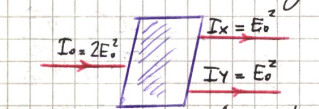
\includegraphics[width=0.4\textwidth]{images/fig_ft2_birref.jpg}

se tienen dos estados. Este sistema es similar a lo que se vio previamente. A la salida tengo
dos estados.
Lo que entrará será 
\[
	\vb E = E_0 ( \xver + \yver ) \euler^{i( kz - \omega t)}
\]
y la analogía me lleva a que polarización de luz en $\xver$ y $\yver$ equivalen a $S_z^+$ y $S_z^-$,
respectivamente.
Repetimos los experimentos, pero ahora con luz.

Matemáticamente el filtro en $\xver$ es un ente que lo que hace es proyectar la luz entrante
en $\xver$.

Los tres casos entonces corresponden a:

{\bf 1}

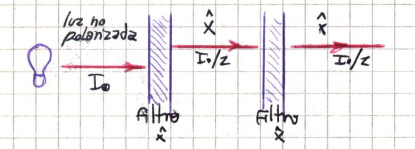
\includegraphics[width=0.5\textwidth]{images/fig_ft2_polarizacion_1.jpg}

No hay efecto neto. Opera como un filtro en $\xver$ del modo $(\vb E\cdot\xver)\xver$
y lo que sale es $E_0 \xver \euler^{i( kz - \omega t)}$

{\bf 2}

En este caso el filtro a $\pi/4$ lo que hace es proyectar en $\xver', \yver'$

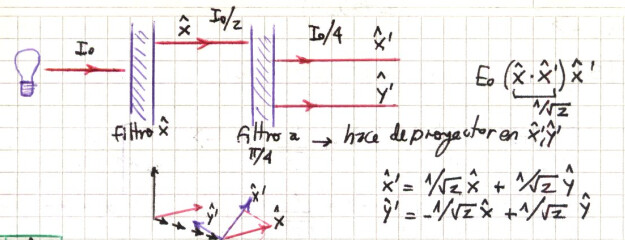
\includegraphics[width=0.5\textwidth]{images/fig_ft2_polarizacion_2.jpg}

Se tienen a la salida $E_0(\xver\cdot\xver')\xver$ donde
\[
	\xver' = \frac{1}{\sqrt{2}} \xver +  \frac{1}{\sqrt{2}} \yver \qquad \qquad 
	\yver' = -\frac{1}{\sqrt{2}} \xver +  \frac{1}{\sqrt{2}}, 
\]
de manera que $S_x^+$ equivale a $\xver'$ y $S_x^i$ equivale a $\yver'$.

{\bf 3}

Aquí se ve que filtrar dos veces es incompatible con el electromagnetismo.
A la salida se tiene $E_0(\xver'\cdot\xver)\xver$, de modo que aparece una componente
que no estaba presente.

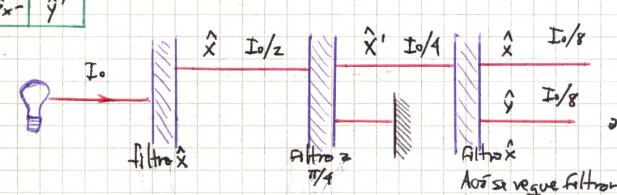
\includegraphics[width=0.5\textwidth]{images/fig_ft2_polarizacion_3.jpg}

Entonces
\[
	\vb E = E_0 \left( 
	\frac{1}{\sqrt{2}} \: \xver \cos( (kz-\omega t) ) + \frac{1}{\sqrt{2}} \: \yver \cos( (kz-\omega t) )
	\right) =
	E_0 \left( \frac{ \xver \pm i \yver }{\sqrt{2}} \right) \euler^{i(kz-\omega t)}
\]
de manera que con un cristal birrefringente que separe izquierda-derecha en luz polarizada
circular puedeo continuar la equivalencia
$S_y^+ \equiv \text{right}$ y $S_y^- \equiv \text{left}$ y tenemos seis estados pero son
solo dos los independientes.

Hacen falta vectores complejos para describir sistemas cuánticos. Ya en este sencillo caso
de analogía luz-spin vemos que la descripción completa del problema no puede hacerse en
términos de vectores con coeficientes reales.
Necesitamos un espacio complejo.

El problema del spin es sencillo porque es discreto y de dos estados.

La amplitud de probabilidad será algo como
\[
	A \sim \hat{i} \cdot \hat{j}
\]
donde j es el filtro. Luetgo la probabilidad es
\[
	P = |A|^2 = (\hat{i} \cdot \hat{j})(\hat{i} \cdot \hat{j})^*.
\]
Para operar construiremos un formalismo.

\subsection{El formalismo}

El formalismo para la mecánica cuántica incluirá
\begin{itemize}
	\item Estados
	\item Productos entre estados (propiedades matemáticas)
	\item Operadores, que llevan a observables
	\item Postulados de la mecánica cuántica
\end{itemize}

Para el caso del spin se definen
\[	
	S =\frac{1}{2} \qquad \qquad S_z^+, S_z^-
\]
y se definen los kets $\Ket{ \: }$ que tendrán toda la información. Inventados por P.A.M. Dirac.
No son otra cosa que vectores con coeficientes complejos.
La base de polarización (estados) será
\[
	\Ket{S_z;+} \qquad \qquad \Ket{S_z;-}
\]
y entonces $\Ket{S_x;+}$ es una combinación lineal de 1,2 anteriores.
Así
\[
\begin{array}{rr}
	\Ket{S_x;+} &= \displaystyle \frac{1}{\sqrt{2}} \Ket{S_z;+} + \frac{1}{\sqrt{2}} \Ket{S_z;+} \\
	& \\
	\Ket{S_x;-} &=\displaystyle  -\frac{1}{\sqrt{2}} \Ket{S_z;+} + \frac{1}{\sqrt{2}} \Ket{S_z;-} \\
	& \\
	\Ket{S_y;+} &=\displaystyle  \frac{1}{\sqrt{2}} \Ket{S_z;+} + \frac{i}{\sqrt{2}} \Ket{S_z;-} \\
	& \\
	\Ket{S_y;-} &=\displaystyle  \frac{1}{\sqrt{2}} \Ket{S_z;+} - \frac{i}{\sqrt{2}} \Ket{S_z;-}
\end{array}
\]
aunque probar esto no es ninguna boludez.


% =================================================================================================
\section{Algebra?}
% =================================================================================================

El ket contiene toda la información cuántica del estado. Da el estado físico del sistema.
Cumplen las siguientes propiedades
\begin{itemize}
	\item $\Ket{\alpha} + \Ket{\beta}$ la suma de kets es un ket
	\item $c\Ket{\alpha}= \Ket{\alpha} c$ con $c\in\mathbb{C}$
	\item $c_1\Ket{\alpha} + c_2\Ket{\beta} = \Ket{\gamma}$ con $c_1,c_2 \in \mathbb{C}$
	\item $c\Ket{\alpha},\Ket{\alpha}$ representan el mismo estado cuántico
\end{itemize}

Se define un espacio de {\it Bra} dual al de "kets" al que se va mediante ``dual conjugado''
\[
	\Ket{a}, \Ket{a'} \Leftrightarrow \Bra{a}, \Bra{a'}
\]
\[
	\Ket{a} + \Ket{b} \leftrightarrow \Bra{a} + \Bra{b} \qquad 
	c\Ket{a} \leftrightarrow c^*\Bra{a}
\]
\[
	c_a \Ket{a} + c_b \Ket{b} \leftrightarrow c_a^* \Bra{a} + c_b^*\Bra{b}
\]

Se define también un producto interno según
\[
	(\Bra{\alpha})(\Ket{\beta}) \equiv \Braket{\alpha|\beta}
\]
que no es otra cosa que un número complejo. Se puede hacer entonces una equivalencia con los vectores
estándard del álgebra del siguiente modo 
\[
	\text{ket} \sim \text{vector columna} \qquad \Ket{x} = \begin{pmatrix}
	                                                       1 \\
	                                                       0 \\
	                                                      \end{pmatrix}
\]
\[
	\text{bra} \sim \text{vector fila} \qquad \Bra{x} = ( 1 \; 0 )          
\]
y habiendo definido esta base escribimos, por ejemplo
\[
	\Ket{a} = \frac{1}{\sqrt{2}} \begin{pmatrix} 1 \\ 1  \\ \end{pmatrix}  =
	\frac{1}{\sqrt{2}} \begin{pmatrix} 1 \\ 0  \\ \end{pmatrix}  + 
	\frac{1}{\sqrt{2}} \begin{pmatrix} 0 \\ 1  \\ \end{pmatrix} =
	\frac{1}{\sqrt{2}} \Ket{x} + \frac{1}{\sqrt{2}} \Ket{y} 
\]
\[
	\Braket{a|x} = \frac{1}{\sqrt{2}}( 1 \; 1)\begin{pmatrix} 1 \\ 0  \\ \end{pmatrix} = \frac{1}{\sqrt{2}}
\]
y del mismo modo
\[
	\left( \frac{1}{\sqrt{2}} \Bra{x} + \frac{1}{\sqrt{2}} \Bra{y}  \right)
	\left( \Ket{x} \right)= \frac{1}{\sqrt{2}}.
\]
La trasposición opera como en álgebra, transmutando de ket a bra y viceversa.
\[
	\xver' = \frac{1}{\sqrt{2}}\begin{pmatrix}
	                            1 \\
	                            0 \\
	                           \end{pmatrix}
	                           \qquad \qquad 
	(\xver')^\dagger = \frac{1}{\sqrt{2}} (1 \; 0) 
\]

El producto interno tiene las siguientes propiedades:
\begin{enumerate}
	\item $\Braket{\beta|\alpha} = \Braket{\beta|\alpha}^*$ \text{luego} $ \Braket{\alpha|\alpha} \; \in \mathbb{R}$
	\item $\Braket{\alpha|\alpha} \geq 0$ \text{métrica definida positiva}
	\item $\Braket{\alpha|\beta} = \Braket{\beta|\alpha} = 0 \Leftrightarrow \Ket{\alpha} \perp \Ket{\beta}$
	\item $\Braket{\tilde{\alpha}|\tilde{\alpha}} = 1 \; \text{con} \; 
	\Ket{\tilde{\alpha}} = \frac{1}{\sqrt{\Braket{\alpha|\alpha}}}\Ket{\alpha} $ todo ket no nulo es normalizable
\end{enumerate}

La primera propiedad busca que podamos darle significado probabilístico.
El producto $\Braket{\a|\a}$ da la norma al cuadrado.

\begin{ejemplo}{\bf Veamos que el estado de spin $S_x^+$ está normalizado}

Para ello escribimos su expresión en términos de los estados $S_z$ y aplicamos dual conjugado.
Luego, 
\[
	\Braket{ S_x ; + | S_x ; + } =
	\left( \frac{1}{\sqrt{2}} \Bra{S_z;+} + \frac{1}{\sqrt{2}} \Bra{S_z;-} \right) 
	\left( \frac{1}{\sqrt{2}} \Ket{S_z;+} + \frac{1}{\sqrt{2}} \Ket{S_z;-} \right) 
\]
\[
	\Braket{S_x,+|S_x,+} =  \frac{1}{\sqrt{2}} \Braket{S_z;+|S_z;+} +
	\frac{1}{\sqrt{2}} \Braket{S_z;+|S_z;-} +
	\frac{1}{\sqrt{2}} \Braket{S_z;-|S_z;+} +
	\frac{1}{\sqrt{2}} \Braket{S_z;-|S_z;-} = 1
\]

\end{ejemplo}

Recordemos que en la formulación de mecánica cuántica que se utilizó en anteriores cursos, F4,
se tenían funciones de onda que se pueden ver como una notación relacionada con kets y bras
a través del producto interno.
\[
	\Braket{ \b | \a } = \int d^3x \: \phi^*_\b(\vbx) \: \phi_\a(\vbx) 
\]


\subsection{Operadores}

A cada observable lo representaremos por un operador. Hay operaradores que no vienen de observables.
\[
	\hat{A}\Ket{\alpha} = \Ket{\gamma} \qquad \qquad  \Bra{\alpha} \hat{A} = \Bra{\gamma}
\]
un operador sobre un ket da otro ket y sobre un bra da otro bra. Notemos que en este último caso opera 
a izquierda. Por el momento se trabajará con operadores lineales.

La transformación entre operadores se da con 
\[
	\hat{X}\Ket{a} \Leftrightarrow \Bra{a}\hat{X}^\dagger
\]
donde $\dagger$ (daga) significa el traspuesto conjugado; cambia el sentido hacia donde actúa el operador 
y conjuga. Se da que si 
\[
	\hat{X} = \hat{X}^\dagger \quad \Rightarrow \qquad \hat{X} \;\text{es hermítico}
\]
En mecánica cuántica todos los observables serán representados por operadores hermíticos.

Se dan 
\begin{itemize}
	\item $\hat{X}\hat{Y} \neq \hat{Y}\hat{X} \qquad \qquad \text{no conmutativo}$
	\item $\hat{X}(\hat{Y}\hat{Z}) = (\hat{X}\hat{Y})\hat{Z} = \hat{X}\hat{Y}\hat{Z} \qquad \qquad \text{asociativo}$
	\item $(XY)^\dagger = Y^\dagger X^\dagger$
	\item $\hat{0}\Ket{\alpha} = 0 \qquad \forall \Ket{\alpha}$ ; $\hat{0} \equiv$ operador nulo
	\item $\hat{X}( c_1 \Ket{\alpha} + c_2 \Ket{\beta} ) = c_1 \hat{X}\Ket{\alpha} + c_2 \hat{X}\Ket{\beta} $
\end{itemize}
de modo que en cuántica los observables se representan mediante operadores hermíticos.

\subsection{Sandwichs}

Coloquialmente encerrar un operador operando sobre un ket (bra) con un bra (ket).
Se obtiene un escalar
\[
	\Braket{\beta|X|\alpha} = (\Bra{\beta})(X\Ket{\alpha}) = \Braket{\beta|\gamma} =
	\Braket{\gamma|\beta}^* = (\Braket{\alpha|X|\beta})^*
\]
donde usamos que $\Ket{\gamma}$ es un ket y por dual conjugado $\Bra{\gamma} = \Bra{\alpha}\hat{X}^\dagger$ y
extraemos como conclusión 
\[
	\Braket{\beta|X|\alpha} = (\Braket{\alpha|X|\beta})^*,
\]
y de manera equivalente
\[
	\Braket{\beta|X|\alpha} = (\Bra{\beta}X^\dagger)(\Ket{\alpha}) = \Braket{\Gamma|\alpha} =
	\Braket{\alpha|\Gamma}^* = (\Braket{\alpha|X^\dagger|\beta})^*
\]
donde usamos que $\Bra{\Gamma}$ es un bra y por dual conjugado $\Ket{\Gamma} = \hat{X}\Ket{\beta}$.
El formalismo parece ser consistente. El operador opera sobre un ket/bra y multiplica al otro.

\notamargen{Las mediciones se pensarán como proyectar sobre autoestados.}

\subsection{Producto externo}

Es un nuevo tipo de producto entre vectores.
\[
	\Ket{\beta} \Bra{\alpha} \equiv (\Ket{\beta} )( \Bra{\alpha} )
\]
\[
	( \Ket{\beta} \Bra{\alpha} )\Ket{\gamma} = 
	\Ket{\beta} \Bra{\alpha} \Ket{\gamma} =
	\Braket{\alpha|\gamma} \Ket{\beta} , 
\]
de modo que es un operador pues al aplicar sobre un ket obtengo otro ket 
(notemos que $\Braket{\alpha|\gamma}$ es un escalar). Podemos pensar que 
\[
	\Lambda_\alpha \equiv \Ket{\alpha}\Bra{\alpha}
\]
es un nuevo operador, el proyector, que actúa rotando un $\Ket{\gamma}$ en 
la dirección de $\Ket{\beta}$. 
Notemos 
\[
	\Lambda_\alpha^2 = \Ket{\alpha}\Bra{\alpha}\Ket{\alpha}\Bra{\alpha} = 
	\Ket{\alpha}\Bra{\alpha} = \Lambda_\alpha
\]
puesto que $\Braket{\alpha|\alpha}=1$, de manera que aplicar dos veces un 
proyector no cambia nada.
El proyector $\Lambda_\alpha$ sobre un ket $\Ket{\beta}$ selecciona la parte de
$\Ket{\beta}$ en la dirección de $\Ket{\alpha}$. Nos dice cuanto de $\Ket{\beta}$ 
está en la dirección de $\Ket{\alpha}$.
Luego,
\[
	\sum_i^N \; \Lambda_i = \sum_i^N \; \Ket{i}\Bra{i} = \mathbb{1}
\]
la suma de todos los proyectores del espacio en el que estamos es la identidad de
ese espacio.
Decimos que $\{ \Ket{i} \}$ es un conjunto completo. 

\begin{ejemplo}{\bf Traspuesto de un producto externo}

Queremos ver que si $X = \Ket{\beta} \Bra{\alpha}$, entonces $X^\dagger = \Ket{\alpha} \Bra{\beta}$.
Hacemos operar sobre estados arbitrarios, y sabiendo que valen 
\[
	\Braket{a|X|b} = \Braket{b|X^\dagger|a}^* \qquad \qquad \Braket{a|X|b}^* = \Braket{b|X^\dagger|a}
\]
se tiene, reemplazando la definición de $X$,
\[
	 \Braket{a|(\Ket{\beta} \Bra{\alpha})|b}^* = \Braket{b|(\Ket{\beta} \Bra{\alpha})^\dagger|a}
\]
\[
	 \Braket{a|\beta}^* \Braket{\alpha|b}^* = \Braket{\beta|a} \Braket{b|\alpha} =
	 \Braket{b|\alpha}\Braket{\beta|a} = \Braket{b|(\Ket{\beta} \Bra{\alpha})|a}
\]
y comparando este último resultado con el de la línea anterior, vemos que se verifica
\[
	\Ket{\a} \Bra{\b} = (\Ket{\beta} \Bra{\alpha})^\dagger.
\]
 
\end{ejemplo}

\begin{ejemplo}{\bf Ejemplo sencillo 2D}
 
Consideramos versores en el plano, vectores columna,
\[
	\hat{X} = \begin{pmatrix} 1 \\ 0 \end{pmatrix} \qquad \qquad \hat{Y} = 
	\begin{pmatrix} 0 \\ 1 \end{pmatrix}
\]
que en sus versiones dagueadas pasan a ser vectores fila
\[
	\hat{X}^\dagger = ( 1 \; 0 ) \qquad \qquad \hat{Y}^\dagger = ( 0 \; 1  ) 
\]

Luego, los productos que podemos hacer corresponden a las operaciones matriciales de
vector por vector, resultando en número o matriz dependiendo del orden
\[
	\hat{X}^\dagger\hat{X} = (1 \; 0) \begin{pmatrix} 1 \\ 0 \end{pmatrix} = 1 \qquad 
	\hat{X}\hat{X}^\dagger = \begin{pmatrix} 1 \\ 0 \end{pmatrix} (1 \; 0) = 
	\begin{pmatrix} 1 & 0 \\ 0 & 0 \\ \end{pmatrix},
\]
donde instamos al lector a que note la diferencia de dimensión en los resultados.
En la notación de Dirac estos versores serían $\Ket{x}, \Ket{y}$ y sus correspondientes
bras. Luego,
\[
	\Braket{x|x} = \Braket{y|y} = 1, \qquad \qquad \Braket{x|y} = \Braket{y|x} = 0
\]
y las matrices serían los proyectores
\[
	P_x \equiv \Ket{x}\Bra{x}, \qquad \qquad  P_y \equiv \Ket{y}\Bra{y}.
\]

Para un estado arbitrario $\Ket{\a} = \a_x \Ket{x} + \a_y \Ket{y}$, si uso el proyector
$P_x$ se tendrá
\[
	P_x \Ket{\a} = (\Ket{x}\Bra{x})(\a_x \Ket{x} + \a_y \Ket{y})
\]
\[
	P_x \Ket{\a} = \a_x \Ket{x}\Braket{x | x} + \a_y \Ket{x}\Braket{x |y} =
	\a_x \Ket{x}.
\]
Del mismo modo se obtiene $P_y \Ket{\a} = \a_y \Ket{y}$. Si sumo ambos proyectores obtengo
la identidad
\[
	(P_x + P_y)\Ket{\a} \equiv I \Ket{\a} = \Ket{\a},
\]
y vemos que la identidad no hace nada.

\end{ejemplo}

Los kets $\Ket{\alpha}$ {\it viven} en un espacio vectorial de Hilbert con dimensión $N$, donde
$N$ lo dicta el número de posibles estados de cada sistema físico. 
Una partícula de spín $1/2$ sólo tiene dos estados: up y down.

Hay otro producto más, entre dos bras o dos kets, que se llama producto tensorial y se representa 
como 
\[
	\Ket{\alpha} \otimes \Ket{\beta} \qquad \qquad \Bra{\alpha} \otimes \Bra{\beta}
\]
que es un producto entre kets de espacios de Hilbert diferentes; el resultado no es ni un bra ni
un ket. Digamos que es una notación.
\[
	\Braket{\alpha|\beta}^* \equiv DC\{\ket{\beta}\} DC\{\Bra{\alpha}\}
\]

\section{Bases}

Dado un sistema físico representado por un espacio vectorial $\mathcal{H}$ de dimensión $N$ existirá una base (también 
de dimensión $N$) que será un conjunto de estados tal que cualquier estado de ese sistema físico puede representarse 
como combinación lineal de ese conjunto,
\[
	\{ \Ket{i}\} \; \text{base} \quad \Rightarrow \; \Ket{\alpha} = \sum_i^N c_i \Ket{i}
\]
siendo $\Ket{\alpha}$ un estado cualquiera.
Es práctico utilizar bases ortonormales,
\[
	\Braket{ i|j } = \delta_{ij} = \begin{cases}
	                                1 \quad i=j \\
	                                0 \quad i\neq j
	                               \end{cases}
\]
que es la delta de Kronecker.

Así, los kets se definen normalizados, dado un ket
\[
	\Ket{\phi} =  a \Ket{1} + b \Ket{2} + c \Ket{3}
\]
se lo normaliza con
\[
	\Ket{\psi} = \frac{1}{\Braket{\phi|\phi}}\:\Ket{\phi}
\]
lo que significa que 
\[
	\Ket{\psi} = a' \Ket{1} + b' \Ket{2} + c' \Ket{3} \qquad\qquad |a'|^2 + |b'|^2 +|c'|^2 = 1
\]
Si tenemos un ket normalizados,  $\Ket{\phi} = a \Ket{1} + b \Ket{2}$ y su bra 
$\Bra{\phi} = a^*\Bra{1} + b^* \Bra{2}$, entonces 
\begin{multline*}
 	\Braket{\phi|\phi} = (a^*\Bra{1} + b^* \Bra{2})(a \Ket{1} + b \Ket{2}) = \\
	a^*a \Braket{1|1} + b^*a\Braket{2|1} + a^*b\Braket{1|2} + b^*b\Braket{2|2} =
	|a|^2 + |b|^2 = 1
\end{multline*}
	

\subsection{Autokets y autovalores}

Si $\hat{A}\Ket{a}=c\Ket{a}$ entonces $\Ket{a}$ es autoket de $\hat{A}$ con autovalor $c$. Se suelen 
etiquetar los autoestados $\Ket{a'}, \Ket{a''}$ de modo que 
\[
	\hat{A}\Ket{a'} = a'\Ket{a'}
\]
lo cual lleva al problema espectral
\[
	\left(\hat{A} - a'\mathbb{1}\right) \Ket{a'} = 0
\]
entonces los operadores tendrán representación matricial, que cambiará según la base utilizada.
Vamos viendo que en general sólo se sabe cómo opera un operador sobre kets. La operación sobre los
bras la obtenemos usando dual conjugado.

Lo siguiente debiera ser amparado por un título como ``propiedades de operadores hermíticos''.

Deducimos entonces que
\begin{enumerate}
	\item Los autovalores de un operador hermítico son reales y los autokets correspondientes a diferentes
	autovalores son ortogonales.
	\item Los autokets de un operador son base completa del espacio de kets.
\end{enumerate}

Como ejemplo de A citemos
\[
	A\Ket{a'} = a' \Ket{a'} \quad \text{DC} \quad \Bra{a'} A^{\dagger} = \Bra{a'} A = \Bra{a'}a'^*
\]
de manera que 
\[
	\Braket{a'|A|a'} = \Bra{a'} ( A\Ket{a'} ) = a'
\]
\[
	( \Braket{a'|A|a'} )^* = ( \Bra{a'} )( A\Ket{|a'} )^* = ( \Bra{|a'}A^\dagger )( \Ket{a'} )
\]
\[
	= \Braket{a'|A|a'} = a' \qquad \Rightarrow \quad a' = a'^*.
\]
Me gusta más la otra forma, que es meter otro $a''$ así
\[
	\Braket{a''|A|a'} = a' \Braket{a''|a'} \qquad \qquad \Braket{a''|A^\dagger|a'} = a''^* \Braket{a''|a'}
\]
de manera que como
\[
	(a' - a''^*) \Braket{a''|a'} = 0,
\]
si $\Ket{a'}=\Ket{a}$ entonces $a' = a'^*$ y los autovalores son reales. En cambio si $\Ket{a'}\neq\Ket{a''}$ 
se tiene $a'\neq a''$ entonces  $\Braket{a''|a'} = 0$ y los autoestados del operador son perpendiculares.
Ya está abajo esto.

Para el caso de B se postula así. Si esto vale entonces 
\[
	\Ket{\alpha} = \sum_i^N \Ket{a_i}\Bra{a_i} \Ket{\alpha} = \sum_i^N c_i \Ket{a_i} = 
	\mathbb{1}\Ket{\alpha}
\]
pues 
\[
	\Braket{\alpha|\alpha} = \sum_{i,j}^N \Braket{ a_j|c_j^* c_i|a_i} = \sum_i^N |c_i|^2 = 1
\]
y además 
\[
	A\Ket{a'} = a'\Ket{a'} \qquad A\Ket{a''} = a''\Ket{a''} \Rightarrow 
	A(\Ket{a'} - \Ket{a''} ) = a'\Ket{a'} - a''\Ket{a''}
\]
\[
	\Braket{ a''|A|a' } = a' \Braket{ a''|a' } \qquad \Braket{ a'|A|a'' } = a'' \Braket{ a'|a'' }
\]
y ahora conjugando
\[
	\Braket{ a''|A|a' }^* = a' \Braket{ a''|a' }^* \qquad \Braket{ a''|A|a' } = a'' \Braket{ a''|a' }
\]
donde usamos que $a''^* = a''$ y restando 
\[
	(a'-a'')\Braket{a''|a'} = 0 \qquad \Rightarrow \; \Braket{a''|a'} = 0 
		\quad \text{si} \quad a'\neq a''
\]
O sea, hemos probado que los autovectores correspondientes a diferentes autovalores son
ortogonales.


\subsection{Combinación lineal de autoestados}

Podemos escribir 
\[
	\Braket{a''|a'} = \delta_{a'a''}
\]
que es la delta de Kronecker.
Postulo que forman una base completa, y que un estado $\Ket{\alpha}$ se puede escribir en 
función de la base $\Ket{a_i}$ de esta forma 
\[
	\Ket{\a} = \sum_{a'}  C_{a'} \Ket{a'}.
\]

Ahora quisiéramos ver quién es el coeficiente $C_{a'}$.
Para ello multiplicamos por un bra arbitrario
\[
	\Braket{a_j|\alpha} = \sum_{i=1}^N C_i \underbrace{\Braket{a_j|a_i}}_{\delta_{ij}} = C_j, 
\]
de modo que es
\[
	\Ket{\alpha} = \sum_{i=1}^N \Ket{a_i}\Braket{a_i|\alpha} = 
		\sum_{i=1}^N \Braket{a_i|\alpha} \: \Ket{a_i}
\]
o bien, en términos del operador $\Lambda$ [?],
\[
	\Ket{\alpha} = \left( \sum_{i=1}^N \Ket{a_i}\Bra{a_i} \right) \Ket{\alpha} 
\]
de modo que si la base es completa debe ser
\[
	\sum_{i=1}^N \Ket{a_i}\Bra{a_i} \equiv \mathbb{1}.
\]

Todos estos resultados surgen de suponer que los autoestados son una base completa.
Es análogo a la proyección de un vector en un sistema coordenado: 
$\vb V = \sum_i (\vb V\cdot \hat{e}_i ) \hat{e}_i $.

Asimismo, considerando la normalización de estados
\[
	\Braket{\a|\a} = 1 =
	\Bra{\a} \sum_{a'}\Ket{a'} \Braket{a'|\a} = \sum_{a'} \Braket{\a|a'} \Braket{a'|\a}
\]
o bien
\[
	\Braket{\a|\a} = 1 = \sum_{a'} C_{a'}^* C_{a'} = \sum_{a'} |C_{a'}|^2.
\]

% Si la base es completa entonces es $\sum \Lambda = 1$.

\subsection{Operadores y matrices}

Un operador se puede representar matricialmente como 
\[
	X = \sum_{a'}^N  \sum_{a''}^N \Ket{a''} \Bra{a''} X \Ket{a'} \Bra{a'} =  
	\sum_{a'}^N  \sum_{a''}^N ( \Braket{a''|X|a'} ) \Ket{a''} \Bra{a'}
\]
donde hemos explotado el hecho de que en el medio aparece un escalar (?), siendo 
\[
	X_{ij} = \Braket{a_i|X|a_j}
\]
un elemento de matriz. Y notemos que $\Ket{a''} \Bra{a'}$ es un ente de $N\times N$.
Si la base es de dimensión 3 se tendrá por ejemplo,
\[
	X = \begin{pmatrix}
	 x_{11} & x_{12} & x_{13} \\
	 x_{21} & x_{22} & x_{23} \\
	 x_{31} & x_{32} & x_{33} \\
	\end{pmatrix}
\]
de manera que existe una identificación entre cosas del álgebra básica y este mundo
de operadores y estados.
Si $X$ es hermítico por ejemplo, entonces su matriz es simétrica conjugada.
\[
	\Braket{a_i|X|a_j}^* = (\Bra{a_j}X^\dagger)(\Ket{a_i}) = \Braket{a_j|X|a_i}
\]
y entonces 
\[
	\Braket{a_j|X|a_i}^* = \Braket{a_i|X|a_j}
\]
de modo que 
\[
	X_{ji}^* = X_{ij} \qquad X_{ij}^{t*} = X_{ij} \qquad X_{ij}^\dagger=X_{ij}
\]
y vemos bien el significado de {\it daguear}. En este caso la matriz tiene traza real
y seis elementos independientes
\[
	X = \begin{pmatrix}
	  X_{11} & X_{12} & X_{13} \\
	  X_{12}^* & X_{22} & X_{23} \\
	  X_{13}^* & X_{23}^* & X_{33} \\
	\end{pmatrix} =
	\begin{pmatrix}
	  X_{11} & X_{12} & X_{13} \\
	  X_{21} & X_{22} & X_{23} \\
	  X_{31} & X_{32} & X_{33} \\
	\end{pmatrix} =
	\begin{pmatrix}
	  X_{11}^* & X_{21}^* & X_{31}^* \\
	  X_{12}^* & X_{22}^* & X_{32}^* \\
	  X_{13}^* & X_{12}^* & X_{33}^* \\
	\end{pmatrix}
\]

La traza será
\[
	\text{ tr }(A) = \sum_{i=1}^N \Braket{ a_i | A | a_i }.
\]


\subsection{Cambio de base}

Para cambiar de base metemos un uno ($\mathbb{1}$) escrito como suma de proyectores,
\[
	X\Ket{b_j} = \mathbb{1} \: X\Ket{b_j} = \sum_{i=1}^N \Ket{a_i}\Braket{a_i|X|b_j} = 
	\sum_{i=1}^N C_{ij} \Ket{a_i}
\]
siendo $C_{ij}$ la matriz del cambio de base.
Se puede escribir
\[
	\Ket{b_j} = \sum_{i=1}^N \Ket{a_i}\Braket{a_i|b_j} 
\]
y se ve que $\Braket{a_i|b_j}$ son los elementos de la matriz que cambia de base.

\begin{ejemplo}{\bf Ejercicio 2}

Tenemos la base $\{ \Ket{+}, \Ket{-} \}$, o sea un espacio de Hilbert de dimensión 2. Se considera
ortonormal de manera que
\[
	\Braket{+|+} = \Braket{-|-} = 1 \qquad \Braket{+|-} = 0
\]
Luego, se tiene
\[
	S_x = \frac{\hbar}{2} (\: \Ket{+}\Bra{-} + \Ket{-}\Bra{+} \:)
\]
Los elementos de matriz serán
\[
	(S_x)_{11} = \Bra{+} (S_x ) \Ket{+} =
	 \frac{\hbar}{2} \Bra{+} (\: \Ket{+}\Bra{-} + \Ket{-}\Bra{+} \:) \Ket{+} = 0,
\]
dado que ambos miembros dan $\Braket{+|-}$. Asimismo,
\[
	S_x \Ket{+} = \frac{\hbar}{2} ( \Ket{+}\Bra{-} + \Ket{-}\Bra{+} ) \Ket{+} = \frac{\hbar}{2}\Ket{-}
\]
y 
\[
	S_x \Ket{-} = \frac{\hbar}{2}\Ket{+}.
\]

Matricialmente
\[
	S_x = \frac{\hbar}{2} \: \begin{pmatrix}
	0  &  1 \\
	1  &  0
	\end{pmatrix}
\]
de manera que
\[
	S_x \Ket{+} = \frac{\hbar}{2} \: \begin{pmatrix}
	0  &  1 \\
	1  &  0
	\end{pmatrix}
	\begin{pmatrix}
	 1 \\
	 0
	\end{pmatrix}
	=
	\frac{\hbar}{2} \: 
	\begin{pmatrix}
	 0 \\
	 1
	\end{pmatrix}.
\]
 
\end{ejemplo}

\begin{ejemplo}{\bf Ejercicio 6}
 
Tenemos un espacio de kets generado por $\{ \Ket{a'} \}$ ortogonales, siendo $A$ hermítico, de
manera que los $a$ son reales.

i) Queremos probar que $\Pi_{a'} (A - a'\mathbb{1})$ es el operador nulo. Luego, supongamos que 
\[
	\Pi_{a'} (A-a'\mathbb{1}) \equiv O
\]
y entonces verificará
\[
	\Braket{a'|O|a''} = O_{a'a''} = 0.
\]
Tomemos
\[
	\Pi_{a'} (A-a'\mathbb{1}) \Ket{a''} = \Pi_{a'} A \Ket{a''} - a\mathbb{1} \Ket{a''}
	= \Pi_{a'} (\Ket{a''} + a' ) \Ket{a''}
\]
pero lo que opera sobre el ket es nulo.

Por otra parte, como $(A-a_n\mathbb{1})\Ket{a''}$ se puede escribir
\[
	(A-a_{n_2}\mathbb{1})(A-a_{n_1}\mathbb{1})\Ket{a''}( a'' - a_n )
\]
y sigue pasadno de modo que al final se obtiene
\[
	\Ket{a''} \Pi_{a'} (a'' - a').
\]

ii) Y ahora, qué significa el siguiente operador
\[
	\Pi_{a' \neq a''} \frac{ (A-a''\mathbb{1}) }{ ( a' - a'' ) }
\]
Aplicamos a un ket $\Ket{a}$,
\[
	\Pi_{a' \neq a''} \frac{ (A-a''\mathbb{1}) }{ ( a' - a'' ) } \Ket{a} = 
	\Pi_{a' \neq a''} \frac{ ( a - a'' ) }{ ( a' - a'' ) } \Ket{a}
\]
y será nulo sí y sólo si $a \neq a''$, de manera que es una construcción de la delta de Kronecker,
\[
	\Pi_{a' \neq a''} \frac{ (A-a''\mathbb{1}) }{ ( a' - a'' ) } = \delta_{aa'}\Ket{a'}
\]
Es un proyector de todos los elementos en $\Ket{a'}$ lo que siempre da cero para los de la base
salvo cuando es $a'=a$.
 
\end{ejemplo}

\begin{ejemplo}{\bf Ejercicio 8}

Consideramos $\vb S\cdot \nver$ donde $\vb S = ( S_x, S_y, S_z )$ o sea un vector de operadores y el
versor es el usual de esféricas en términos de los ángulos.
\[
	\nver = (\sin\b\cos\a, \sin\b\sin\a, \cos\b).
\]
\end{ejemplo}

\begin{ejemplo}{\bf Ejercicio 11}
 
Consideremos la matriz $M$ hermítica y la base $\{ \Ket{1}, \Ket{2}, \Ket{3} \}$ que tendrá por ello
autovalores relaes y autovectores ortogonales.
\[
	M = \begin{pmatrix}
	     0 & 1 & 0 \\
	     1 & 0 & 1 \\
	     0 & 1 & 0 
	    \end{pmatrix}
\]
Los autovalores saldrán de
\[
	\left| \frac{1}{\sqrt{2}} \begin{pmatrix}
	                         -\lambda & 1 & 0 \\  
	                         1 & -\lambda & 1 \\
	                         0 & 1 & -\lambda 
	                          \end{pmatrix}
				\right| = -\lambda(\lambda^2 -1) = 0
\]
que dará $\lambda = 0,1,-1$.
Los autovectores salen de resolver 
\[
	\begin{pmatrix}
	0 & 1/\sqrt{2} & 0 \\
	1/\sqrt{2} & 0 & 1/\sqrt{2} \\
	0 & 1/\sqrt{2} & 0 
	\end{pmatrix}
	\begin{pmatrix}
	v_1^{(1)} \\
	v_2^{(1)} \\
	v_3^{(1)}
	\end{pmatrix} = 0
\]
y haciendo $v_2^{(1)} =0$ se tiene $v_1^{(1)} =-v_3^{(1)} $ y luego
\[
	v^{(1)}  =\frac{1}{\sqrt{2}} \begin{pmatrix}
	                              1 \\
	                              0 \\
	                              -1
	                             \end{pmatrix}
\]
con $\Braket{v^{(1)}|v^{(1)}} =1$ y así siguiendo con los otros vectorcillos, resulta
\[
	A = \left[ v^{(1)} v^{(2)} v^{(3)} \right] = 
	\begin{pmatrix}
	    0 & 0 & 0 \\
	    0 & 1 & 0 \\
	    0 & 0 & -1 
	\end{pmatrix}
\]
 
\end{ejemplo}

\subsection{Representación diagonal}

Un operador tiene representación diagonal cuando está representado en la base de sus
autokets
\begin{multline*}
 	A = \sum_i^N\sum_j^N \Ket{a_i}\Braket{a_i|A|a_j}\Bra{a_j} =
		\sum_i^N\sum_j^N a_j\Ket{a_i}\Braket{a_i|a_j}\Bra{a_j} = \\
		\sum_{i,j}^N \delta_{ij} a_j \Ket{a_i}\Bra{a_j} = \sum_i^N a_i \mathbb{1}
\end{multline*}
% \[
% 	A = \sum_i^N\sum_j^N \Ket{a_i}\Braket{a_i|A|a_j}\Bra{a_j} =
% 		\sum_i^N\sum_j^N a_j\Ket{a_i}\Braket{a_i|a_j}\Bra{a_j} =
% 		\sum_{i,j}^N \delta_{ij} a_j \Ket{a_i}\Bra{a_j} = \sum_i^N a_i \mathbb{1}
% \]
\[
	A = \begin{pmatrix} 
		a_1 & 0 & ... & 0 \\
		0 & a_2 & ... & 0 \\
		0 & 0 & ... & 0 \\
		0 & 0 & ... & a_n \\
	\end{pmatrix}
\]
y $a_1,a_2,...,a_n$ son sus autovalores.
Es destacable que es conveniente utilizar como bases los autoestados de ciertos operadores.

\subsection{Representaciones canónicas}

Podemos representar una base como vectores canónicos
\[
	\Ket{a_1} = \begin{pmatrix}
			1 \\
			0 \\
			. \\
			. \\
			N
			\end{pmatrix} \qquad 
	\Ket{a_1} = \begin{pmatrix}
			0 \\
			1 \\
			. \\
			. \\
			N
			\end{pmatrix} \qquad 
	\Ket{a_n} = \begin{pmatrix}
			0 \\
			0 \\
			. \\
			. \\
			1
			\end{pmatrix}
\]
luego 
\[
	\Ket{\alpha} = \sum_i \Ket{a_i}\Braket{a_i|\alpha} =
		\Braket{a_1|\alpha} \begin{pmatrix}
			1 \\
			0 \\
			. \\
			. \\
			N
			\end{pmatrix} +
		\Braket{a_2|\alpha} \begin{pmatrix}
			0 \\
			1 \\
			. \\
			. \\
			N
			\end{pmatrix} +
			... +
		\Braket{a_n|\alpha} \begin{pmatrix}
			0 \\
			0 \\
			. \\
			. \\
			1
			\end{pmatrix} =
\]
\[
	\begin{pmatrix}
		\Braket{a_1|\alpha} \\
		\Braket{a_2|\alpha} \\
			... \\
			... \\
		\Braket{a_n|\alpha}
	\end{pmatrix}
\]
y por DC se tiene 
\[
	\Bra{\alpha} = ( \; \Braket{\alpha|a_1} \quad \Braket{\alpha|a_2} 
	\quad ... \quad \Braket{\alpha|a_n} \; )
\]
y 
\[
	\Braket{\alpha|\alpha} = 1 = \overbrace{( \phantom{1} \qquad \phantom{1} )}^{1\times 
N}\overbrace{\begin{pmatrix} \phantom{1} \\ 	\phantom{1}  \end{pmatrix} }^{N\times 1} = \Box
\]
que es un escalar.
El producto entre otros dos estados arbitrarios
\[
	\Braket{\beta|\alpha} = \Braket{\beta|a_i} \Braket{a_i|\alpha} = 
	\sum_i^N \Bra{\beta} \underbrace{\Ket{a_i} \Bra{a_i}}^{\Lambda_{a_i}} \Ket{\alpha} = \Box 
\]
otra vez un escalar.

Para un operador $X$ se tiene la siguiente representación
\[
	X = \sum_i^N \sum_j^N \Ket{a_i} \Braket{a_i|X|a_j} \Bra{a_j} =
		\sum_i^N \sum_j^N  \Braket{a_i|X|a_j} \Ket{a_i} \Bra{a_j}
\]
y esto último es una matriz. Aquí el $\hat{X}$ es una matriz y 
$\Braket{a_i|\hat{X}|a_j} \equiv X_{ij}$ son sus elementillos (escalares).
En conclusión,
\[
	X = \sum_i^N \sum_j^N X_{ij} \: \Ket{a_i} \Bra{a_j},
\]
donde 
\[
	\Ket{a_i} \Bra{a_j} = \begin{pmatrix}
	 0 \\
	 ... \\
	 1 \\
	 ... \\
	 0
	\end{pmatrix}
	(\: 0 .... 1 .... 0 \:).
\]

Para un operador que actúa sobre un estado, dando otro estado, se tiene
\[
	\Braket{a_i|\gamma} = \Braket{a_i|X|\alpha} = \sum_{a_j} \Braket{a_i|X|a_j}\Braket{a_j|\alpha}
\]
que es el producto de una matriz por un vector
\[
	\begin{pmatrix}
	 \Braket{a_1|\gamma} \\
	 ... \\
	 ... \\
	\end{pmatrix} = 
	\begin{pmatrix}
	 X_{11} & X_{12} & ...\\
	 X_{21} & X_{22} & ... \\
	 ... \\
	\end{pmatrix}
	\begin{pmatrix}
	 \Braket{a_1|\alpha} \\
	 ... \\
	 ... \\	 
	\end{pmatrix}
\]

Para el producto externo será
\[
	\Ket{\b}\Bra{\a} = \sum_{a',a''} \Ket{a''} \Braket{a''|\b} \Braket{\a|a'} \Bra{a'}
\]
y este producto de brakets es la versión matricial del operador
\[
	\begin{pmatrix}	
	\Braket{a_1|\b} \Braket{a_1|\a}^* & \Braket{a_1|\b} \Braket{a_2|\a}^* & ... \\
	\Braket{a_2|\b} \Braket{a_1|\a}^* & \Braket{a_2|\b} \Braket{a_2|\a}^* & ... \\
	... & ... & 
	\end{pmatrix}
\]

En la base en la cual un operador es diagonalizable resulta sencilla su matriz:
\[
	A = \sum_{a',a''}  \Ket{a''} \Braket{a''|A|a'} \Bra{a'} = 
	\sum_{a'}  a' \Ket{a'} \Bra{a'} = \sum_{a'}  a' \Lambda_{a'},
\]
en términos del proyector.

Los elementos usados en el formalismo (bras, kets, etc.) pueden pensarse como vectores (fila
o columna) y matrices.

% ~~~~~~~~~~~~~~~~~~~~~~~~~~~~~~~~~~~~~~~~~~~~~~~~~~~~~~~~~~~~~~~~~~~~~~~~~~~~~~~~~~~~~~~~~
\section{Sistemas de spín 1/2}

Hay dos estados posibles de spin,
\[
	\Ket{S_z ; +} = \Ket{S_z = \hbar/2} \equiv \Ket{+} 
	\qquad \qquad 
	\Ket{S_z ; -} = \Ket{S_z = -\hbar/2} \equiv \Ket{-}
\]
de manera que la dimensión del espacio vectorial es 2. 
Entonces, la identidad será 
\[
	\mathbb{1} = \Ket{+}\Bra{+} \; + \;  \Ket{-}\Bra{-}
\]

\notamargen{Acá hay que diseñar unos $+,-$ que habiten dentro de los brakets pues estos se ven feo.}

Luego, en la representación de $S_z$ se tiene
\[
	S_z \ket{+} = \frac{\hbar}{2} \Ket{+} \qquad \qquad 
	S_z \ket{-} = \frac{\hbar}{2} \Ket{-},
\]
que viene de que el operador es
\[
	S_z = \frac{\hbar}{2} \left( \: \Ket{+}\Bra{+} \: - \: \Ket{-}\Bra{-} \: \right).
\]
Luego,
\[
	S_+ \equiv \hbar  \Ket{+}\Bra{+}  \qquad 
	S_- \equiv \hbar  \Ket{-}\Bra{-} 
\]
donde $S_- = S_+^\dagger$ son operadores de subida y de bajada.
que actuarán subiendo/bajando el spin o dando el ket nulo.
Así,
\[
	S_+ \Ket{-} = \hbar \Ket{+} 
	\qquad \qquad  
	S_- \Ket{+} = \hbar \Ket{-} 
	\qquad \qquad 
	S_+ \Ket{+} = S_- \Ket{-} = 0
\]

En la representación vectorial serán
\[
	\Ket{+} \equiv \begin{pmatrix} 1 \\ 0 \end{pmatrix}
	\qquad \qquad 
	\Ket{-} \equiv \begin{pmatrix} 0 \\ 1 \end{pmatrix}
\]
de manera que los proyectores
\[
	\Lambda_+ = \Ket{+}\Bra{+} =  \begin{pmatrix} 1 & 0 \\ 0 & 0 \end{pmatrix}
\]
\[
	\Lambda_- = \Ket{-}\Bra{-} =  \begin{pmatrix} 0 & 0 \\ 0 & 1 \end{pmatrix}
\]
luego
\[
	\Lambda_+ + \Lambda_- = \begin{pmatrix} 1 & 0 \\ 0 & 1 \end{pmatrix}
\]

Los operadores $\pm$ serán
\[
	S_+ = \hbar \begin{pmatrix} 1 \\ 0 \end{pmatrix} ( 0 \; 1 ) 
		= \hbar \begin{pmatrix}  0 & 1 \\ 0 & 0 \end{pmatrix}
	\qquad \qquad 
	S_- = \hbar \begin{pmatrix} 0 \\ 1 \end{pmatrix} ( 1 \; 0 ) 
		= \hbar \begin{pmatrix} 0 & 0 \\ 1 & 0 \end{pmatrix}
\]
de modo que
\[
	S_+ \Ket{-} = \hbar \begin{pmatrix}  0 & 1 \\ 0 & 0 \end{pmatrix}
	\begin{pmatrix} 0 \\ 1 \end{pmatrix} = 
	\hbar \begin{pmatrix} 1 \\ 0 \end{pmatrix} = \hbar \Ket{+}.
\]
Finalmente,
\[
	\Ket{S_x ; \pm} = \frac{1}{\sqrt{2}} \left( \: \Ket{S_x ; +} \pm \Ket{S_x ; -} \: \right).
\]

\subsection{Cambio de base}

Dados dos conjuntos $\{ \Ket{a'} \}, \{ \Ket{b'} \} $ base ortonormales y completos 
existe un $\widehat{U}$ unitario tal que :
\[
	U^+U=UU^+=\mathbb{1} \qquad \text{ con }\qquad \Ket{b_i}=U\Ket{a_i}
\]

Este operador de cambio de base será 
\[
	U = \sum_\ell \Ket{b_\ell}\Bra{a_\ell}
\]
y actuando sobre un elemento de la base $a$,
\[
	U\Ket{a_i} = \sum_\ell \Ket{b_\ell}\Braket{a_\ell|a_i} = \Ket{b_i}
\]

Este operador $U$ cumple la función de pasar entre bases
\[
	\underbrace{\Ket{a_\ell}}_{\text{vieja base}} 
	\qquad 	\longrightarrow \qquad 
	\underbrace{\Ket{b_\ell}}_{\text{nueva base}}
\]
o bien
\[
	\Ket{\text{nueva base}} = U \Ket{\text{vieja base}}.
\]
Notemos que
\[
	U U^\dagger = \sum_{k,\ell} \Ket{a^k} \Braket{b^k | b^\ell} \Bra{a^\ell} =
	\sum_{k} \Ket{a^k}\Bra{a^k} = \mathbb{1}
\]
donde del segundo al tercer miembro se pasa por la ortogonalidad de la base $b$.

Veamos cómo transforma un ket genérico, usando que
\[
	\Braket{ a^k | U | a^\ell } = \Bra{ a^k } \sum_j \Ket{ b^j } \Braket{ a^j | a^\ell } = 
	\Braket{ a^k | b^\ell }.
\]
Un ket arbitrario se escribirá como una combinación lineal de la base $a$, es decir,
\[
	\Ket{\a} = \sum_{\a'} \Ket{a'}\Braket{a'|\a}
\]
de modo que 
\[
	\Braket{b_k|\alpha} = \sum_\ell \Braket{b_k|a_\ell}  \Braket{a_\ell|\alpha}  =
	\sum_\ell \Braket{a_k|U^+|a_\ell}  \Braket{a_\ell|\alpha} = \Braket{a_k|U^+|\alpha} 
\]
e identificamos
\[
	 \Braket{b^k|a^\ell} = \Braket{a_k|U^+|a_\ell} 
\]
que nos convierte de 
\[
	\Ket{\text{nueva base}} = U^\dagger \Ket{\text{vieja base}}.
\]
Esta es la relación consistente con la anterior en términos de $U$ [?].

Por otra parte, considerando otro operador $X$
\[
	\Braket{b_i | X | b_j} = \sum_{\ell,m} \Braket{b_i|a_\ell}\Braket{a_\ell|X|a_m}\Braket{a_m|b_j },
\]
o bien,
\[
	\Braket{b_i | X | b_j} = \sum_{\ell,m}\Braket{a_i|U^+|a_\ell}\Braket{a_\ell|X|a_m}\Braket{a_m|U|a_j}
\]
lo cual implica que
\[
	X_{\Ket{b}} = U^+ X_{\Ket{a}} U,
\]
que es una transformación de similaridad.

\notamargen{En matrices se puede poner como:
\[
	X'_{kl} = U_{km}^\dagger X_{mn} U_{nl}.
\]}

\subsection{Mediciones y probabilidades}

En mecánica cuántica medir es filtrar; de todos los autoestados posibles se selecciona uno de ellos. 
La medición perturba al sistema. Se miden variables dinámicas asociadas a observables.
Como los autoestados de un observable $\hat{A}$ son una base completa $\{\Ket{a_i}\}$ entonces un sistema se hallará en 
una combinación lineal de autoestados de $\hat{A}$, o al menos eso puede pensarse.


\begin{tabular}{|c|c|c|}
\hline
antes de medir & Medición de $\hat{A}$ & luego de medir \\
\hline 
sistema en CL
de autestados de $\hat{A}$ &  & Salta a un autoestado de $\hat{A}$ \\
\hline 
sistema en 
autoestado de $\hat{A}$  & & Continúa en autoestado de $\hat{A}$ \\
\hline
\end{tabular}

Puede verse pictóricamente la medición así:
\[
	\Ket{\alpha} \qquad \longrightarrow \qquad \Ket{a'}
\]
el proceso de medición hace saltar $\Ket{\a}$ hacia $\Ket{a'}$, siendo el resultado de 
la medida el autovalor $a'$.
Antes de medir no puedo saber a qué estado saltará y tampoco en qué estado se hallaba. 
Si antes de medir se hallaba en un autoestado, continúa manteniéndose allí
\[
	\Ket{a'} \qquad \longrightarrow \qquad \Ket{a'}
\]

Lo que se puede determinar es la probabilidad de que se halle en cierto autoestado
$a'$ de acuerdo con 
\[
	\mathrm{Prob}_{\Ket{a'}} \equiv |\Braket{a'|\alpha}|^2.
\]

Si $P=1$ se halla en $\Ket{a'}$ antes de saltar, si $P=0$ no se halla en $\Ket{a'}$ 
antes de saltar. Este valor de $\mathrm{Prob}$ es mayor igual a cero y se verifica
\[
	\sum_{a'} \mathrm{Prob}_{a'} = 1
\]
si la probabilidad está correctamente normalizada.

\notamargen{La base que diagonaliza a un operador es la de sus autoestados.}

Notamos que se puede escribir
\[
	P = \Braket{a'|\a}\Braket{\a|a'} = \Braket{\a |\Lambda_{a'}| \a}
\]

\subsection{Valor de expectación}

\[
	\Braket{\widehat{A}} \equiv \Braket{\alpha|A|\alpha}
\]c
el valor de expectación siempre se refiere a un estado en particular.
\[
	\Braket{A} = \sum_{a',a''} \Braket{\alpha|a'}	\Braket{a'|A|a''} \Braket{a''|\alpha}
\]
\[
	\Braket{A} = \sum_{a',a''}  \Braket{\alpha|a'} a''\delta_{a'a''} \Braket{a''|\alpha} =
			\sum_{a''} a''|\Braket{\alpha|a''}|^2
\]
\[
	\Braket{A} = \sum_{a',a''} = a'' \text{Prob}_{\Ket{a''}}
\]
Esto último tiene el sentido de una especie de promedio ponderado.
Hasta repetir el cansancio el experimento el resultado tenderá a este valor de expectación.


\subsection{Conmutadores}

Dados dos operadores $A, B$, se definen, el conmutador
\[
	[ A, B] \equiv AB - BA,
\]
y el anticonmutador
\[
	\{ A, B \} \equiv AB + BA,
\]
y se dice que dos observables conmutan si $[A,B]=0$. Se dice que son compatibles si $[A,B]=0$
y anticompatibles si se da la contrario, $[A,B]\neq 0$.

TEOREMA:

Sean dos observables compatibles y no degenerados, entonces los autoestados $\{ \Ket{a'}\}$ de $A$ lo son también de 
$B$. Es decir que A y B tienen base de autoestados en común.

demostración:
\[
	\Braket{a'|AB-BA|a''} = 0 
\]
\[
	a' \Braket{a'|B|a''} - \Braket{a'|B|a''} a''= (a'-a'') \Braket{a'|B|a''}= 0 
\]
entonces 
\[
	\Braket{a'|B|a''} = 0
\]
y $B$ es diagonal en $\{ \Ket{a'}\}$.
Luego, se ve que escribiendo B en términos de esta base y aplicando sobre un estado de la misma
\[
	B \Ket{a''} = \sum \Ket{a'} \Braket{a'|B|a'} \Braket{a'|a''} = \Braket{a''|B|a''} \Ket{a''}
\]
por lo tanto la base de $A$ diagonaliza a $B$, pero los autoestados tienen todos sus autovalores diferentes.

Los autoestados son iguales pero no los autovalores; con lo cual se utilizará la notación $\Ket{a',b'}$ donde 
\[
	A \Ket{a',b'} = a' \Ket{a',b'} \qquad \qquad B \Ket{a',b'} = b' \Ket{a',b'}
\]

Si dos operadores no conmutan entonces no hay base común para ambos.
Para ver que se debe cumplir esto supongamos que sí hay base común.
Entonces, se tendrán
\[
	AB \Ket{a',b'} = b' A \Ket{a',b'} =  b' a' \Ket{a',b'}
\]
\[
	BA \Ket{a',b'} = a' B \Ket{a',b'} =  a' b' \Ket{a',b'}
\]
y estos dos renglones son iguales puesto que números escalares sí conmutan.
Luego,
\[
	AB \Ket{} = BA \Ket{}
\]
y entonces como esto significa que conmutan y partimos de la presunción en contrario,
con lo cual este absurdo surge de asumir base en común; no la tienen.
Por ende no los puedo medir con precisión. La medida del segundo afecta a la medición del primero.

\subsection{Degeneración}

Puede darse que haya varios $g$ autoestados correspondientes a un mismo autovalor $a'$; 
entonces se dice que hay degeneración de orden $g$ para el autoestado $\Ket{a'}$
\[
	A\Ket{a'}= a'\Ket{a'} \quad ; i=1,2,...,g
\]
y $A$ tendrá una matriz de $m\times n$ bloques. 
En este caso no se puede decir que la base de $A$ diagonalice a $B$.
\notamargen{Mejorar la matriz que está un asco}
\[
	A = \begin{pmatrix}
	     a'\mathbb{1} & 0 & & \\
	     0 & a''\mathbb{1} & & \\
	     & & a'''& \\
	     & & & a^IV \\
	     ...
	    \end{pmatrix}
\]
Los $\ket{a'_i}$ no dan información sobre los bloques correspondientes en la matriz de $B$.
Necesito un conjunto de operadores que haga romper la degeneración para expresar unívocamente 
el estado del sistema. Se llama CCOC. Necesito que conmuten entre sí para que las mediciones tengan sentido.
Un Conjunto Completo de Observables que Conmutan.

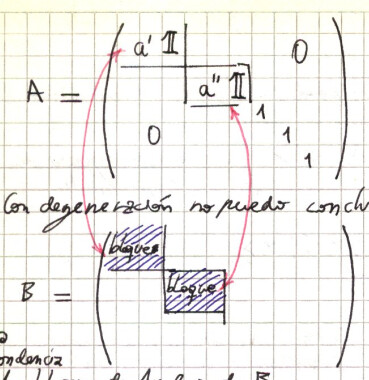
\includegraphics[width=0.5\textwidth]{images/fig_ft2_matriz_degenerada1.jpg}

Si no conmutan entonces son incompatibles; la medición de uno hace saltar al sistema a un autoestado del otro y como no 
son comunes pierde sentido el concepto de medir. No tiene sentido la medición de algo si por el hecho de medir 
cambiamos lo que queremos medir.
Al ser incompatibles sus mediciones de afectan mutuamente.

Los autovalores de algunos operadores podrán tener degeneración pero una combinación de los autovalores del CCOC, 
$\Ket{a'b'c'...}$, determina el estado de forma única.

Dado un set CCOC, $\{A,B,C,D\}$, se etiquetarán $\Ket{K'} \equiv \Ket{a'b'c'd'}$ los autoestados,
que es una variable colectiva.
Se cumplirán
\[
	\Braket{K | K'} = \delta_{KK'} = \delta_{aa'} \delta_{bb'} ...
\]
\[
	\sum_{K'} \Ket{K'}\Bra{K'} = \mathbb{1}
\]
Las únicas cosas que tiene sentido medir en MC son las variables asociadas a operadores en un CCOC.

Sean $A,B$ compatibles sin degeneración, y consideremos la siguiente notación pictórica donde
arriba digo qué mido y abajo qué obtengo. Entonces
\[
	\Ket{\alpha} \overbrace{\underbrace{\longrightarrow}_{a'}}^{\text{Mido A}} \Ket{a'b'}
	\overbrace{\underbrace{\longrightarrow}_{b'}}^{\text{Mido B}} \Ket{a'b'} 
	\overbrace{\underbrace{\longrightarrow}_{a'}}^{\text{Mido A}} \Ket{a'b'}
\]
Veo que midiendo alternadamente uno y otro no salgo del autoestado $\Ket{K'}$. 

En cambio si $A,B$ son compatibles pero con degeneración en el autoestado $a'$ [?] se tiene
\[
	\Ket{\alpha} \overbrace{\underbrace{\longrightarrow}_{a'}}^{\text{Mido A}} 
		\sum_{i=1}^g C_{a'}^{(i)}\Ket{a'b'(i)} \overbrace{\underbrace{\longrightarrow}_{b'(j)}}^{\text{Mido B}} 
		C_{a'}^{(j)}\Ket{a'b'(j)} \overbrace{\underbrace{\longrightarrow}_{a'(j)}}^{\text{Mido A}} 
		C_{a'}^{(j)} \Ket{a'b'(j)}
\]

Al medir A y obtener $a'$ no tengo determinado el estado del sistema (medir A no me da información). 
Me hallaré en una CL de autoestados correspondientes al autovalor degenerado $a'$. Al medir luego B 
selecciono uno de los $\Ket{a'b'}$ degenerados, el correspondiente a $b'(j)$ pues B no está degenerado. 
Puedo volver a medir A pues el autoestado en que ha caído el fsistema permanece incólume.

\subsubsection{Operadores y observables}

Entonces siendo $A$ un operador se dice que es un observable si el operador es hermítico, con lo cual
sus autovalores serán reales, y si el conjunto de sus autoestados es una base.
Usando la notación $\Ket{a,i}$ para indicar un autoestado y su degeneración, se tiene una 
descomposición espectral
\[
	A = \sum_{a,i} a \KB{a,i}{a,i}
\]
que se puede asociar a una matriz como
\[
	\begin{pmatrix}
	1 & ... &  & & \\
	... & 2 & & & \\
	... & & 2 & & \\
	... & & & 3 &  \\
	... & & & & 
	\end{pmatrix}
\]
Luego,
\[
	A = 1 \KB{1,1}{1,1} + 2 \left( \KB{2,1}{2,1} + \KB{2,2}{2,2}\right) + ...
\]

El espacio de los operadores es $N$, finito. En el caso de $N \to \infty$ hay que sumar algunas
restricciones (me pregunto si tiene que ver con alguna regularización para evitar infinitos).
Se dice que A es normal si verifica $[A,A^\dagger] = 0$.

\subsection{Postulados de la mecánica cuántica}

\begin{enumerate}
	\item El estado de un sistema lo definimos con un ket $\Ket{\alpha} \in \mathcal{H}$ y
		con $\Braket{\alpha|\alpha}=1$
	\item Asociamos a propiedades físicas (observables) operadores hermíticos $\widehat{A}$ 
		que operan sobre los kets. Los autokets $\Ket{a}$ verifican :
	\[
		\widehat{A}\Ket{a} = a \Ket{a}, 
	\]
	y $\{ \Ket{a} \}$ es base del espacio de kets. El operador se puede expresar como
	\[
		A = \sum_{a,i} a \KB{a,i}{a,i}
	\]
	\item Al medir una cantidad física representada por el observable $\widehat{A}$ obtenemos
	siempre un autovalor $a'$.
	Luego de medir, el estado del sistema es $\Ket{a}$.
	Suponiendo un estado $\Ket{\Psi}$, sobre el cual se mide $A$ (obteniéndose $a$), se tendrá que
	inmediatamente después el estado de $\Ket{\Psi'}$ según
	\[
		\Ket{\Psi} \overbrace{\underbrace{\longrightarrow}_{a'}}^{\text{Mido A}} \Ket{\Psi'} =
		P_a \Ket{\Psi} = \Ket{a}\Braket{a|\Psi} =(\Braket{a|\Psi})\Ket{a}
	\]
	Llevé al sistema a un autoestado de $\widehat{A}$. 
	\notamargen{No confundir la notación para proyector con la de probabilidad.}
	Ahora quizás deba ahora normalizar, es decir
	\[
		\Ket{\Psi'}_\text{norm} = \frac{\Braket{a|\Psi}}{\sqrt{\Braket{\Psi'|\Psi'}}} \: \Ket{a}
	\]
	donde $\Braket{\Psi'|\Psi'}=\Braket{\Psi|P_a P_a|\Psi} = \Braket{\Psi|P_a|\Psi}$, siendo la
	última igualdad porque $P_a$ es un proyector y su cuadrado es él mismo.
	El esquema de arriba representa la frase ``proyectar sobre la base de autoestados''.
	
	Dos posibilidades al medir. Si la probabilidad la nomenclamos como $P(a)$ que es la probabilidad
	de medir el estado $a$, entonces
	\begin{itemize}
	 \item Sin degeneración:
	 \[
		P(a) = |\Braket{a|\psi}|^2
	 \]
	 \item Con degeneración:
	 \[
		P(a) = \sum_{i} |\Braket{a,i|\psi}|^2
	 \]
	\end{itemize}
	\item Las transformaciones espaciales se generan por $\vb{p}$
	\[	
		[x_i,p_j] = i\hbar\delta_{ij}
	\]
	\item La evolución temporal la realiza $H$ (el hamiltoniano).
\end{enumerate}

\notamargen{Extrañamente el punto 4 estaba vacío. Raro.}

\subsection{Operador de dispersión}

Se define la dispersión del operador $A$ de acuerdo con
\[
	\Delta \widehat{A} \equiv \widehat{A} - \Braket{A}\mathbb{1}
\]
la dispersión será nula cuando el sistema se halle en un autoestado del operador $\widehat{A}$. 
Será no nula en caso contrario, cuando no se halle en un autoestado.
Luego la dispersión cualitativamente nos dice ``qué tan lejos'' del autoestado nos hallamos.
\begin{multline*}
	\Braket{(\Delta A)^2} = \Braket{(\widehat{A} - \Braket{A}\mathbb{1})^2} =
	\Braket{ A^2 - 2A\Braket{A} + \Braket{A}^2 } = \\
	\Braket{A^2} - 2A\Braket{A}^2 + \Braket{A}^2 = \Braket{A^2} - \Braket{A}^2
\end{multline*}
y la relación de dispersión generalizada
\[
	\Braket{(\Delta A)^2} \Braket{(\Delta B)^2} \geq \frac{1}{4}|\Braket{[ A,B ]}|^2
\]
se probará [?].

\begin{ejemplo}{\bf Ejercicio 9 guía 1}

Espacio de spines de dimensión 2. Base $\{ \Ket{+}, \Ket{-} \}$.
Consideramos un versor angular con ángulos $\a, \b$ según se ilustra aquí abajo.

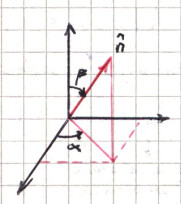
\includegraphics[width=0.225\textwidth]{images/fig_ft2_ejercicio91.jpg}

Del ejercicio 8 se sabe que
\[
	\Ket{\vb S\cdot\nver; +} = \cos(\b/2) \Ket{+} + \sin(\b/2) \euler^{i\a} \Ket{-}
\]
Luego, como $ \vb S\cdot\nver \Ket{\vb S\cdot\nver; \pm} = \pm \hbar/2 \Ket{\vb S\cdot\nver; \pm } $ 
se tiene
\[
	P\Frac{\hbar}{2} = |\Braket{S_x;+| \vb S\cdot\nver ; +}|^2
\]
donde usando que 
\[
	\Ket{S_x;+} = \frac{1}{\sqrt{2}} \left( \Ket{+} + \Ket{-} \right)
\]
nos conduce a
\[
	P\Frac{\hbar}{2} = \frac{1}{2} | \cos(\b/2) + \sin(\b/2) \euler^{i\a} |^2
\] 
y usando $\a=0, \b=\gamma $ resultan en
\[
	P\Frac{\hbar}{2} = \frac{1}{2} \left( 1 + \sin\gamma \right).
\]

En la parte b) se pide hallar $\Delta S_x^2 = \vm{S_x^2}- \vm{S_x}^2 $. Para ello
usamos los hallazgos del ejercicio 2.
\[
	S_x = \frac{\hbar}{2} \left[ \KB{+}{-} + \KB{-}{+} \right]
\] 
y luego
\[
	S_x^2 = \frac{\hbar^2}{4}\left[ \KB{+}{+} + \KB{-}{-} \right] = 
	\frac{\hbar^2}{4}\mathbb{1}
\]

Entonces,
\[
	\vm{S_x^2} = [ \cos(\gamma/2) \Bra{+} + \sin(\gamma/2) \Bra{-} ] S_x^2
	[ \cos(\gamma/2) \Ket{+} + \sin(\gamma/2) \Ket{-} ]
\]
Se puede ver que
\[
	\vm{S_x} = \frac{\hbar}{2} \sin\gamma,
\]
de manera que lo buscado es
\[
	(\Delta S_x)^2 = \frac{\hbar^2}{4} \cos^2\gamma.
\]
 
 
\end{ejemplo}


\begin{ejemplo}{\bf Ejercicio 10}

Se tiene la situación ilustrada en las figuras bajo estas líneas

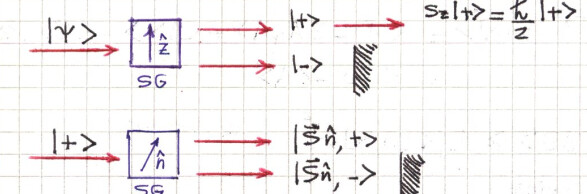
\includegraphics[width=0.45\textwidth]{images/fig_ft2_ejercicio10A.jpg}

Por otra parte, la probabilidad será
\[
	P\Frac{\hbar}{2}_{\nver} = |\Braket{S_n,+|+}|^2 = \cos^2\Frac{\b}{2}
\]

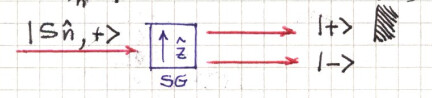
\includegraphics[width=0.45\textwidth]{images/fig_ft2_ejercicio10B.jpg}

Consiguientemente,
\[
	P\Frac{-\hbar}{2}_{\nver} = |\Braket{-|\vb S\cdot\nver,+}|^2 = \sin^2\Frac{\b}{2}
\]
y la intensidad final
\[
	I_f = I_0 \: \cos^2\Frac{\b}{2} \: \sin^2\Frac{\b}{2}.
\]
 
\end{ejemplo}



\begin{ejemplo}{\bf Ejercicio 12}
 
Consideramos una base $\{ \Ket{a',b'} \}$ ortonormal de autoestados de $\vb A\cdot \vb B$.
La idea es que $ [A,B] = C$ si $C\Ket{\Psi} = 0 \forall \Ket{\Psi}$.
Entonces lo aplicamos a algo
\[
	(AB - BA)\Ket{\Psi} = c\Ket{\Psi}
\]
\[
	A\Ket{a'b'} = a' \Ket{a'b'}  \qquad \qquad B\Ket{a'b'} = b' \Ket{a'b'}
\]
 
\end{ejemplo}

\subsection{Espectro continuo}

Queremos pasar al continuo este formalismo. Pensamos en una única variable $x$, tal que
\[
	x \Ket{x'} = x' \Ket{x'}
\]
y los kets de la base son los canónicos. En un rango $[a,b]$ descomponemos una función
$f_N(x)$ en esta base
\[
	\Ket{f_N} = f_N(x_1) \Ket{x^{(1)}} + f_N(x_2) \Ket{x^{(2)}} + ...
	+ f_N(x_N) \Ket{x^{(N)}},
\]
o bien
\[
	\Ket{f_N} = \sum_{i=1}^N \: f_N(x_i) \Ket{x^{(i)}}
\]
y queremos pasar al continuo utilizando $N \to \infty$ y $\Delta x \to 0$ con la constraint
de que $N\Delta x \to cte.$

Hay observables con espectro de autovalores continuo.
Nos podemos construir la siguiente tabla para comparar ambos escenarios.

\begin{tabular}{|c|c|}
\hline 
Espectro discreto & Espectro continuo \\
\hline
  & \\
  $A\Ket{a'}=a'\ket{a'}$ & $Y\Ket{y'}=y'\ket{y'}$ \\
  & \\
  $\mathbb{1} = \sum_{a' }^N \Ket{a'}\Bra{a'} $ & $\mathbb{1} = 
  \int_{-\infty}^ {\infty} \Ket{y'}\Bra{y'} dy' $ \\
  & \\
  $\Braket{a'|a''} = \delta_{a' a''}$ & $\Braket{y'|y''} = \delta(y'-y'')$ \\
  & \\
  $ \sum_{a' }^N \Braket{a'|a''}\Bra{a''} = \Bra{a'}$ & 
  $ \int_{-\infty}^\infty dy'' \Braket{y'|y''}\Bra{y''} = \Bra{y'}$ \\
  & \\
  $ \sum_{a' }^N \Ket{a'} \Braket{a'|\alpha} = 
  \Ket{\alpha}$ & $ \int_{-\infty}^\infty dy' \Ket{y'}\Braket{y'|\alpha} = \Ket{\alpha}$ \\
  & \\
  $ \sum_{a' }^N |\Braket{a'|\alpha}|^2 = 1$ & 
  $ \int_{-\infty}^\infty dy'|\Braket{y'|\alpha}|^2 = 1$ \\  & \\
  $ \Braket{\beta | \alpha}  = \sum_{a' }^N \Braket{\beta|a'}\Braket{a'\alpha}$ & 
  $ \Braket{\beta | \alpha}  = \int_{-\infty}^\infty dy' \Braket{\beta|y'}\Braket{y'\alpha}$ \\
  & \\
\hline  
\end{tabular} 

Debemos notar aquí que la delta correspondiente al caso discreto es la de Kronecker,
mientras que la del caso continuo es la de Dirac.

\subsection{Midiendo y otras representaciones. Función de onda}

El operador que da la posición es $\hat{x}$ de acuerdo con $\hat{x}\Ket{x'} = x'\Ket{x'}$.
La representación de un cierto estado es
\[
	\Ket{\alpha} = \int_{\infty}^\infty dx' \Ket{x'}\Braket{x'|\alpha},
\]
i.e. combinación lineal de todos los estados $x'$ entre $-\infty$ y $\infty$. No obstante puede
ser que al medir, la física del instrumento o de la medida nos restringe a una zona
$x \pm \Delta$, de modo que
\[
	\Ket{\alpha} = \int_{x-\Delta}^{x+\Delta} \: dx' \Ket{x'}\Braket{x'|\alpha},
\]
donde 
\notamargen{Acá ya vamos viendo que hay bases de posición, spin, momento, etc.}
\[
	\Braket{x'|\alpha}dx'
\]
es la densidad de probabilidad de hallar a la partícula entre $(x-\Delta,x+\Delta)$ y 
\[
	|\Braket{x'|\alpha}|^2
\]
es la amplitud de probabilidad. 
En el formalismo de Schrödinger la densidad de probabilidad es la función de onda
\[
	\Psi_\alpha(x) = \Braket{x|\alpha}
\]
siendo este el vínculo entre la representación de Dirac y la función de onda,
que nos permite ir de una a otra representación.
La probabilidad de hallar al sistema en $\a$ será
\[
	| \Psi_\alpha(x) |^2 = \Psi_\alpha(x) \Psi^*_\alpha(x) = | \Braket{x|\alpha} |^2.
\]
Asimismo,
\[
	\Braket{p|x} = \frac{1}{\sqrt{2 \pi \hbar}} \euler^{i p x / \hbar}.
\]

\[
	\Braket{\beta|\alpha} = \int dx' \Braket{\beta|x'}\Braket{x'|\alpha} = 
		\int dx' \Psi_\beta^*(x) \Psi_\alpha(x)
\]
Para un elemento de matriz se tiene
\[
	\Braket{\beta|A|\alpha} = 
	\int \int dx' dx''\Braket{\beta|x''}\Braket{x''|A|x'}\Braket{x'|\alpha}
\]
\[
	\Braket{\beta|A|\alpha} = 
	\int \int dx' dx'' \Psi_\beta^*(x'') \Braket{x''|A|x'} \Psi_\alpha(x')
\]
y si $A=f(\hat{x})$ entonces $f(\hat{x}) \Ket{x'} = f(x') \Ket{x'}$ y
\[
	\Braket{\beta|A|\alpha} = 
	\int \int dx' dx'' \Psi_\beta^*(x'') f(x')\delta(x''-x') \Psi_\alpha(x')
\]
y entonces 
\[
	\Braket{\beta|A|\alpha} = \int dx' \Psi_\beta^*(x') f(x') \Psi_\alpha(x').
\]

En forma análoga tenemos la representación de momento;
\[
	\hat{p}\Ket{p'} = p'\Ket{p'} \qquad \Braket{p'|p''} = \delta(p'-p'') \qquad 
	\Ket{\alpha} = \int dp' \Ket{p'}\Braket{p'|\alpha}
\]
\[
	\Phi_\alpha(p') = \Braket{p'|\alpha}.
\]

En el anterior curso de física donde se hizo algo de mecánica cuántica (F4) todo
se llevó a cabo en la representación de posición.
El formalismo de Dirac permite movernos cómodamente entre cualesquiera de estas
representaciones.

Para la generalización a 3 dimensiones se usan operadores vectoriales, que no son otra
cosa que tres operadores escalares.
\[
	\vb x \Ket{\vb{x}'} = \vb{x'} \Ket{\vb{x'}},
\]
así $y \Ket{\vb{x}'} = y' \Ket{\vb{x}'} = y' \Ket{x',y',z'}$ con
\[
	\mathbb{1} = \int_{-\infty}^{\infty} \: d^3x \KB{ \vb{x'} }{ \vb{x'} }
\]
y la delta de Dirac es
\[
	\Braket{\vb{x''}|\vb{x'}} = \delta^3(\vb{x''} - \vb{x'}) =
	\delta( x'' - x' )\delta( y'' - y' )\delta( z'' - z' )
\]


\subsection{Operador de traslación}

Este operador realiza una traslación infinitesimal.
Se le pedirá
\[
	\Tau_{(dx')} \Ket{x'} = \Ket{x'+dx'}
\]
siendo este requerimiento intuitivamente adecuado para una traslación. 
Nótese que $dx'$ no es un operador, es el parámetro de la traslación.

Sobre un ket genérico será
\[
	\Tau_{(dx')} \Ket{\a} = \int d^3x' \: \Ket{x'+dx'} \Braket{x|\a}.
\]

Cumplirá las propiedades
\begin{itemize}
 \item Unitariedad:
 \[
	\Tau^\dagger\Tau = \Tau \Tau^\dagger = \mathbb{1}
 \]
 para que no varíe la probabilidad ante un cambio de coordenadas.
 \item Aditividad:
 \[
	\Tau_{(dx')}\Tau_{(dx'')} = \Tau_{(dx'+dx'')}
 \]
 porque vale en mecánica clásica.
 \item Existencia de inverso:
 \[
	\Tau_{(dx')}^{-1} = \Tau_{(-dx'')}
 \]
 \item Existencia de la identidad, el que no hace nada. Límite a $\mathbb{1}$
 \[
	\Tau_{(dx')} \to \mathbb{1} \quad \text{si} \quad dx' \to 0
 \]
\end{itemize}

Se propone un\footnote{Es una especie de expansión de Taylor.} 
\[
	\Tau_{(dx')} = \mathbb{1} - i \vb{K}\cdot d\vb{x}'
\]
con $\vb{K}$ un operador vectorial hermítico (notemos que $\tau$ no es hermítico). 
Para ver quién es éste operador se considera
\[
	\Tau_{(dx')}^\dagger = \mathbb{1} + i \vb{K}\cdot d\vb{x}',
\]
y luego, a orden lineal, es $ \Tau_{(dx')} \Tau_{(dx')}^\dagger \approx 1$ y
\[
	\Tau_{(dx')} \Tau_{(dx)} = 1 - i \vb{K}\cdot ( d\vb{x}' + d\vb{x} )
	= \Tau_{(dx' + dx)}
\]

Comparando con mecánica clásica, y viendo que allí \vb{p} origina las traslaciones, 
entonces identificamos $\vb K$ con $\vb p$. Se postuló que 
\[
	\vb K = \frac{1}{\hbar} \vb p,
\]
y se ha visto a posteriori que esto funcionar.
\notamargen{Hay que ver el carácter vectorial de estas cosas.
$dx$ es vectorial en realidad, pero no un operador.}

Entonces pedimos que \vb{p} cuántico origine las traslaciones
\[
	\vb{K} = \frac{\vb{p}}{\hbar} \qquad \Tau_{(dx')} = 
	\mathbb{1} - \frac{i}{\hbar} \vb{P}\cdot d\vb{x}'
\]
y así
\[
	\Tau_{(dx')}\Ket{p'} =
	\left( \mathbb{1} - \frac{i}{\hbar} \vb{P}\cdot d\vb{x}' \right)\Ket{p'} =
	\left( 1 - \frac{i}{\hbar} p' dx \right)\Ket{p'}
\]
el autovalor no es real, pues $\Tau$ no es hermítico.

Partiendo del conmutador 
\[
	x \Tau_{(dx')} - \Tau_{(dx')} x = dx \Tau_{(dx')}
\]
\notamargen{En la carpeta el conmutador da sin la $\Tau$, así que acá parece
estar mal.}
entonces 
\[
	[x, \Tau_{(dx')}] = dx\Tau 
\]
y con $dx\sim 0$ a orden uno (esto significa que tiramos los términos cuadráticos en $dx$).
Usando la anterior
\[
	[x, 1 - i \vb K \cdot d\vb{x'} ] = -i [ x_i, K_j dx_j' ] = 
	-i [ x_i, K_j ] dx_j' =  dx_j'
\]
de lo cual se deduce que
\[
	\dtot{x_i'}{x_j'} = - i [ x_i , K_j ] = \delta_{ij}
\]
lo que conduce a 
\[
	[ x_i, p_j ] = i \hbar \:\delta_{ij},
\]
% \[
% 	[ x, p_x ] = i \hbar
% \]
que es la incompatibilidad de posición y momento.
% \[
% 	[ x_i, p_j ] = i \hbar \delta_{ij}.
% \]

Pero las traslaciones en diferentes direcciones conmutan
\[
	[ \Tau_{(d\vb{x}')}, \Tau_{(d\vb{x}'')} ] = 0  \qquad [ p_i, p_j ] = 0
\]
	
\[
	\Tau_{(d\vb{x}')} \Ket{\vb{p'}} = 
	\left( 1 - \frac{i}{\hbar} \vb{P'}\cdot d\vb{x} \right) \Ket{\vb{p'}}
\]
donde recordamos que como el operador no es hermítico el autovalor no es 
necesariamente real.

Sumando infinitas traslaciones infinitesimales tenemos una traslación finita,
\[
	\Tau_{(\Delta x')} = \lim_{N\to \infty}
	\left( 1 - \frac{i}{\hbar}p\frac{\Delta x'}{N}\right)^N =
	\euler^{-i/\hbar \: p\Delta x'}
\]
que en tres dimensiones será 
\[
	\Tau_{(\Delta x')} = \euler^{-i/\hbar\: \vb{p}\cdot\Delta \vb{x}'},
\]
donde se hace $ dx' \equiv \Delta x'/N $ para el paso al continuo.

\begin{ejemplo}{\bf Ejercicio 15}

Las partes a), b), c) están hechas en el libro de Sakurai.
La dispersión resulta $\vm{(\Delta A)^2} = \vm{A^2} -\vm{A}^2$ lo que es fácil de
ver haciendo explícitamente la operación para un estado $\psi$.
Se considera
\[
	\Delta A = A - \vm{A}_\psi.
\]

Si A, B son observables, entonces
\[
	\vm{\Delta A^2}_\psi \vm{\Delta B^2}_\psi \geq \frac{1}{4} |\vm{[A,B]}|^2_\psi.
\]
 
\end{ejemplo}

\begin{ejemplo}{\bf Ejercicio 16}

Tenemos $ \vm{\Delta S_x^2 } = \vm{\Delta S_x^2 } - \vm{\Delta S_x }^2 $  con $ \Ket{\psi} = \Ket{+} $
y escribimos $S_x$ en la base de autoestados
\[
	S_x = \frac{\hbar}{2} \left( \KB{+}{-} + \KB{-}{+} \right),
\]
\[
	S_x^2 = \frac{\hbar^2}{4} \left( \KB{+}{+} + \KB{-}{-} \right) = \frac{\hbar^2}{4} \mathbb{1}
\]
y como es un Stern-Gerlach en $\xver$ y le mandamos partículas en $\zver$,
\[
	\vm{S_x} = \Bra{+} S_x \Ket{+} = 0 \qquad \qquad \vm{S_x^2} = \frac{\hbar^2}{4}
\]
y de la misma manera
\[
	\vm{S_y} = 0 \qquad \qquad \vm{S_y^2} = \frac{\hbar^2}{4}
\]

Si queremos ahora probar la relación de incerteza generalizada, será
\[
	\frac{1}{4}|\vm{(S_x,S_y)}|^2 = \frac{\hbar^2}{4}|\vm{ S_z }|^2 = \frac{\hbar^4}{16},
\]
y luego
\[
	\vm{ (\Delta S_x)^2 }_{\Ket{+}} \vm{ (\Delta S_y)^2 }_{\Ket{+}} = 
	\frac{1}{4} |\vm{[S_x,S_y]}|^2_{\Ket{+}},
\]
vemos que se verifica la igualdad en la relación de incerteza.
 
\end{ejemplo}

\begin{ejemplo}{\bf Ejercicio 15 parte d)}

Se tiene
\[
	\Braket{x'|\a} = (2\pi d^2)^{-1/4} \euler^{i \vm{p}x'/\hbar - (x'-\vm{x})^2/(4d^2)}
\]
y se pide
\[
	\vm{(\Delta x)^2} \vm{(\Delta p)^2} = \frac{\hbar}{2}
\]

Son los valores medios
\[
	\vm{x} = \Braket{\a|x|\a} = 
	\int_{-\infty}^\infty \: \Braket{\a|x|x'}\Braket{x'|\a} dx' =
	\int_{-\infty}^\infty \: x' \Braket{\a|x'}\Braket{x'|\a} dx'
\]
y
\begin{multline*}
	\vm{p} = \Braket{\a|p|\a} = 
	\int_{-\infty}^\infty \: p' \Braket{\a|p'}\Braket{p'|\a} dp' = \\
	\int_{-\infty}^\infty \int_{-\infty}^\infty \int_{-\infty}^\infty \: 
	p' \Braket{\a|x'}\Braket{x'|p'}\Braket{p'|x''}\Braket{x''|\a} dp' dx' dx''
\end{multline*}
donde hemos introducido identidades, continuas, en estados de posición.
Reacomodando las integraciones,
\[
	\vm{p} =
	\int \int dx' dx'' \: \frac{\psi^*(x') \psi(x'')}{2\pi\hbar} 
	\int dp' \: p' \euler^{i p /\hbar (x' - x'')} 
\] 
y haciendo aparecer explícitamente una derivada espacial (ayudados por la exponencial)
\[
	\vm{p} =
	\int \int dx' dx'' \: \frac{\psi^*(x') \psi(x'')}{2\pi\hbar} 
	\frac{\hbar}{i} \dpar{}{x'} \int dp' \: \euler^{i p /\hbar (x' - x'')}. 
\]
Luego, como la expresión de la delta de Dirac es
\[
	\delta(x'-x'') = \frac{1}{2\pi\hbar} \int dp' \euler^{i p'/\hbar (x'-x'')}
\]
se tiene
\[
	\vm{p} = \int \int dx' dx'' \frac{\hbar}{i} \psi^*(x') \psi(x'') \delta(x'-x'') =
	\int dx' \: \psi^*(x') \left( -i \hbar \dpar{}{x'} \right) \psi(x').
\]

\end{ejemplo}

\subsection{\vb{p} en la representación \vb{x}}

\[
	\Tau_{(\Delta x)} \Ket{\alpha} = \int dt' \Tau\Ket{x'}\Braket{x'|\alpha} = 
		\int dt' \Ket{x'+ \Delta x}\Braket{x'|\alpha} = \int dt' \Ket{x'}\Braket{x'-\Delta x|\alpha}
\]
pero
\[
	\dpar{}{x'} \Braket{x'|\alpha} \approx \frac{ -\Braket{x'-\Delta x|\alpha} + \Braket{x'|\alpha} }{\Delta x}
\]
y entonces
\[
	-\dpar{}{x'} \Braket{x'|\alpha} \Delta x + \Braket{x'|\alpha}  = \Braket{x'-\Delta x|\alpha}
\]

\[
	\Tau\Ket{\alpha} = \int dx' \Ket{x'}\left( \Braket{x'|\alpha} -\dpar{}{x'} \Braket{x'|\alpha} \Delta x \right) =
	\int dx' \Ket{x'} \Braket{x'|\alpha} - \int dx' \Ket{x'}  \dpar{}{x'} \Braket{x'|\alpha} \Delta x 
\]
\[
	\left( 1 - \frac{i}{\hbar}p\Delta x \right) \Ket{\alpha} = 
		\Ket{\alpha} - \int dx' \Ket{x'}  \dpar{}{x'} \Braket{x'|\alpha} \Delta x
\]
\[
	\frac{i}{\hbar}p\Delta x \Ket{\alpha} = \int dx' \Ket{x'}  \dpar{}{x'} \Braket{x'|\alpha} \Delta x
\]
y así
\[
	p\Ket{\alpha} = -i\hbar \int dx' \Ket{x'}  \dpar{}{x'} \Braket{x'|\alpha}
\]
de modo que usándo este resultado se tienen
\[
	\Braket{x''|p|\alpha} = -i\hbar \int dx' \Braket{x''|x'}  \dpar{}{x'} \Braket{x'|\alpha}
\]
\[
	\Braket{x''|p|\alpha} = -i\hbar \dpar{}{x'} \Braket{x''|\alpha}
\]
\[
	\Braket{\beta|p|\alpha} = \int dx' \Braket{\beta|x'} (-i\hbar) \dpar{}{x'} \Braket{x'|\alpha}
\]
\[
	\Braket{\beta|p|\alpha} = \int dx' \Psi_\beta^*(x') (-i\hbar) \dpar{}{x'} \Psi_\alpha(x')
\]
de lo que se deduce 
\[
	\hat{p} \equiv - i \hbar \dpar{}{x},
\]
que es el resultado más importante de la sección.

\subsection{Cambio entre representaciones \vb{x} y \vb{p} }

\[
	\Braket{x'|\hat{p}|p'} =  -i\hbar \int dx'  \Braket{x'|x'} \dpar{}{x'} \Braket{x'|p'} =
	-i\hbar \dpar{}{x'} \Braket{x'|p'}
\]
y entonces,
\[
	p' \Braket{x'|p'} = -i\hbar \dpar{}{x'} \Braket{x'|p'},
\]
que es una ecuación diferencial para $\Braket{x'|p'}$. Luego
\[
	\int  \frac{1}{\Braket{x'|p'}} \partial \Braket{x'|p'} = 
	\int \frac{ip'}{\hbar} \partial x'
\]
\[
	\log \Braket{x'|p'} = \frac{ip'x'}{\hbar} + Cte.
\]
\[
	\int dp' \Braket{x'|p'} \Braket{p'|x''} = \Braket{x'|x''} = \delta(x-x')
\]
\[
	\int dp' \euler^{ip'/\hbar(x'-x'')} |N|^2 = \delta(x-x')
\]
\[
	|N| = \frac{1}{\sqrt{2\pi\hbar}}.
\]
\[
	\Braket{x'|p'} = \frac{1}{\sqrt{2\pi\hbar}} \euler^{i p'x'/\hbar}
\]
Con este escalar podemos cambiar entre representaciones.
Usando esto podemos ver que $\Psi_\alpha(x')$ y $\Phi_\alpha(p')$ son transformadas 
de Fourier la una de la otra.
\[
	 \int_{-\infty}^\infty dp \euler^{iap(x-x')} = \frac{2\pi}{a}\delta(x-x')
\]

\begin{ejemplo}{\bf Ejercicio 18}

$S_y$ es un operador complejo. Luego
\[
	S_y = \frac{\hbar}{2} \begin{pmatrix}
	                       0 & -i \\
	                       i & 0
	                      \end{pmatrix}
\]
Luego, dependiendo de la base que se utilice resultará
\[
	S_y|_\text{base} = \frac{\hbar}{2} \begin{pmatrix}
	                       1 & 0 \\
	                       0 & -1
	                      \end{pmatrix}
\]
 
\end{ejemplo}

\begin{ejemplo}{\bf Ejercicio 20}

Se define $f(A)$ de modo que si $f(x) = \sum_j c_j x^j$ entonces se toma
\[
	f(A) \equiv \sum_{j=0}^\infty \: c_j A^j,
\]
luego, si nos hallamos en autoestado de $A$ estaremos entonces en autoestados de $f(A)$.

Si es $A\Ket{a'} = a' \Ket{a'}$, será
\[
	A^j\Ket{a'} = A^{j-1}A\Ket{a'} = A^{j-1}a'\Ket{a'} = {a'}^j\Ket{a'}.
\]
El elemento de matriz
\[
	\Braket{b''|f(A)|b'} =  \sum_{a'} \Braket{b''|f(A)|a'} \Braket{a'|b'} =
	\sum_{a'} f(a')\Braket{b''|a} \Braket{a'|b'}
\]
y los dos últimos brakets son los datos conocidos.
La parte b) es igual pero para el caso continuo.
 
\end{ejemplo}

\subsection{Corchetes de Poisson versus conmutadores}

Hay una equivalencia entre corchetes de Poisson y conmutadores, a saber:
\[
	[A, B]_{\text{classic}} \longrightarrow \frac{1}{i\hbar}[A,B]
\]
o
\[
	[A, B]_{\text{classic}} = \sum_i \left( \dpar{A}{q_i} \dpar{B}{p_i} - \dpar{A}{p_i} \dpar{B}{q_i} \right)
\]

% \bibliographystyle{CBFT-apa-good}	% (uses file "apa-good.bst")
% \bibliography{CBFT.Referencias} % La base de datos bibliográfica

\end{document}

	
		\documentclass[10pt,oneside]{CBFT_book}
	% Algunos paquetes
	\usepackage{amssymb}
	\usepackage{amsmath}
	\usepackage{graphicx}
% 	\usepackage{libertine}
% 	\usepackage[bold-style=TeX]{unicode-math}
	\usepackage{lipsum}

	\usepackage{natbib}
	\setcitestyle{square}

	\usepackage{polyglossia}
	\setdefaultlanguage{spanish}
	



	\usepackage{CBFT.estilo} % Cargo la hoja de estilo

	% Tipografías
	% \setromanfont[Mapping=tex-text]{Linux Libertine O}
	% \setsansfont[Mapping=tex-text]{DejaVu Sans}
	% \setmonofont[Mapping=tex-text]{DejaVu Sans Mono}

	%===================================================================
	%	DOCUMENTO PROPIAMENTE DICHO
	%===================================================================

\begin{document}

% =================================================================================================
\chapter{Dinámica cuántica}
% =================================================================================================

Queremos ver la evolución temporal de los kets. Para ello utilizaremos cierta convención.
Un ket dependerá del tiempo lo cual se indicará con 
\[
	\Ket{\alpha,t_0,t},
\]
notación que refiere al estado $\alpha$ que partió en $t_0$ al tiempo $t$. 
Luego $\Ket{\alpha,t=t_0} \equiv \Ket{\a}$.
Pictóricamente
\[
	\Ket{\alpha,t_0} \underbrace{\longrightarrow}_{\text{evoluciona}} \Ket{\alpha,t_0,t}
\]

Emplearemos para ello un operador de evolución temporal $U_{(t,t_0)}$ al cual le pediremos
que realice la evolución según
\[
	\Ket{\alpha,t_0,t} = U \Ket{\alpha,t_0}
\]
Entonces, un elemento de matriz $\Braket{b|U_{(t,t_0)}|a}$ implica la probabilidad (amplitud)
de que se tenga componente de $b$ en el tiempo $t$ del sistema que estamos considerando.
El operador de evolución tendrá las propiedades

\begin{itemize}
 \item Unitariedad
 \[
	\Braket{ \alpha,t_0,t| \alpha,t_0,t} = 1 \qquad \forall t
 \]
 \[
	\Braket{ \alpha,t_0| U^\dagger U| \alpha,t_0} = 1 \quad \Rightarrow \quad 
	U^\dagger U = U U^\dagger = \mathbb{1}
 \]
 para conservación de la probabilidad. Tiene que ser unitario.
 \item Linealidad
 \[
	U(t_2,t_0) = U(t_2,t_1) U(t_1,t_0) \qquad t_2>t_1>t_0
 \]
 \item Límite a $\mathbb{1}$ (identidad)
 \[
	U_{(t,t_0)} \to \mathbb{1} \quad \text{si} \quad t\to t_0
 \]
 o bien 
 \[
	U_{(t_0+dt,t_0)} \to \mathbb{1} \quad \text{si} \quad dt\to 0
 \]
\end{itemize}

Una forma más general de escribir un $U$ unitario es $U = \euler^{i \eta A}$. De aquí se ve más fácil
que como $ \euler^{i \eta A} \euler^{-i \eta A^\dagger} = 1 $ una transformación unitaria infinitesimal es
$ U = 1 + i \eta A $ y $ - dt/\hbar = \eta $.

Se propone entonces (infinitesimalmente) un 
\[
	U_{(t+dt,t)} = \mathbb{1} - i \: \Omega \: dt 
\]
con $\Omega$ hermítico. Comparando con clásica vemos que $H$ origina la evolución temporal, entonces
identificamos $\Omega$ con $H$, del modo $\Omega = H/\hbar$ así que 
\[
	U_{(t+dt,t)} = \mathbb{1} - \frac{i}{\hbar} H dt .
\]
\notamargen{El hamiltoniano $H$ es un operador ahora.}

De esta forma 
\[
	U_{(t+dt,t_0)} =  U_{(t+dt,t)} U_{(t,t_0)}  = 
	\left( \mathbb{1} - \frac{i}{\hbar} H dt \right) U_{(t,t_0)}
\]
\[
	\dpar{U}{t} = \lim_{dt\to 0} \frac{ U_{(t+dt,t_0)} - U_{(t,t_0)} }{dt} = 
	- \frac{i}{\hbar}H U_{(t,t_0)}
\]
y entonces 
\[
	i\hbar\dpar{U}{t} = HU
\]
que es la ecuación para $U_{(t,t_0)}$.
No podemos utilizar los métodos que usamos anteriormente porque en
$U = N \euler^{i \int dt' \:H(t)/\hbar }$ [depende del tiempo?].
Supongmos que es $ H \sim \vb S \cdot \vb r (\theta)$, se tiene en
$t=0$ es $\vb r(t) = \zver$ y en $t = 5 \text{ seg. } $ es $\vb r(t) = \yver$.
Tenemos
\[
	i\hbar\dpar{}{t} U_{(t,t_0)} \Ket{\alpha,t_0} = H U_{(t,t_0)} \Ket{\alpha,t_0},
\]
que nos conduce a la ecuación de Schrödinger para kets
\[
	i\hbar\dpar{}{t} \Ket{\alpha,t_0,t} = H \Ket{\alpha,t_0,t}
\]
donde el inconveniente es que $H=H(t)$.

El concepto se ilustra en la figura siguiente
\begin{figure}[htb]
	\begin{center}
	\includegraphics[width=0.3\textwidth]{images/teo2_5.pdf}	 
	\end{center}
	\caption{}
\end{figure} 

% % =================================================================================================
% \section{Dinámica cuántica}
% % =================================================================================================

\section{Casos sencillos de solución de $U(t,t_o)$}

\begin{itemize}
 \item Supongamos $ H \neq H(t)$, entonces
 \[
	U( t, t_0) = \euler^{-i/\hbar H (t-t_0)} 
 \]
 \item Sea $ H = H(t)$, entonces
 \[
	U( t, t_0) = \euler^{-i/\hbar \int_{t_0}^t H(t')dt'} 
 \]
 y la integral puede hacerse una vez conocida la expresión de $H(t)$.
 \item Sea $ H = H(t)$ con $[H(t_1),H(t_2)] \neq 0$ entonces
 \begin{multline*}
	U( t, t_0) =  1 + \sum_{n=1}^{\infty} \left( \frac{-i}{\hbar}\right)^n 
		\int_{t_0}^t dt_1 \int_{t_0}^{t_1} dt_2 \int_{t_0}^{t_2} dt_3 ... \times \\
			\int_{t_0}^{t_{n-1}} dt_n H(t_1) H(t_2) ... H(t_n)    
 \end{multline*}
%  \[
% 	U( t, t_0) =  1 + \sum_{n=1}^{\infty} \left( \frac{-i}{\hbar}\right)^n 
% 		\int_{t_0}^t dt_1 \int_{t_0}^{t_1} dt_2 \int_{t_0}^{t_2} dt_3 ... \int_{t_0}^{t_{n-1}} dt_n 
% 			H(t_1) H(t_2) ... H(t_n)  
%  \]
y esta es la serie de Dyson (del físico Freeman Dyson().)
Esta es la solución formal general para el caso 3. 
\end{itemize}

El problema que suscita es debido a que si $H$ a diferentes tiempos no conmuta
no podemos poner la exponencial en serie de potencias. 
En realidad $\exp({\square})$ tiene sentido sólo si la serie 
\[
	\sum_{n=0}^{\infty}  \frac{1}{n!}\square^n
\]
tiene sentido; es decir, si no surgen ambigüedades al tomar la potencia $n$-ésima
del operador $\square$.
\notamargen{El operador $\square$ no se deja poner sombreros, 
quiere andar con la cabeza descubierta}

Para el caso 1 (pensamos una especie de serie de Taylor, que es un modo general
de encarar este tipo de problemas de cosas no bien definidas) es simplemente 
\[
	\euler{-i\frac{H}{\hbar}(t-t_0)} = 1 - i\frac{H}{\hbar}(t - t_0) + 
	\frac{(-i)^2}{2}\left( \frac{H \Delta t }{\hbar} \right)^2 + ... +
	\frac{(-i)^n}{n!} \Frac{H\Delta t}{\hbar}^n,
\]
y por otra parte
\[
	i \hbar \dpar{}{t}U(t,t_0) = H - i \frac{H^2}{\hbar^2} \Delta t + ...
\]
y término a término coinciden; entonces probamos que la solución vale.

Para el caso 2, donde los hamiltonianos a diferentes tiempos conmutan entre
sí, es decir $ [ H(t_1), H(t_2) ] = 0 $ la solución es
\[
	U(t,t_0) = \euler^{ i/\hbar \int_{t_0}^t \: H(t') \: dt' }
\]

Esto no es una boludez. Al desarrollar Taylor la exponencial surge un problema

Si no conmutan los operadores no sé cómo armar el cuadrado.
\[
	A^2 = A(t)A(t'') \; \text{ o bien } \: A^2 = A(t'')A(t)
\]
\[
	\left( \int H(t') dt' \right)\left( \int H(t'') dt'' \right) \neq 
	\left( \int H(t'') dt'' \int H(t') dt' \right)
\]
puesto que al operar es 
\[
	\int dt' dt'' H(t')H(t'') \neq \int dt' dt'' H(t'') H(t') 
\]
pues $[H(t'),H(t'')]\neq 0$.
En el caso 2 $(\int_{t_0}^t H(t')dt' )^n$ no tiene problemas puesto que está 
provista la conmutatividad.

\subsection{Soluciones útiles}

La solucion que sirve es
\[
	\Ket{\a,t_0,t} = U(t,t_0)\Ket{\a}
\]
La idea es escribir el $\Ket{\a}$ del sistema y hallar un operador que conmute
con el hamiltoniano y en cuya base escribo $\Ket{\a}$,
\[
	\Ket{\a} = \sum C_{a'} \Ket{a'}
	\qquad \qquad 
	H \Ket{\a} = \sum E_{a'} C_{a'} \Ket{a'}
\]
y trabajaremos con una solución útil ahora.

Primeramente conseguimos un $\hat{A}$ tal que $[ A, H ]=0$ y entonces (estoy 
considerando $ H \neq H(t)$ )
\[
	\Ket{\alpha} = \sum_{a'} \Ket{a'}\Braket{\alpha'|\alpha},
\]
luego 
\[
	U(t,t_0)\Ket{\alpha} = \sum_{a'} \euler^{-i\frac{\hat{H}}{\hbar}(t-t_0)}
	\: \Ket{a'}\Braket{\alpha'|\alpha}
\]
con $\hat{H}$ y $\hat{A}$ conmutan se tiene
\[
	\hat{H}\Ket{a'}=E_{a'}\Ket{a'} \qquad \hat{A}\Ket{a'}= a'\Ket{a'}
\]

Entonces operamos con el $H$ para 
\[
	U(t,t_0) = \sum_{a'} \euler^{-i\frac{E_{a'}}{\hbar}(t-t_0)}\Ket{a'}\Bra{a'}
\]
y así (quiero saber cómo trabaja en el tiempo $\Ket{\a}$), le aplico el operador
evolución
\[
	U(t,t_0)\Ket{\alpha} = \sum_{a'} 
	\euler^{-i\frac{E_{a'}}{\hbar}(t-t_0)}\Ket{a'}\Braket{a'|\alpha}
\]
\[
	\Ket{\alpha,t_0,t} = \sum_{a'} \Braket{a'|\alpha}
	\euler^{-i\frac{E_{a'}}{\hbar}(t-t_0)} \: \Ket{a'} =
	\sum_{a''} \sum_{a'} c_{a'} \euler^{-i\frac{E_{a'}}{\hbar}(t-t_0)} \: 
	\Ket{a''}\Braket{a''|a'}
\]
o bien
\[
	\Ket{\alpha,t_0,t} = \sum_{a'} 
	c_{a'} \euler^{-i\frac{E_{a'}}{\hbar}(t-t_0)} \: \Ket{a'},
\]
de manera que comparando con 
\[
	\Ket{\alpha,t_0} = \sum_{a'} \Braket{a'|\alpha} \Ket{a'}
\]
El coeficiente es el mismo pero le hemos sumado una fase 
$\exp(-iE_{a'}(t-t_0)/\hbar)$ que no es global.

\subsection{Evolución de valores de expectación}

Recordemos primeramente que los autoestados no evolucionan. Luego 
\[
	\Ket{\alpha} = \Ket{a'} 
	\qquad \to \qquad 
	\Ket{\alpha,t} = \Ket{a',t} =  
	\euler^{-i\frac{E_{a'}}{\hbar}(t-t_0)} \Ket{a'}
\]

La fase es global y no tiene sentido físico (no cambia el valor de expectación, por ejemplo)
Es considerar una autoestado [?]. La podemos descartar (setear igual a uno)
\[
	\Braket{a',t|B|a',t} = 
	\braket{a'|\euler^{i\frac{E_{a'}}{\hbar}(t-t_0)}B 
	\euler^{-i\frac{E_{a'}}{\hbar}(t-t_0)}|a'} = \braket{a'|B|a'}
\]

El valor de expectación de un operador respecto a un autoestado no varía.
Se simplifican las fases y en el valor de expectación no me entero de ellas.
Para un estado que no es necesariamente autoestado
\[
	\braket{\alpha,t|B|\alpha,t} =
	\braket{a''|\sum_{a''} \braket{a''|\alpha}^*\euler^{i\frac{E_{a'}}{\hbar}(t-t_0)} B 
	\sum_{a'} \braket{a'|\alpha} \euler^{-i\frac{E_{a'}}{\hbar}(t-t_0)}|a'}
\]
\[
	\braket{\alpha,t|B|\alpha,t} = \sum_{a',a''} C_{a''}^* C_{a'} 
	\euler^{i\frac{E_{a''}-E_{a'}}{\hbar}(t-t_0)} \braket{a''|  B |a'}
\]
donde $(E_{a''}-E_{a'})/\hbar$ es la llamada frecuencia de Bohr y vemos que la fase
global depende de los índices de las sumatorias; entonces habrá términos de interferencia.
\[
	C_{a''}^* = \braket{\alpha,t_0|a''} \qquad C_{a'} = \braket{a'| \alpha,t_0}  
\]

El valor de expectación de un operador respecto a un estado general tiene una fase no global 
que produce términos de interferencia.

Sólo en el caso en que $B$ conmute con $H$ ($B$ diagonal) se dará que la fase no interviene,
porque pierdo una sumatoria merced a una delta de Kronecker que aparece.

\subsection{Relaciones de conmutación}

Algunas propieadades de los conmutadores
\[
	[ A + B, C] = [A, C] + [B,C] 
\]
\[
	[A, B] = - [B,A]
\]
\[
	[A, B\cdot C] = B[A,C] +  [A,B]C
\]
Identidad de Jacobi
\[
	[ A, [B,C] ] +  [ B, [C,A] ] + [ C, [A,B] ] = 0.
\]

\notamargen{Acá no es baca + caballo puesto que no conmutan.}
\[
	i\hbar[ A, B]_{\text{classic}} = [A, B]
\]
donde $[ , ]_{\text{classic}}$ es el corchete de Poisson.
Las relaciones de conmutación fundamentales son 
\[
	[x_i, x_j] = 0 \qquad [p_i, p_j]=0 \qquad [x_i,p_j] =i\hbar\delta_{ij}
\]
a las que podemos sumar
\[
	[x,f(p)] = i\hbar\dpar{f}{p} \qquad [p,G(x)] = i\hbar\dpar{G}{x} 
\]
\[
	[S_i,S_j] = i\hbar \varepsilon_{ijk}S_k
\]

\subsection{La ecuación de Schrödinger}

Habíamos llegado a
\[
	i\hbar\dpar{}{t}\Ket{\alpha,t_0,t} = H\Ket{\alpha,t_0,t},
\]
donde supusimos que el hamiltoniano no depende del tiempo. Caso típico
\[
	\hat{H} = \frac{\hat{p}^2}{2m} + V(\hat{x}) 
\]

Puedo meter un bra $\Bra{x'}$ que no depende del tiempo y entonces 
\[
	i\hbar\dpar{}{t}\braket{x'|\alpha,t_0,t} = \braket{x'|H|\alpha,t_0,t}
\]
\[
	i\hbar\dpar{}{t}\Psi_\alpha(x',t) = \braket{x'|\frac{p^2}{2m} + V(x)|\alpha,t_0,t}
\]
\notamargen{Acá usamos que sabemos cómo operan $p$ y $p^2$.}
de manera que resulta la ecuación de Schrödinger
\[
	i\hbar\dpar{}{t}\Psi_\alpha(x',t) = -\frac{\hbar^2}{2m}\dpar[2]{}{x}\Psi_\alpha(x',t) + 
	V(x)\Psi_\alpha(x',t).
\]

Si suponemos que $\Ket{\psi}$ es autoestado de $H$ entonces
\[
	\Ket{\psi(t)} = \euler^{-iHt/\hbar} \Ket{\psi(t_0)} = \euler^{-iEt/\hbar} \Ket{\psi(t_0)},
\]
y entonces el lhs de la ecuación de Schrödinger pasa a ser $E \Psi_\a(x',t)$.
Si no fuera autoestado, sino combinación lineal de autoestados, entonces podemos escribir
\[
	\Ket{\a,t} =  \euler^{-iHt/\hbar} \Ket{\a,t_0} = 
	\sum_m \euler^{-iHt/\hbar} \Ket{m}\Braket{m|\a,t_0}.
\]

\begin{ejemplo}{\bf Ejercicio guía 2}

Parte a)
\[
	H = -\frac{e}{mc} \pe{B}{S} = -\frac{eB}{mc} S_z = - \omega S_z
\]
donde suponemos que el campo es en $\zver$.
Entonces
\[
	[H,S_z] = 0 \qquad [S_i,S_j] = i \hbar \epsilon_{ijk} S_k
\]
como es nulo el conmutador, tienden una base común de autokets. Será $\{ \Ket{+}, \Ket{-} \}$
y se pueden escribir
\[
	S_z \Ket{\pm} = \pm \frac{\hbar}{2}\Ket{\pm} \qquad \qquad 
	H \Ket{\pm} = -mp \frac{ \omega \hbar }{2} \Ket{\pm}.
\]

Parte b)

En $t=0$ es 
\[
	\Ket{\a} = \frac{1}{\sqrt{2}} ( \Ket{+} + \Ket{-} )
\]
de modo que
\[
	\Ket{\a,t} = \euler^{ - i H t / \hbar } \Ket{\a} =
	\frac{1}{\sqrt{2}} \left[ \euler^{ i \omega t / 2 } \Ket{+} + \euler^{ -i \omega t / 2 } \Ket{-} \right] 
\]

\notamargen{Una fase global sale de todo el ket y muere en el valor absoluto.}

Parte c)

Quiero medir en un instante posterior
\[
	P\left(\frac{\hbar}{2}\right)_{\xver} = |\Braket{S_x;+|\a;t}|^2 = 
	| \frac{1}{2}( \euler^{i \omega t / 2} +  \euler^{-i \omega t / 2} ) |^2 = \cos^2\Frac{\omega t}{2}
\]
y consecuentemente
\[
	P\left(-\frac{\hbar}{2}\right)_{\yver} = \sin^2\Frac{\omega t}{2}
\]
de manera que como hay solamente dos estados posibles la probabilidad suma 1.

Parte d)

Se tiene
\[
	\vm{S_x} = \Braket{\a(t) |S| \a(t)}
\]
con la expresión para $\Ket{\a(t)}$. Se puede hacer directamente o utilizando la probabilidad, que ya fue
calculada previamente. La idea es que como
\[
	\vm{A} = \sum_a a |\Braket{a|\a}|^2,
\]
entonces
\[
	\frac{\hbar}{2} \left( \cos^2\Frac{\omega t}{2} + \sin^2\Frac{\omega t}{2} \right)
\]
y luego $ \vm{S_x} = \hbar/2 \cos(\omega t)$.
Para $S_y$ se puede operar con las matrices de Pauli, pués $S_y = \hbar /2 \sigma_y$ con
\[
	\begin{pmatrix}
		0 & -i \\
		i &  0
	\end{pmatrix}
\]
En general hay que descomponer en autoestados, como $\Ket{+} = ( 1 0 )^t$ y el $\Ket{-} = ( 0 1 )^t$
de manera que $ \vm{S_x} = \hbar/2 \sin(\omega t) $.
Por otra parte, como tengo un medio de probabilidad up y down, será $\vb{S_z} = 0$.

Parte e)

Sea $n(t)$ tal que $\vb S \cdot \nver \Ket{\a,t} = \Ket{\a,t}$. Del ejercicio 8 tomamos
\[
	\vb S \cdot \nver \Ket{ \vb S\cdot\vb n, +} = \frac{\hbar}{2}\Ket{ \vb S\cdot\vb n, +}
\]
y
\[
	\Ket{ \vb S\cdot\vb n, +} = \cos\Frac{\b}{2} \Ket{+} + \sen\Frac{\b}{2} \euler^{i\a} \Ket{-}
\]
de modo que
\[
	\Ket{\a,t} = \frac{\euler^{i\omega t/2}}{\sqrt{2}} \left[ \Ket{+} + \euler^{-i\omega t} \Ket{-} \right]
	\approx \frac{1}{\sqrt{2}} \left( \Ket{+} + \euler^{-i\omega t} \Ket{-} \right)
\]
donde me olvido de la exponencial afuera porque es una fase global y no aporta a la probabilidad.
Comparamos el resultado final con lo del ejercicio 8 y por inspección obtenemos que
$\beta = \pi/2$ y $\a = -\omega t$.
 
\end{ejemplo}





\subsection{Representación de Heisenberg}

Los kets y los operadores no tienen sentido físico, pero sí los valores de expectación : toda física podrá modificar 
los primeros pero debe conservar los valores de expectación. Así tenemos dos representaciones posibles:

\begin{center}
\begin{tabular}{|l|l|}
\hline
Schrödinger & Heisenberg \\
\hline
& \\
$\Ket{\alpha} \to U\Ket{\alpha} \quad $ & $\Ket{\alpha} \to \Ket{\alpha} \quad $ \\
& \\
$A \to A \quad $ & $A \to U^\dagger AU \quad$ \\
& \\
$\Ket{a'} \to \Ket{a'} \quad $ & $\Ket{a'} \to U^\dagger \Ket{a'} \quad $ \\
& \\
\hline
\end{tabular}
\end{center}
Así vemos que en Schrödinger los kets evolucionan y los operadores permanecen fijos; al igual que los autoestados.
En cambio en Heisenberg los kets no evolucionan pero sí lo hacen los operadores y los autoestados.

Deben notars que:
\begin{enumerate}
 \item Los productos internos no cambian con el tiempo
 \[
	\braket{\beta|\alpha} = \braket{\beta|U^\dagger U|\alpha} 
 \]
 \item Los valores de expectacion son los mismos en ambos esquemas
 \[
	\braket{\alpha,t|A|\alpha,t} = \braket{\alpha,t|U^\dagger AU|\alpha,t} =
	\begin{cases}
	 \braket{A}^{(H)} \\
	 \braket{A}^{(S)}
	\end{cases}
 \]
 de lo cual se deduce que 
 \[
	\Braket{A}^{(S} = \Braket{A}^{(H} \qquad A(t)^H = U(t)^\dagger A^S U(t)
 \]
\end{enumerate}

El operador $\hat{A}$ en Schrödinger no depende explícitamente del tiempo. La idea es que le ``pegamos'' a los 
operadores la evolución temporal de los kets.
\[
	(\Bra{ \alpha, t_0 } U^\dagger) A^{(S)} (U \Ket{\alpha, t_0 }) = 
	\braket{ \alpha, t_0 | U^\dagger A^{(S)} US | \alpha, t_0 }
\]
pero a $t=t_0$ las representaciones coinciden,
\[
	\Ket{\alpha,t_0,t_0}^{(S)} = \Ket{\alpha}^{(H)}
\]

\begin{ejemplo}{\bf Ejercicio 21}

Punto a)
\[
	[x,f(p_x)]_{\text{Poisson}} = \dpar{x}{x} \dpar{F(p_x)}{p_x} - \dpar{x}{p_x} \dpar{F(p_x)}{x}
	= \dpar{f(p_x)}{p_x}.
\]

Punto b) donde $x, p_x$ son operadores. Entonces hay que evaluar
\[
	[x,\euler^{i p_x a / \hbar} ] ,
\]
y como conocemos el conmutador de $x, p_x$ se utiliza una serie de potencias, es decir
\[
	[x,f(p_x)] = \sum_n \frac{1}{n!} \dpar[n]{f}{p_x}[x,p_x^n],
\]
y
\[
	[x,p_x^n] = [x,p_x^n p_x^{n-1}] = p_x [x,p_x^{n-1}] + [x,p_x] p_x^{n-1} =
	p_x [x,p_x^{n-1}] + i \hbar p_x^{n-1},
\]
y aplicando inducción matemática se ve que llegamos a
\[
	[x,p_x^n] = i \hbar n p_x^{n-1},
\]
de modo que
\[
	[x,f(p_x)] = \sum_n \frac{1}{n!} \dpar[n]{f}{p_x} i \hbar n p_x^{n-1} =
	\sum_n [...] = i \hbar \dpar{f(p_x)}{p_x}
\]
puesto que es el desarrollo en serie de la derivada. Finalmente,
\[
	[ x, \euler^{i p_x a / \hbar} ] = - a \euler^{ i p_x a / \hbar }.
\]

Punto c) se tiene que $\euler^{ i p_x a /\hbar} \Ket{x'} $es autoestado de $\hat{x}$, donde
$ \hat{x} \Ket{x'} = x' \Ket{x}$. Luego, usando el resultado anterior
\[
	[ x, \euler^{i p_x a / \hbar} ] \Ket{x'} = - a \euler^{ i p_x a / \hbar } \Ket{x'},
\]
de lo cual se deduce, expandiendo, que
\[
	\hat{x} \euler^{i p_x a / \hbar} \Ket{x'} = (x'-a) \euler^{i p_x a / \hbar} \Ket{x'},
\]
o bien
\[
	\hat{x} \Ket{x'} = (x'-a) \Ket{x'},
\]
de manera que el operador $\euler^{i p_x a / \hbar}$ es el operador de traslación pués
\[
	\euler^{i p_x a / \hbar} \Ket{x'} = \Ket{ x'- a }.
\]
 
\end{ejemplo}


\subsubsection{La ecuación de Heisenberg}

\[
	A^H = U^\dagger A^S U \qquad \dpar{A^H}{t} = \dpar{U^\dagger}{t}A^S U + U^\dagger A^S \dpar{U}{t} +
	U^\dagger A^S \dpar{U}{t}
\]
\[
	i\hbar \dpar{U}{t} \Rightarrow  \dpar{U}{t} = \frac{1}{i\hbar}HU \; \text{;} \;
	\dpar{U^\dagger}{t} = \frac{1}{-i\hbar}U^\dagger H
\]
\[
	(HU)^\dagger = U^\dagger H^\dagger = U^\dagger H 
\]
\[
	\dpar{A^H}{t} = \frac{-1}{i\hbar} U^\dagger H A^S U + \underbrace{U^\dagger\dpar{A^S}{t} U}_{=0} +
	U^\dagger A^S \frac{1}{i\hbar} H U
\]
pues $A^S$ no depende explícitamente del tiempo
\[
	\dpar{A^H}{t} = -\frac{1}{i\hbar} \left( U^\dagger HUU^\dagger A^SU -U^\dagger A^S U U^\dagger 
	HU \right) =	\frac{1}{i\hbar}(-HA + AH)
\]
y llegamos a la ecuación de Heisenberg
\[
	\dpar{A^{(H)}}{t} = \frac{1}{i\hbar} [ A^{(H)}, H^{(H)}]
\]
si $A^{(H)}$ conmuta con el $H^{(H)}$, entonces $A^{(H)}$ es una cantidad conservada (una constante de movimiento).
En ese caso el operador no depende del tiempo y entonces $A^{(H)} = A^{(S)}$.

\subsubsection{Evolución de autoestados}

\[
	A^S \Ket{a'}^S = a' \Ket{a'}^S,
\]
aplico un $U^\dagger$ a ambos lados y entonces 
\[
	U^\dagger A^S UU^\dagger \Ket{a'}^S = a' U^\dagger \Ket{a'}^S
\]
los $a'$ no dependen de la representación porque tienen significado físico. Entonces los $\Ket{a'}$ evolucionan
\[
	A^H (U^\dagger\Ket{a'}^S) = a' (U^\dagger\Ket{a'}^S)
\]
\[
	\Ket{a',t}^H = U^\dagger \Ket{a'}^S \qquad \qquad \dpar{}{t}\left( \Ket{a',t}^H \right) = 
	\dpar{}{t} \left( U^\dagger \Ket{a'}^S \right)
\]
\[
	\dpar{}{t}\Ket{a',t}^H = -\frac{1}{i\hbar} U^\dagger \Ket{a'}^S =  -\frac{1}{i\hbar} H U^\dagger 
	\Ket{a'}^S
\]
puesto que recordemos, nota importante,
\[
	H^H = U^\dagger H^S U = U^\dagger U H^S = \mathbb{1}H^S = H^S
\]
entonces $H$ es el mismo en ambas puesto que $\hat{U} =\hat{U}(\hat{H})$ y $[U,H]=0$.

De esta forma los autoestados evolucionan al revés 
\[
	i\hbar \dpar{}{t} \Ket{a',t}^H = -H\Ket{a',t}^H
\]

Podemos ver de otro modo la equivalencia
\[
	A^H = U^\dagger \sum_{a'} A^S \Ket{a'}\Bra{a'}U = 
	\sum_{a'} a'U^\dagger \Ket{a'}\Bra{a'}U
\]
pero 
\[
	A^H = \sum_{a'} A^H \Ket{a',t}\Bra{a',t} \equiv \sum_{a'}
\]
\[
	A^H = \sum_{a'} a' \Ket{a',t}\Bra{a',t} \equiv \sum_{a'} a'(U^\dagger\Ket{a'})(\Bra{a'}U)
\]
\[
	\Ket{a',t} = U^\dagger\Ket{a'}^S
\]

\subsubsection{Coeficientes}

Los coeficientes en Schrödinger y en Heisenberg son 
\[
	C_{a'}^S(t) = ^S\braket{a'|\alpha,t_0,t}^S = ^S\Bra{a'}(U\Ket{\alpha,t_0}) \qquad 
	C_{a'}^H(t) = ^H\braket{a',t|\alpha,t_0}^H = (^S\Bra{a'}U)\Ket{\alpha,t_0}
\]
Entonces en Schrödinger es 
\[
	\Ket{\alpha,t_0,t} = \sum_{a'} \Ket{a'}\braket{a'|\alpha,t_0,t} = 
	\sum_{a'} \overbrace{\braket{a'|\alpha,t_0,t}}^{C_{a'}(t)}\Ket{a'}
\]
mientras que en Heisenberg es 
\[
	\Ket{\alpha,t_0} = \sum_{a'} \Ket{a',t}\braket{a',t|\alpha,t_0} = 
	\sum_{a'} \overbrace{\braket{a',t|\alpha,t_0}}^{C_{a'}(t)}\Ket{a',t}
\]

Los coeficientes en las expresiones son iguales como corresponde a todo magnitud que tiene sentido físico, pues 
$|c_a(t)|^2$ es la probabilidad.

\subsection{Teorema de Ehrenfest}

Para una partícula libre, donde $p(t)=p(0)$ es constante de movimiento,
\[
	x^{(H)} = x(0) + \frac{p(0)}{m}t
\]
y se tiene 
\[
	[x(t),x(0)] = -\frac{i\hbar}{m}t
\]
que es decir que es un operador que no conmuta a $t$ diferentes
\[
	H = \frac{p^2}{2m} + V(x)
\]
\[
	\dtot{P}{t} = \frac{1}{i\hbar}[p,H] = \frac{1}{i\hbar}[p,V(x)] = 
	\frac{1}{i\hbar}\left( -i\hbar\dpar{V}{x}\right),
\]
de modo que 
\[
	\dtot{P}{t} = -\dpar{V}{x} \qquad \longrightarrow \quad m \dtot[2]{x}{t} = -\dpar{V}{x} 
\]
\[
	p = m \dtot{x}{t} \qquad \dtot{p}{t} = m \dtot[2]{x}{t} 
\]
donde estamos usando 
\[
	\dpar{A^H}{t} = \frac{1}{i\hbar}[A^H,H]
\]

Es necesario remarcar que relaciones como $[x,p]=i\hbar$ son para operadores en la picture de Schrödinger, donde los 
operadores no cambian en el tiempo. Estamos en efecto haciendo $[x(0),p(0)]=i\hbar$
\[
	\Braket{\alpha,t_0|m \dtot[2]{x}{t}|\alpha,t_0} = - \Braket{\alpha,t_0|\dpar{V}{x}|\alpha,t_0}
\]
\[
	m\dpar[2]{}{t}\Braket{\alpha,t_0| x^H |\alpha,t_0} = -\Braket{\alpha,t_0|\dpar{V}{x}|\alpha,t_0}
\]
y entonces el teorema de Ehrenfest es 
\[
	m \dpar[2]{}{t} \Braket{x^{(s)}} = - \Braket{ \dpar{V^{(s)}}{x}}
\]
los valores de expectación son iguales en ambas representaciones.

\begin{ejemplo}{\bf Ejercicio 24}

Parte a). Integramos
\[
	\int dx' \Braket{p'|x'} \Braket{x'|\hat{x}|\a} = 
	\int dx' \Braket{p'|x'} \Braket{x'|\a} x' =
	\frac{1}{\sqrt{2\pi\hbar}} \int dx' \euler^{-i p' x' /\hbar } \Braket{x'|\a} x'
\]
y expresando en términos de la derivada
\[
	 \int dx' \dpar{}{p'}\frac{\euler^{-i p' x' /\hbar }}{\sqrt{2\pi\hbar}} \frac{\hbar}{-i} \Braket{x'|\a}
\]
o bien
\[
	i \hbar \dpar{}{p'} \left[ \int dx' \Braket{p'|x'} \Braket{x'|\a} \right]
\]
Como
\[
	\Braket{\b|x|\a} = \int dp' \Braket{\b|p'} i \hbar \dpar{}{p'} \Braket{p'|\a} =
	\int dp' \psi_\b(p')^* i \hbar \dpar{}{p} \psi_\a(p')
\]
se deduce que
\[
	x \equiv i \hbar \dpar{}{p}.
\]

Parte b). El significado físico de $\euler^{i \hat{x} C / \hbar }$ donde $C$ es alguna constante.
Por la expansión en serie se tiene
\[
	\euler^{i \hat{x} C / \hbar } \Ket{x'} = \euler^{i {x} C / \hbar } \Ket{x'}
\]
de manera que la itnegración 
\[
	\int dx' \euler^{i \hat{x} C / \hbar } \Ket{x'}\Braket{x'|p'} = 
	\int dx' \Ket{x'} \frac{ \euler^{i \hat{x} ( C + p' )/ \hbar } }{\sqrt{2\pi\hbar}} =
\]
o bien
\[
	\int dx' \Ket{x'}\Braket{x'|C+p'} = \Ket{C+p'}.
\]

 
\end{ejemplo}


% \begin{figure}[htb]
% 	\begin{center}
% 	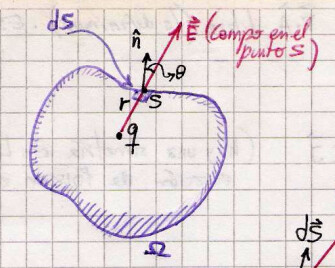
\includegraphics[width=0.35\textwidth]{images/fig_ft1_gauss.pdf}	 
% 	\end{center}
% 	\caption{}
% \end{figure} 




% \bibliographystyle{CBFT-apa-good}	% (uses file "apa-good.bst")
% \bibliography{CBFT.Referencias} % La base de datos bibliográfica

\end{document}

	
% 	\input{FT2.c3}
	
		\documentclass[10pt,oneside]{CBFT_book}
	% Algunos paquetes
	\usepackage{amssymb}
	\usepackage{amsmath}
	\usepackage{graphicx}
% 	\usepackage{libertine}
% 	\usepackage[bold-style=TeX]{unicode-math}
	\usepackage{lipsum}

	\usepackage{natbib}
	\setcitestyle{square}

	\usepackage{polyglossia}
	\setdefaultlanguage{spanish}
	



	\usepackage{CBFT.estilo} % Cargo la hoja de estilo

	% Tipografías
	% \setromanfont[Mapping=tex-text]{Linux Libertine O}
	% \setsansfont[Mapping=tex-text]{DejaVu Sans}
	% \setmonofont[Mapping=tex-text]{DejaVu Sans Mono}

	%===================================================================
	%	DOCUMENTO PROPIAMENTE DICHO
	%===================================================================

\begin{document}

% 
% =================================================================================================
\chapter{El oscilador armónico}
% =================================================================================================

Clásicamente la cosa venía de una partícula sometida a un potencial
\[
	V(x) = \frac{kx^2}{2} \qquad \qquad \omega = \sqrt{\frac{k}{m}}.
\]

Para el oscilador armónico cuántico 1D el hamiltoniano y energía son
\[
	H = \frac{p^2}{2m} + \frac{m\omega^2 x^2}{2} \qquad E = \hbar \omega \left( n + \frac{1}{2} \right)
\]
donde $\omega^2$ es la constante del resorte cuántico.
Este problema puede resolverse usando un nuevo operador $\hat{a}$ (operadores de aniquilación
y creación)
\[
	\hat{a} = \sqrt{\frac{m\omega}{2\hbar}}\left( x + i\frac{p}{m\omega} \right) \qquad \text{con} \quad 
	\hat{a}^\dagger = \sqrt{\frac{m\omega}{2\hbar}}\left( x - i\frac{p}{m\omega} \right)
\]
que es suma de $\hat{x}, \hat{p}$ pero que no es hermítico. Cumple que 
\[
	[a , a^\dagger ] = 1 \qquad a a^\dagger =  \frac{H}{\hbar\omega} -1 \qquad 
	H = \hbar\omega \left( a a^\dagger + \frac{1}{2} \right),
\]
donde se define el operador número $\hat{N}\equiv a^\dagger a$ que al verificar $[\hat{N},\hat{H}]=0$ tienen 
base de 
autoestados en común $\{ \Ket{n} \}$. En efecto 
\[
	\hat{N} \Ket{n} = n\Ket{n} \qquad
	\hat{H} \Ket{n} = \hbar\omega \left( n + \frac{1}{2} \right) \Ket{n}
\]
siendo $n$ el número de cuantos de energía.
Se cumplen además 
\[
	[N,a] = [a^\dagger a,a] = - [ a, a^\dagger a ] = - \left( a^\dagger [a,a] + [a,a^\dagger]a \right) =
	-a
\]
\[
	[N,a^\dagger] = [a^\dagger a, a^\dagger ] = - [a^\dagger , a^\dagger a ] =
	- \left( a^\dagger [a^\dagger,a] + [a^\dagger,a]a^\dagger \right) = a^\dagger
\]

Queremos ver que le  hace $a^\dagger$  a un autoestado $\Ket{n}$ y luego $a$ sobre el mismo.
\[
	N a^\dagger \Ket{n} = ([N, a^\dagger] + a^\dagger N) \Ket{n} =
	a^\dagger \Ket{n} + a^\dagger n \Ket{n} 
\]
\[
	\Hat{N} (a^\dagger\Ket{n}) = (n+1)(a^\dagger\Ket{n})
\]
Entonces, como no hay degeneración y tenemos $N\Ket{n'} = n'\Ket{n'}$ entonces 
\[
	a^\dagger \Ket{n} = c_1 \Ket{n+1},
\]
y procediendo de modo idem para $a\ket{n}$ será
\[
	a \Ket{n} = c_2 \Ket{n-1}
\]
Luego,
\[
	a^\dagger \Ket{n} = c_1 \Ket{n+1} \overbrace{\longrightarrow}^{DC} 
	\Bra{n+1} c_1^* = \Bra{n} a 
\]
\[
	a \Ket{n} = c_2 \Ket{n-1} \overbrace{\longrightarrow}^{DC} \Bra{n-1} c_2^* = \Bra{n} a^\dagger
\]
y entonces 
\[
	\Braket{n|N|n} = n \Braket{n|n} = n =  \Braket{n| a^\dagger a |n} =  \Braket{n-1|c_2^* c_2|n-1} =
	|c_2|^2 \Braket{n-1|n-1}
\]
\[
	n = \Braket{n|aa^\dagger-1|n} = -1 + \Braket{n|aa^\dagger|n} = - 1 + \Braket{n+1|c_1^*c_1|n+1} =
	-1 + |c_1|^2 \Braket{n+1|n+1}
\]
siendo
\[
	|c_2| = \sqrt{n} \qquad |c_1| = \sqrt{n+1} 
\]
\[
	\hat{a}^\dagger \Ket{n} = \sqrt{n+1} \Ket{n+1} \qquad  \hat{a}\Ket{n} = \sqrt{n} \Ket{n-1} 
\]
y entonces de esta forma $\hat{a}^\dagger$ es el operador de creación de cuantos y $\hat{a}$ el de 
aniquilación.
Estos operadores permiten ir saltando de niveles de energía y pasar entre estados definidos estos
por el número de cuantos.
Nótese que $\hat{a}$ es operador de aniquilación cuando actúa sobre kets; sobre bras los crea.

Del producto interno se tiene
\[
	(\Bra{n}a^\dagger)(a\Ket{n}) \geq 0
\]
lo cual conduce a $ n \geq 0 $.

\subsection{El estado fundamental $\Braket{0}$}

\[
	a \Ket{n}  \overbrace{\longrightarrow}^{DC} \Bra{n} a^\dagger
\]
y desde el postulado para productos internos,
\[
	(\Bra{n}a^\dagger)(a\Ket{n}) \geq 0 \quad n \Braket{n|n} \geq 0 \Rightarrow n \geq 0 
\]
entonces $n$ cabalga por los naturales.
Si hacemos 
\[
	a\Ket{n} = \sqrt{n} \Ket{n-1}, \quad  
	a^2 \Ket{n} = \sqrt{n (n-1)} \Ket{n-2} \quad 
	a a^2 \Ket{n} = \sqrt{n (n-1)(n-2)} \Ket{n-3} \; ...
\]
en algún momento (dado que $n\geq 0$) se llega a $\Ket{n=0}$, entonces $E_0 = \hbar\omega/2$ y 
\[
	\Ket{0} \equiv \text{El fundamental}
\]
y no se puede bajar más,
\[
	\hat{a}\Ket{0} = 0.
\]

Por otra parte, con el $\hat{a}^\dagger$ se puede llegar a cualquier estado
\[
	a^\dagger \Ket{0} = \sqrt{1} \Ket{1}, \qquad  a^{\dagger 2} \Ket{0} = \sqrt{1}\sqrt{2} \Ket{2} = 
	\sqrt{1}\sqrt{2}\sqrt{3} \Ket{3}
\]

\begin{figure}[htb]
	\begin{center}
	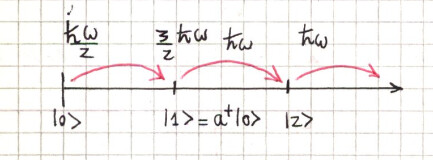
\includegraphics[width=0.6\textwidth]{images/fig_ft2_osc_arm1.jpg}	 
	\end{center}
	\caption{}
\end{figure} 

Se tienen todos los valores de energía a partir de uno solo,
\[
	\frac{{(a^{\dagger})}^n}{\sqrt{n}!} \Ket{0} = \Ket{n} \qquad \qquad 
	E_n = \hbar \omega \left( n + \frac{1}{2} \right)
\]

Las matrices de $\hat{a},\hat{a}^\dagger$ sólo tienen una diagonal corrida de elementoss 
\[
	\Braket{n'|a|n} = \sqrt{n} \Braket{n'|n-1} = \sqrt{n} \delta_{n',n-1}
\]
\[
	\Braket{n'|a^\dagger|n} =  \sqrt{n-1} \Braket{n'|n+1} = \sqrt{n-1} \delta_{n',n+1}
\]
Es decir, que pictóricamente serían algo como
\[
	a^\dagger = \begin{pmatrix}
	0 & \sqrt{1} & 0 & 0 & ... \\
	0 & 	0    & \sqrt{2} & 0 & ... \\
	0 & 	0    & 0 & \sqrt{3} & ... \\
	0 & ... \\
	0 & ... & & & \sqrt{n} \\
	0 & ... & & & 0 
	\end{pmatrix}
\]
y
\[
	a = \begin{pmatrix}
	0 & 0 & & & \\
	\sqrt{1} & 0 & 0 & & ... \\
		0    & \sqrt{2} & 0 & & ... \\
	 	0    & 0 & \sqrt{3} & &... \\
	 ... \\
	 ... & & & \sqrt{n} & 0 \\
	\end{pmatrix}
\]
Los elementos de las matrices
\[
	\Braket{n'|x|n} = \sqrt{\frac{\hbar}{2m\omega}}
	(\sqrt{n}\delta_{n',n-1} + \sqrt{n+1}\delta_{n',n+1})
\]
\[
	\Braket{n'|p|n} = i \sqrt{\frac{\hbar}{2m\omega}}
	(-\sqrt{n}\delta_{n',n-1} + \sqrt{n+1}\delta_{n',n+1})
\]
no pueden ser matrices diagonales porque no conmutan con el hamiltoniano.

También puede verse que 
\[
	\vm{x} = \Braket{n|x|n}= 0 \qquad \vm{p} = \Braket{n|p|n}= 0,
\]
lo cual difiere de lo que esperaríamos clásicamente. Es más, se tienen también
\be
	x^2 = \frac{\hbar}{2 m \omega}( a^2 + a^{\dagger 2} + aa^\dagger + a^\dagger a )
	\label{x2_osc_arm}
\ee
y consecuentemente
\[
	\Braket{0|x^2|0}= \frac{\hbar}{2 m \omega} \qquad 
	\Braket{0|p^2|0}= \frac{\hbar m \omega}{2}
\]
de manera que resulta
\[
	\Braket{(\Delta x)^2}_{\Ket{0}} \Braket{(\Delta p)^2}_{\Ket{0}} = \frac{\hbar^2}{4} 
\]
el estado fundamental es el de incerteza mínima.
Esto es así porque estamos en el fundamental y es un pack gaussiano.

Veamos ahora la forma que tiene la función de onda. A tiempo cero.
Siendo $\Psi_n(x') = \Braket{x'|n}$ quiero evaluar $\Psi_0(x') = \Braket{x'|0}$ y ver que como 
\[
	\Braket{x'|a|0}= 0 
\]
tengo 
\[
	0 = \sqrt{ \frac{m\omega}{2\hbar} } \Braket{x'|x+\frac{ip}{m\omega}|0} =
	\sqrt{ \frac{m\omega}{2\hbar} } \left[ x'\Braket{x'|0} + \frac{i}{m\omega}\Braket{x'|p|0} \right]
\]
\[
	x' \Braket{x'|0} + \frac{i}{m\omega} (-i\hbar) \dpar{}{x} \Braket{x'|0} = 0
\]
entonces 
\[
	x' \Braket{x'|0} = - \frac{\hbar}{m\omega} \dpar{}{x'}\Braket{x'|0} 
\]
\[
	- \int \frac{m\omega}{\hbar} x' dx' = \int \frac{d \Braket{x'|0}}{\Braket{x'|0}} \Rightarrow 
	\Braket{x'|0} = \kappa \euler^{-m\omega x^{'2}/(2\hbar)}
\]
y entonces 
\[
	1 = \int_{-\infty}^{\infty} \Braket{0|x'}\Braket{x'|0} dx' = 
	\int_{-\infty}^{\infty} |\kappa|^2 \euler^{-m\omega x^{'2}/\hbar} dx' =
	|\kappa|^2 \sqrt{\frac{\pi\hbar}{m\omega}} 
\]
\[
	|\kappa| = \left( \frac{m\omega}{\pi\hbar} \right)^{1/2} = \frac{1}{(\pi x_0^2)^{1/4}}
\]
donde usamos el conocido resultado $\int_{-\infty}^\infty \exp( - a x^2) dx = \sqrt{\pi/a}$, llegamos al 
llamado pack 
gaussiano.
\[
	\Braket{x'|0} = \frac{1}{(\pi x_0^2)^{1/4}} \euler^{-\frac{1}{2}\left( x'/x_0 \right)^2}
\]
El estado fundamental tiene incerteza mínima y debe corresponder a un paquete gaussiano.

Se ven que 
\[
	\Braket{x'|1} = \Braket{x'|a^\dagger|0}
\]
y lo escribo en función de $x$ y $p$ que sé cómo operan sobre $x'$. Entonces
\[
	\Braket{x'|1} = \frac{1}{\sqrt{2}x_0} \left( x' - x_0^2 \dtot{}{x'} \right) \Braket{x'|0}
\]
y se puede demostrar que vale
\[
	\Braket{x'|n} = \frac{1}{\pi^{1/4} \sqrt{2^n n!}} \frac{1}{x_0^{n+1/2}} 
	\left( x' - x_0^2 \dtot{}{x'} \right)^n \euler^{-1/2 (x'/x_0)^2}.
\]

Los operadores $a,a^\dagger$ son útiles para la resolución de problemas discretos.
En el oscilador armónico las energías son discretas, hasta el infinito, y están
equiespaciadas $\hbar \omega$.

\notamargen{Esto ya se dijo en otra parte y está descolgado aquí.}
Notemos que $\hat{a}^\dagger$ crea sobre ket y aniquila sobre bra, mientras que $\hat{a}$ aniquila 
sobre ket y crea sobre bra,
\[
	a^\dagger \Ket{n} = \sqrt{n+1} \Ket{n+1} \Rightarrow \Bra{n} a = \Bra{n+1} \sqrt{n+1}
\]
\[
	a \Ket{n} = \sqrt{n} \Ket{n-1} \Rightarrow \Bra{n} a^\dagger = \Bra{n-1} \sqrt{n}
\]

\begin{ejemplo}{\bf Ejercicio 8}

Tiene muchos resultados de la teoría que no repetiré aquí.
Para evaluar $\Braket{m|\hat{x}|n}$ se lo escribe en términos de $a, a^\dagger$, luego se opera.
Vemos que $\Braket{m|\hat{x}|n}$ y $\Braket{m|\hat{p}|n}$ no son diagonales en esta base y que
los elementos diagonales son nulos.

El cálculo de $\Braket{m|\hat{x}^2|n}$ es directo pero engorroso. Se puede ver que usando la
expresión de $x^2$ en términos de $a, a^\dagger$ dada por la \eqref{x2_osc_arm} se puede ver que
vale n
\[
	\Braket{m|\hat{x}^2|n} = \frac{\hbar }{2 m \omega}
	\left[ 
	\sqrt{n(n+1)} \delta_{m,n-2} + \sqrt{(n+1)(n+2)} \delta_{m,n+2} + 2(n+1)\delta_{mn}
	\right]
\]
\[
	\Braket{m|\hat{p}^2|n} = - \frac{m \hbar \omega }{2}
	\left[ 
	-(2n+1) \delta_{mn} + \sqrt{(n+1)(n+2)} \delta_{m,n+2} + \sqrt{n(n-1)}\delta_{m,n-2}
	\right]
\]

Entonces tenemos
\[
	\Braket{n|\hat{p}^2|n} = \frac{m \hbar \omega }{2} ( 2n + 1 )
	\qquad 
	\Braket{n|\hat{x}^2|n} = \frac{\hbar}{2 m \omega} ( 2n + 1 )
\]
y con esto se puede verificar el teorema del virial.
Para autoestados de $H$ se da que 
\[
	(\Delta x)^2 = \vm{x^2} - \vm{x}^2, \qquad 
	(\Delta p)^2 = \vm{p^2} - \vm{p}^2
\]
y usando lo obtenido arriba
\[
	(\Delta x)^2 (\Delta p)^2 = \frac{\hbar^2}{4}(2n+1)^2 \geq \frac{\hbar^2}{4}
\]
y se ve que el signo de igualdad vale para el $n=0$, el fundamental.

La función de onda del fundamental será $\Braket{x'|0}$ y podemos usar que
\[
	\Braket{x'|a|0} = \Braket{x'| \left( x + \frac{i}{m\omega} p \right)|0} 
	\sqrt{\frac{m\omega}{\hbar}} = 0
\]
lo que resulta en
\[
	x' \Braket{x'| 0} + \frac{\hbar}{m\omega} \dpar{}{x} \Braket{x'|0} = 0,
\]
que es una ecuación diferencial para la función de onda 
cuya solución se puede escribir, definiendo $x_0 \equiv \hbar / (m\omega) $,
\[
	\Braket{x|0} = \frac{1}{\hbar^{1/4} \sqrt{x_0}} \euler^{-1/2 (x'/x_0)^2}
\]
una gaussiana centrada en el origen.

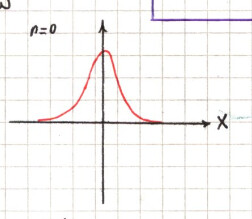
\includegraphics[width=0.35\textwidth]{images/fig_ft2_osc_arm_gaussiana.jpg}

El siguiente estado lo generamos con el operador de creación,
\[
	a^\dagger \Ket{0} = \Ket{1}
\]
de manera que en la pic de abajo podemos ver en la primer fila las funciones de
onda y en la segunda la probabilidad resultante.

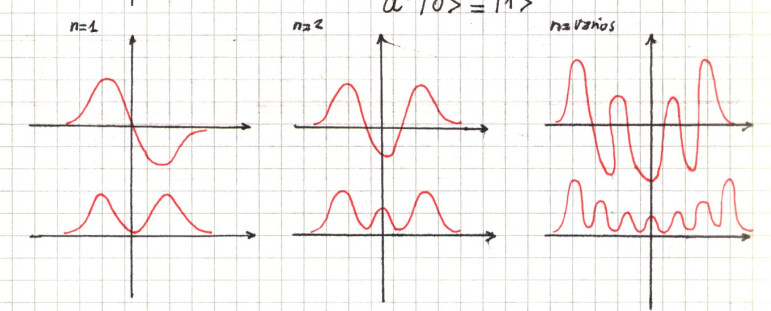
\includegraphics[width=0.9\textwidth]{images/fig_ft2_osc_arm_gaussiana_plancha.jpg}

 
Veamos ahora la evolución temporal en la representación de Heisenberg. Todos los operadores
dependen del tiempo, luego
\[
	\dtot{p}{t} = -\frac{i}{\hbar}[p,H] = -m \omega^2 x \qquad \qquad 
	\dtot{x}{t} = -\frac{i}{\hbar}[x,H] = \frac{p}{m}
\]
y asimismo,
\[
	[p, \frac{p^2}{2m} + \frac{m\omega^2 x^2}{2}] = \frac{m \omega^2}{2} [p,x^2] =
	\frac{m\omega^2}{2}(-2 i \hbar )
\]

Es conveniente hacer una transformación canónica $x,p \to a,a^\dagger$, luego
\[
	\dtot{a}{t} = - i \omega a \qquad \qquad 
	\dtot{a^\dagger}{t} =  i \omega a^\dagger
\]
siendo el conmutador
\[
	[a,H] = \hbar \omega [a,a^\dagger a] = 
	\hbar\omega ( a^\dagger [ a, a ] + [ a, a^\dagger ] a )
\]
con
\[
	a(t) = a(0) \euler^{ - i \omega t } \qquad \qquad 
	a^\dagger(t) = a^\dagger(0) \euler^{ i \omega t }
\]
Poniendo $a,a^\dagger$ en términos de $x, p$ con
\[
	x(t) + i \frac{p(t)}{m\omega} = 
	x(0)\euler^{i\omega t} + i \frac{p(0)}{m\omega}\euler^{-i\omega t}
\]
\[
	x(t) - i \frac{p(t)}{m\omega} = 
	x(0)\euler^{i\omega t} - i \frac{p(0)}{m\omega}\euler^{-i\omega t}
\]
y equating ambas
\[
	x(t) = x(0)\cos(\omega t) + \frac{p(0)}{m\omega} \sin(\omega t)
\]
\[
	p(t) = - m \omega x(0)\sin(\omega t) + p(0) \cos(\omega t).
\]
Esto también se puede calcular con el operador evolución, a través de
\[
	x(t) = \euler^{i H / \hbar t} \: x \: \euler^{-i H / \hbar t},
\]
aunque es un camino mucho más {\it painful}.
Facilitamos un poco con el {\bf lema de Baker-Hausdorff} que dice que
\[
	\euler^{[iG\lambda]} \hat{A} \euler^{-[iG\lambda]} =
	\hat{A} + i \lambda [G,A] + \frac{i^2\lambda^2}{2!}[ G, [G,A ] ] + ... +
	\frac{i^2\lambda^n}{n!} [ G, [ G, [ G, ... [G,A] ] ] ]
\]
con $G$ hermítico y $\lambda$ real.

El primer término es $x$ luego se tienen
\[
	2) \quad [H, x(0)] = - \frac{ i \hbar p(0) }{ m }
\]
\[
	3) \quad [ H, [ H, x(0) ] ] = [ H, -\frac{i \hbar p(0)}{m} ] =
	-[H,p(0)]\frac{i\hbar}{m} = \hbar^2 m x(0)
\]
\[
	4) \quad [ H, [ H, [ H,x(0)] ] ] = [ H, -i \hbar^2 x(0) ] = [ H, x(0) ] \hbar^2
\]
amasando todo esto se llega a
\[
	x(t) = x(0) + \left[ \frac{p(0)}{m} \right] t - \frac{1}{2!}t^2\omega^2 x(0) -
	\frac{1}{3!} \frac{t^3\omega^2 p(0)}{m} + ...
\]
y con un poco de buena vista se pueden identificar en esta serie las expresiones de 
\[
	\sin(\omega t) = \sum_{n=0}^\infty \frac{(\omega t)^{2n+1}}{(2n+1)!} (-1)^n
\]
\[
	\cos(\omega t) = \sum_{n=0}^\infty \frac{(\omega t)^{2n}}{(2n)!} (-1)^n
\]
 
Faltaría ver la evolución de los valores medios $\Braket{n|x(t)|n}=0$ y 
$\Braket{n|p(t)|n} = 0 $, pero se quedan en cero por ser estacionarios [?].
Las oscilaciones solamente aparecerán en estados que son combinación lineal de autoestados
de energía.
 
\end{ejemplo}


\subsection{Interferencia en experimento de Young}

Consideremos la situación depicted en la figura bajo estas líneas, que es reminiscente de la del
experimento de Young aunque la fuente no necesariamente es de luz.

\begin{figure}[h]
	\begin{center}
	\includegraphics[width=0.6\textwidth]{images/teo2_6.pdf}
	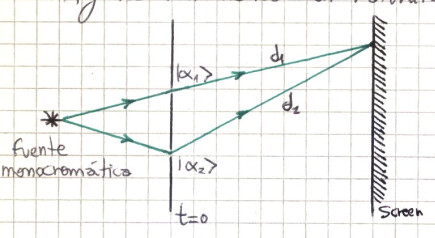
\includegraphics[width=0.6\textwidth]{images/fig_ft2_young_analogous.jpg}
	\end{center}
	\caption{}
\end{figure} 

Uso $\hat{H}$ de partículas libres y que $\Ket{\a}$ es el generado por la fuente.
Suponemos que en $t=0$ al pasar por las aberturas se da
\[
	\frac{1}{2} \Ket{\alpha} = \Ket{\alpha_1} = \Ket{\alpha_2}
\]
y luego para $t>0$ se tiene 
\[
	\Ket{\tilde{\alpha_1}} = \euler^{ -i H t /\hbar } \Ket{\alpha_1} =
		\euler^{ -i E_\alpha t /\hbar } \Ket{\alpha_1}	
\]
\[
	\Ket{\tilde{\alpha_2}} = \euler^{ -i E_\alpha t /\hbar } \Ket{\alpha_2}	
\]

En la pantalla debe verse la interferencia de los dos estados solapados. La diferencia de caminos
es la que genera la interferencia, y usando que los tiempos son $t_i = d_i/v$ se da
\[
	\Ket{\tilde{\alpha}} = \Ket{\tilde{\alpha_1}} + \Ket{\tilde{\alpha_2}} =
		\euler^{ -i E_\alpha \frac{d_1}{v} /\hbar } \Ket{\alpha_1} +
		\euler^{ -i E_\alpha \frac{d_2}{v} /\hbar } \Ket{\alpha_2}	
\]
\[
	\Ket{\tilde{\alpha}} = \frac{1}{2} \euler^{ -i E_\alpha \frac{d_1}{v} /\hbar } 
		\left[ 1 + \euler^{ -i E_\alpha \frac{d_2-d_1}{v} /\hbar } \right] \Ket{\alpha_1}
\]
y si definimos
\[
	\beta=E_\alpha \frac{d_2-d_1}{v} /\hbar,
\]
resulta entonces
\[
	\Braket{\tilde{\alpha}|\tilde{\alpha}} = 
	\frac{1}{4}| 1 +  \euler^{ -i E_\alpha \frac{d_2-d_1}{v} /\hbar } |^2 =
		\frac{1}{4}( (1+\cos\beta)^2 + \sin^2\beta ) =
			\frac{1}{2} + \frac{1}{2}\cos\left( \beta \right).
\]
Esto sería la intensidad si de radiación electromagnética se tratase.

Al partir el estado $\Ket{\alpha_1} $ y volver a unirlo en $\Ket{\alpha_1} + \Ket{\alpha_2}$ vemos una 
intensidad que depende de la diferencia de camino.

\subsection{Cambio de cero del potencial}

Consideramos una partícula sometida a potencial externo.
El potencial es una maquinación matemática conveniente para el concepto más físico de fuerza.
Es un caso particular de cambio de gauge.


En mecánica clásica la física de un problema no se ve afectada por un cambio de gauge.
Si movemos el cero de potencial, la situación física es la misma.
Veamos qué sucede en mecánica cuántica.
\[
	\Ket{\alpha,t,t_0} = \euler^{ -i (p^2/2m + V(x))(t-t_0)/\hbar} \Ket{\alpha,t_0}
\]
\[
	\Ket{\tilde{\alpha},t,t_0} = \euler^{ -i (p^2/2m + V(x) + V_0)(t-t_0)/\hbar} \Ket{\alpha,t_0}
\]
\[
	\Ket{\tilde{\alpha},t,t_0} = \euler^{ -i V_0(t-t_0)/2 }\Ket{\alpha,t,t_0}
\]
y entonces vemos que $\Ket{\tilde{\alpha},t}$ y $\Ket{\alpha,t}$ difieren en una fase, de manera que los 
valores de expectación (las magnitudes físicas) no cambian (con $V_0$ constante).
El efecto fue meter una fase.

Si el potencial es tal que $V_0 = V_0(t)$ entonces
\[
	\Ket{\tilde{\a},t,t_0} = \euler^{ -i \int_{t_1}^{t_2} V(t) dt } \Ket{\a,t,t_0}.
\]


\begin{figure}[htb]
	\begin{center}
	\includegraphics[width=0.6\textwidth]{images/teo2_7.pdf}
	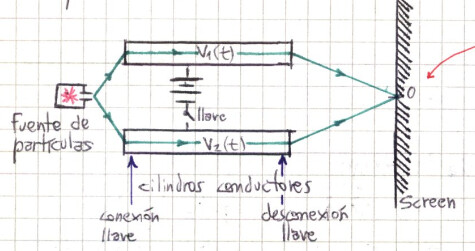
\includegraphics[width=0.6\textwidth]{images/fig_ft2_cero_potential.jpg}
	\end{center}
	\caption{}
\end{figure} 

Consideremos ahora un experimento ideal (pensado). 
Dentro de los cilindros hay campo nulo siempre. Se varia el $V$ abriendo y cerrando la 
llave a la entrada y a la salida; se varía el cero de potencial pero no el campo.
Se cambia la fase de las partículas inferiores respecto de las superiores, entonces habrá 
interferencia en $O$.

Clásicamente no hay variación, pero cuánticamente
\[
	\Delta \text{fase} = -\frac{i}{\hbar}\euler \int _{t_1}^{t_2} V_1(t) - V_2(t) dt = 
	-\frac{i}{\hbar}\euler \Delta V
\]
Notemos que con el límite $\hbar \to 0$ el efecto desaparece [no será el otro límite o hay algo mal?].

Lo que realmente cuenta es la diferencia de potencial $\Delta V$, la cual sí tiene sentido 
físico porque es independiente de la medida y porque pueden escribirse los campos en función de aquella.

\begin{ejemplo}{\bf Caso gravitatorio}
 
Clásicamente la masa inercial con la gravitatoria se cancelan,
\[
	m \ddot{x} = - m \nabla \phi_g
\]
y esto lleva a que la aceleración sea $g$, luego la gravedad es algo geométrico porque no depende de la masa.
Cuánticamente,
\[
	\left( -\frac{\hbar^2}{2m}\nabla^2 + m \phi_g \right) \psi = i \hbar \dpar{\psi}{t}
\]
la masa no se simplifica. Aún así 
\[
	\dtot[2]{}{t} \vm{x} = - g.
\]

 
\end{ejemplo}


\begin{ejemplo}{\bf Experimento Colella/Overhauser/Werner}

Esto viene de un artículo de Physical Review Letters.
Se utilizan partículas neutras: neutrones.
Consideramos el setup siguiente
 
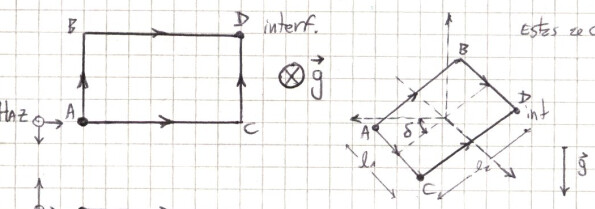
\includegraphics[width=0.6\textwidth]{images/fig_ft2_colella.jpg} 

La diferencia de altura es $\Delta h = \ell_2 \sin \delta $ pero en la derecha se tiene que
$\bar{BD}$ está a mayor altura que $\bar{AC}$ que está más baja.
Luego, la longitud de onda Compton
\[
	v = \frac{p}{m} = \frac{1}{m} \frac{2m\hbar}{\lambda} = \frac{\hbar}{m\lambda_c}
\]
y entonces
\[
	\euler^{ - i/\hbar m g \ell_x \sin \delta \ell_1/v }
\]
de manera que
\[
	\phi_{ABC} - \phi_{ACD} = 
	\frac{ m^2 g \ell_1 \ell_2 \lambda_c \sin \delta }{\hbar^2}
\]
se tiene un fenómeno puramente cuántico (aparece $\hbar$) y depende de la masa.
  
\end{ejemplo}

\subsection{Caso del EM y la invariancia de gauge}

Recordemos algunos resultados del electromagnetismo.
\[
	E = - \Nabla\phi - \frac{1}{c}\dpar{\vb{A}}{t}
\]
Si el cuadrivector de momento es $p^\mu = (E/c, \vb p)$ y el de cuadri potencial es 
$A^\mu =(\phi,\vb A)$ se veía que el reemplazo
\[
	p^\mu \to p^\mu - \frac{e}{c} A^\mu
\]
era covariante.
Luego, el hamiltoniano covariante era
\be
	H = \frac{1}{2m} \left( \vb{p} - \frac{\euler\vb{A}}{c}\right)^2 + \euler \phi 
	\label{ham_cov_em}
\ee

En el formalismo de Heisenberg
\[
	\dtot{H}{t} = \frac{1}{i\hbar}[x_i,H] = \frac{p_i - e A_i / c}{m}
\]
puesto que $p$ y $A$ no conmutan. Los momentos son justamente $\pi_i = p_i - e/c A_i$.
Luego,
\[
	[ p_i, p_j ] = 0 \qquad 
	[ \pi_i , \pi_j ] = \frac{i\hbar e}{c} \epsilon_{i l k}B_k
\]

La invariancia de gauge hace que
\[
	\phi \to \phi - \frac{1}{c}\dpar{\Lambda}{t} \qquad \quad 
	\vb A \to \vb A + \nabla \Lambda
\]
que es un cambio que deja los campos $\vb E, \vb B$ invariantes. Si la función $\Lambda \neq \Lambda(\vb x)$
entonces el cambio es como un cambio de cero del potencial, pues 
\[
	\phi \to \phi + \lambda(t) \qquad \vb A \to \vb A.
\]

La mecánica cuántica incluye la invariancia de gauge de modo que los valroes de expectación, que es lo
físico, no se alteran.
El cambio de fase implicado por la transformación de gauge no pasa a los valores de expectación.

Considerando la versión operacional del hamiltoniano \eqref{ham_cov_em} y la ecuación de Schrödinger,
\[
	H \Ket{\a,t_0,t} = i \hbar \dpar{}{t} \Ket{\a,t_0,t}
\]
Ahora quiero hacer una transformación de gauge para ver si obtengo las mismas mediciones.
Reemplazando los operadores $p$ y $A$ por los transformados según el cambio de gauge se obtiene
(luego veremos la justificación, creámoslo por ahora)
\[
	\Ket{\tilde{\a},t_0,t} = \euler^{ i e \Lambda(x,t)/(\hbar c)}\Ket{\a,t_0,t} 
\]
y a esta fase la denominaresmos $\hat{g}(x,t)$ (un operador?) luego, la transformación de gauge implica
\[
	\Braket{\a|x|\a} \to  \Braket{\tilde{\a}|x|\tilde{\a}} = \Braket{\a|g^\dagger x g|\a}
\]
y como conmutan,
\[
	\Braket{\a|x g^\dagger g|\a} = \Braket{\a|x|\a}
\]
donde el último paso es por la unitariedad. Luego, el $x$ no cambia por una transformación de gauge.

Veamos qué le pasa al momento conjugado $\pi$, teniendo en cuenta que el momento lineal mecánico $p$ no varía
pero sí el potencial $A$, i.e.
\[
	\Braket{\a|\pi|\a} \to  \Braket{\tilde{\a}|\tilde{\pi}|\tilde{\a}} =
	\Braket{\tilde{\a}| p - \frac{e\tilde{A}}{c} |\tilde{\a}}
\]
Luego,
\[
	\Braket{\tilde{\a}| g^\dagger \left( p - \frac{e {A}}{c} - \frac{e}{c} \nabla\Lambda \right) g |\tilde{\a}}
\]
donde hay que recordar que $p$ tiene metida la derivada respecto de $x$ y $A, \Lambda$ son sólo dependientes
de $x,t$ y conmutan con $g(x,t)$. Se ve que resulta todo el operador $p - e/c A$ y la transformación cumple
además que $\Braket{\a|\a} =  \Braket{\tilde{\a}|\tilde{\a}} $ de forma que se ha demostrado lo que se
propusiera antes.
Tenemos
\begin{multline}
	\left[ \frac{1}{2m}\left( p - \frac{e {A}}{c} - \frac{e \nabla\Lambda}{c} \right)^2 +
	e \: \phi - \frac{e}{c} \dpar{\Lambda}{t} \right] 
	\euler^{i e \Lambda/ (\hbar c)} \Ket{\a,t_0,t} = \\
	\euler^{i e \Lambda/ (\hbar c)} 
	\left( - \frac{e}{c} \dpar{\Lambda}{t} + i \hbar \dpar{}{t} \right) \Ket{\a,t_0,t}
\end{multline}
donde se ve que valen varias cosas
\[
	g g^\dagger \left( p - \frac{e {A}}{c} - \frac{e \nabla\Lambda}{c} \right) g = 
	g \left( p - \frac{e {A}}{c}  \right)
\]
Con esto debería ser suficiente para confirmar el resultado [confirmarlo].
La mecánica cuántica es, entonces, invaraitne de gauge al igual que lo que sucedía en mecánica clásica.

\begin{ejemplo}{\bf Experimento de Aharonov y Bohm}

Vemos en la figura que las partículas no interactúan con el campo $\vb B$ y el circulito es un solenoide
infinito. Hay campo magnético dentro pero es nula afuera. Tengo, no obstante, potencial $\vb A$ en todas
partes.

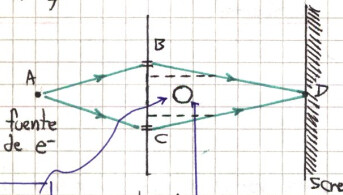
\includegraphics[width=0.5\textwidth]{images/fig_ft2_aharonov_bohm.jpg} 

Luego, resulta que hay interferencia en $D$ sin campo $\vb B$ por al diferencia de fases originada 
por el potencial $\vb A$.

La fase es
\[
	- \frac{i}{\hbar} \int_{t_1}^{t_2} \left( - \frac{e}{c} \dtot{\vb x}{t} \cdot \vb A\right) dt=
	\frac{i e}{\hbar c} \int_{x_1}^{x_2} \vb A \cdot d\vb x.
\]
Recordemos que el lagrangiano de la situación\footnote{Hay un lagrangiano para cada momento, como para ahora
que me estoy tomando una copa de vino.} [?]
\[
	\Lag = \frac{m}{2} \Dtot{\vb x}{t}^2 + \frac{e}{c} \dtot{\vb x}{t}\cdot\vb A
\]

Quisiéramos ver cuál es la diferencia de fase entre los dos caminos ABD y ACD, que será
\[
	\frac{ie}{\hbar c} \left( \int_{ABD} \vb A\cdot d\vb x - \int_{ACD} \vb A\cdot d\vb x \right) =
	\frac{ie}{\hbar c} \left( \int_{ABD} \vb A\cdot d\vb x + \int_{DCA} \vb A\cdot d\vb x \right) =
	\frac{ie}{\hbar c}  \int_{cerrada} \vb A\cdot d\vb x
\]
que conduce a
\[
	\frac{ie}{\hbar c}  \int_{cerrada} \rotorm{A} \: d\vb S = \frac{ie}{\hbar c} \phi_B \neq 0
\]
es decir que hay efecto de interferencia. Notemos que el rotor sigue siendo invariante de gauge [?].

Físicamente el campo $\vb B$ no interactúa con el ahz de partículas, con lo cual parecería una interacción
del potencial con las partículas.
 
\end{ejemplo}


% =================================================================================================
\section{El propagador}
% =================================================================================================

Físicamente representa la proababilidad de transición entre autoestados por el paso del tiempo,
$ \Ket{x'}_{t_0} \longrightarrow \Ket{x''}_t$.
La idea es que si en $t=0$ el estado del sistema es un autoestado $\Ket{x'}$, interesará ver cuál
es la probabilidad de hallarse en $\Ket{x''}$ en $t$.
El propagador se define como:
\[
	\Braket{x''|\euler^{-iH(t-t_0)/\hbar}|x'} \equiv K(x',t; x, t_0),
\]
pero veamos cómo aparece en el curso de un cálculo.
Consideremos
\[
	\Braket{x''| \alpha,t_0,t} = 
	\Braket{x''|\euler^{-iH(t-t_0)/\hbar}|\alpha,t_0},
\]
\[
	\Braket{x''| \alpha,t_0,t} = 
	\int dx' \Braket{x''|\euler^{-iH(t-t_0)/\hbar}|x'}\Braket{x'|\alpha,t_0}.
\]
Entonces la función de onda se escribe
\[
	\Psi_{\alpha}(x'',t) = \int dx' K(x'',t; x',t) \Psi_{\alpha}(x',t).
\]

Podemos pensar que el propagador lleva o ``propaga'' la función de onda desde $t_0$ a $t$. 
% Es como la función de Green.
Se puede escribir:
\[
	K(x',t; x, t_0) = \sum_{a'} \Braket{x''|a'} \Braket{a'|x'} \euler^{-iE_a(t-t_0)/\hbar}
\]
y metemos un observable $\hat{A}$ donde $[A,H]=0$ y $A\Ket{a'}=a\Ket{a'}$.

El propagador depende del potencial, pero no de la función de onda inicial. Se debe cumplir que:
\[
	\lim_{t\to t_0} K(x',t; x, t_0) = \delta^3(x''-x')
\]
\[
	K(x'',t; x, t_0) = \Braket{x''|\euler^{-iH(t-t_0)/\hbar}|a'} \Braket{a'|x'} =
		\sum_{a'} \Psi_{\Ket{a'}}(x'',t)\Braket{a'|x'}
\]
\[
	K(x'',t; x, t_0) = \sum_{a'} c_{a'}(x')\Psi_{\Ket{a'}}(x'',t)
\]
y entonces el propagador es una función de Green que satisface 
\[
	\left( -\frac{\hbar^2}{2m}\nabla^2 +V(x'') - i\hbar\dpar{}{t} \right)K(x',t; x, t_0) =
		- i\hbar \delta^3(x''-x') \delta(t-t_0)
\]
con $K(x'',t;x',t_0)=0 $ si $t<0$ que es la condición de contorno.

\begin{ejemplo}{\bf El propagador de la partícula libre}

Escribimos el propagador como integral en el momento de acuerdo con
\begin{multline*}
 	K(x'',t; x, t_0) = \int dp' \Braket{x''|\euler^{-ip^2(t-t_0)/2m\hbar}|p'} \Braket{p'|x'} = \\
 	\int dp' \euler^{-ip'^{2}(t-t_0)/2m\hbar} \Braket{x''|p'} \Braket{p'|x'} = \\
 	\frac{1}{2\pi\hbar} \int dp' \euler^{-ip'^{2}(t-t_0)/2m\hbar} \euler^{-ip'(x'-x'')/\hbar}
\end{multline*}
y entonces el propagador de una partícula libre es
\[
	K(x'',t; x, t_0) = \sqrt{ \frac{m}{2\pi i\hbar(t-t_0)} } \euler^{i\frac{m(x''-x')^2}{2\hbar(t-t_0)}}
\]

También se puede escribir el propagador en la representación de Heisenberg,
\[
	\Braket{x''|\euler^{-iH(t-t_0)/\hbar}|x'} = 
	\Bra{x''}\euler^{-iHt/\hbar} \euler^{iHt_0/\hbar}\Ket{x'} = \Braket{x'',t|x',t_0}
\]
y entonces
\[
	K(x'',t;x',t_0) = \Braket{x'',t | x',t_0},
\]
el propagador es la probabilidad de transición de pasar entre puntos $x'$ y $x''$.

El propagador tienq que cumplir la propiedad del operador evolución, esto es la propiedad de composición 
(como el $U(t,t_0)$), es decir:
\[
	K(x'',t; x, t_0) = K(x'',t; x, t_1)K(x'',t_1; x, t_0) \qquad t>t_1>t_0,
\] 
lo cual se puede ver explícitamente considerando
\[
	\Braket{x''| \euler^{-i H/\hbar ( t - t_1 + t_1 -t_0 )}|x'} =
	\int dx_1 \Braket{ x''| \euler^{- i H (t-t_1) /\hbar } | x_1 }  
		\Braket{ x_1| \euler^{- i H (t_1-t_0) /\hbar } | x' }
\]
de lo cual vemos
\[
	\Braket{x''| \euler^{-i H/\hbar ( t - t_1 + t_1 -t_0 )}|x'} =
	\Braket{x'',t|x_1,t_1}  \Braket{x_1,t_1|x',t_0}.
\]

\end{ejemplo}


% =================================================================================================
\section{Integrales de camino de Feynmann}
% =================================================================================================

Consideramos una partícula yendo de $(x_1,t_1)$ a $(x_N,t_N)$. Dividimos el tiempo 
\[
	\delta t = \frac{t_N-t_1}{(N-1)}
\]
y queremos ver la amplitud de transición desde el estado 1 al $N$. Es decir,
% En mecánica clásica yo iba por un solo camino; el que minimizaba la acción $S$.
% En mecánica cuántica tengo infinitos caminos que interfieren entre sí.
\begin{figure}[htb]
	\begin{center}
	\includegraphics[width=0.5\textwidth]{images/teo2_8.pdf} 
	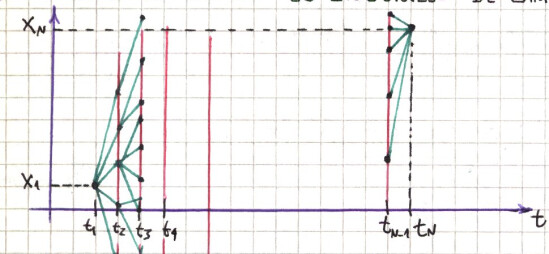
\includegraphics[width=0.5\textwidth]{images/fig_ft2_feynmann_path_int.jpg}
	\end{center}
	\caption{}
\end{figure} 
\begin{multline*}
	\braket{x_N,t_N|x_1,t_1} = \int dx_{N-1}\int dx_{N-2} \; ... \\
	... \int dx_2 \Braket{x_N,t_N|x_{N-1},t_{N-1}} ...\Braket{x_2,t_2|x_1,t_1}
\end{multline*}

Se puede pensar como que estamos sumando sobre todos los posibles caminos entre 
$(x_1,t_1)$ y $(x_N,t_N)$ fijos. 
En mecánica clásica teníamos un solo camino, el que minimizaba la acción $S$
\[
	\delta \int_{t_1}^{t_2} \Lag dt = \delta S = 0
\]
pero en cambio en mecánica cuántica todos los caminos aportan (e interfieren entre sí). 
En un libro de Dirac, Feymann lee 
\[
	\Braket{x_2,t_2|x_1,t_1} \; \text{corresponde a} \; \euler^{i\int_{t_1}^{t_2}\Lag/\hbar \: dt}
\]
y entonces propone
\[
	\Braket{x_2,t_2|x_1,t_1} \approx \sum_{\text{caminos}} 
	\euler^{ i\int_{t_1}^{t_2} \Lag_{\text{clasico}}(x,\dot{x}) /\hbar \: dt}
\]

Definiremos
\[
	S_{(n,n-1)}\equiv \int_{t_{n-1}}^{t_n}\Lag(x,\dot{x}) dt
\]
Luego para considerar la suma sobre todos los segmentillos a lo largo de un camino tendremos
\[
	\prod_{n=2}^N \euler^{i/\hbar S(n,n-1)} = \euler^{i/\hbar \prod_{n=2}^N S(n,n-1)} = \euler^{iS(N,1)/\hbar}
\]
y hay que considerar TODOS los posibles caminos (cada uno de los cuales aporta un $\euler^{iS/\hbar}$) 
\[
	\propto \sum_{caminos} \euler^{i/\hbar S(N,1)} 
\]
cuando $\hbar \to 0$ las trayectorias contribuyen con una cantidad que oscila loca y violentamente. 
Tienden a la cancelación para caminos aledaños. Por el $\hbar \sim 0$ la fase es grande y entonces
se cancelan. Esto no ocurre cerca del camino (real) que cumple 
\[
	\delta S(N,1) = 0
\]
Para trayectorias cercanas la $\Delta fase$ no es grande y hay interferencia constructiva.
Para un $\delta t$ infinitesimal cualquier trayectoria puede verse como una línea recta y es 
\[
	\Braket{x_n,t_n|x_{n-1},t_{n-1}} = N \euler^{iS(n,n-1)/\hbar}
\]
\begin{multline*}
	S(n,n-1) = \int_{t_{n-1}}^{t_n} \left( \frac{m}{2}\dot{x}^2 - V(x)\right) dt \\ 
	\approx \int_{t_{n-1}}^{t_n} \left( \frac{m}{2} \frac{(x_n-x_{n-1})^2}{\delta t^2} - 
	V\left(\frac{x_n+x_{n-1}}{2}\right)\right)  dt 
\end{multline*}
donde la última expresión es a orden 1 en el tiempo y en la posición (pues $\delta t \sim 0$).
\begin{figure}[htb]
	\begin{center}
	\includegraphics[width=0.45\textwidth]{images/teo2_9.pdf}
	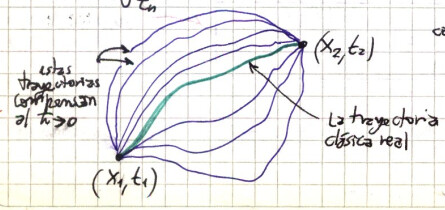
\includegraphics[width=0.45\textwidth]{images/fig_ft2_feynmann_path_int_2.jpg}
	\end{center}
	\caption{}
\end{figure} 

Consideremos, por ejemplo, una partícula libre, entonces $V=0$ de modo que resolviendo 
se obtiene
\[
	\Braket{x_n,t_n|x_{n-1},t_{n-1}} = N \euler^{i m (x_n - x_{n-1})^2/2\hbar\delta t},
\]
que no es otra cosa que el propagador de una partícula libre. La normalización $N$ se puede
evaluar tomando
\[
	\lim_{\Delta t \to 0} N \euler^{i m (x_n - x_{n-1})^2/2\hbar\delta t} = \delta( x_n - x_{n-1} )
\]
y usando el resultado de que
\[
	\lim_{\Delta t \to 0} \sqrt{\frac{m}{2\pi i \hbar \Delta t}}
	\euler^{ i m y^2/(2\hbar) \delta t} = \delta(y),
\]
se obtiene
\[
	N = \sqrt{\frac{m}{2\pi i \hbar \Delta t}}.
\]
La normalización no depende del potencial $V$ en el lagrangiano.

Veamos cómo se comporta para un $\Delta t$ finito será 
\begin{multline*}
	\Braket{x_n,t_n|x_1,t_1}  = 
	\lim_{N\to\infty} \left(\frac{m}{i2\pi\hbar\delta t}\right)^{(N-1)/2}
	\int dx_{n-1}\int dx_{n-2} \; ... \\
	\int dx_2 \prod_{n=2}^N \euler^{i S(n,n-1)/\hbar}
\end{multline*}
y defino una integral de medida dada por toda la sucesión de integraciones anidadas
en la anterior exprsión, nomenclada como $\int_{x_1}^{x_n} D[x(t)]$ de suerte que
resulta
\[
	\Braket{x_n,t_n|x_1,t_1}  = 
	\int_{x_1}^{x_n} D[x(t)] \euler^{i \int _{t_1}^{t_n} \Lag(x,\dot{x})/\hbar} dt
\]
siendo esta última la integral de camino de Feynmann.
La acción es una fase aquí. Las integrales on los caminos cuánticos y por ello esto tiene
toda la información del sistema cuántico.

En base a las integrales de camino, Feynamn desarrolla una formulación equivalente de la 
mecánica cuántica que utiliza los conceptos de:
\begin{enumerate}
 \item Superposición
 \item Composición de la transición
 \item Límite clásico con $\hbar \to 0$
\end{enumerate}

Estas integrales contienen toda la información del sistema cuántico, aunque no sea sencillo extraerla.

\begin{ejemplo}{\bf Integral de camino para partícula libre}

Para una partícula libre la expresión se puede evaluar, 
\[
	\lim_{N\to\infty} \left(\frac{m}{i2\pi\hbar\delta t}\right)^{(N-1)/2}
	\int dx_{n-1}\int dx_{n-2} \; ... 
	\int dx_2 \prod_{n=2}^N \euler^{ \frac{ i m}{2\hbar} \frac{(x_n - x_{n-1})}{\Delta t} \Delta t}
\]
\[
	\euler^{ \frac{ i m }{2 \hbar \Delta t } } \sum_{j=2}^N \: ( x_j - x_{j-1} )^2
\]
\[
	( x_N - x_{N-1} )^1 + (x_{N-1} - x_{N-2})^2 + ... + ()^2 + ()^2
\]
Al final del día esta cuenta da
\[
	\lim_{N\to\infty} \left( \frac{ m }{2 \pi i \hbar (N-1) \delta t} \right)^{\frac{1}{2}}
	\euler^{ i m (x_N - x_{N-1})^2 /( 2(N-1)\hbar \delta t )}
\]
donde el límite fue $(N-1)\Delta t \to (t_N -t_1)$.
 
\end{ejemplo}


Consideremos un propagador de $(x',0) \to (x',t)$
\[
	G(t) = \int dx' K(x',t ; x', 0) = \int dx' \Braket{x'|\euler^{-i Ht/\hbar}|x'}
\]
\begin{multline*}
	G(t) = \sum_{a'} \int dx' \Braket{x'|\euler^{-i Ht/\hbar}|a'}\Braket{a'|x'} = \\
		\sum_{a'} \euler^{-i E_{a'}t/\hbar} \int dx' \Braket{x'|a'}\Braket{a'|x' } 
\end{multline*}
\[
	G(t) = \sum_{a'} \euler^{-i E_{a'}t/\hbar} \int dx' |\Braket{x'|a'}|^2 = 
	\sum_{a'} \euler^{-i E_{a'}t/\hbar} 
\]
que es reminiscencia de la función de partición de mecánica estadística. Tomando Laplace-Fourier 
\[
	\tilde{G}(E) = -i \int dE \frac{G(t)}{\hbar} \euler^{i E t/\hbar} = \sum_{a'} \frac{1}{E-E_{a'}}
\]
y el espectro de autoenergías son los polos de $\tilde{G}(E)$.
O, dicho de otra manera, los polos de la función $G$ propagador integrada en $x$ y luego de
haberle hecho Fourier, son la autoenergías.


La expresión 
\[
	\Braket{x,t|x_1,t_1} \equiv \text{Integral de camino de Feynmann}
\]
satisface la ecuación de Schrödinger y es una alternativa a la formulación de la cuántica usual.


% \bibliographystyle{CBFT-apa-good}	% (uses file "apa-good.bst")
% \bibliography{CBFT.Referencias} % La base de datos bibliográfica

\end{document}

	
% 		\documentclass[10pt,oneside]{CBFT_book}
	% Algunos paquetes
	\usepackage{amssymb}
	\usepackage{amsmath}
	\usepackage{graphicx}
% 	\usepackage{libertine}
% 	\usepackage[bold-style=TeX]{unicode-math}
	\usepackage{lipsum}

	\usepackage{natbib}
	\setcitestyle{square}

	\usepackage{polyglossia}
	\setdefaultlanguage{spanish}
	



	\usepackage{CBFT.estilo} % Cargo la hoja de estilo

	% Tipografías
	% \setromanfont[Mapping=tex-text]{Linux Libertine O}
	% \setsansfont[Mapping=tex-text]{DejaVu Sans}
	% \setmonofont[Mapping=tex-text]{DejaVu Sans Mono}

	%===================================================================
	%	DOCUMENTO PROPIAMENTE DICHO
	%===================================================================

\begin{document}





% \bibliographystyle{CBFT-apa-good}	% (uses file "apa-good.bst")
% \bibliography{CBFT.Referencias} % La base de datos bibliográfica

\end{document}

	
		\documentclass[10pt,oneside]{CBFT_book}
	% Algunos paquetes
	\usepackage{amssymb}
	\usepackage{amsmath}
	\usepackage{graphicx}
% 	\usepackage{libertine}
% 	\usepackage[bold-style=TeX]{unicode-math}
	\usepackage{lipsum}

	\usepackage{natbib}
	\setcitestyle{square}

	\usepackage{polyglossia}
	\setdefaultlanguage{spanish}
	

	\everymath{\displaystyle}

	\usepackage{CBFT.estilo} % Cargo la hoja de estilo

	% Tipografías
	% \setromanfont[Mapping=tex-text]{Linux Libertine O}
	% \setsansfont[Mapping=tex-text]{DejaVu Sans}
	% \setmonofont[Mapping=tex-text]{DejaVu Sans Mono}

	%===================================================================
	%	DOCUMENTO PROPIAMENTE DICHO
	%===================================================================

\begin{document}

% =================================================================================================
\chapter{Introducción al momento angular (rotaciones)}
% =================================================================================================

El operador $\hat{L}$ será el encargado de realizar las rotaciones. Por el álgebra visto en la mecánica 
clásica sabemos que, dado un vector \vb{v} y una matriz ortogonal $R$ se tiene
\[
	\vb{v}' = R \vb{v} \qquad \text{con} \quad |\vb{v}'|=|\vb{v}|
\]
y 
\[
	|\vb{v}|^2 = V^t V = (V^t R^t) (R V) \qquad \text{pues} \quad R^tR=RR^t = \mathbb{1}
\]
puesto que es una matriz ortogonal.
Una matriz ortogonal tiene tres parámetros independientes.
Luego se cumplen 
\begin{itemize}
 \item Clausura 
 \[
	(R_1R_2)(R_1R_2)^t = R_1R_2R_2^tR_1^t = \mathbb{1}
\]
\item El producto de dos matrices ortogonales es otra matriz ortogonal (aquella que cumple $R^rR=\mathbb{1}$).
Asociatividad
\[
	R_1(R_2R_3) = (R_1R_2)R_3
\]
\item Existencia de identidad
\[
	R \: \mathbb{1} = \mathbb{1}R = R
\]
\item Existencia de inversa
\[
	R \: R^{-1} = R^{-1}R = \mathbb{1} \qquad \text{con}\; R^{-1}\equiv R^t
\]
\end{itemize}

Esto define un grupo de matrices ortogonales que realiza rotaciones y se denomina $SO(3)$.
Las rotaciones son un grupo respecto a la multiplicación.

\subsection{No conmutatividad de las rotaciones clásicas}

Las rotaciones finitas no conmutan. Luego, el grupo de las rotaciones será un grupo abeliano
\[
	R_z(\varphi) = \begin{pmatrix}
	\cos(\varphi) & -\sin(\varphi) & 0 \\
	\sin(\varphi) & \cos(\varphi) & 0 \\
	0 & 0 & 1
	\end{pmatrix}
\]
\[
	R_x(\varphi) = \begin{pmatrix}
	1 & 0 & 0 \\
	0 & \cos(\varphi) & -\sin(\varphi) \\
	0 & \sin(\varphi) & \cos(\varphi)
	\end{pmatrix}
\]
\[
	R_y(\varphi) = \begin{pmatrix}
	\cos(\varphi) & 0 & \sin(\varphi) \\
	0 & 1 & 0 \\
	-\sin(\varphi) & 0 & \cos(\varphi)
	\end{pmatrix}
\]

\begin{figure}[!htb]
	\begin{center}
	\includegraphics[width=0.4\textwidth]{images/teo2_10.pdf}
	\end{center}
	\caption{}
\end{figure} 

Si reemplazamos $\cos(\epsilon) \approx 1 - \epsilon^2/2$ y $\sin(\epsilon) \approx \epsilon$ hasta orden dos.
Se puede ver que las rotaciones, en torno a ejes diferentes, sólo conmutan a orden uno $(\epsilon)$ de manera 
que una rotación infinitesimal $d\varphi$ conmuta pero una rotación finita $\varphi$ no lo hace.

En efecto, hasta orden 2 se tienen 
\[
	R_z(\epsilon) = \begin{pmatrix}
	1 - \epsilon^2/2 & - \epsilon  & 0 \\
	\epsilon & 1 - \epsilon^2/2 & 0 \\
	0 & 0 & 1
	\end{pmatrix}
\]
\[
	R_x(\epsilon) = \begin{pmatrix}
	1 & 0 & 0 \\
	0 & 1 - \epsilon^2/2 & -\epsilon \\
	0 & \epsilon & 1 - \epsilon^2/2
	\end{pmatrix}
\]
\[
	R_y(\epsilon) = \begin{pmatrix}
	1 - \epsilon^2/2 & 0 & \epsilon \\
	0 & 1 & 0 \\
	-\epsilon & 0 & 1 - \epsilon^2/2
	\end{pmatrix}
\]

Entonces, se ve que
\[
	R_x(\epsilon) R_y(\epsilon) - R_y(\epsilon) R_x(\epsilon) = 
	\begin{pmatrix}
	0 & -\epsilon^2  & 0 \\
	\epsilon^2 & 0 & 0 \\
	0 & 0 & 0
	\end{pmatrix}	
\]
o bien
\[
	[ R_x(\epsilon), R_y(\epsilon) ] =  R_z(\epsilon) - \mathbb{1}
\]

Como el conmutador es diferente de cero el grupo de las rotaciones es un grupo no abeliano.
La velocidad angular se define $\d\omega/dt$ de modo que eso justifica que los vectores
velocidad angular puedan sumarse en mecánica.
Esto es lo que sucedía en el caso clásico. Veamos ahora qué le pasa a los kets ante rotaciones.

% =================================================================================================
\section{Rotaciones cuánticas}
% =================================================================================================

Para las rotaciones cuánticas suponemos la existencia de un operador $D_R$ que las realiza, que
convierte $ \Ket{\a} \to \Ket{\a}_R $ con $ \Ket{\a}_R = D(R) \Ket{\a} $ postulándose una forma del
tipo 
\[
	D(\hat{n},d\phi) = \mathbb{1} - i \frac{\vb{J}\cdot\hat{n}}{\hbar}d\phi,
\]
para una rotación infinitesimal o bien
\[
	D(\hat{n},\theta) = \lim_{N\to\infty} \left( 1 - \frac{i J_z \theta}{\hbar N} \right)^N =
	\euler^{-i \vb{J}\cdot\hat{n}/\hbar \theta},
\]
para rotación finita. 
$\hat{D}$ es, como se dijo, el operador de las rotaciones y $\hat{J}$ es un momento angular 
general. Se postula de esta forma para que $\hat{D}$ cumpla las mismas propiedades que $R$ y la 
misma relación de conmutación (lo cual los hace pertenecer al mismo álgebra)
\[
	R_x R_y - R_y R_x = R_z (\epsilon^2) - \mathbb{1}
\]
\[
	D(\hat{x},\epsilon) D(\hat{y},\epsilon) - D(\hat{y},\epsilon) D(\hat{x},\epsilon) =
	D(\hat{z},\epsilon^2) - D(\mathbb{1})
\]
de modo que la cuenta lleva a  
\[
	J_x J_y - J_y J_x = i \hbar J_z
\]
la cual generalizando se llega a 
\[
	[J_i,J_j] = i \hbar \epsilon_{ijk} J_k
\]
que son las relaciones de conmutación generales para momento angular $\hat{J}$.
Esto vale para cualquier rotación, lo cual es más amplio que si es solo $L$, el momento angular.

\begin{ejemplo}{\bf Operador de rotación para partículas de spin 1/2}
 
Para sistemas de spín $1/2$ es 
\[
	D(\hat{n},\phi) \equiv \euler^{-i/\hbar \vb{S}\cdot\hat{n} }
\] 
El efecto de la rotación se asocia a 
\[
	_R\Braket{\a|S_x|\a}_R = \Braket{ \a | \euler^{i S_z \phi /\hbar} 
	\: S_x \: \euler^{-i S_z \phi /\hbar}  | \a }
\]
una cosa que podemos considerar como un operador y los kets fijos en el tiempo.
La base de autoestados de $S_z$ es 
\[
	S_z\Ket{+} = \frac{\hbar}{2}\Ket{+} \qquad \qquad 
	S_z\Ket{-} = -\frac{\hbar}{2}\Ket{-}
\]
los operadores $S_x, S_y, S_z$ tienen sus expresiones usuales y evaluando resulta
\[
	D^\dagger \: S_x \: D =
	\frac{\hbar}{2} 
	\left[
	( \KB{+}{-} + \KB{-}{+} ) \cos\phi + i ( \KB{+}{-} - \KB{-}{+}  )\sin \phi 
	\right]
\]
que es como si el vector $S_x$ se transformase como lo haría un vector. En efecto,
se tiene
\[
	S_x \qquad \to \text{rotación} \to \qquad S_x \cos\phi - S_y \sin\phi
\]
\[
	S_y \qquad \to \text{rotación} \to \qquad S_y \cos\phi + S_x \sin\phi
\]
pero 
\[
	S_z \qquad \to \text{rotación} \to \qquad S_z
\]
lo cual se demuestra por conmutación en la expresión del operador.
 
Se puede ver que ante rotaciones cuánticas $D(\hat{n},\phi)$ los valores de expectación transforman como 
vectores
\[
	\begin{pmatrix} \Braket{S_x'} \\ \Braket{S_y'} \\ \Braket{S_z'}	\end{pmatrix} =	\begin{pmatrix} 
	\\
	 R(\hat{x},\phi) \\
	 \\
	\end{pmatrix}\begin{pmatrix} \Braket{S_x} \\ \Braket{S_y} \\ \Braket{S_z} \end{pmatrix}
\]

En general $\vb{J} = (J_x, J_y, J_z)$ se transforma como vector y entonces $\hat{J}$ es un operador vectorial.
Consideremos un estado de un sistema de spín $1/2$,
\[
	\Ket{\alpha} = \Braket{+|\alpha}\Ket{+} + \Braket{-|\alpha}\Ket{-}
\]
\[
	D(\hat{z},\phi)\Ket{\alpha} = \euler^{-iS_z\phi/\hbar}\Braket{+|\alpha}\Ket{+} +
		\euler^{-iS_z\phi/\hbar} \Braket{-|\alpha}\Ket{-}
\]
\[
	D(\hat{z},\phi)\Ket{\alpha} = \Braket{+|\alpha} \euler^{-i\phi/2} \Ket{+} +
		\euler^{i\phi/2} \Braket{-|\alpha}\Ket{-}
\]
Haciendo una rotación de $\phi=2\pi$ (cosa que debiera dejar al ket incólume) se tiene 
\[
	D(\hat{z},2\pi) \Ket{\alpha} = - \Braket{+|\alpha}\Ket{+} - \Braket{-|\alpha}\Ket{-} = -\Ket{\alpha}
\]

Luego, esto es una muestra del carácter no-clásico del spin; una vuelta completa le cambia el signo al ket 
pero notemos cuidadosamente que el valor de expectación -- que es algo físico -- no varía. Esto muestra que 
el ket no puede tener sentido físico.

Se observó en 1975 que el patrón de interferencia se altera con el $-\Ket{\a}$ de manera que tiene 
importancia ese signo en el ket.

En la picture se esquematiza. Hay necutrones a la izquierda y un campo magnético $\vb B$ delante de la
parted. Se ve en la interferencia que llega con el signo cambiado; le hacen dar una vuelta completa
al spin.

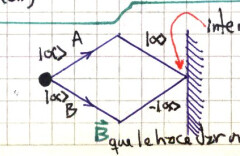
\includegraphics[width=0.20\textwidth]{images/fig_ft2_spin12_rotaciones_experimento.jpg}

\end{ejemplo}

\subsection{Angulos de Euler}

Se define una serie de rotaciones 
\[
	1.\; R_{z}(\alpha) \qquad 2.\; R_{y'}(\beta)\qquad 3.\; R_{z'}(\gamma)
\]
lo cual equivale a
\[
	R(\alpha,\beta,\gamma) = R_{z'}(\gamma) R_{y'}(\beta) R_{z}(\alpha)
\]
\notamargen{Recordemos que en general no se sabe cómo acctúan los operadores sobre un
estado general sino sobre autoestados.}
\[
	\euler^{-i J_{z'}\gamma/\hbar} \euler^{-i J_{y'}\beta/\hbar}  \euler^{-i J_z\alpha/\hbar} 
	\Ket{\psi}
\]
\begin{figure}[!htb]
	\begin{center}
	\includegraphics[width=0.4\textwidth]{images/teo2_11.pdf}
	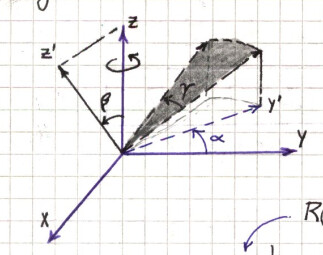
\includegraphics[width=0.4\textwidth]{images/fig_ft2_convencion_euler_angles.jpg}
	\end{center}
	\caption{Los ángulos de Euler son una caracterización de una rotación general en 3D.}
\end{figure} 
Pero desconozco cómo operar en los ejes móviles $z',y'$ así que buscaré escribir las rotaciones 
de manera que se pueda hacer la cuenta, refiriéndolas a ejes fijos.
\[
	R_{y'}(\beta) = R_{z}(\alpha) R_{y}(\beta) R_{z}^{-1}(\alpha) 
\]
\[
	R_{z'}(\gamma) = R_{y'}(\beta) R_{z}(\gamma) R_{y'}^{-1}(\beta) 
\]
siendo estas dos expresiones generales (puede probarse)
\[
	R(\alpha,\beta,\gamma) =
	R_{y'}(\beta) R_{z}(\gamma) \underbrace{R_{y'}^{-1}(\beta)R_{y'}(\beta)}_{\mathbb{1}}R_{z}(\alpha) 
\]
\[
	R(\alpha,\beta,\gamma) =
	R_{z}(\alpha) R_{y}(\beta) R_{z}^{-1}(\alpha) R_{z}(\gamma) R_{z}(\alpha)  
\]
donde las que son sobre el mismo eje conmutan y entonces,
\[
	R(\alpha,\beta,\gamma) = R_{z}(\alpha) R_{y}(\beta) R_{z}(\gamma).
\]
Rotación equivalente a [1] pero para ejes fijos, puesto que en mecánica cuántica sabemos rotar en torno a 
ejes fijos.

Los ángulos de Euler son la caracterización de una rotación general en 3D.
Entonces nuestra rotación en 3D cuántica será:
\[
	D(\alpha,\beta,\gamma) = D_z(\alpha) D_y(\beta) D_z(\gamma)  =
	\euler^{-i J_z\alpha/\hbar} \euler^{-i J_y\beta/\hbar} \euler^{-i J_z\gamma/\hbar}
\]

\subsection{Autoestados y autovalores de J}

Partimos de 
\[
	[J_i, J_j] =  i\hbar \epsilon_{ijR}J_R
\]
y
\[
	J^2 = J^2_x + J^2_y + J^2_z, \qquad  [J^2,J] = 0
\]
siendo la última muy importante y probándose por evaluación directa. Lleva a 
\[
	[J^2,J_i^n] = 0 \qquad \text{con} \; i=x,y,z \;\; n\in\mathbb{N}
\]

Se eligen $J^2, J_z$ como observables que conmutan 
\[
	J^2 \Ket{a,b} = a\Ket{a,b} \qquad \qquad J_z \Ket{a,b} = b\Ket{a,b}
\]
siendo $a$ autovalor de $J^2$ y $b$ de $J_z$.

Definiremos los operadores de subida y de bajada
\[
	J_{\pm} \equiv J_x \pm J_y
\]
que verifican 
\[
	[ J_+, J_- ] = 2\hbar J_z \qquad [ J_z, J_\pm]= \pm \hbar J_{\pm} \qquad [J_{\pm}, J^2 ] = 0
\]
Entonces se tiene 
\[
	J^2( J_\pm \Ket{a,b}) = J_\pm J^2 \Ket{a,b} = a J_\pm \Ket{a,b} \longrightarrow 
		J_\pm \Ket{a,b} = \Box \Ket{a,b}
\]
\[
	(J_zJ_\pm - J_\pm J_z) \Ket{a,b} = \pm\hbar J_\pm \Ket{a,b}
\]
\[
	J_z (J_\pm \Ket{a,b}) = (b\pm\hbar)(J_\pm \Ket{a,b}) \longrightarrow 
		J_\pm \Ket{a,b} = \boxdot \Ket{a,b\pm\hbar}
\]
\[
	J_{\pm} \Ket{a,b} = c_{\pm} \Ket{a,b\pm\hbar}
\]
\[
	J_+\Ket{a,b} = c_+\Ket{a,b+\hbar} \;\qquad\; J_-\Ket{a,b} =  c_- \Ket{a,b-\hbar}
\]
sube el $J_z$ en una unidad de $\hbar$ o bien baja el $J_z$ en una unidad de $\hbar$.
\[
	J_+J_- = J_x^2 + iJ_yJ_x - iJ_xJ_y + J_y^2 , \qquad J_-J_+ = J_x^2 - iJ_yJ_x + iJ_xJ_y + J_y^2
\]
\[
	J^2 = J_z^2 + \frac{1}{2}(J_+J_- + J_-J_+ ) , \qquad 
		J^2 - J_z^2 = \frac{1}{2}(J_+J_+^\dagger + J_+^\dagger J_+ )
\]
\[
	\Braket{a,b|J^2 - J^2_z|a,b} =  1/2 \Braket{a,b|J_+J_+^\dagger + J_+^\dagger J_+|a,b}
\]
\[
	(a-b^2)\Braket{a,b|a,b} = 1/2 \left[ \Braket{a,b|J_+J_+^\dagger|a,b} + 
		\Bra{a,b|J_+^\dagger} J_+\Ket{a,b} \right] 
\]
\[
	(a-b^2)\Braket{a,b|a,b} = |J_+^\dagger\Ket{a,b}|^2 \geq 0, \qquad \Rightarrow a \geq b^2
\]
hay cota para $b$.
\[
	J_+ \Ket{a,b_M} = 0
\]
Como no puede seguir subiendo debe dar el ket nulo 
\[
	J_-J_+ \Ket{a,b_M} = 0
\]
pero
\[
	J_-J_+ = J^2_x + J^2_y + i[J_x, J_y]  = J^2 - J^2_z - \hbar J_z
\]
\[
	( J^2 - J^2_z  -\hbar J_z) \Ket{a,b_M}  = 0	
\]
\[
	( a - b_M^2 - \hbar b_M ) \Ket{a,b_M}  = 0	
\]
\[
	a = b_M ( b_M -\hbar )
\]
\[
	J_- \Ket{a,b_m} = 0
\]
y como no puede seguir bajando debe dar el ket nulo
\[
	J_+J_- \Ket{a,b_m} = 0
\]
\[
	J_+J_- =  J^2 - J^2_z + \hbar J_z
\]
\[
	( J^2 - J^2_z + \hbar J_z) \Ket{a,b_m} = ( a - b_m^2 + \hbar b_m) \Ket{a,b_m} = 0
\]
\[
	b_M( b_M + \hbar ) = b_m( b_m -\hbar )
\]
tiene solución $b_M-b_m = -\hbar$ si $b_M + b_m \neq 0$ 
pero esto es absurdo de manera que $b_M = b_m$.
Entonces
\[
	-b_m = b_M  \qquad \Rightarrow \qquad -b_M \leq b \leq b_M
\]

Luego,
\[
	\Ket{a,b_m} \longrightarrow \Ket{a,b_M}
\]
y como $J_+$ sube de a un $\hbar$ será
\[
	b_M = b_m + n\hbar
\]
y entonces
\[
	b_M = \frac{n\hbar}{2} = \frac{n}{2} \hbar = j \hbar
\]
y se da que $j$ es entero o semientero.

Definiremos 
\[
	b_M \equiv j \hbar \qquad a \equiv j (j+1) \hbar^2 \qquad -j\hbar \leq b \leq j\hbar
\]
pero como $b/\hbar = m$
\[
	b_M \equiv j \hbar \qquad a \equiv j (j+1) \hbar^2 \qquad -j \leq m \leq j
\]
\[
	m = (-j,-j+1,-j+2,...,j-1,j) \qquad 2j+1 \text{valores de} \; m
\]
\[
	J^2 \Ket{j,m} = j( j+1 )\hbar^2\Ket{j,m} \qquad J_z \Ket{j,m} = m \hbar \Ket{j,m}
\]

\subsection{La normalización de $J_\pm$}

\[
	J_+\Ket{j,m} = c_+ \Ket{j,m+1} \qquad \qquad J_-^\dagger = J_+
\]
\[
	\Braket{j,m|J_-J_+|j,m} = \Braket{j,m|J_+^\dagger J_+|j,m} = |c_+|^2
\]
\[
	\Braket{j,m|J^2 - J_z^2 - \hbar J_z|j,m} = j(j+1)\hbar^2 - m^2\hbar^2 -\hbar^2 m = |c_+|^2
\]
\[
	c_+ = \hbar\sqrt{j(j+1)-m(m+1)} = \hbar \sqrt{(j-m)(j+m+1)}
\]
\[
	\Braket{j,m|J_+J_-|j,m} = \Braket{j,m|J_-^\dagger J_-|j,m} = |c_-|^2
\]
\[
	= j(j+1)\hbar^2 - m^2\hbar^2 + m\hbar^2 = |c_-|^2
\]
\[
	c_- = \hbar\sqrt{j(j+1)-m(m-1)} = \hbar \sqrt{(j+m)(j-m+1)}
\]
\[
	J_+ \Ket{j,m} = \hbar \sqrt{(j-m)(j+m+1)}\Ket{j,m+1} \qquad 
	J_- \Ket{j,m} = \hbar \sqrt{(j+m)(j-m+1)}\Ket{j,m-1}
\]

\subsection{Elementos de matriz de $J^2, J_z, J_+$}

Asumiendo normalización de $\Ket{j,m}$ se tiene 
\[
	\Braket{j',m'|J^2|j,m} = j(j+1)\hbar^2 \delta_{jj'} \delta_{m' m}
\]
\[
	\Braket{j',m'|J_z|j,m} = m \hbar \delta_{jj'} \delta_{m' m}
\]

\subsection{Elementos de matriz de $\mathcal{D}(R)$}

Ahora queremos ver cual es la forma de los elementos de matriz de $\mathcal{D}(R)$
\[
	\mathcal{D}(R) = \euler^{i \vb{J}\cdot\vec{n}\phi/\hbar}
\]
siendo que $\mathcal{D}(R)$ tiene por efecto rotar el sistema físico.
Lo primero que hay que notar es que 
\[
	\Braket{j',m'|\mathcal{D}(R)|j,m}  \propto \delta_{jj'}
\]
porque $[J^2,J_i]=0$ y entonces $[J^2,J_i^n]=0$ y 
\[
	\mathcal{D}(R) = f(J_i) \; \longrightarrow \; [ J^2, \mathcal{D}(R) ] = 0
\]
y 
\[
	\mathcal{D}^{(j)}_{m' m} =  \Braket{j,m'|\euler^{i \vb{J}\cdot\vec{n}\phi/\hbar}|j,m} 
\]
es una matriz para cada $j$ fijo con $\{ (2j+1)\times(2j+1)=\text{dimensión}\}$
\[
	\mathcal{D}(R)\Ket{j,m} = \sum_{m'} \ket{j,m'}\Braket{j,m'|\euler^{i \vb{J}\cdot\vec{n}\phi/\hbar}|j,m} 
	= \sum_{m'} \mathcal{D}^{(j)}_{m' m}(R) \Ket{j,m'} 
\]
pero las rotaciones no cambian el $j$, $\mathcal{D}(R)$ conecta estados con la misma $j$ y $\mathcal{D}(R) 
\in (2j+1)\times(2j+1)$ 
\[
	\mathcal{D}(R)\Ket{j,m} = \sum_{m'} \mathcal{D}^{(j)}_{m' m}(R) \Ket{j,m'} 
\]

La matriz de $\mathcal{D}(R)$ (no caracterizada por un único $j$) puede ponerse en forma diagonal por bloques:
\[
\begin{matrix} \qquad j' \quad j'' \quad j''' \end{matrix}
\]
\[
	\mathcal{D}(R) = \begin{pmatrix}
	\; \Box & 0 & 0 & \\
	\; 0 & \Box & 0 & \\
	\; 0 & 0 & \Box & \\
	\; & & & \vdots
	\end{pmatrix} \begin{matrix} j' \\ j'' \\ j'''\\ \\ \end{matrix}
\]
con cada bloque de $(2j+1)\times(2j+1)$ , pero siendo cada bloque irreducible. Las matrices de rotación con 
$j$ fijo forman un grupo. $\mathcal{D}_{m'm}^{(j)}(R)$ son los elementillos de la matriz.
\[
	\Ket{j,m} \underbrace{\longrightarrow}_{\text{Rotación}} \mathcal{D}(R)\Ket{j,m} =
	 \sum_{m'} \mathcal{D}^{(j)}_{m' m}(R) \Ket{j,m'} 
\]
donde el $\mathcal{D}^{(j)}_{m' m}(R)$ es la amplitud de hallar al $\Ket{j,m}$ rotado en $\Ket{j,m'}$

\subsection{Forma explícita del operador $\mathcal{D}(R)$}

Los ángulos de Euler permitieron caracterizar la rotación más general. Entonces 
\[
	\mathcal{D}^{(j)}_{m' m} = 
	\Braket{j,m'|\euler^{-iJ_z\alpha/\hbar} \euler^{-iJ_y\beta/\hbar} \euler^{-iJ_z\gamma/\hbar} |j,m}
\]
\[
	\mathcal{D}^{(j)}_{m' m} = \euler^{-i(-m'\alpha + m\gamma)}
	\underbrace{\Braket{j,m'| \euler^{-iJ_y\beta/\hbar}  |j,m}}_{d_{m'm}^{(j)}}
\]
siendo el primer factor una fase.
En los $d_{m'm}^{(j)}$ está la dificultad de la cuenta.

% =================================================================================================
\section{Formalismo de spinores de Pauli}
% =================================================================================================

Apropiado para trabajar con sistemas de spín $1/2$. Estos sistemas son casos particulares de momento angular,
\[
	j = 1/2 \qquad m=-\frac{1}{2},+\frac{1}{2}
\]
y se definen los spinores $\chi_\pm$ como
\[
	\Ket{+} \equiv  \begin{pmatrix} 1 \\ 0  \end{pmatrix} \equiv  \chi_+ \qquad \qquad
	\Ket{-} \equiv  \begin{pmatrix} 0 \\ 1  \end{pmatrix} \equiv  \chi_-
\]
\[
	\Ket{\alpha} = \begin{pmatrix}   \Braket{+|\alpha} \\ \Braket{-|\alpha}  \end{pmatrix}
\]
\[
	\Bra{\alpha} = \begin{pmatrix}  \; \Braket{+|\alpha} \quad \Braket{-|\alpha} \;  \end{pmatrix}
\]

Para spín $1/2$ podemos tomar $\vb{J} = \vb{S}$ por la analogía de las relaciones de conmutación.
A su vez 
\[
	\vb{S} = \frac{\hbar}{2} \vec{\sigma} \qquad \text{con} \qquad \vec{\sigma} \equiv 
	\begin{pmatrix} \; \sigma_x, \sigma_y, \sigma_z \; \end{pmatrix}
\]
que es una especie de vector 
\[
	\vec{\sigma}  =
	\begin{bmatrix}
	 \begin{pmatrix} 0 & 1 \\ 1 & 0 \end{pmatrix}, \begin{pmatrix} 0 & -i \\ i & 0 \end{pmatrix},
	 \begin{pmatrix} 1 & 0 \\ 0 & -1 \end{pmatrix} 
	\end{bmatrix}
\]
Luego esta equivalencia provee expresión de los operadores $S_i$ en términos de matrices de $2\times 2$, así:
\[
	\frac{i}{2}[ J_- - J_+] = J_y = S_y = \frac{\hbar}{2} \sigma_y
\]
siendo que los $J_y$ y $S_y$ actúan sobre kets y el $\sigma$ sobre spinores.

Las matrices de Pauli cumplen las propiedades básicas siguientes 
\[
	\sigma^2_i = \mathbb{1} \qquad \sigma_i^\dagger = \sigma_i
\]
\[
	[ \sigma_, \sigma_j ] = i2\varepsilon_{ijR}\sigma_R \qquad \{\sigma_, \sigma_j \}= \delta_{ij}
\]
\[
	\sigma_i^n = \begin{cases} \mathbb{1} \quad n \; \text{par} \\ \sigma_i \quad n \; \text{impar} 
\end{cases}
\]
\[
	\Ket{+} \equiv \Ket{j=1/2 , m = 1/2} \qquad \Ket{-} \equiv \Ket{j=1/2 , m = -1/2} 
\]
\[
	(\vec{\sigma}\cdot\vb{a})(\vec{\sigma}\cdot\vb{b}) = 
		(\vb{a}\cdot\vb{b}) + i \vec{\sigma}\cdot(\vb{a}\times\vb{b})
\]

\subsection{Aplicación a las rotaciones}

\[
	\mathcal{D}(\hat{n},\phi) = \euler^{-i \vb{J}\cdot\hat{n}\phi/\hbar} = \euler^{-i\vec{\sigma}\cdot\hat{n}\phi/2}
\]
pero 
\[
	(\vec{\sigma}\cdot\hat{n})^n = \begin{cases}
	                                \vec{\sigma}\cdot\hat{n} \qquad n \; \text{impar} \\
	                                \mathbb{1} \qquad \quad \; n \; \text{par} 
	                               \end{cases}
\]
\[
	\euler^{-i\vec{\sigma}\cdot\hat{n}\phi/2} = 1 - i\vec{\sigma}\cdot\hat{n} \:\frac{\phi}{2} - 
	\frac{1}{2!} (\vec{\sigma}\cdot\hat{n})^2\left(\frac{\phi}{2}\right)^2 + 
	\frac{i}{3!} (\vec{\sigma}\cdot\hat{n})^3\left(\frac{\phi}{2}\right)^3 - ...
\]
\[
	\mathcal{D}(\hat{n},\phi) = \euler^{-i\vec{\sigma}\cdot\hat{n}\phi/2} =
	\mathbb{1}\cos\left(\frac{\phi}{2}\right) - i\vec{\sigma}\cdot\hat{n}\sin\left(\frac{\phi}{2}\right)
\]
es el operador de rotación para sistemas de spin $1/2$ (donde $\mathbb{1} \in 2\times 2$). Con esta expresión podemos 
evaluar 
$d^{j=1/2}_{m'm}(\beta)$
\[
	d^{1/2}(\beta) = \begin{pmatrix}
	     \cos(\beta/2) & -\sin(\beta/2)\\
	     \sin(\beta/2) & \cos(\beta/2)
	    \end{pmatrix}
\]
donde hemos usado los resultados 
\[
	\cos(x) = \sum_{n=0}^\infty \frac{(x)^{2n+1}}{(2n+1)!}(-1)^n \qquad 
		\sin(x) = \sum_{n=0}^\infty \frac{(x)^{2n}}{(2n)!}(-1)^n
\]

En el caso general el operador de rotación para sistemas de spin $1/2$ lucirá:
\[
	\begin{matrix} \qquad\qquad \Ket{+} \qquad\qquad\qquad\qquad \Ket{-} \end{matrix}
\]
\[
	\mathcal{D}^{j=1/2} (\alpha,\beta,\gamma) = \begin{pmatrix}
	        \euler^{-\frac{i}{2}(\alpha + \gamma)} \cos\left(\frac{\beta}{2}\right) & 
			- \euler^{-\frac{i}{2}(\alpha - \gamma)} \sin\left(\frac{\beta}{2}\right) \\
	        \euler^{-\frac{i}{2}(\gamma -\alpha )} \sin\left(\frac{\beta}{2}\right) & 
			\euler^{\frac{i}{2}(\alpha + \gamma)} \cos\left(\frac{\beta}{2}\right)
	       \end{pmatrix} 
	       \begin{matrix} \Ket{+} \\ \\  \Ket{-} \end{matrix}
\]

\subsection{Ejemplo}

\[
	d^{1/2}(\pi/2) = \begin{pmatrix}
	                  \sqrt{2}/2 & -\sqrt{2}/2 \\
	                  \sqrt{2}/2 & \sqrt{2}/2
	                 \end{pmatrix}
\]
de manera que 
\[
	d^{1/2}(\pi/2)\chi_{+} = \frac{\sqrt{2}}{2}\begin{pmatrix} 1 & -1 \\  1 & 1 \end{pmatrix}
	                                           \begin{pmatrix}  1 \\ 0  \end{pmatrix} 
				= \frac{\sqrt{2}}{2} \begin{pmatrix}  1 \\ 1 \end{pmatrix} 
\]
\[
	d^{1/2}(\pi/2)\chi_{+} = \frac{\sqrt{2}}{2} (\chi_+ + \chi_- )  = \frac{1}{2} \left( \Ket{+} + \Ket{-} \right)
\]
\[
	d^{1/2}(\pi/2)\chi_{+} = \Ket{S_x ; + }
\]
Este resultado es intuitivamente lógico.


\subsection{Rotaciones en sistemas con $j=1$}

Ahora tenemos 
\[
	j=1 \qquad m = -1,0,1
\]
recordando $J_y$ en términos de escaleras
\[
	J_y = \frac{J_+ - J_i}{2i}
\]
de modo que 
\[
	\begin{matrix} \quad \Ket{1\;1} \quad \Ket{1\;0} \quad \Ket{1\;-\kern-1mm 1} \end{matrix}
\]
\[
	J_y = \frac{i\hbar}{\sqrt{2}} \begin{pmatrix}
	                               \quad 0 & \quad -1 \quad & 0 \quad \\
	                               \quad 1 & \quad 0 \quad & -1 \quad \\
	                               \quad 0 & \quad 1 \quad & 0 \quad
	                              \end{pmatrix} 
	     \begin{matrix}  \Ket{1\;1} \\ \Ket{1\;0} \\ \Ket{1\;-\kern-1mm 1} \end{matrix}
\]
\[
	\euler^{-i\frac{J_y}{\hbar}\beta} = 1 + -\frac{J_y}{\hbar}\beta + 
		(-i)^2\left(\frac{J_y}{\hbar}\beta\right)^2\frac{1}{2!} + 
		(-i)^3\left(\frac{J_y}{\hbar}\beta\right)^3\frac{1}{3!} + ...
\]
\[
	\euler^{-i\frac{J_y}{\hbar}\beta} = 1 - \frac{J_y}{\hbar}\beta -
		\frac{1}{2!} \left(\frac{J_y}{\hbar}\beta\right)^2 -
		\frac{i}{3!}\left(\frac{J_y}{\hbar}\beta\right)^3 + ...
\]
\[
	\left( \frac{J_y}{\hbar} \right)^n = \begin{cases}
	                                      \left( \frac{J_y}{\hbar} \right) \quad n \; \text{impar} \\
	                                      \left( \frac{J_y}{\hbar} \right)^2 \quad n \; \text{par}
	                                     \end{cases}
\]
\[
	\euler^{-i\frac{J_y}{\hbar}\beta} = 1 -  \left( \frac{J_y}{\hbar} \right)^2 (1-\cos(\beta)) -
	i \left( \frac{J_y}{\hbar} \right) \sin(\beta)  = d^{j=1}(\beta)
\]
acá lo vemos como operador (es notación), $d_{m'm}^{j=1}(\beta)$ simboliza la matriz
\[
	\begin{matrix} \Ket{1\;1} \qquad\qquad\quad \Ket{1\;0} \qquad\qquad \Ket{1\;-\kern-1mm 1} \end{matrix}
\]
\[
	d^{j=1}(\beta) =
	\begin{pmatrix}
	\displaystyle \frac{1}{2}( 1 + \cos(\beta)) & -\frac{1}{\sqrt{2}}\sin(\beta) & \frac{1}{2}( 1 - 
\cos(\beta) ) \\
	\displaystyle{\frac{1}{\sqrt{2}}\sin(\beta)} & \cos(\beta) & -\frac{1}{\sqrt{2}}\sin(\beta) \\
	\displaystyle{\frac{1}{2}(1 - \cos(\beta))} & \frac{1}{\sqrt{2}}\sin(\beta) & \frac{1}{2}  ( 1 + 
\cos(\beta) )
	\end{pmatrix} \begin{matrix} \Ket{1\;1} \\ \\ \Ket{1\;0} \\ \\ \Ket{1\;-\kern-1mm 1} \end{matrix}
\]

% =================================================================================================
\section{Momento angular orbital}
% =================================================================================================

\[
	\vb{L} = \vb{x} \times \vb{p}
\]
verifica el álgebra de $\vb{J}$,
\[
	[ L_i, L_j ] = i\hbar \epsilon_{ijR} L_R \qquad L_i = \epsilon_{ijk}x_jp_k
\]
\[
	L_z = xp_y - yp_x
\]
Consideremos ahora una rotación en torno a $z$, en un $\delta\phi$,
\[
	\left( 1 - \frac{iL_z\delta\phi}{\hbar} \right) \Ket{x',y',z'} =
	1 - \frac{iP_y}{\hbar}(x\delta\phi) + \frac{iP_x}{\hbar}(y\delta\phi) \Ket{x',y',z'}
\]
\[
	= \left[ 1 - \frac{i}{\hbar}\left( P_y x\delta\phi - P_x y\delta\phi \right)\right] \Ket{x',y',z'}
\]
esto es una traslación en $\hat{x},\hat{y}$,
\[
	(1-i\frac{L_z}{\hbar}\delta\phi) \Ket{x',y',z'} = \Ket{x'-y'\delta\phi,y'+x'\delta\phi,z'}
\]

Esta traslación es debida a una rotación infinitesimal en $\delta\phi$ torno a $z$ entonces genera las 
rotaciones clásicas en torno a $z$.
\[
	\Psi_\alpha(\vb{x}') = \Braket{x',y',z'|\alpha} \underbrace{\longrightarrow}_{\text{Rotamos en z}}
	\Braket{x',y',z'|1-\frac{iL_z\delta\phi}{\hbar}|\alpha} = \Braket{x'+y'\delta\phi,y'-x'\delta\phi,z'|\alpha}
\]
y en coordenadas esféricas,
\[
	\Psi_\alpha(\vb{x}') = \Braket{r,\theta,\phi|\alpha} 
	\underbrace{\longrightarrow}_{\text{Rotamos en z}} \Braket{r,\theta,\phi-\delta\phi|\alpha}
\]

Podemos hallar una expresión para $L_z$ en esféricas:
\[
	\Braket{r,\theta,\varphi|1-\frac{L_z\delta\phi}{\hbar}|\alpha} \approx
	\Braket{\phi|\alpha} -\dpar{}{\phi}\Braket{\phi|\alpha}\delta\phi
\]
identificamos 
\[
	\Braket{\vb{r}|-\frac{iL_z}{\hbar}|\alpha} = -\dpar{}{\phi}\Braket{\vb{r}|\alpha}
\]
\[
	L_z =  -i\hbar\dpar{}{\phi}
\]
operador $L_z$ en esféricas.

Esta construcción usa que 
\[
	\dpar{}{\phi} \Braket{\phi|\alpha} \approx 
	\frac{\Braket{\phi+\delta\phi|\alpha}-\Braket{\phi|\alpha}}{\delta\phi} =
	\frac{\Braket{\phi|\alpha} -\Braket{\phi-\delta\phi|\alpha}}{\delta\phi}
\]
y luego se despeja de la última $\Braket{\phi-\delta\phi|\alpha}$.

Usando 
\[
	L^2 = L_z^2 + \frac{1}{2}\left( L_+L_- + L_-L_+ \right)
\]
se llega a 
\[
	\Braket{r,\theta,\phi|L^2|\alpha} = -\hbar^2\left[ \frac{1}{\sin^2 \theta}\dpar[2]{}{\phi} +
	\frac{1}{\sin \theta} \dpar{}{\theta}[\sin\theta\dpar{}{\theta} ]\right]
	\Braket{r,\theta,\varphi|\alpha}
\]
\[
	L^2 = -\hbar^2 r^2 \nabla^2_{\theta,\varphi}
\]
donde $\nabla^2_{\theta,\varphi}$ es la parte angular del laplaciano en coordenadas esféricas.
Esto puede obtenerse también partiendo de 
\[
	L^2 = \vb{x}^2\vb{p}^2 - (\vb{x}\cdot\vb{p})^2 + i\hbar \vb{x}\cdot\vb{p}
\]

Sea un $H$ de partícula, sin spín, sujeta a potencial simétricamente esférico. Sabemos que la función de onda 
$\Psi_\alpha(\vb{r}')$ es separable en coordenadas esféricas, entonces:
\[
	\Braket{\vb{r}|n,l,m} = R_{nl}(r)Y_l^m(\theta,\phi)
\]
\[
	\Braket{\vb{r}|n,l,m} = (\Bra{{r}}\otimes\Bra{\theta,\phi})(\Ket{n,l,m})=
	\Braket{r|n,l,m}\Braket{\theta,\phi|l,m}
\]

Cuando el H es esféricamente simétrico (como en un potencial central) se tiene 
\[
	[H,L_z] = [H,L^2] = 0
\]

Trabajaremos solamente en la parte angular  $\Ket{\theta,\varphi} \equiv \Ket{\hat{n}}$
\[
	\Braket{\hat{n}|\ell,m} = Y_l^m(\theta,\phi) = Y_l^m(\hat{n})
\]
que es la amplitud de hallar $\Ket{\ell,m}$ en la dirección $\hat{n}$.

Podemos vincular ahora los armónicos esféricos con los autoestados de $L_z,L^2$
\[
	L_z \Ket{\ell,m} = m\hbar\Ket{\ell,m}
\]
de manera que 
\[
	\Braket{\hat{n}|L_z|\ell,m} = m\hbar \Braket{\hat{n}|\ell,m} =
	-i\hbar \dpar{}{\phi} \Braket{\hat{n}|\ell,m}
\]
y entonces 
\[
	Y_l^m(\theta,\phi) \propto \euler^{im\phi}.
\]
\[
	L^2 \Ket{\ell,m} = l(l+1)\hbar^2\Ket{\ell,m}
\]
y de modo ídem
\[
	\Braket{\hat{n}|L^2|\ell,m} = l(l+1)\hbar^2\Braket{\hat{n}|\ell,m}
\]
\[
	( -\hbar^2 r^2 \nabla^2_{\theta,\phi} + l(l+1)\hbar )\Braket{\hat{n}|\ell,m} = 0 
\]
Entonces, con la ortogonalidad
\[
	\longrightarrow \Braket{l',m'|l,m} = \delta_{l'l} \delta_{m'm}
\]
y con la completitud 
\[
	\longrightarrow \int d\Omega \Ket{\hat{n}}\Bra{\hat{n}} = 1
\]
de manera que llegamos a 
\[
	\int d\Omega \Braket{l',m'|\hat{n}} \Braket{\hat{n}|l,m} = \delta_{l'l} \delta_{m'm}   \qquad 
	\int d\Omega Y_l^{m*}(\theta,\phi)  Y_l^m(\theta,\phi)  = \delta_{l'l} \delta_{m'm}
\]

Podemos hallar una expresión para 
\[
	\Braket{\hat{n}|L_+|l,l} = 0
\]
\[
	-i\hbar\euler^{i\phi}(i\dpar{}{\theta}-\cot\theta\dpar{}{\phi})\Braket{\hat{n}|l,l} = 0 \Rightarrow
	Y_l^m(\theta,\phi)  = c_l \euler^{il\phi}\sin^l\theta
\]

Luego usamos $L_-$ para hallar sucesivamente los demás $Y^m_\ell$
\[
	\frac{\Braket{\hat{n}|L_-|l,m} }{\sqrt{(l+m)(l-m+1)}} = \Braket{\hat{n}|l,m-1} 
\]
y por este camino se llega a 
\[
	Y_l^m(\theta,\phi) = \frac{(-1)^l}{2^ll!}\sqrt{\frac{(2l+1)(l+m)!}{4\pi(l-m)!}} \euler^{im\phi} 
\frac{1}{\sin\theta}
	\dtot{^{l-m}}{(\cos^{l-m}\theta)}(\sin\theta)^{2l}
\]
con 
\[
	Y_l^{-m}(\theta,\phi) = (-1)( Y_l^m(\theta,\phi) )^* \qquad 
	Y_l^0(\theta,\phi) = \sqrt{\frac{2l+1}{4\pi}}P_l(\cos\theta)
\]

En el caso de momento angular orbital $\ell$ no puede ser semientero porque entonces $m$ sería semientero y 
en una vuelta de $2\pi$
\[
	\euler^{im2\pi} = -1
\]
entonces $\psi$ no será univaluada

Además,
\[
	\Braket{\vb{x}|\euler^{-iL_z2\pi/\hbar}|\alpha} = \Braket{\vb{x}|\alpha} \qquad \text{(no hay signo menos)}
\]


% \bibliographystyle{CBFT-apa-good}	% (uses file "apa-good.bst")
% \bibliography{CBFT.Referencias} % La base de datos bibliográfica

\end{document}

	
		\documentclass[10pt,oneside]{CBFT_book}
	% Algunos paquetes
	\usepackage{amssymb}
	\usepackage{amsmath}
	\usepackage{graphicx}
% 	\usepackage{libertine}
% 	\usepackage[bold-style=TeX]{unicode-math}
	\usepackage{lipsum}

	\usepackage{natbib}
	\setcitestyle{square}

	\usepackage{polyglossia}
	\setdefaultlanguage{spanish}
	



	\usepackage{CBFT.estilo} % Cargo la hoja de estilo

	% Tipografías
	% \setromanfont[Mapping=tex-text]{Linux Libertine O}
	% \setsansfont[Mapping=tex-text]{DejaVu Sans}
	% \setmonofont[Mapping=tex-text]{DejaVu Sans Mono}

	%===================================================================
	%	DOCUMENTO PROPIAMENTE DICHO
	%===================================================================

\begin{document}

% =================================================================================================
\chapter{Suma de momentos angulares}
% =================================================================================================

% =================================================================================================
\section{Armónicos esféricos como matrices de rotación}
% =================================================================================================

Se pueden hallar autoestados de dirección $\Ket{\hat{n}}$ rotando el $\Ket{\hat{z}}$,
\[
	\hat{n} = \mathcal{D}(R) \Ket{\hat{z}}
\]

\begin{figure}[!htb]
	\begin{center}
	\includegraphics[width=0.25\textwidth]{images/teo2_12.pdf}
	\end{center}
	\caption{.}
\end{figure} 
Necesitamos aplicar $\mathcal{D}(R)=\mathcal{D}(\alpha=\varphi,\beta=\theta,\gamma=0)$
\[
	\Ket{\hat{n}} = \sum_{m,\ell} \mathcal{D} (R) \Ket{\ell,m}\Braket{\ell,m|\hat{z}}
\]
\[
	\Braket{\ell,m'|\hat{n}} = \sum_{m,\ell} \Braket{\ell,m'|\mathcal{D} (R)| \ell,m}\Braket{\ell,m|\hat{z}}
\]
pero como la $\mathcal{D}(R)$ no conecta $\ell$ diferentes, se tiene 
\[
	\Braket{\ell,m'|\hat{n}} = \sum_{m} \mathcal{D}_{m'm}^\ell(R) \Braket{\ell,m|\hat{z}}	
\]
\[
	Y_\ell^{m'*}(\theta,\varphi) = \sum_m \mathcal{D}_{m'm}^\ell(R) Y_\ell^{m*} (\theta=0,\varphi \text{indet})
\]
pero como $\theta=0$ , $Y_\ell^m = 0$  con $m\neq 0$ se tiene 
\[
	\Braket{\ell,m|\hat{z}} = Y_\ell^{m*} (\theta=0,\varphi \text{indet}) \delta_{m0}
\]
\[
	\Braket{\ell,m|\hat{z}} = \sqrt{ \frac{2\ell +1}{4\pi} } \delta_{m0}
\]
\[
	Y_\ell^{m'*}(\theta,\varphi) = \sqrt{ \frac{2\ell +1}{4\pi} }
	\mathcal{D}_{m'0}^\ell (\alpha=\varphi,\beta=\theta,\gamma=0)
\]
la matriz de rotación en este caso es un armónico esférico.

La $\Psi$ tiene la misma simetría que el potencial.

% =================================================================================================
\section{Suma de momentos angulares}
% =================================================================================================

Sea un estado con valor $J$ máximo, entonces
\[
	J_z \Ket{j,j} = j\hbar \Ket{j,j} \qquad \qquad 
	J^2 \Ket{j,j} = j (j+1) \hbar^2 \Ket{j,j}
\]

Y se ve que si $j$ es muy grande, $J_z = j\hbar$ y $|j| = \sqrt{j(j+1)} \hbar$ están muy cerca.
Casi todo el $|j|$ está en $\zver$.


Clásicamente con $j\to\infty$ veremos que $J_x, J_y$ son casi nulos y es casi todo $J_z$.
El problema es que dada la incerteza en $J_x, J_y$ no puedo sumar todos los momentos $J_x + J_y + J_z $.
Este desconocimiento no es tan terrible por la cuantización de los momentos. En mecánica clásica un
desconocimiento de esta índole traería consecuencias desastrosas.

Es importante sumar momentos angulares para hacer cuentas como $\vb J = \vb L + \vb S$, o en ciertos 
cálculos de física nuclear.

\notamargen{Dos momentos de spín $1/2$}

Sean dos estados de spín $1/2$, donde es $S=1/2$ y definimos
\[
	\vb{S} = \vb{S}_1 + \vb{S}_2 \equiv 
	\vb{S}_1 \otimes \mathbb{1}_2 + \mathbb{1}_1\otimes \vb{S}_2,
\]
donde la identidad implica no realizar cambios sobre un estado particular.
En cada espacio valen las relaciones usuales de conmutación 
\[
	[ S_{1/2i},S_{1/2j}] = i\hbar\epsilon_{ijk}S_{1/2k}, \qquad  [S_{1i},S_{2j}] = 0
\]
donde el último indica que operadores de espacios diferentes conmutan.

Clasificaremos los autoestados como $\Ket{s_1,m_1}, \Ket{s_2,m_2}$ de modo que
\[
	S_1^2 \Ket{s_1,m_1} = s_1 ( s_1 + 1 ) \hbar^2 \Ket{s_1,m_1} \qquad 
	{S_2}_z \Ket{s_2,m_2} = m_2 \hbar \Ket{s_2,m_2}
\]

Un estado general se puede escribir según 
\[
	\Ket{S_1,m_1} \otimes \Ket{S_2,m_2} \equiv \Ket{S_1, S_2;m_1,m_2}
\]
dándose que $S_1^2, S_2^2, S_{1z}, S_{2z}$ conmutan entre sí. Por ello podemos acoplar los 
cuatro índices como se hizo arriba. 
\notamargen{Explicarlo mejor.}

Dado que estamos en el caso de spin $1/2$ tenemos cuatro estados posibles 
\be
	\Ket{++} \qquad \Ket{+-} \qquad \Ket{-+} \qquad \Ket{--}
	\label{base1}
\ee

Esto no nos da información del spin suma de las dos partículas, sino del spin de cada una 
de ellas. Si se quiere saber $S^2 = S_1^2 + S_2^2, S_z=S_{1z} + S_{2z}$ otro examen tiene que
ser hecho.
Nótese que $ [S^2, S_{2z}] \neq 0  $ puesto que $ (S_1+S_2)^2 = S_1^2 + S_2^2 + 2 \pe{S_1}{S_2}$.

Se puede elegir otro COCC como $S_1^2, S_2^2, S^2, S_z$ base inteligente para clasificar la
suma de los momentos. Así tendremos $\Ket{S_1, S_2 ; S, m}$ donde el tercero y cuarto están
asociados a $S^2$ y $S_z$, respectivamente. Entonces
\[
	S^2\Ket{S_1, S_2 ; S, m} = s(s+1)\hbar^2 \Ket{S_1, S_2 ; S, m} 
\]
\[
	S_z \Ket{S_1, S_2 ; S, m} = m \hbar \Ket{S_1, S_2 ; S, m}
\]

Combinando dos estados de spin $1/2$ surgen
\begin{multline}
	\{ \Ket{1/2,1/2,1,1} , \;  \Ket{1/2,1/2,1,0}, \: \Ket{1/2,1/2,1,-1} \}
	\qquad \text{ triplete } [s=1]
	\\
	\{ \Ket{1/2,1/2,0,0} \}
	\qquad \text{ singlete } [s=1/2]
	\label{base2}
\end{multline}

Tenemos escritos los estados en dos bases \eqref{base1} y \eqref{base2}, siendo la primera muy
sencilla pero menos útil que la segunda. Tratemos de pasar entre bases. Vemos que
\[
	\Ket{++} = \Ket{S_1=1/2, S_2=1/2, m_1=1/2, m_2=1/2},
\]
desde lo cual podemos ve algo por inspección.
[sigue acá info entretejida con lo anterior]

Hay cuatro estados
\[
	\begin{matrix} S_1 \quad S_2 \quad\quad m_1 \quad m_2 \end{matrix}
\]
\[
	\begin{matrix}
	&\Ket{1/2, 1/2 ; \phantom{-}1/2, \phantom{-}1/2} \\
	&\Ket{1/2, 1/2 ; \phantom{-}1/2, -1/2} \\
	&\Ket{1/2, 1/2 ; -1/2, -1/2} \\
	&\Ket{1/2, 1/2 ; -1/2, \phantom{-}1/2}
	\end{matrix}
\]	
\[	
	\begin{matrix} S_1 \quad S_2 \quad\quad S_{1z} \quad S_{2z}  \end{matrix}
\]
que corresponden a los operadores $S_ 1^2, S_2^2, S_{1z}, S_{2z}$ que conmutan (son un CCOC).

Podemos elegir otras base de operadores que comutan que será: $S_ 1^2, S_2^2, S, S_{z}$, de modo
que el estado general será
\[
	\Ket{S_1, S_2;S,m}
\]
Así tendremos
\[
	\begin{matrix} \qquad\qquad S_1 \quad S_2 \quad S \quad m \end{matrix}
\]
\[
	\begin{matrix}
	\text{Triplete}\begin{cases}	
	&\Ket{1/2, 1/2 \; ; \; 1, \phantom{-}1} \\
	&\Ket{1/2, 1/2 \; ; \; 1, \phantom{-}0} \\
	&\Ket{1/2, 1/2 \; ; \; 1, -1} \\
	\end{cases}
	\\
	\text{Singlete}\begin{cases}
	&\Ket{1/2, 1/2 \; ; \; 0, \phantom{-}0} \\
	\end{cases}		
	\end{matrix}	 
\]	
\[	
	\begin{matrix} \qquad\qquad S_1^2 \quad S_2^2 \quad S^2 \quad S_z  \end{matrix}
\]
y recordemos que $m_1+m_2=m$ y $s_1+s_2=s$
\[
	S^2 = (S_1 + S_2)^2  = S_1^2 + S_2^2 + 2\vb{S}_1\cdot\vb{S}_2 \qquad 
	S^2_z = (S_{1z} + S_{2z})^2  = S_{1z}^2 + S_{2z}^2 + 2S_{1z}\cdot S_{2z}
\]

Dada la repetición de $S_1,D_2$ se suelen identificar a las bases solamente 
\[
	\begin{cases}
	\{ \Ket{m_1,m_2} \} \\
	\{ \Ket{S,m} \}
	\end{cases}
\]
Además la base $\{ \Ket{m_1,m_2}\}$ se puede poner como 
\[
	+ \equiv + 1/2 \qquad\qquad - \equiv - 1/2
\]

\subsection{Cambio entre bases}

Podemos hallar a ojo que 
% \[
% 	\cdot \Ket{++} = \Ket{1,1} \qquad \cdot \Ket{--} = \Ket{1,-1}
% \]
\begin{itemize}
 \item $\Ket{++} = \Ket{1/2, 1/2; 1, 1} \equiv \Ket{1,1}$
 \item $\Ket{--} = \Ket{1,-1}$
\end{itemize}
porque acoplamos máximos de cada partícula lo que dará el máximo o mínimo en la suma; 
la única forma de tener $m=1$ es con los dos spines up y la única forma de tener $m=-1$ 
es con los dos spines down.

Se hallan los otros con el operador de bajada
\[
	S_- \equiv S_{1-} + S_{2-}
\]
y si descompongo $S_-$ en $S_{1-}$ y $S_{2-}$ para operar en $\Braket{s,m}$ se tiene 
\begin{multline*}
	S_- \Ket{++} = S_{1-}\Ket{++} + S_{2-}\Ket{++} = \\
	S_{1-}\otimes\mathbb{1}_2\Ket{++} + \mathbb{1}_1\otimes S_{2-}\Ket{++} = 
	\hbar\Ket{-+} + \hbar\Ket{+-} 
\end{multline*}
y ahora si opero con $S_-$,
\[
	S_-\Ket{11} = \sqrt{2} \hbar \Ket{10}
\]
\begin{itemize}
	\item $\Ket{10} = \frac{1}{\sqrt{2}}( \Ket{-+} + \Ket{+-} ) $
\end{itemize}

Luego, queda por hallar $\Ket{00}$, que será algo como 
\[
	\Ket{00} = a \Ket{+-} + b\Ket{-+}
\]
y puedo usar ortonormalidad 
\[
	\Braket{10|00} = 0 = \frac{a}{\sqrt{2}} + \frac{b}{\sqrt{2}} \qquad \text{con} \; |a|^2 + |b|^2 = 1
\]
\begin{itemize}
	\item $\displaystyle \Ket{00} = \frac{1}{\sqrt{2}}( \Ket{+-} - \Ket{-+} ) $
\end{itemize}

Se puede ver entonces que son simétricos los miembros del triplete y antisimétricos los del
singlete porque al intercambiar $+$ con $-$ en las expresiones cambian los valores o no cambian:
ahí está la simetría.
Usualmente interesa la matriz del cambio de base y sus coeficientes (los de Clebsh-Gordan).


\subsection{Teoría formal de suma de momentos angulares}

Sea de sumar dos momentos angulares $J_1, J_2$. Las relaciones de conmutación son
\[
	[J_{1i},J_{1j}] = i\hbar \varepsilon_{ijk}J_{1k} \qquad 
	[J_{2i},J_{2j}] = i\hbar \varepsilon_{ijk}J_{2k} \qquad
	[J_{1k},J_{2l}] = 0
\]
\[
	\vb{J} = \vb{J}_1 \otimes \mathbb{1}_2 + \mathbb{1}_1\otimes \vb{J}_2 
	\equiv \vb{J}_1 + \vb{J}_2
\]
\[
	[J_i, J_j] = i\hbar\epsilon_{ijk}J_k
\]
donde en el último renglón cada $J$ actúa en el espacio en donde {\it vive}.
El momento total \vb{J} cumple que 
\[
	J^2 =  J_1^2 + J_2^2 + 2J_1J_2 \qquad 
	J^2 =  J_1^2 + J_2^2 + 2J_{1z}J_{2z} + J_{1+}J_{2-} + J_{1-}J_{2+}
\]
donde vemos que 
\[
	[J^2_{1/2},J^2] = 0 \qquad [J_z,J^2] = 0 \qquad [J^2_{1/2},J_{1/2,z,+,-}] = 0
\]
pero 
\[
	[ J^2 , J_{1z}] \neq 0  \qquad \qquad [ J^2 , J_{2z}] \neq 0
\]

Esto deja dos opciones para elegir un CCOC

\begin{center}
\begin{tabular}{|c|c|}
\hline 
$J_1^2, J_2^2, J_{1z}, J_{2z}$ & $J_1^2, J_2^2, J^2, J_{z}$ \\
& \\
$\Ket{j_1,j_2;m_1,m_2}$ & $\Ket{j_1,j_2;j,m}$ \\
& \\
base desacoplada & base acoplada \\
\hline
\end{tabular}
\end{center}
\notamargen{Tenía anotado que en la base acoplada se suele
abreviar no expresando los dos índices comunes $j_1,j_2$ en el ket.}

Se puede pasar de una base a otra con una identidad $\mathbb{1}$ apropiada
\[
	\Ket{j_1,j_2;j,m} = \sum_{m_1,m_2} \Ket{j_1,j_2;m_1,m_2}\Braket{j_1,j_2;m_1,m_2|j_1,j_2;j,m}
\]
\[
	1. \; \Ket{j_1,j_2;j,m} = \sum_{m_1,m_2} C_{m_1m_2}^j \Ket{j_1,j_2;m_1,m_2}
\]
con la restricción de que $-j_1 \leq m_1 \leq j_1$ y $-j_2 \leq m_2 \leq j_2$.
Los $C_{m_1 m_2}^j$ son los coeficientes de Clebsh-Gordan. 
Los coeficientes inversos son paridos desde 
\[
	\Ket{j_1,j_2;m_1,m_2} = \sum_{j,m} \Ket{j_1,j_2;j,m}\Braket{j_1,j_2;j,m|j_1,j_2;m_1,m_2}
\]
\[
	2. \; \Ket{j_1,j_2;m_1,m_2} = \sum_{j,m} C_{m_1m_2}^{j*}\Ket{j_1,j_2;j,m}
\]
con $-j \leq m \leq j$ y con $j\to\infty$, porque la sumatoria en $j$ es infinita, aunque se verá
que muchos son nulos.
En 2 la $\sum$ sería en $j\to\infty$, pero veamos la relacion que hace algunos $C_{m_1 m_2}^j=0$. 
Ante todo abreviaremos suprimiendo los índices $j_1,j_2$ con lo cual 
\[
	C_{m_1m_2}^{j} = \Braket{m_1,m_2|j,m}
\]
A partir de
\[
	(J_{z} - J_{1z} - J_{2z})\Ket{j,m} = (m\hbar - J_{1z} - J_{2z})\Ket{j,m} = 0
\]
se ve que
\[
	\Braket{m_1,m_2|(J_{z} - J_{1z} - J_{2z})|j,m}= 0, 
\]
\[
	\hbar(m-m_1-m_2)\Braket{m_1,m_2|j,m} = \hbar(m-m_1-m_2) C^j_{m_1 m_2} = 0
\]
entonces para que $C^j_{m_1 m_2}$ sea no nulo se necesita $m = m_1 + m_2$.
Esta condición restringe los coeficientes un poco.
% \[
% 	\Braket{m_1,m_2| j,m} \neq 0 \iff m = m_1 + m_2
% \]

A su vez, en la suma de $J_1$ y $J_2$ resultan los $j$ acotados por una desigualdad triangular 
\[
	|j_1 - j_2| \leq j \leq j_1 + j_2
\]
Notemos que para $j_1 \to 2 j_1 + 1, j_2 \to 2j_2 + 1$; luego tendemos combinaciones por 
$(2 j_1 + 1)(2 j_2 + 1)$ en la base desacoplada.

Asimismo los $C_{m_1 m_2}^j$ se toman reales, entonces 
\[
	C_{m_1m_2}^{j*} = C_{m_1m_2}^{j}
\]
y juntando todo se tiene 
\[
	\Braket{m_1,m_2|j,m} \neq 0	\iff  m = m_1 + m_2,
\]
o lo que es equivalente
\[
	\Braket{j,m|m_1,m_2} \iff |j_1 - j_2| \leq j \leq j_1 + j_2.
\]

En la base desacoplada, la restricción limita el no llegar al infinito.
Ambas bases tienen la misma dimensión si sumamos entre los límites dados
\[
	\sum_{j=|j_1-j_2|}^{ j_1 + j_2 } \: 2j+1 = (2j_1 + 1)(2j_2 + 1).
\]

Recordemos que cada $j$ tiene $2j+1$ estados posibles (los $m$ correspondientes a 
cada $j$) ($|m|\leq j$). 

Esta es una demostración más o menos deficiente. Podemos volver al ejemplo de 
$j_1 = 1/2$ y $j_2=1/2$ considerando
\[
	\text{ j } \; \frac{1}{2} \otimes \frac{1}{2} = 1 \oplus 0 
\]
\[
	\text{ dim } \; {2} \otimes {2} = 3 \oplus 1
\]

Cualesquiera cosas que cumplan el álgebra del momento angular permiten hacer una
analogía es un espacio símil.
\notamargen{Esto es un claim muy importante de group theory.}

\begin{ejemplo}{\bf Partículas}

Sean dos partículas con $j_1=2$ y $j_2=1$ que tendrán 5 y 3 estados posibles. El número total
de estados posibles será quince. Veamos todas las combinaciones posibles en la base
$(m_1,m_2)$ que se pueden agrupar en la tabla siguiente

\begin{center}
\begin{tabular}{cccccccc}
$m$ & $3$ & $2$ & $1$ & $0$ & $-1$ & $-2$ & $-3$ \\
\hline
$(m_1,m_2)$ & $(2,1)$ & $(1,1)$ & $(0,1)$ & $(-1,1)$ & $(2,1)$ &  & \\
$(m_1,m_2)$ &  & $(2,0)$ & $(1,0)$ & $(0,0)$ & $(-1,0)$ & $(-2,0)$ &  \\
$(m_1,m_2)$ &  &  & $(2,-1)$ & $(1,-1)$ & $(0,-1)$ & $(-1,-1)$ & $(-2,-1)$ \\
\hline
\end{tabular}
\end{center}

Luego, se tienen
\begin{eqnarray*}
	m = 3,2,1,0,-1,-2,-3 \qquad  & j=3 \qquad & \text{ 7 estados (septete)} \\
	m = 2,1,0,-1,-2 \qquad  & j=2 \qquad & \text{ 5 estados (quintuplete)} \\
	m = 1,0,-1 \qquad  & j=1 \qquad & \text{ 3 estados (triplete)} 
\end{eqnarray*}

Esto nos da los valores de $j$ que podemos alcanzar; pero no nos dice que los estados son ellos todos.
Así, $\Ket{j=3,m=2}$ se forma como combinación lineal de $(1,1)$ y $(2,0)$.
Me he construido de esta forma los multipletes $j=3, j=2, j=1$ y se puede generalizar.
Estuvimos haciendo
\[
	\text{ j } \; 2 \otimes 1 = 3 \oplus 2 \oplus 1 
\]
\[
	\text{ dim } \; {5} \otimes {3} = 7 \oplus 5 \oplus 3
\]

Queremos calcular los coeficientes de Clebsh-Gordan
\be
	\Ket{j_1,j_2;j, m} = \sum_{m_2=-j_2}^{j_2}\sum_{m_1=-j_1}^{j_1}
	\Ket{j_1,j_2; m_1, m_2} \: C_{m, m_2}^j
	\label{clebsh_gordan}
\ee
sumatorias sujeta a $m_1+m_2=m$.

Consideremos un caso sencillos: $j_1=1$ y $j_2 =3/2$ de modo que $j=5/2, 3/2, 1/2$.
Si sumamos $j_1=1, j_2=3/2$ tendremos 
\[
	\text{dim} =  2 \oplus 4 \oplus 6 = 3 \otimes 4 = 12
\]

Para hacer la cuenta \eqref{clebsh_gordan} tengo 12 coeficientes muchos de los cuales
serán nulos. Miramos de qué forma podemos llegar a $m_1 + m_2 = 3/2$, por ejemplo si
es que queremos formar el estado $\Ket{1, 3/2 ; 5/2, 3/2}$. Entonces, como
\[
	j_1 = 1 \to \left\{ 1,0,-1 \right\} \qquad 
	j_2 = \frac 3 2 \to \left\{ \frac{3}{2},\frac{1}{2}, -\frac{1}{2}, -\frac{3}{2} \right\}
\]
obtengo $3/2$ con $(0,3/2)$ y $(1,1/2)$ de manera que tendremos
\[
	C_{0 \: 3/2}^{5/2} \Ket{1 , 3/2 ; 0, 3/2} +
	C_{1 \: 1/2}^{5/2} \Ket{1 , 3/2 ; 1, 1/2}
\]

Como tenemos libertad de elegir fase para los coeficientes, elegimos que la matriz sea real
y como es unitaria por ser un cambio de base, será ortogonal.
El $\Ket{1,3/2;5/2,5/2}$ solo lo puedo alcanzar con los vectores paralelos sumados entre sí.
El coeficiente de Clebsh-Gordan del más alto vale uno porque es el único. A partir de este
puedo usar operadores de subida y de bajada para construirme los faltantes.\

Por ortonormalidad se tiene
\[
	\Braket{ j_1, j_2 ; m_1', m_2' } = \delta_{m_1' m_1}  \delta_{m_2' m_2}
\]
\[
	\sum_{j,m} \KB{ j_1, j_2 ; j, m }{ j_1, j_2 ; j, m }
\]
pero esta condición es fea y no la usaremos.
Es más conveniente esta otra
\[
	\Braket{j',m'|j,m} = \delta_{j'j}\delta_{m'm}
\]
\[
	\sum_{m_1,m_2} \Braket{j',m'|m_1,m_2}\Braket{m_1,m_2|j,m} = \delta_{j'j}\delta_{m'm}
\]
\[
	\sum_{m_1,m_2} \Braket{m_1,m_2|j,m}^2 = 1
\]
siendo esto último la ortonormalidad.

Nos podemos construir a partir de uno con una recurrencia. Partimos de
\[
	J_\pm \ket{j,m} = ( J_{1\pm} + J_{2\pm} ) \sum_{m_1',m_2'} \Ket{m_1',m_2'}\Braket{m_1',m_2'|j,m}
\]
\[
	\sqrt{(j\mp m)(j\pm m + 1)} \ket{j,m\pm 1} = \sum_{m_1',m_2'}\Braket{m_1',m_2'|j,m}  
	( J_{1\pm}\Ket{m_1',m_2'} + J_{2\pm}\Ket{m_1',m_2'} ) 
\]
y multiplicando por un bra $\Bra{m_1,m_2}$ la expresión anterior, se llega a la relación de recurrencia
\begin{multline*}
	\sqrt{(j\mp m)(j\pm m + 1)} \Braket{m_1,m_2|j,m\pm 1} = \\
	\sqrt{(j_1 \mp m_1 + 1 )(j_1 \pm m_1)} \Braket{m_1 \mp 1 ,m_2|j,m}  + \\
	\sqrt{(j_2 \mp m_2 + 1 )(j_2 \pm m_2)}  \Braket{m_1,m_2 \mp 1| j,m } 
\end{multline*}
que nos dice que necesito conocer dos coeficientes para conocer otro.
 
\end{ejemplo}
% \[
% 	j = 1/2, 3/2, 5/2 \qquad m_1 = -1,0,1
% \]
% \[
% 	j = -5/2,-3/2,-1/2,1/2, 3/2, 5/2 \qquad m_2 = -3/2,-1/2,1/2,3/2
% \]
% 
% Podemos ver a ojo que 
% \[
% 	\Ket{j=5/2,m=5/2} = \Ket{m_1=1,m_2=3/2}
% \]
% \[
% 	\Ket{j=5/2,m=-5/2} = \Ket{m_1=-1,m_2=-3/2}
% \]
% luego con el $J_=, J_-$ podemos construirnos los siguientes (utilizando ortonormalidad)


\section{Coeficientes de Clebsh-Gordan}

Habíamos probado ciertas condiciones parda los coeficientes de Clebsh-Gordan


Veamos un caso de sumar $\vb L + \vb S$ (momento angular más spin) en el caso de spin $1/2$.
Identificamos entonces $j_1 = \ell, m_1 = m_\ell, j_2 = 2 = 1/2$ y $m_2 = m_s = \pm 1/2$ 
Esto nos lleva a


La expresión de [1] nos dice simplemente que sumando spin más momento angular se tiene $\ell+1/2$ 
o $\ell - 1/2$ si están simétricos o antisimétricos. Veamos los coeficientes de Clebsh-Gordan que
no serán nulos,
Tendremos dos estados



\notamargen{Tiramos $j_1, j_2$ para simplificar la notación.}


de donde se ve que no nulos serán $ m = m_1 + m_2 = m_\ell \pm 1/2 $ y  $m_1 = m \pm 1/2$.
Dado el caso que estamos tratando, $S$ solo tiene dos valores que dan $ m = m_1 + m_2 $. Los
coeficientes de Clebsh-Gordan vinculan los estados con $j = \ell \pm 1/2$ y $m$. Podemos poner
todo en una matriz



Por convención se toma coeficiente de $\sin\alpha > 0$. La equivalencia ha llegado a una matriz
ortogonal por la realidad de sus coeficientes. Calcularemos algún coeficiente


Hay un modelo gráfico para la recurrencia. Podemos graficar ahora


En nuestro caso el triángulo d recurrencia no conecta hacia arriba porque para spin solo tengo
$+ 1/2$ o $-1/2$, con lo cual no tengo el trío sino un dúo de coeficientes.
Trabajando encontramos que


Esta relación puede aplicarse hasta $m+1/2 \to \ell$. Entonces llegamos a



Llegamos a los máximos valores (todo en $\zver$ el momento angular, todo en $\zver$ el spin $S$)
con lo cual debe dar el máximo y entonces el coeficiente debe dar uno $\Braket{\ell,1/2| \ell+1/2,\ell+1/2} = 1$.
Identificamos


donde siempre podemos fijar inicialmente la fase para que sea real.
Es útil en el acoplamiento spin-órbita. Allí teníamos



Sea una cosa con $\ell=1, s=1/2$ lo que significa  $ 1 \otimes 1/2 = 3/2 \oplus 1/2$ o en términos
de dimensiones $ 3 \otimes 2 = 4 \oplus 2 $.
Escribo un estado en términos de la base mostrada


\notamargen{El término $\pe{L}{S}$ aparece en el lagrangiano de interacción nuclear.}

\subsection{Uso de la tabla de Clebsh-Gordan}

El primero y el final siempre valen uno porque acoplan estados máximos o mínimos.


El $\sqrt{2/3}$ acopla $j=3/2, M=1/2, m_1=0, m_2 =1/2$. Consideremos un ejemplo $2 \times 3/2$ lo cual 
corresponde a $j=7/2, 5/2, 3/2, 1/2$.


Miro en la tabla $2\times 3$.

Queremos ver cuándo un operador cumple propiedades vectoriales. En mecánica clásica teníamos la transformación
ante rotacionaes $V_i \to \sum_j R_{ij} V_j$ de modo que como $\Ket{\a} \to D(R)\Ket{\a}$ entonces


Supongamos una rotación infinitesimal, se escribe el $D(R) = \mathbb{1} - i \epsilon \vb J \cdot \nver / \hbar$



Al tomar valor medio resultará $\mathcal{O}$. Un operador vectorial en mecánica cuántica quedará definido
al hacer el traspaso


donde


Entonces, un operador es un operador vectorial cuando verifica que

\subsection{Suma de \vb{L} y \vb{S}}

Sea suma \vb{L} y \vb{S}, entonces 
\[
	j_1 = l \qquad j_2 = S= 1/2 \quad m_1=m_l \quad m_2=m_s = \pm 1/2
\]
\[
	|l - 1/2| \leq j \leq l + 1/2  \qquad j=\begin{cases} l-1/2 \\ l+1/2\end{cases}
\]
\[
	m = m_l \pm 1/2 \qquad m_l = m + 1/2 , m- 1/2 \qquad m_S = 1/2, -1/2
\]
y luego dim=$(2l+1)\otimes 2 =) 4l+2$.
Habrá sólo cuatro $C_{m_1 m_2}^j$ no nulos, que serán 
\[
	\Braket{ m + 1/2, -1/2 | l - 1/2, m }
\]
\[
	\Braket{ m + 1/2, -1/2 | l + 1/2, m }
\]
\[
	\Braket{ m - 1/2, 1/2 | l - 1/2, m }
\]
\[
	\Braket{ m - 1/2, 1/2 | l + 1/2, m }
\]
donde vemos que los coeficientes linkean sólo los estados con $j=\ell-1/2$ y $j=\ell+1/2$ y podemos construir 
una matriz de $2\times 2$ para este caso.

Esto tórnase práctico para acoplamiento spin-órbita 
\[
	\vb{L}\cdot\vb{S} = \frac{1}{2}(J^2 - L^2 - S^2)
\]
\[
	\vb{L}\cdot\vb{S} \Ket{l,s;j,m} =  \frac{1}{2}\left( j(j+1)\hbar^2 - 
		l(l+1)\hbar^2 - s(s+1/2)\hbar^2 \right) \Ket{l,s;j,m}
\]
\[
	= \frac{1}{2}\left( j(j+1) - l(l+1) - 3/4 \right) \hbar^2 \Ket{l,s;j,m}
\]
\[
	\vb{L}\cdot\vb{S} \Ket{l,s;j,m} = \begin{cases} 
		\displaystyle \frac{l\hbar^2}{2} \Ket{l,s;j,m} \quad \text{si} \; j=l+1/2\\ 
		\\
		\displaystyle -\frac{(l+1)\hbar^2}{2}\Ket{l,s;j,m} \quad \text{si} \; j=l-1/2
	\end{cases}
\]

\section{Operadores vectoriales}

Queremos analizar como transforma un operador vectorial $\hat{v}$ bajo rotaciones en mecánica cuántica.
En mecánica clásica,
\[
	V_i = R_{ij} V_j \qquad \text{con} \; R \; \text{matriz diagonal}
\]
En mecánica cuántica tenemos que al rotar
\[
	\Ket{\alpha}_R = \mathcal{D}(R)\Ket{\alpha}
\]
Pediremos entonces que $\Braket{V}$ transforme como un vector y eso lleva a que 
\[
	\Braket{\alpha|V_i|\alpha}_R = \Braket{\alpha|\mathcal{D}^\dagger(R)V_i\mathcal{D}(R)|\alpha} =
	R_{ij} \Braket{\alpha|V_j|\alpha}
\]
\[
	\mathcal{D}(R)^\dagger V_i \mathcal{D}(R) = R_{ij}V_j \qquad (º)
\]
y calculando la expresión anterior (1) llegamos a que debe valer
\[
	[V_i,J_j] =  i\hbar \varepsilon_{ijR}V_R
\]
que es la manera de transformar de un operador vectorial. Podemos probar un caso simple de una rotación 
infinitesimal en $\hat{z}$ y ver que vale.


\section{Operadores tensoriales}

En mecánica clásica, un tensor transforma de la manera
\[
	T_{ij} = R_{ii'} R_{jj'} T_{i' j'}
\]
que es un tensor de rango dos. Esto es un \underline{tensor cartesiano}. Su problema es que \underline{no es 
irreducible}, entonces puede descomponerse en objetos que transforman diferente ante rotaciones.
Convendrá pasar de tensores escritos en bases cartesianas a bases esféricas.
Sea la díada $U_iV_j$, tensor de rango dos, que puede escribirse como 
\[
	UV = \frac{1}{3}\vb{U}\cdot\vb{V}\delta_{ij} + \frac{1}{2}\left( U_iV_j - U_jV_i \right) +
	\left[ \frac{1}{2}\left( U_iV_j + U_jV_i \right) - \frac{1}{3}\vb{U}\cdot\vb{V}\delta_{ij}\right]
\]
que son términos de dimensión 1, 3, 5; un escalar, una matriz antisimétrica con traza nula y un término
de traza no nula.
Hemos reducido el tensor cartesiano en tensores irreducibles ante rotaciones. 
Podemos asociar esta descomposición con las multiplicidades de objetos con momento angular 
$\ell=0, \ell=1, \ell=2$. Es decir que,
\[
	\text{escalar} \longrightarrow \ell=0 \; \text{singlete (un elemento independiente) }
\]
\[
	\text{vector} \longrightarrow \ell=1 \; \text{triplete (tres elementos independientes)}
\]
\[
	\text{tensor de traza nula} \longrightarrow \ell=2 \; \text{quintuplete (cinco elementos 
independientes)}
\]

Se define 
\[
	T^{(k)}_q \qquad \text{tensor esférico de rango $k$ y número magnético $q$}
\]
Un tensor esférico de rango $k$ se transforma como 
\[
	\mathcal{D}(R) T_{q'}^{(k)} \mathcal{D}(R)^\dagger = 
	\sum_{q=-k}^k \: \mathcal{D}(R)_{qq'}^{(k)} T_{q'}^{(k)}  \qquad (2)
\]
Tendremos 
\[
	T^{(0)}_0 \quad \text{(escalar) tensor esférico de rango 0 ($\ell=0$)}
\]
\[
	(T^{(1)}_1,T^{(1)}_0,T^{(1)}_{-1}) \quad \text{(vector) tensor esférico de rango 1 ($\ell=1$)}
\]

En muchos casos se puede escribir un tensor esférico como armónico esférico 
\[
	Y_\ell^{m}(\theta,\varphi) = Y_\ell^{m}(\hat{n}) \; \longrightarrow 
	\overbrace{ \phantom{.}\hat{n} \longrightarrow \vec{v}\phantom{.}}^{\text{paso}} \quad
	Y_\ell^m(\vec{v}) \equiv Y_k^q(\vec{v}) = T_q^{(k)}
\]
\[
	\hat{n} = (n_x,n_y,n_z) = \left( \frac{x}{r}, \frac{y}{r}, \frac{z}{r} \right) \quad 
	\longrightarrow \quad \vb{v} = (rn_x,rn_y,rn_z)
\]
\[
	\hat{n} = ( \cos(\phi)\sin(\theta), \sin(\phi)\sin(\theta), \cos(\theta))
\]
\[
	Y_1^0 = \sqrt{\frac{3}{4\pi}}n_z \quad \longrightarrow \quad T_1^0 = \sqrt{\frac{3}{4\pi}}V_z
\]
\[
	Y_1^{\pm 1} = \mp \sqrt{\frac{3}{4\pi}} \frac{n_x \pm i n_y}{\sqrt{2}} \quad \longrightarrow
	T_{\pm 1}^{(1)} = \mp \sqrt{\frac{3}{4\pi}} \frac{V_x \pm i V_y}{\sqrt{2}}
\]
Calculando en (2), cosa que podemos hacer para, por ejemplo, una rotación infinitesimal, llegamos a las 
relaciones de conmutación para tensores.
\[
	[ J_z, T_q^{(k)} ] = \hbar q T_q^{(k)} \qquad 
	[J_{\pm},T_q^{(k)}] = \hbar \sqrt{(k\mp 1)(k\pm q + 1)} T_{q\pm 1}^{(k)}
\]


% \bibliographystyle{CBFT-apa-good}	% (uses file "apa-good.bst")
% \bibliography{CBFT.Referencias} % La base de datos bibliográfica

\end{document}

	
		\documentclass[10pt,oneside]{CBFT_book}
	% Algunos paquetes
	\usepackage{amssymb}
	\usepackage{amsmath}
	\usepackage{graphicx}
% 	\usepackage{libertine}
% 	\usepackage[bold-style=TeX]{unicode-math}
	\usepackage{lipsum}

	\usepackage{natbib}
	\setcitestyle{square}

	\usepackage{polyglossia}
	\setdefaultlanguage{spanish}
	



	\usepackage{CBFT.estilo} % Cargo la hoja de estilo

	% Tipografías
	% \setromanfont[Mapping=tex-text]{Linux Libertine O}
	% \setsansfont[Mapping=tex-text]{DejaVu Sans}
	% \setmonofont[Mapping=tex-text]{DejaVu Sans Mono}

	%===================================================================
	%	DOCUMENTO PROPIAMENTE DICHO
	%===================================================================

\begin{document}

% =================================================================================================
\chapter{Teorema de Wigner-Eckart}
% =================================================================================================

Este teorema facilita el cálculo de elementos de matriz de un tensor.
Un operador cualquiera puede descomponerse tensorialmente.
Es importante para el cálculo de transiciones evaluar elementos de matriz de operadores tensoriales.
Si determino qué coeficientes son nulos entonces eso significa que no hay probabilidad entre ellos.

Los elementos matriciales de operadores tensoriales respecto de autoestados de momento satisfacen 
\[
	\Braket{\alpha',j',m'|T^{(k)}_q|\alpha,j,m} =  \Braket{j k; m q | j k; j' m'}
	\frac{\Braket{\alpha' j'|T^{(k)}|\alpha j}}{(2j+1)}
\]
un coeficiente que no depende de $q,m,m'$. El coeficiente que aparece primero es el coeficiente de 
Clebsh-Goran de sumar momentos $jk$ con $m_1=m, m_2=q, m+q=m'$ .

La regla de selección se construye 
\[
	\Braket{\alpha',j',m'|[J_z, T^{(k)}_q] - \hbar q T^{(k)}_q |\alpha,j,m} = 
	\Braket{|J_z T^{(k)}_q - T^{(k)}_q J_z - \hbar q T^{(k)}_q|} = 0
\]
\[
	\Braket{\alpha',j',m'|0|\alpha,j,m} = 
	(\hbar m' - \hbar m -\hbar q )\Braket{\alpha',j',m'|T^{(k)}_q|\alpha,j,m}
\]
\[
	0 = \hbar ( m' - m - q ) \Braket{\alpha',j',m'|T^{(k)}_q|\alpha,j,m}
\]
\[
	\text{si} \; m' \neq m+q \longrightarrow \Braket{\alpha',j',m'|T^{(k)}_q|\alpha,j,m} = 0
\]
Este coeficientes será nulo si $m' = m+q$ pués $T_q^{(k)}\Ket{\a,j,m} \propto \Ket{\a,j,m+q}$

El teorema nos dice que
\be
	\Braket{\alpha',j',m'|T^{(k)}_q|\alpha,j,m} =  \Braket{j, k; m, q | j, k; j', m'}
	\frac{\Braket{\alpha', j'|T^{(k)}|\alpha, j}}{(2j+1)}
	\label{resultado_teorema_wigner}
\ee
donde el valor de este último coeficiente es independiente de la componente $q$ y de $m, m'$.
Estos elementos de matriz tienen reglas de selección parecidas a las de los coeficientes de
Clebsh-Gordan.
En efecto, la expresión \eqref{resultado_teorema_wigner} será nula salvo cuando $m'= m+q, 
|j-k| \leq j' \leq j + k$. Veamos cómo demostrar dicha expresión.

Una idea de la demostración del teorema parte de que 
\begin{multline*}
	\Braket{\alpha',j',m'|[J_\pm ,T^{(k)}_q]|\alpha,j,m} = \\
	\hbar\sqrt{(k\mp q)(k\pm q + 1)} 
	\Braket{\alpha',j',m'|T^{(k)}_{q\pm 1}|\alpha,j,m} 
\end{multline*}
que se descompone a 
\begin{multline*}
	\sqrt{(j'\pm m')(j'\mp m' + 1)} \Braket{\alpha',j',m'\pm 1|T^{(k)}_q|\alpha,j,m} - \\
	\sqrt{(j'\mp m')(j'\pm m' + 1)} \Braket{\alpha',j',m'|T^{(k)}_q|\alpha,j,m \pm 1} = \\
	\sqrt{(k\mp q)(k\pm q + 1)}  \Braket{\alpha',j',m'|T^{(k)}_{q\pm 1}|\alpha,j,m}.
\end{multline*}

Pero ésta es la misma relación de recurrencia vista para los coeficientes de Clebsh-Gordan, 
si reemplazamos
\[
	m'=m \quad j=j_1 \quad m=m_1 \qquad j'=j \quad k=j_2 \quad q=m_2
\]

Como ambas relaciones son lineales, sus resultados serán proporcionales. Se puede asociar 
\[
	\Braket{ j_1, j_2 ; m_1, m_2 \pm 1 | j_1, j_2 ; j, m} \propto 
	\Braket{\alpha',j',m'|T^{(k)}_{q\pm 1}|\alpha,j,m}
\]
\[
	\Braket{ j_1, k ; m, q \pm 1 | j, k ; j', m'} \propto 
	\Braket{\alpha',j',m'|T^{(k)}_{q\pm 1}|\alpha,j,m}
\]
Logramos la igualdad metiendo una constante $C(j,j',k)$ independiente de $m',q,m$ de tal manera
que
\begin{multline*}
	\Braket{\alpha',j',m'|T^{(k)}_{q\pm 1}|\alpha,j,m}
	\Braket{ j_1, j_2 ; m_1, m_2 \pm 1 | j_1, j_2 ; j, m} = \\
	\Braket{ j_1, k ; m, q \pm 1 | j, k ; j', m'} \: C(j,j',k).
\end{multline*}

Asimismo, como se tiene a $\Braket{|T_q^{(k)}|}$ proporcional a los coeficientes de Clebsh-Gordan, 
serán válidas las mismas reglas de selección 
\[
	m' = m + q \qquad |j-k| \leq j' \leq j+k.
\]

\begin{ejemplo}{\bf Ejemplo del teorema para escalares y vectores}

Sea un escalar (número), o bien un tensor de rango cero $S=T_0^{(0)}$, entonces
\[
	\Braket{\alpha', j', m' |T_0^{(0)}| \alpha, j, m} \propto 
	\Braket{j, 0 ; m, 0 |j, 0 ; j', m'} = \delta_{j'j}\delta_{m'm} 
\]
que es el coeficiente de Clebsh-Gordan de sumar $j+0=j$, salvo que $j=j'$ es nulo,
por lo cual aparece $\delta_{j'j}$; pero $m+0 = m = m'$ y entonces
\[
	\Braket{\alpha', j', m' |T_0^{(0)}| \alpha, j, m} =
	\delta_{j'j}\delta_{m'm}  \frac{\Braket{\a',j'|S|\a,j}}{\sqrt{2j+1}}
\]
se ve que el $S$ no conecta estados con $m,j$ diferentes. La transición es independiente de
$m$ lo cual puede mostrarse así
% \[
% 	q=0 \; k=0 \quad m+q=m' \rightarrow m=m'
% \]
% \[
% 	|j-0| \leq j' \leq j+0 \rightarrow j=j'
% \]
% No varían $j,m$ en los estados No conecta estados con $j,m$ diferentes un escalar.
\[
	(j=5,m=5) \to (j=5,m=5) \equiv (j=5,m=4) \to (j=5,m=4).
\]

Sea ahora un vector (tensor de rango uno):
\[
	\Braket{\alpha', j', m'|T_q^{(1)}| \alpha, j, m} 
	\propto \Braket{j, 1 ; m , q | j, 1 ; j', m'}
\]
Como $k=1$ se tienen $q=1,0,-1$, lo cual conduce a que
\[
	|j-1| \leq j' \leq j+1 \quad -1\leq j'-j \leq 1 
	\qquad \rightarrow  \qquad 
	j-j'=\begin{cases} 1 \\ 0 \\ -1 \end{cases}
\]
\[
	m + \{1,0,-1\} = m' \qquad \rightarrow \qquad 
	m - m' =\begin{cases} 1 \\ 0 \\ -1 \end{cases}
\]

Entonces, el vector conectará estados con $j-j' = \pm 1, 0$. No produce transiciones entre
$j$ y $j'$ alejados en más de una unidad. Para $m$ tendré lo mismo.
La constante que completa la proporcionalidad será la misma para varios coeficientes.
Esto tiene suma importancia en la conexión de estados $j=0+1=1$.

\end{ejemplo}

\section{Teorema de proyección}

Consideremos lo que sucede en el teorema de Wigner-Eckart si $j=j'$ y se lo aplicamos a un operador vectorial 
$T_q^{(k=1)} \equiv V_q$
\[
	\Braket{\alpha', j, m'|V_q|\alpha, j, m} = 
	\frac{\Braket{\alpha', j, m|\vb{J}\cdot\vb{V}|\alpha, j, m}}{\hbar^2j(j+1)}\Braket{j, m'|J_q|j, m}.
\]

Como caso especial, si $\alpha' =\alpha$ estoy en un subespacio donde coinciden los números cuánticos
salvo $m$. Allí vale que 
\[
	\vb{V}_{\a,j} = \frac{ \Braket{\vb{J}\cdot\vb{V}}_{\a,j} }{\hbar^2j(j+1)} \vb{J},
\]
donde los subíndices $\a,j$ implican respecto a quien estoy tomando valor medio. Esto vale para cualquier
vector en el mismo subespacio,
\[
	\vb{V} = \frac{\Braket{\vb{J}\cdot\vb{V}}}{\hbar^2j(j+1)} \vb{J}.
\]

Intentemos probar esto. Reescribimos, con otra normalización, lo siguiente:
\[
	\pe{J}{V} = J_0 V_0 - J_{+1} V_{-1} - J_{-1} V_{+1}
\]
\[
	V_{\pm 1} = \mp \frac{1}{\sqrt{2}}( V_x \pm i V_y)
\]
\[
	V_0 = V_z, \; J_{\pm 1} = \mp \frac{1}{\sqrt{2}} J_{\pm}, J_0 = J_z
\]
y luego
\begin{multline*}
 \Braket{ \a', j, m | \pe{J}{V} | \a, j, m } = m \hbar \Braket{ \a', j, m | V_0 | \a, j, m } + \\
	\frac{\hbar}{\sqrt{2}} \sqrt{(j-m)(j-m+1)} \Braket{ \a', j, m-1 | V_{-1} | \a, j, m } + \\
	- \frac{\hbar}{\sqrt{2}} \sqrt{(j-m)(j+m+1)} \Braket{ \a', j, m+1 | V_{+1} | \a, j, m }
\end{multline*}

Cada una de las tres componentes del segundo miembreo es proporcional a $\Braket{}$ lo que lleva a
\[
	\Braket{ \a', j, m | \pe{J}{V} | \a', j, m } = C_{j,m} \Braket{ \a, j || \vb V || \a, j }
\]
donde $C_{jm}$ ren realidad solo depende de $j$. Consideremos ahora $\vb V = \vb J$ y $\a = \a'$
(nos metemos en un subespacio).
\[
	\Braket{ \a, j, m | \vb J^2 | \a, j, m } = C_j \Braket{ \a, j || \vb V || \a, j }
\]
y entonces
\[
	\frac{\Braket{ \a', j, m' | \pe{J}{V} | \a, j, m }}{\Braket{ \a, j, m' | \vb J^2 | \a, j, m }} = 
	\frac{\Braket{ \a', j || \vb V || \a, j }}{\Braket{ \a, j || \vb J || \a, j }}.
\]
Ahora introducimos el teorema de Wigner-Eckart,
\[
	\frac{\Braket{ \a', j, m' | V_q | \a, j, m }}{\Braket{ \a, j, m' | J_q | \a, j, m }} = 
	\frac{\Braket{ \a', j || \vb V || \a, j }}{\Braket{ \a, j || \vb J || \a, j }}
	\frac{ \text{CG } (2j+1)^{-1/2}}{\text{CG } (2j+1)^{-1/2} }
\]
\[
	\Braket{ \a', j, m' | V_q | \a, j, m } =
	\frac{\Braket{ \a', j, m' | \pe{J}{V} | \a, j, m }}{\hbar^2 \: j (j+1)}
	\Braket{ \a, j, m' | J_q | \a, j, m }
\]
Puede pensarlo como $\Ket{\a,j,m} = \Ket{\a,j}\otimes\Ket{m}$ y 
\[
	\Braket{ \a, j |\Braket{j,m'|V_q|\a,j} | j,m } \propto \Braket{\a,j|\pe{J}{V}|\a,j},
\]
siendo el yeite el hecho de que dentro de un subepsacio todos los vectores son proporcionales
entre sí.


\subsection{Aplicación del teorema de proyección}

Sea un $H_0$ coulombiano esféricamente simétrico $[H_0,\vb{J}]=0$ , $\vb{J}=\vb{L}+\vb{S}$ y $J^2=(L+S)^2$
\[
	H_0 = \frac{p^2}{2m} + \frac{e}{r} \qquad \Ket{E,\ell,s,j,m} \quad 2j+1 \;\text{degenerados}
\]
que equivale a un $CCOC:H,L^2,S^2,J^2,J_z$ donde cada autovalor dentro del ket es el que corresponde a estos 
operadores.

Si meto un campo $B$ en $\hat{z}$ tendré 
\[
	H \equiv H_0 + H_1 = H_0 - \frac{\mu_B B}{\hbar}(L_z + 2S_z)
\]
\notamargen{El factor 2 que acompaña al $S_z$ no es una boludez demostrarlo; es el factor giromagnético
de Landé.}
lo cual debería romper la degeneración.
Pero este factor $2$ no puedo saber cómo operarlo porque los números cuánticos $E,\ell,s,j,m$ no dan
manera de sperarar cuanto de $L_z$ y cuańto de $S_z$, pues asocié $j$ a $\vb J = \vb L + \vb S$ y no a 
$\vb J = \vb L + 2 \vb S$.

Utilizando el teorema de proyección para escribir $\vb L$  y $\vb S$ en términos de $\vb J$ se puede
escribir
\[
	L_z + 2S_z = \frac{\Braket{\vb{J}\cdot\vb{L}}}{\hbar^2j(j+1)}J_z + 
		2\frac{\Braket{\vb{S}\cdot\vb{J}}}{\hbar^2j(j+1)}J_z
\]
pero no puedo poner este nuevo operador, que mete el campo B, en el CCOC directamente, entonces uso teorema 
de proyección.
\[
	\vb{J}\cdot\vb{L} = L^2 + \frac{1}{2}( J^2 - L^2 - S^2 )
\]
\[
	\vb{J}\cdot\vb{S} = S^2 + \frac{1}{2}( J^2 - L^2 - S^2 )
\]
Entonces tengo todo expresado en función de $J_z$ que sí forma parte de mi CCOC.

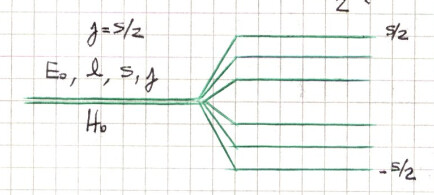
\includegraphics[width=0.5\textwidth]{images/fig_ft2_H_proy.jpg}


% \bibliographystyle{CBFT-apa-good}	% (uses file "apa-good.bst")
% \bibliography{CBFT.Referencias} % La base de datos bibliográfica

\end{document}

	
		\documentclass[10pt,oneside]{CBFT_book}
	% Algunos paquetes
	\usepackage{amssymb}
	\usepackage{amsmath}
	\usepackage{graphicx}
% 	\usepackage{libertine}
% 	\usepackage[bold-style=TeX]{unicode-math}
	\usepackage{lipsum}

	\usepackage{natbib}
	\setcitestyle{square}

	\usepackage{polyglossia}
	\setdefaultlanguage{spanish}
	



	\usepackage{CBFT.estilo} % Cargo la hoja de estilo

	% Tipografías
	% \setromanfont[Mapping=tex-text]{Linux Libertine O}
	% \setsansfont[Mapping=tex-text]{DejaVu Sans}
	% \setmonofont[Mapping=tex-text]{DejaVu Sans Mono}

	%===================================================================
	%	DOCUMENTO PROPIAMENTE DICHO
	%===================================================================

\begin{document}


% =================================================================================================
\chapter{Simetrías en mecánica cuántica}
% =================================================================================================

Las simetrías son las que originan las fuerzas, en algún sentido. Desde el punto de vista actual las
fuerzas (interacciones) tienen su origen en simetrías básicas que cumplen los constituyentes de la
materia.
Esta caracteerística de las simetrías es amén del hecho de su utilidad para resolver problemas.

En mecánica clásica tenemos el teorema de Noether 
\[
	\dpar{\Lag}{q_i} = 0 \quad \to \quad \dtot{}{t}\left( \dpar{\Lag}{\dot{q}_i} \right) = 
	\dtot{}{t}\left( p_i \right) = 0 \quad \rightarrow \quad \partial p_i = cte.
\]
Y $\Ham, \Lag$ no cambian con la transformación $q_i \longrightarrow q_i + \delta q_i$
\[
	\dpar{\Ham}{q_i} = 0 \quad \to \quad  
	\dtot{}{t}\left( p_i \right) = 0 \quad \rightarrow \quad \partial p_i = cte. 
\]

En mecánica cuántica definiremos un operador unitario $\$$ asociado a traslación/rotación. 
Pensemos en una transformación infinitesimal dada por $\$$
\[
	\mathbb{\$} = \mathbb{1} - i\frac{\varepsilon}{\hbar}G \qquad G \equiv \text{generador hermítico (de 
la transf.)}
\]

Sea el H invariante frente a $\$$, entonces 
\[
	S^\dagger HS = H \quad  \rightarrow \quad [H,\$] = 0 
\]
Luego,
\[	
	[H,G]=0 \rightarrow \dtot{G}{t} = 0 \rightarrow G \;\text{es cte. de movimiento}
\]
es decir que el generador de la transformación es una constante.
Esto significa que el autovalor asociado no varía con el tiempo. Es algún {\it deja vu} del teorema
de Noether de la mecánica clásica.

Sea $H\Ket{n} = E_n \Ket{n}$, luego como $[H,G]=0$ se tiene 
\[
	G\Ket{n} = k\Ket{n} \qquad \text{pués} \qquad H(G\Ket{n}) = E_n(k\Ket{n})
\]
de modo que tienen la misma base de autoestados. Si no hay degeneración
\[
	G\ket{n} = k(\text{fase}) \Ket{n}
\]
mientras que si hay degeneración $G\Ket{n}\neq \Ket{n}$.
Invariancia frente a traslaciones $G=\vb{p}$ e invariancia frente a rotaciones $G=\vb{J}$ [?].
Acá tal vez quise poner invariancia frente a traslaciones, $\vb p$ constante y frente a rotaciones
$\vb J$ constante.

Hay degeneraciones, por ejemplo con $[H,J^2]=0$ entonces $[H,J_z]$ lleva a degeneración $2j+1$
para $\Ket{n,\ell,m}$.

\subsection{Transformaciones discretas}

Durante algún tiempo se consideraron solo tres transformaciones discretas; P(paridad), C(carga) y
T(inversión temporal).
Toda interacción debería verificar estas tres simetrías. Se vio en los 50's que la fuerza débil
no cumple, en forma separada, CPT pero que las maneras de no cumplirla es tal que se conserva
CPT como un todo (siempre se deja de cumplir de igual manera).

{\bf  Simetría de paridad}

Es la reflexión especular.
Transforma un RHS en LHS. Es decir que hace 
\[
	\vb{x} \longrightarrow - \vb{x}
\]
con una matriz asociada
\[
	R = \begin{pmatrix}
	 -1 & 0 & 0 \\
	 0 & -1 & 0 \\
	 0 & 0 & -1
	\end{pmatrix}
\]

En mecánica cuántica solicitaremos un operador unitario llamado paridad que verifique 
\[
	\Ket{\alpha} \longrightarrow \Pi\Ket{\alpha} = \Ket{\alpha'}
\]
si $\Pi$ es unitario y $\Pi^1=\mathbb{1}$ entonces es hermítico.
\begin{figure}[htb]
	\begin{center}
	\includegraphics[width=0.6\textwidth]{images/teo2_16.pdf}
	\end{center}
	\caption{}
\end{figure} 
Queremos que refleje el $\Braket{\hat{x}}$ 
\[
	\Braket{\alpha'|\vb{x}|\alpha'} = - \Braket{\alpha|\vb{x}|\alpha} 
\]
\[
	\Braket{\alpha|\Pi^\dagger\vb{x}\Pi|\alpha} = - \Braket{\alpha|\vb{x}|\alpha} \rightarrow
	\Pi^\dagger\vb{x}\Pi = -\vb{x} 
\]
y entonces 
\[
	\{\vb{x},\Pi\} = 0,
\]
anticonmuta con \vb{x}. Debido a ello 
\[
	\Pi\Ket{\vb{x}'} = \Ket{-\vb{x}'} \qquad \Pi^2 \equiv \mathbb{1}
\]
lo cual dice que los autovalores son $\pm 1$ y $\Pi$ es unitario y hermítico.
Como $\hat{\Pi}$ no depende del tiempo (lo aplico a $\vb P$)
\notamargen{No veo el vínculo de que no variando con el tiempo se aplique a \vb{p}.}
\[
	\Pi^\dagger\vb{p}\Pi = \Pi^\dagger\dtot{\vb{x}}{t}\Pi = \dtot{}{t}(\Pi^\dagger\vb{p}\Pi) = 
	\dtot{-\vb{x}}{t} \rightarrow \{\vb{p},\Pi\}= 0
\]
y vemos que anticonmuta con \vb{p}.
Se ve que \vb{x}, \vb{p} son operadores impares. 

En cambio, el pseudovector $\vb{L}=\vb{x}\times\vb{p}$ es un operador par, entonces 
\[
	[\vb{L},\Pi] = 0 \qquad [\vb{J},\Pi] = 0
\]
\begin{figure}[htb]
	\begin{center}
	\includegraphics[width=0.6\textwidth]{images/teo2_17.pdf}
	\end{center}
	\caption{}
\end{figure} 
Que conmuta con \vb{J} puede verse de pedirle que 
\[
	[\Pi,\mathcal{D}(R)] = 0 \longrightarrow [\Pi,\vb{J}] = 0 ,
\]
donde $\mathcal{D}(R) = \exp(- i \vb J \cdot \nver \phi / \hbar)$, puesto que esta cosa vale en 
mecánica clásica, donde se tenía
\[
	R^{\text{(paridad)}}R^{\text{(rotación)}} = R^{\text{(rotación)}} R^{\text{(paridad)}},
\]
y por ello se le pide que lo mismo valga en mecánica cuántica.
Esto nos dice que $\vb J$ es un operador par (un pseudovector).

Veamos cómo actúa sobre vectores y sobre escalares (productos internos),
\[
	\Pi^\dagger \Box \Pi =  \begin{cases} +{\Box} \quad \text{par}\quad\text{vector axial( 
	pseudovector)}\\  -\Box \quad \text{impar} \quad \text{vector polar} \end{cases}
\]
\[
	\Pi^\dagger \Box \Pi =  \begin{cases} +\Box \quad \text{par}\quad\text{escalar}\\
	-\Box \quad \text{impar} \quad \text{pseudoescalar} \end{cases}
\]

Así, por ejemplo, para $\vb{S}\cdot\vb{x}$ pseudoescalar se tiene
\[
	\Pi^\dagger \vb{S}\cdot\vb{x} \Pi = \Pi^\dagger \vb{S}\Pi \cdot\Pi^\dagger\vb{x} \Pi =
	\vb{S}\cdot(-\vb{x}) = -\vb{S}\cdot\vb{x}.
\]

Veamos ahora qué sucede con la función de onda bajo paridad.
\[
	\Psi_\alpha(x') = \Braket{x'|\alpha} = \Braket{x'|\Pi|\alpha} = \Braket{x'|\alpha'} = 
	\Braket{-x'|\alpha}
\]
y entonces la función de onda de un estado al que se le aplicó paridad será 
\[
	\Psi_{\alpha'}(x') = \Psi_\alpha(-x').
\]

Sea $\Ket{\alpha}$ autoestado de paridad, entonces considerando que $ [ H, \Pi] = 0 $ y no hay
degeneración (como en el caso del oscilador armónico),
\[
	\Pi\Ket{\alpha} = \pm \Ket{\alpha}
\]
los autovalores serán $\pm 1$
\[
	\Braket{x'|\alpha'} = \pm \Braket{x'|\alpha} = \Braket{-x'|\alpha} 
\]
\[
	\Psi_\alpha(-x') = \begin{cases} +\Psi_\alpha(x') \quad \text{función de onda par}\\ 
	-\Psi_\alpha(x') \quad \text{función de onda impar}\\ 
	\end{cases}
\]
no toda función de onda tiene paridad bien definida.
No hay que confundir la paridad de la función de onda con la del operador.
Un hamiltoniano que se conmute con $\Pi$ tendrá una descomposición en una parte par y en una impar.

Consideremos ahora problemas con simetrías radial, y queremos ver qué hace el operador paridad allí.
El cambio de paridad 
\[
	\vb{x} \to -\vb{x} 
\]
involucra
\[
	\left( r\to r, \theta \to \pi-\theta, \phi \to \phi+\pi \right).
\]
Entonces para
\[
	\Braket{x'|\alpha,\ell,m} = R_\alpha(r) Y_\ell^m(\theta,\phi), 
\]
con el cambio $ \vb{x} \; \to -\vb{x} $ será
\[
	Y_\ell^m(\pi-\theta,\phi+\pi) = (-1)^\ell Y_\ell^m(\theta,\phi)
\]
entonces
\[
	\Pi\Ket{\alpha,\ell,m} =  (-1)^\ell \Ket{\alpha,\ell,m}
\]
donde $\ell$ define la paridad y $(-1)^\ell$ es el autovalor de paridad.
Si $[H,\Pi] = 0$ y no hay degeneración
\[
	H \Ket{\a} = E_{\a} \Ket{\a} \qquad \qquad \Pi \Ket{\a} = \pm \Ket{\a}
\]

Para la partícula libre es $H = p^2/(2m)$ y $[H,\Pi] = 0$ pero lo feo es que siendo $\Ket{\vb p'}$ autoestado
de $H$, no es autoestado de $\Pi$,
\[
	\Pi \Ket{\vb p'} = \Ket{-\vb p'}.
\]
Esto surge por la degeneración de que $\Ket{\vb p'}, \Ket{-\vb p'}$ tienen la misma energía.
Luego, tengo que utilizar la {\it manganeta} habitual
\[
	\Ket{S} = \frac{1}{\sqrt{2}} \left( \: \Ket{\vb p'} + \Ket{-\vb p'} \: \right)
\]
y
\[
	\Ket{A} = \frac{1}{\sqrt{2}} \left( \: \Ket{\vb p'} - \Ket{-\vb p'} \: \right)
\]
que verifican
\[
	\Pi \Ket{S} = +1 \Ket{S} \qquad \qquad \Pi \Ket{A} = -1 \Ket{A}.
\]

Como $[\vb{L},\hat{\Pi}]=0$ un autoestado de \vb{L} es autoestado de $\hat{\Pi}$ .

\begin{ejemplo}{\bf De paridad}

Sean $\Ket{\a}, \Ket{\b}$ autoestados cumpliendo que
\[
	\Pi \Ket{\a} = \varepsilon_\a \Ket{\a} \qquad \qquad 
	\Pi \Ket{\b} = \varepsilon_\b \Ket{\b}
\]
donde $\varepsilon_{\a,\b} = \pm 1$
Luego $ \Braket{\a|\vb X|\b} = 0 $ si $\varepsilon_\a = \varepsilon_\a$
\[
	\Braket{ \b | \pi^2 \vb X \pi^2 | \a } = - \varepsilon_\a \varepsilon_\b 
	\Braket{ \b | \vb X | \a } = \Braket{ \b | \vb X | \a}
\]
entonces se tienen que 
\[
	\begin{cases}
		\varepsilon_\a = - \varepsilon_\b \qquad \text{ el elemento no será nulo.} \\
		\varepsilon_\a \neq - \varepsilon_\b \qquad \text{ el elemento es nulo.}
	\end{cases}
\]
Entonces
\[
	\Braket{\a|\vb X|\a} = 0.
\]
La utilidad de esto es que dada la paridad podemos descartar probabilidades. 
Dos cosas pares no pueden interactuar con una impar y así.
 
\end{ejemplo}


\subsection{Teorema}

Sea $[H,\pi]=0$ y $\Ket{n}$ autoestados no degenerados de $H$ 

	$\Rightarrow$ $\Ket{n}$ es autoestado de $\Pi$.

La demostración 
\[
	\left(\frac{1}{2}\pm \frac{\Pi}{2}\right)\Ket{n} = \frac{\Pi^2\pm\Pi}{2}\Ket{n} = 
	\Pi \left( \frac{\pm 1+\Pi}{2}\right)\Ket{n} = \pm\Pi \frac{1\pm\Pi}{2}\Ket{n}
\]
y entonces es autoestado de paridad con autovalor $\pm 1$. 
\[
	H\frac{1}{2}\left(1\pm\Pi\right)\Ket{n} = \frac{1}{2}E_n\Ket{n} \pm \frac{E_n}{2}\Pi\Ket{n} =
	E_n\left[ \left( \frac{1}{2} \pm \frac{\Pi}{2}\right) \right]
\]
y es autoestado de $H$, de manera que 
\[
	\left( \frac{1\pm\Pi}{2}\right)\Ket{n} = \Ket{n} \Rightarrow \Ket{n} \quad \text{es autoestado de 
paridad}
\]
\[
	\frac{1}{2}\Ket{n} \pm \frac{\Pi}{2}\Ket{n} = \Ket{n}
\]
\[
	\pm \frac{\Pi}{2}\Ket{n} = +\frac{\Ket{n}}{2} \Rightarrow \Pi\Ket{n} = \pm\Ket{n}
\]
Un caso donde falla el teorema 
\[
	[H,\Pi]=0 \quad \text{con} \quad H=\frac{p^2}{2m} 
\]
pero $\Ket{p'}$ no es autoestado de $\Pi$ por la degeneración $\Ket{p'},\Ket{-p'}$ son ambos correspondientes 
al autovalor $p'2/2m$
\[
	\frac{\hat{p}^2}{2m}\Ket{p'} = \frac{{p'}^2}{2m}\Ket{p'} \qquad  \qquad 
	\frac{\hat{p}^2}{2m}\Ket{-p'} = \frac{{p'}^2}{2m}\Ket{-p'}
\]
\[
	\Pi\Ket{p'}= \Ket{-p'}
\]
y $\Ket{p'}$ no es autoestado de $\Pi$.

Para un oscilador armónico será
\[
	H = \frac{p^2}{2m} - \frac{m \omega^2 x^2}{2}, \qquad [H,\Pi] = 0
\]
y los estados tienen paridad definida, no son degenerados. Luego, $\Ket{n}$ tendrán paridad $(-1)^n$.

\subsection{Reglas de selección de paridad $\Pi$}

Sean $\Ket{\alpha}, \Ket{\beta}$ autoestados de paridad 
\[
	\Pi\Ket{\alpha} = \varepsilon_\alpha \Ket{\alpha} \qquad\qquad
	\Pi\Ket{\beta} = \varepsilon_\beta \Ket{\beta}
\]
siendo para el caso impar
\[
	\Braket{\beta|\Box|\alpha} = - \Braket{\beta|\Pi^\dagger\Box\Pi|\alpha} =
	-\varepsilon_\alpha \varepsilon_\beta \Braket{\beta|\Box|\alpha},
\]
y en el caso par
\[
	\Braket{\beta|\Box|\alpha} = \Braket{\beta|\Pi^\dagger\Box\Pi|\alpha} =
	\varepsilon_\alpha \varepsilon_\beta \Braket{\beta|\Box|\alpha}
\]

Si el operador $\Box$ es impar (como $\vb{x}, \vb{p}$) entonces $\varepsilon_\alpha=1,
\varepsilon_\beta=-1$ o bien $\varepsilon_\alpha=-1,\varepsilon_\beta=1$.

Si el operador $\Box$ es par (como $\vb{L}, \vb{S}$) entonces $\varepsilon_\alpha=1,
\varepsilon_\beta=1$ o bien $\varepsilon_\alpha=-1,\varepsilon_\beta=-1$.

\begin{itemize}
 \item Operadores impares solo conectan estados de paridad opuesta.
 \item Operadores pares solo conectan estados de la misma paridad.
\end{itemize}

Partiendo desde 
\[
	\Braket{\beta|\vb{x}|\alpha} = 0, 
\]
entonces tenemos
\[
	\int\int dx'dx''\Braket{\beta|x''}\Braket{x''|\vb{x}|x'}\Braket{x'|\alpha}= 0
\]
y como es $\Braket{x''|\vb{x}|x'} = x' \delta(x' -x'')$
\[
	\int_{-\infty}^{+\infty} dx'\Braket{\beta|x'} x' \Braket{x'|\alpha} =
	\int_{-\infty}^{+\infty} dx'\Psi_\beta^*(x') x' \Psi_\alpha (x')
\]

\begin{ejemplo}{\bf Ejercicio 2}
 
Sea $\Tau_{\vb j}$ traslación y $\mathcal{D}(\nver,\phi)$. Habría que probar, parece que
\[
	a) \; [ \Tau_{\vb j}, \Tau_{\vb j'}] = 0
\]
\[
	b) \; [ \mathcal{D}(\nver',\phi), \mathcal{D}(\nver,\phi) ] \neq 0
\]
\[
	c) \; [\Tau_{\vb j}, \Pi] \neq 0
\]
\[
	d) \; [\mathcal{D}(\nver,\phi), \Pi] = 0
\]
Esto podría hacerse empleando background de anteriores capítulos.
 
\end{ejemplo}

\begin{ejemplo}{\bf Ejercicio 4}
 
Se tiene
\[
	Y_\ell^{j=\ell \pm 1/2,m} = \frac{1}{\sqrt{2\ell+1}} 
	\begin{pmatrix}
		\pm \sqrt{\ell \pm m + 1/2 } & Y_\ell^{m-1/2}(\theta,\varphi) \\
		\\
		\pm \sqrt{\ell \mp m + 1/2 } & Y_\ell^{m+1/2}(\theta,\varphi)
	\end{pmatrix}
\]
El problema es una combinación de s=1/2 sumado a un potencial esféricamente simétrico; es
decir espacios del tipo $\Braket{\theta,\varphi|\ell,m} \otimes \Ket{\text{spin}}$.
Los estados de spin son los de siempre $\Ket{+}, \Ket{-}$ y se tiene $\vb J = \vb L + \vb S$
con $|\ell-s| \leq j \leq |\ell+s|$.

La parte a) es sencillamente
\[
	Y_{\ell=0}^{j=1/2,m=1/2} = \begin{pmatrix}
	                        Y_0^0\\
	                        \\
	                        0
	                       \end{pmatrix} = \frac{1}{\sqrt{4\pi}}
	                       \begin{pmatrix}
	                        1 \\
	                        \\
	                        0
	                       \end{pmatrix}
\]

La parte b) involucra obtener $( \pe{\sigma}{x} ) Y_{\ell=0}^{j=1/2,m=1/2}$ en términos
de $Y_\ell^{j,m}$.
El producto escalar de $\vb \sigma$ se pone en función de armónicos esféricos, lo cual será
\[
	\pe{\sigma}{x} = r ( \sin\theta\cos\vp \:\sigma_x + \sin\theta\sin\vp \:\sigma_y +
	\cos\vp \:\sigma_z )
\]
y entonces
\[
	\pe{\sigma}{x} \: Y_{\ell=0}^{j=1/2,m=1/2} =
	\frac{r}{\sqrt{4\pi}}
	\left( 
	\begin{bmatrix}
	 0 \\
	 \cos\theta\sin\vp
	\end{bmatrix} +
	\begin{bmatrix}
	 0 \\
	 i\sin\theta\sin\vp
	\end{bmatrix} +
	\begin{bmatrix}
	 \cos\vp \\
	 0
	\end{bmatrix}
	\right)
\]
lo cual se puede, usando la tablita de armónicos esféricos, llevar a la forma
\[
	\frac{r}{\sqrt{4\pi}} 
	\begin{pmatrix}
	 \cos\theta \\
	 \sin\theta\euler^{i\vp}
	\end{pmatrix} =
	\frac{r}{\sqrt{4\pi}} 
	\begin{pmatrix}
	 Y_1^0(\vp,\theta) \sqrt{4\pi/3} \\
	 Y_1^1(\vp,\theta) \sqrt{8\pi/3}
	\end{pmatrix} =
	- r Y_{\ell=1}^{j=1/2,m=1/2}.
\]

La parte c) empezamos con $\ell=0$ finalizando con $\ell=1$. El $\pe{s}{x} = \hbar  \pe{\sigma}{x}$ 
no varía ante rotaciones por ser un escalar. 
Entonces por qué varió $\ell$, la resppuesta es porque $\pe{s}{x}$ es un pseudoescalar y la transformación
es de paridad. La paridad del estado final es impar.

 
\end{ejemplo}



\section{Inversión temporal (reversión de movimiento)}

Es simplemente el reemplazo
\[
	t \longrightarrow -t
\]
que en mecánica clásica sería como {\it pasar la película hacia atrás}. Los sistemas que verifican
esta simetrías son aquellos para los cuales no es distinguible la evolución hacia atrás o hacia adelante.
En mecánica clásica los sistemas no disipativos cumplen estas condiciones; en lo referente a ir y volver
partiendo y terminando en un mismo punto con iguales condiciones.

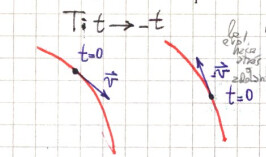
\includegraphics[width=0.4\textwidth]{images/fig_ft2_temporal_1.jpg}

Esto surge del carácter de las ecuaciones de Newton. 
En sistemas sin fuerzas disipativas se tiene 
\[
	m \ddot{x} = - \dtot{}{x} V(x)
\]
siendo $x(t)$ y $x(-t)$ soluciones de $\vb{F} = m\vb{a}$ puesto que si $t\to-t$ se tiene
\[
	m \ddot{x} = - \dtot{}{x} V(x)
\]
dado que 
\[
	\dtot[2]{x(t)}{t} = \dtot[2]{x(-t)}{t}.
\]
En un sistema disipativo existe una pérdida de energía en ir y venir por lo cual no acabamos en la
misma situación.

En mecánica cuántica tendremos 
\[
	i \hbar \dpar{\Psi(x,t)}{t} = \left( -\frac{\hbar^2\nabla^2}{2m} + V \right)\Psi(x,t)
\]
y si hacemos el cambio $t\to -t$
\[
	i \hbar \dpar{\Psi(x,-t)}{t} = -i \hbar \dpar{\Psi(x,t)}{t}  = 
	- \left( -\frac{\hbar^2\nabla^2}{2m} + V \right)\Psi(x,t)
\]
se ve que $\Psi(x,-t)$ no es solución de Schrödinger. La ecuación de Schrödinger no se queda
inamovible ante tal cambio.

Pero notemos que $\Psi^*(x,-t)$ sí cumple la ecuación de Schrödinger
\[
	i \hbar \dpar{\Psi^*(x,-t)}{t} = -i \hbar \dpar{\Psi^*(x,t)}{t} 
\]

Entonces necesitamos un operador que respete esta característica.
Necesitaré el producto interno conjugado 
\[
	\Psi_\alpha(x') = \Braket{x'|\alpha} \qquad
	\Psi^*_\alpha(x') = \Braket{x'|\alpha}^* = \Braket{\alpha|x'}.
\]
Se necesitará un operador $\hat{\Theta}$, y veremos que no puede ser unitario.
Dados dos estados
\[
	\Ket{\tilde{\alpha}} = \hat{\Theta}\Ket{\alpha} \qquad 
	\Ket{\tilde{\beta}} = \hat{\Theta}\Ket{\beta},
\]
si el operador era unitario se tenía que se conservaba el producto interno 
\[
	\Braket{\hat{\beta}|\hat{\alpha}} = 
	\Braket{\beta|\hat{\Theta}^\dagger\hat{\Theta}|\alpha} =
	\Braket{\beta|\mathbb{1}|\alpha} = \Braket{\beta|\alpha}
\]
y no obtengo un producto interno conjugado.

Pediremos antiunitariedad y antilinealidad al operador $\hat{\Theta}$, es decir
\begin{itemize}
 \item Antiunitariedad 
 \[
	\Braket{\hat{\beta}|\hat{\alpha}} = \Braket{{\beta}|{\alpha}}^*
\]
 \item Antilinealidad
\[
	\hat{\Theta}[ C_\alpha\Ket{\alpha} + C_\beta\Ket{\beta}] = 
	C_\alpha^*\hat{\Theta}\Ket{\alpha} + C_\beta^*\hat{\Theta}\Ket{\beta}
\]
\end{itemize}

Todo operador antiunitario y antilineal puede escribirse como producto 
\[
	\Theta = U K
\]
donde $U$ es unitario y $K$ la conjugación compleja, que opera
\[
	K c \Ket{\a} = c^* K \Ket{\a}.
\]
Queremos ver qué hace $K$ y para ello consideramos un $\Ket{\a}$ tal que
\[
	\Ket{\a} = \sum_{a'} \Ket{a'} \Braket{ a' | \a } \qquad 
	K \Ket{\a} = \sum_{a'}  \Braket{ a' | \a }^* K\Ket{a'}
\]
donde vemos que en el segundo término no hace nada; $K$ sobre un autoket no cambia nada, pués
$\Ket{\a}$ es un autoestado en la base canónica. La expresión del operador $K$ dependerá de la
base sobre la cual trabaje.

Para ver que un operador es antiunitario simplemente deberíamos chequear si cumple las propiedades
1 y 2. Así
\[
	UK ( c_\a \Ket{\a} + c_\b \Ket{\b} ) = 
	c_\a^* U K \Ket{\a} + c_\b^* U K \Ket{\b}
\]
y vemos que $UK$ es antilineal.

\notamargen{Los operadores antiunitarios actúan de forma misteriosa sobre un bra.}

\begin{ejemplo}{\bf Descolgado}
$K$ no cambia los autoestados, porque en base canónica 
un autoestado tiene un solo elemento (1) que no es nulo.
\begin{multline*}
	K(C\Ket{\alpha}) = CK\Ket{\alpha} = C^*K(\sum_{a'} \Ket{a'}\Braket{a'|\alpha}) = \\
	C^* (\sum_{a'} \Braket{a'|\alpha}^* K \Ket{a'}) =
	C^* (\sum_{a'} \Braket{a'|\alpha}^* \Ket{a'})  
\end{multline*}

\end{ejemplo}

Veamos que $UK$ es antiunitario. Tenemos dos estados 
\[
	\Ket{\hat{\alpha}} = UK \Ket{\alpha} = \sum_{a'} \Braket{a'|\alpha}^* U\Ket{a'} \qquad 
	\Ket{\hat{\beta}} = UK \Ket{\beta} = \sum_{a''} \Braket{a''|\beta}^* U\Ket{a''},
\]
y sobre este último tomo dual conjugado, lo cual puede verse como un {\it trick} para no reverla 
cómo opera $K$ sobre un bra,
\[
	\Bra{\hat{\beta}} = \sum_{a''} \Braket{a''|\beta} \Bra{a''}U^\dagger
\]
entonces, desarrollando
\[
	\Braket{\hat{\beta}|\hat{\alpha}} = \sum_{a''} \Braket{a''|\beta} \Bra{a''}U^\dagger
	\sum_{a'} \Braket{a'|\alpha}^* U\Ket{a'},
\]
se tiene
\begin{multline*}
	\sum_{a',a''} \Braket{a''|\beta} \Braket{a'|\alpha}^* \Bra{a''}U^\dagger U\Ket{a'} =
	\sum_{a'} \Braket{a'|\beta} \Braket{a'|\alpha}^* = \\
	\sum_{a'} \Braket{\beta|a'}^* \Braket{a'|\alpha}^* = \Braket{\beta|\alpha}^*
\end{multline*}
y entonces UK es antinunitario.

Notemos que no se define $\hat{\Theta}^\dagger$ actuando sobre bras. La demostración anterior esperó a 
quitarse de encima $\hat{K}$ para hacer dual conjugado al $\Ket{\tilde{\beta}}$.

\subsection{Operadores ante $\hat{\Theta}$}

Usaremos la notación 
\[
	\Ket{\tilde{\alpha}} = \hat{\Theta} \Ket{\alpha}
\]
donde $\Ket{\tilde{\alpha}}$ es el estado reversión temproal. Es de esperar que si $\Pi \Ket{\vb x} = 
\Ket{-\vb x}$ entonces $ \Theta \Ket{\vb p} = \Ket{-\vb p}$, pero veremos lo que sucede en los valores
de expectación.
hay que tener en cuenta 
\[
	\Theta^\dagger \Theta = \mathbb{1}
\]
pues $\Theta^\dagger$ no está definido.

Entonces, viendo valores de expectación, sería razonable esperar que 
\[
	\Braket{\hat{\alpha}|\vb{p}|\hat{\alpha}} = - \Braket{{\alpha}|\vb{p}|{\alpha}}\qquad 
	\Braket{\hat{\alpha}|\vb{x}|\hat{\alpha}} = \Braket{{\alpha}|\vb{x}|{\alpha}}\qquad 
\]
Veamos qué sucede para operadores hermíticos como $\hat{\mathbb{O}}$. Siendo
\[
	\Braket{\alpha|\mathbb{O}|\alpha} = \Braket{\alpha|\gamma}
\]
\[
	\Braket{\hat{\alpha}|\hat{\gamma}}^* = \Braket{\alpha|\gamma} \Rightarrow 
	\Braket{\hat{\alpha}|\hat{\gamma}} = \Braket{\gamma|\alpha}
\]
y como $\Braket{\hat{\alpha}|\Theta|\gamma} = \Braket{\hat{\alpha}|\Theta\mathbb{O}|\alpha}$.
Luego metemos un $\Theta^{-1}\Theta = 1$
\[
	\Braket{\hat{\alpha}|\Theta\mathbb{O}\Theta^{-1}\Theta|\alpha} =
	\Braket{\hat{\alpha}|\Theta\mathbb{O}\Theta^{-1}|\hat{\alpha}} = \Braket{\alpha|\mathbb{O}|\alpha}
\]

Notamos que no se aplica $\Theta$ sobre bra alguno y tenemos $\Theta$ no unitario. 
\notamargen{Chequear que esto esté claro, porque en la carpeta tengo otra versión de esta cuenta.}

Entonces requeriremos 
\[
	\Theta \hat{p} \Theta^{-1} = -\hat{p} \qquad \Theta \hat{j} \Theta^{-1} = -\hat{j}
\]
\[
	\hat{\Theta}\hat{p} = -\hat{p}\hat{\Theta} \quad \Rightarrow 
	\quad \{ \hat{\Theta},\hat{p}\} = 0
\]
como para $\vb{p},\vb{J}$ operadores impares 
\[
	\Theta \hat{x} \Theta^{-1} = \hat{x}
\]
\[
	\hat{\Theta}\hat{x} = -\hat{x}\hat{\Theta} \quad \Rightarrow 
	\quad [ \hat{\Theta},\hat{x} ] = 0
\]
y $\vb{x}$ operador par.

Los operadores pares conmutan con $\Theta$,
\[
	\Theta \Ket{\vb{x}'} =  \Ket{\vb{x}'} \qquad \qquad
	\Theta \Ket{\vb{p}'} =  \Ket{-\vb{p}'} ,
\]
y entonces tendrán base en común.


\begin{figure}[htb]
	\begin{center}
	\includegraphics[width=0.6\textwidth]{images/teo2_18.pdf}
	\end{center}
	\caption{}
\end{figure} 

Cualquier hamiltoniano razonable
\[
	H = \frac{p^2}{2m} + V(\vb x)
\]
es par y conmutará con $\Theta$. Consideramos que $ V(\vb x)$ se puede poner en serie de potencias
respecto de $\vb x$ y asimismo $ [ H, \Theta ] = 0 $.
Veamos ahora la continuidad para $\Ket{\a} = \int d^3x' \Ket{x'}\Braket{x'|\a}$ que se convierte en
\[
	\Theta \Ket{\a} = \int d^3x' \Braket{x'|\a}^*  \Theta\Ket{x'} = 
	\int d^3x' \Ket{x'} \Braket{x'|\a}^* 
\]
donde el braket último dentro de la integral es $\psi^*_{\a}(x')$.



Pero físicamente, ¿qué significa que $H, \Theta$ conmuten? Veamos el hamiltoniano ante reversión de 
movimiento, considerando para ello la reversión de un sistema en estado $\Ket{\alpha}$, si su evolución
un $\delta t$ está dada por
\[
	\Ket{\alpha, t=\delta t} = \left( \mathbb{1} - i\frac{\delta t}{\hbar} H \right) \Ket{\alpha}
\]
Si el hamiltoniano es invariante ante reversión temporal debería ser lo mismo 
\[
	\underbrace{U \Theta}_{+\delta t} \Ket{\alpha} = \underbrace{\Theta U}_{-\delta t} \Ket{\alpha},
\]
es decir que estamos pidiendo que se obtenga el mismo estado.

\begin{itemize}
 \item Si revertimos el movimiento y evolucionamos $\delta t$.
 \item Si evolucionamos hacia atrás $-\delta t$ y revertimos el movimiento.
\end{itemize}
\begin{figure}[htb]
% 	\begin{center}
	\includegraphics[width=0.6\textwidth]{images/teo2_19.pdf}
	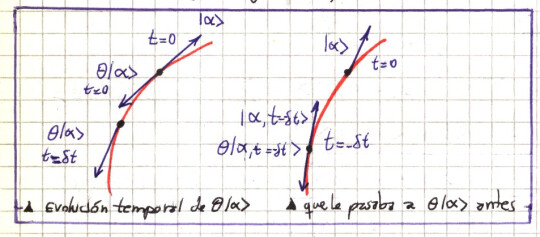
\includegraphics[width=0.6\textwidth]{images/fig_ft2_temporal_2.jpg}
% 	\end{center}
	\caption{}
\end{figure} 
Veamos que vale lo anterior, pensando que si vale se tiene 
\[
	\left( 1- i\frac{\delta t}{\hbar} H\right) \Theta \Ket{\alpha} =
	\Theta \left( 1 + i\frac{\delta t}{\hbar} H \right) \Ket{\alpha}
\]
\[
	- i\frac{\delta t}{\hbar} H \Theta \Ket{\alpha} =  \Theta
	i\frac{\delta t}{\hbar} H \Ket{\alpha} 
\]
\[
	- i H\Theta \Ket{\alpha} = \Theta (i H \Ket{\alpha} )
\]
\[
	[H,\Theta] = 0
\]

Si $\Theta$ era unitario teníamos la relación de anticonmutación $\{ H, \Theta \}=0$ 
lo cual lleva a absurdos.
Si $\{ H,\Theta \} = 0$ tendríamos
\[
	\Theta^{-1} \frac{p^2}{2m} \Theta = - \frac{p^2}{2m} < 0
\]
partícula libre con energía negativa. Justificaría así energías negativas hasta el infinito
y pierde significado el concepto de ``piso'' del estado fundamental.
Por ello $H$ debe ser par frente a $\Theta$.

\subsection{Función de onda}

\notamargen{Esto es lo que antes metí como ``la continuidad''. Claramente hay que consolidar
las dos cosas.}
Sea en $t=0$ un sistema en el estado $\Ket{\alpha}$
\[
	\Ket{\alpha} = \int dx' \Braket{x'|\alpha} \Ket{x'} 
\]
\[
	\Theta\Ket{\alpha} = \int dx' \Braket{x'|\alpha}^* \Theta \Ket{x'} =
	\int dx' \Braket{x'|\alpha}^* \Ket{x'} 
\]
\[
	\Psi_\alpha (x') \longrightarrow \Theta \longrightarrow \Psi_\alpha^* (x')
\]
Esto era lo que {\it vimos} en la ecuación de Schrödinger.

\subsection{Reversión de movimiento sobre \vb{J}}

Veamos qué hace $\Theta$ sobre autoestados de momento angular. No se puede decir que
$\Theta \Ket{\vb{J}} = \Ket{-\vb J}$ puesto que carece de sentido al no conmutar $J_x,J_y,J_z$ entre ellos.
El $\vb J$ no tiene expresión en términos de numeritos $j_x, j_y, j_z$.
Analizaremos $\Ket{\ell,m}$
\[
	Y_\ell^m(\theta,\phi) \longrightarrow\Theta\longrightarrow Y_\ell^m(\theta,\phi)^* =
	Y_\ell^{-m}(\theta,\phi)(-1)^m
\]
\[
	\Theta \Ket{\ell,m} \equiv (-1)^m \Ket{\ell,-m}
\]

Lo que hace $\Theta$ es invertir la componente de $\hat{z}$ y alterar la fase. Se ve que 
\[
	\Theta^2 = \mathbb{1}
\]
con $j$ par.

\subsection{Reversión para sistemas de spin $1/2$}

\notamargen{Esto vale para los casos de spin entero, donde se trabaja con $Y_\ell^m$.}
Sea un estado general up de spin $\Ket{\hat{n};+}$, que se obtiene con dos rotaciones 
\[
	\hat{S}\cdot\hat{n} \Ket{\hat{n};+} = \frac{\hbar}{2} \Ket{\hat{n};+}
\]
entonces
\[
	\euler^{-i\frac{\alpha}{\hbar}S_z}\euler^{-i\frac{\beta}{\hbar}S_y} \Ket{+} \equiv
	 \Ket{\hat{n};+}
\]
\[
	\Theta \Ket{\hat{n};+} = \euler^{-i\frac{\alpha}{\hbar}S_z}\euler^{-i\frac{\beta}{\hbar}S_y} =
	\euler^{-i\frac{\alpha}{\hbar}S_z}\euler^{-i\frac{\beta}{\hbar}S_y} \eta\Ket{-}
\]
\[
	\Theta \Ket{\hat{n};+} = \eta \Ket{\hat{n};-}
\]
pero 
\[
	\Ket{\hat{n};-} = \euler^{-i\frac{\alpha}{\hbar}S_z}\euler^{-i\frac{\beta}{\hbar}S_y}\Ket{+}
\]
dado que 
\[
	 \euler^{-i\frac{\pi}{\hbar}S_y} \Ket{+} = \Ket{-}
\]
\[
	\Theta \Ket{\hat{n};+} = \eta \euler^{-i\frac{\alpha}{\hbar}S_z}\euler^{-i\frac{\beta}{\hbar}S_y}
	\euler^{-i\frac{\pi}{\hbar}S_y} \Ket{+}
\]
\[
	\Theta = \eta \euler^{-i\frac{\pi}{\hbar}S_y} \text{(Para sistemas de spin 1/2)}
\]
donde 
\[
	\Theta\Ket{+} = \eta_+ \Ket{-} \qquad \Theta\Ket{-} = \eta_- (-\Ket{+})
\]
y como
\[
	\Theta^2 = -\mathbb{1}
\]
\begin{multline*}
	\Theta^2 ( c_+\Ket{+} + c_-\Ket{-}) = \Theta ( c_+^*\eta_+\Ket{-} + c_-^*\eta_-\Ket{+}) = \\
	-c_+\eta^*\eta \Ket{+} - c_-\eta^*\eta \Ket{-} = -( c_+\Ket{+} + c_-\Ket{-}) 
\end{multline*}
luego
\[
	\Theta\Ket{j,m} = i^{2m} \Ket{j,-m} = (-1)^m \Ket{j,-m}
\]
para todo $j$ entero o semientero.

\begin{ejemplo}{\bf Para casos de spin 1/2}

Esto es muy parecido a lo anterior, pero copio acá porque difieren en cosas. Consolidar más adelante.
Se tienen
\[
	\Theta J = - J \Theta, \qquad \Theta\Ket{\pm}  = \eta_{\pm} K \Ket{\mp}
\]
donde $\eta$ es la fase y recordemos que $K$ no hace nada. 
Un estado genérico $\Ket{\a} = c_+ \Ket{+} + c_- \Ket{-}$ cumple
\[
	\begin{cases}
		\Ket{-} = \euler^{ - i \pi S_y / \hbar } K \Ket{+} \\
		\euler^{ - i \pi S_y / \hbar } \Ket{-} = - \Ket{+} \text{ Vuelta en $2\pi$ que altera el signo} 
	\end{cases}
\]
Combinando este sistemita llegamos a una expresión para $\Theta$
\[
	\Theta = \eta \euler^{ - i \pi S_y / \hbar } K,
\]
donde esto vale solo para casos de spin $1/2$. Entonces
\[
	\Theta\Ket{\a} = c_+^* \eta \Ket{+} + c_-^* \eta \Ket{-}
\]
y
\[
	\Theta^2 \Ket{\a} = -c_+ \Ket{+} - c_- \Ket{-}
\]
o bien $\Theta^2 = - \mathbb{1}$. Se puede escribir entonces
\[
	\Theta\Ket{j,m} = i^{2m} \Ket{j,-m} .
\]
\end{ejemplo}


\subsection{Teorema}

Sea $H$ invariante ante $\Theta$ y los $\Ket{n}$ no degenerados, entonces la autofunción de energía puede 
hacerse real tomando una fase apropiada.
Recordemos que $[H,\Theta]=0$.

Demostración 
\[
	H\Theta\Ket{n} = \Theta H \Ket{n} = E_n \Theta \Ket{n} \longrightarrow \Theta \Ket{n} = \delta\Ket{n}
\]
donde la fase $\delta$ puede hacerse uno (luego se hará)
\[
	\Psi_n = \Braket{\vb{x}|n} \longrightarrow \Psi_{\tilde{n}} = \Braket{\vb{x}|\tilde{n}} =
	\Braket{n|\vb{x}} = \Psi_n (\vb{x})^*
\]
y esto por ser antinunitario $\Theta$
\[
	\Psi_{\tilde{n}} = \Braket{\vb{x}|\Theta|n} = \delta\Braket{\vb{x}|n} = \delta\Psi_n(\vb{x})
\]
sea $\delta = 1 $ entonces 
\[
	\Psi_n^* = \Psi_n \quad \longrightarrow \quad \Psi_n(\vb{x}) \in \mathbb{R} 
\]
Esto vale cuando no hay degeneración; cuando la halla deja de valer y pueden aparecer componentes
imaginarias en la función de onda.

Si le aplico al sistema transformaciones dadas por operadores que conmutan con el H no lo sacamos del 
autoestado en que se encuentra con el paso del tiempo.
En ese sistema solo será razonable medir variables representadas por esos operadores; puesto que de lo 
contrario estamos alterando el sistema y nos es imposible saber donde ha quedado.

\begin{ejemplo}{\bf Fermiones}

Consideremos un sistema de $m$ fermiones cuyo estado se describe con $[H,\Theta]=0$. Entonces
$ H\Ket{n} = E_n \Ket{n}$ y $ H( \Theta \Ket{n} ) = E_n ( \Theta \Ket{n} ) $ donde suponemos que $\Theta\Ket{n}$
y $\Ket{n}$ representan el mismo estado físico y son iguales salvo una fase.
Es decir,
\[
	\Theta \Ket{n} = \euler^{i \delta} \Ket{n}
\]
luego
\[
	\Theta^2 \Ket{n} = \euler^{-i \delta} \Theta \Ket{n} = \Ket{n}.
\]
Si j es impar, número impar de fermiones, los estados $\Theta \Ket{n}$ y $\Ket{n}$ son estados distintos,
aunque con la misma energía. Hay degeneración.
Puedo romper esa degeneración aplicando un campo magnético $\vb B$. Allí surgirá que se puede ver, visualmente,
observada la diferencia entre ir hacia $t$ e ir hacia $-t$.
\notamargen{¿Qué se habrá querido decir con esto?}
 
\end{ejemplo}


% \bibliographystyle{CBFT-apa-good}	% (uses file "apa-good.bst")
% \bibliography{CBFT.Referencias} % La base de datos bibliográfica

\end{document}

	
		\documentclass[10pt,oneside]{CBFT_book}
	% Algunos paquetes
	\usepackage{amssymb}
	\usepackage{amsmath}
	\usepackage{graphicx}
% 	\usepackage{libertine}
% 	\usepackage[bold-style=TeX]{unicode-math}
	\usepackage{lipsum}

	\usepackage{natbib}
	\setcitestyle{square}

	\usepackage{polyglossia}
	\setdefaultlanguage{spanish}
	



	\usepackage{CBFT.estilo} % Cargo la hoja de estilo

	% Tipografías
	% \setromanfont[Mapping=tex-text]{Linux Libertine O}
	% \setsansfont[Mapping=tex-text]{DejaVu Sans}
	% \setmonofont[Mapping=tex-text]{DejaVu Sans Mono}

	%===================================================================
	%	DOCUMENTO PROPIAMENTE DICHO
	%===================================================================

\begin{document}

% =================================================================================================
\chapter{Métodos perturbativos}
% =================================================================================================

Se basan en un hamiltoniano
\[
	H = H_0 + \lambda V \qquad \lambda \ll 1, 
\]
donde $\lambda$ es un parámetro para controlar la perturbación y donde
\[
	H_0\Ket{n^{(0)}} = E_n^{(0)}\Ket{n^{(0)}}
\]
es el problema sin perturbar.
\notamargen{En la carpeta la notación es un poco diferente. Se dice que el espectro es discreto
y que no hay degeneración. Se cumple la normalización usual y la delta de kronecker.}
\be
	H \Ket{n(\lambda)} = E_n(\lambda) \Ket{n(\lambda)}
	\label{problema_exacto}
\ee
que sería la solución exacta.
Como estamos pensando que $H, E_n(\lambda)$ tienen expresión complicada podemos desarrollar en serie 
perturbativa cada autoestado $n$ según
\[
	E_n(\lambda) = E_n^0 + \lambda E_n^1 + \lambda^2 E_n^2  + ...
\]
\[
	\Ket{n(\lambda)} = \Ket{0_n} + \lambda \Ket{1_n} + \lambda^2  \Ket{2_n} + ...
\]
siendo $(0),(1),(2)$ los órdenes del desarrollo perturbativo.
Luego, usando estas expresiones en el problema original \eqref{problema_exacto}, se obtiene
\[
	\left( H_0 + \lambda V \right)\left[ \sum_{i=0}^{\infty} \lambda^i\Ket{i_n} \right] =
	\left(\sum_{j=0}^{\infty} \lambda^j E_n^{(j)}\right) 
	\left(\sum_{i=0}^{\infty} \lambda^i\Ket{i_n}\right)
\]
o bien
\[
	\sum_{i=0}^\infty H_0 \lambda^i \Ket{i_n} + \lambda V \lambda^i \Ket{i_n} =
	\sum_{i,j} \lambda^j E_n^j \lambda^i \Ket{i_n}.
\]
Aproximando los primeros términos 
\begin{multline*}
	H_0\Ket{0_n} + H_0\lambda\Ket{1_n} + H_0\lambda^2\Ket{2_n} + V\lambda\Ket{0_n} +
	V\lambda^2\Ket{1_n}+... = \\
	E_n^0\Ket{0_n} + E_n^0\lambda\Ket{1_n} + E_n^0\lambda^2\Ket{2_n} + E_n^1\lambda\Ket{0_n} + \\ 
	E_n^1\lambda^2\Ket{1_n} + E_n^1\lambda^3\Ket{2_n} + E_n^2\lambda^2\Ket{0_n} + ...
\end{multline*}
e igualando orden a orden resultan
\begin{eqnarray*}
 	\lambda^0 & \quad & H_0\Ket{0_n}  = E_n^0\Ket{0_n} \\
 	\lambda^1 & \quad & H_0\Ket{1_n} + V\Ket{0_n} = E_n^0\Ket{1_n} + E_n^1\Ket{0_n}  \\
 	\lambda^2 & \quad & H_0\Ket{2_n} + V\Ket{1_n} = E_n^0\Ket{2_n} + E_n^2\Ket{0_n} + E_n^1\Ket{1_n} \\
 	... & \quad & ...
\end{eqnarray*}
\notamargen{En la carpeta se escriben los órdenes más piolas y eso deja ver la forma del término
i-ésimo.}

Pediremos una normalización a cada orden $\Braket{n(\lambda)|n(\lambda)}=1$ y considerando 
$\Braket{0_n|n(\lambda)} \in \mathbb{R}$.
Este no es el único modo de hacerlo, en efecto John Jun lo hace de otra manera.
\[
	\left( \Bra{0_n} + \lambda\Bra{1_n} + \lambda^2\Bra{2_n} \right)
	\left( \Ket{0_n} + \lambda\Ket{1_n} + \lambda^2\Ket{2_n} \right) =
\]
\[
\begin{array}{ccccc}
 	\Braket{0_n|0_n}\; +& \lambda\Braket{1_n|0_n}\; +& \lambda^2 \Braket{2_n|0_n}\; \phantom{+}& \phantom{+}& \\
	\; & \lambda\Braket{0_n|1_n}\; +& \lambda^2\Braket{1_n|1_n}\; +& \lambda^3\Braket{2_n|1_n}\; \phantom{+}& \\
	\; & \; & \lambda^2\Braket{0_n|2_n}\; +& \lambda^3\Braket{1_n|2_n}\; +& \lambda^4\Braket{2_n|2_n}  \\
	\hline \\
	\lambda^0 \quad & \lambda^1 \quad & \lambda^2 \quad & \lambda^3 \quad & \lambda^4
\end{array}
\]
de lo cual se extraen; para el orden cero
\[
	\Braket{0_n|0_n} = 1,
\]
para el orden uno
\[
	\Braket{0_n|0_n} + \Braket{1_n|0_n} + \Braket{0_n|1_n} = 1 \longrightarrow 
	\Braket{1_n|0_n} = -\Braket{0_n|1_n}
\]
y para el orden dos
\[
	\Braket{0_n|0_n} + \Braket{1_n|0_n} + \Braket{0_n|1_n} + \Braket{2_n|0_n} + \Braket{1_n|1_n} +
	\Braket{0_n|2_n} = 1
\]
o bien
\[
	\Braket{0_n|2_n} = \Braket{2_n|0_n} = -\frac{1}{2} \Braket{1_n|1_n}.
\]
En un mismo autoestado $(n)$ los órdenes diferentes $(i)$ no son necesariamente ortogonales.

Resolvamos ahora nuevamente todos los órdenes.
A orden cero será 
\[
	(H_0 - E_n^0) \Ket{0_n} = 0 \qquad \text{y se define} \qquad \Ket{0_n} \equiv \Ket{\vp_n} 
\]
y $\Ket{0_n}$ es dato porque es el estado no perturbado.
A orden uno tenemos 
\[
	\Braket{\varphi_n | H_0 - E_n^0 | 1_n } +  \Braket{\varphi_n | V - E_n^1 | 0_n } = 0
\]
\[
	E_n^1 = \Braket{\varphi_n |V| \varphi_n }
\]
y la energía hasta orden uno es 
\[
	E_n = E_n^0 + \lambda \Braket{\varphi_n |V| \varphi_n }.
\]

Veamos el autoestado a orden uno. Podemos poner (no hay degeneración)
\[
	\Ket{1_n} = \sum_p (\Braket{\varphi_p|1_n})\Ket{\varphi_p},
\]
donde $\vp_p$ son los autoestados del hamiltoniano sin perturbar, y sea $p\neq n$
\[
	\Braket{\varphi_p | H_0 - E_n^0 | 1_n } +  \Braket{\varphi_p | V - E_n^1 | 0_n } = 0
\]
\[
	(E_p^0 - E_n^0)\Braket{\varphi_n | 1_n } +  \Braket{\varphi_p| V | 0_n } = 
	E_n^1 \Braket{\varphi_p | 0_n } = 0
\]
lo que significa que a un mismo orden (cero) diferentes autoestados son ortogonales.
Entonces
\[
	\Braket{\varphi_p|1_n} = \frac{\Braket{\varphi_p|V|\varphi_n}}{E_n^0 - E_p^0},
\]
donde claramente el denominador no debiera ser muy pequeño porque de lo contrario la
perturbación sería brutísima.
Sea $p=n$ entonces 
\[
	\Braket{\varphi_n|1_n} = \Braket{0_n|1_n} = 0 
\]
ya lo vimos antes, en la normalización
\[
	\Ket{n(\lambda)} = \Ket{0_n} + \sum_{p\neq n} 
	\frac{\Braket{\varphi_p|V|\varphi_n}}{E_n^0 - E_p^0} \Ket{\varphi_p}
\]
autoestado hasta orden uno.

Veamos ahora qué sucede a orden dos. Se tiene
\[
	(H_0 - E_n^0)\Ket{2_n} + (V - E_n^1)\Ket{1_n}- E_n^2\Ket{0_n} = 0
\]
\[
	\Braket{\varphi_n|H_0 - E_n^0|2_n } + \Braket{\varphi_n|V - E_n^1|1_n}- 
	\Braket{\varphi_n|E_n^2|0_n} = 0
\]
\[
	\Braket{\varphi_n|V|1_n} = 
	 E_n^2\underbrace{\Braket{\varphi_n|0_n}}_{=1} + E_n^1\underbrace{\Braket{\varphi_n|1_n}}_{=0}
\]
\[
	E_n^2 = \Braket{\varphi_n|V|1_n}
\]
\[
	E_n^2 = \sum_{p\neq n} \frac{\Braket{\varphi_p|V|\varphi_n}}{E_n^0 - E_p^0} \Braket{\varphi_n|V|\varphi_p}
\]
\[
	E_n^2 = \sum_{p\neq n} \frac{|\Braket{\varphi_p|V|\varphi_n}|^2}{E_n^0 - E_p^0} 
\]
que es la energía a orden dos.
Veamos el autoestado a orden dos 
\[
	\Ket{2n} = \sum_p (\Braket{\varphi_p|2_n})\Ket{\phi_p}
\]
sea $p\neq n$ 
\[
	\Braket{\varphi_p|H_0 - E_n^0|2_n } + \Braket{\varphi_p|V - E_n^1|1_n} = 
	\Braket{\varphi_p|E_n^2|0_n}
\]
\[
	(H_0 - E_n^0)\Braket{\varphi_p|2_n } + \Braket{\varphi_p|V|1_n} -
	E_n^1\Braket{\varphi_p|1_n} = E_n^2\underbrace{\Braket{\varphi_p|0_n}}_{=0}
\]
\[
	\Braket{\varphi_p|2_n } = \frac{E_n^1\Braket{\varphi_p|1_n}}{E_p^0 - E_n^0} - 
	\frac{\Braket{\varphi_p|V|1_n}}{E_p^0 - E_n^0}
\]
\[
	\sum_k \frac{\Braket{\varphi_n|V|1_n}}{E_p^0 - E_n^0}\Braket{\varphi_p|\varphi_q}
	\frac{\Braket{\varphi_p|V|\varphi_n}}{E_n^0 - E_k^0} + \frac{1}{E_n^0 - E_p^0}
	\Braket{\varphi_p|V\sum_k \frac{\Braket{\varphi_k|V|\varphi_n}}{E_n^0 - E_k^0} |\varphi_k}
\]
\[
	\Braket{\varphi_p|2_n} = \frac{\Braket{\varphi_n|V|\varphi_n}\Braket{\varphi_p|V|\varphi_n}}
		{(E_p^0 - E_n^0)(E_n^0 - E_p^0)} + \sum_{k\neq n} 
		\frac{\Braket{\varphi_p|V|\varphi_k}\Braket{\varphi_k|V|\varphi_n}}
		{(E_n^0 - E_p^0)(E_n^0 - E_k^0)}
\]

Sea $p=n$
\[
	\underbrace{\Braket{0_n|0_n}}_{=1} + \underbrace{\Braket{1_n|0_n}}_{=0} +
	\underbrace{\Braket{0_n|1_n}}_{=0} +
	\Braket{2_n|0_n} + \Braket{1_n|1_n} + \Braket{0_n|2_n} = 1
\]
\[
	\Braket{2_n|0_n} + \Braket{0_n|2_n}  = - \Braket{1_n|1_n}
\]
\[
	 \Braket{0_n|2_n} = -\frac{1}{2}  \Braket{1_n|1_n} 
\]
\[
	 -\frac{1}{2}\Braket{1_n|1_n} = \sum_{k} -\frac{1}{2}\Braket{1_n|0_k}\Braket{0_k|1_n}
\]
\[
	-\frac{1}{2}\Braket{1_n|1_n} = -\frac{1}{2} \sum_{k\neq n} 
	\frac{|\Braket{\varphi_k|V|\varphi_n}|^2}{( E_n^0 - E_k^0 )^2} = \Braket{0_n|2_n}
\]
\begin{multline*}
	\Ket{2n} = \sum_{p\neq n} -\frac{V_{nn}V_{pn}}{(E_p^0 - E_n^0)^2} \Ket{\varphi_p} + 
	\sum_{p\neq n}\sum_{k\neq n} \frac{V_{pk}V_{kn}}{(E_n^0 - E_p^0)(E_n^0 - E_k^0)} \Ket{\varphi_p} -\\
		\frac{1}{2}\sum_p\sum_{k\neq n} \frac{|V_{kn}|^2}{(E_n^0 - E_k^0)^2}\Ket{\varphi_p}  
\end{multline*}
y el autoestado hasta orden dos
\[
	\Ket{n(\lambda)} = \Ket{0_n} + \sum_{p\neq n} \frac{V_{pn}}{\Delta E_{np}^0} \Ket{2_n} + \Ket{2_n} 
\]
con la energía hasta orden dos 
\[
	E_n = E_n^0 + \lambda\Braket{\varphi_n|V|\varphi_n} + \lambda^2 \sum_{p\neq n} 
		\frac{|\Braket{\varphi_p|V|\varphi_n}|^2}{( E_n^0 - E_p^0 )}
\]

\begin{ejemplo}{\bf Oscilador armónico perturbado}

Consideremos el hamiltoniano de un oscilador armónico perturbado
\[
	H_0 = \frac{p^2}{2m} + \frac{m\omega^2x^2}{2}
	\qquad
	V_{\text{pert}} = \frac{1}{2} \epsilon m \omega^2 x^2 
	\quad 
	\epsilon \ll 1
\]
\[
	H = H_0 + V_{\text{pert}} = \frac{p^2}{2m} + (1+\epsilon)\frac{m\omega^2x^2}{2}
\]

Conozco la solución del $H_0$, que es
\[
	E_n^0 = \left( n + \frac 1 2 \right) \hbar\omega
\]
y si $\omega \to \omega' = \omega\sqrt{1+\epsilon}$ será
\[
	E_n^0 = \left( n + \frac 1 2 \right) \hbar\omega\sqrt{1+\epsilon} =
	\left( n + \frac 1 2 \right) \hbar\omega
	\left[ 1 + \frac{\epsilon}{2} - \frac{\epsilon^2}{8} + ... \right]
\]
Definiendo $\Ket{\vp_n}\equiv \Ket{n}$ puedo escribir fácilmente el potencial $V$ en
términos de los operadores $a,a^\dagger$ de manera que
\[
	V = \frac{1}{4} \epsilon \hbar \omega ( a^\dagger + a )^2 =
	\frac{1}{4} \epsilon \hbar \omega ( a^{\dagger 2} + a^2 + 2 a^\dagger a + 1 ),
\]
y usando la expresión de dichos operadores y sus condiciones de normalización (ver el lugar
apropiado) solo pueden esar relacionados estados que difieran en dos cuantos (los $a^{\dagger 2}, a^2$)
luego los que no serán nulos son
\[
	\Braket{n+2|a^{\dagger 2}|n} = \sqrt{(n+1)(n+2)} 
	\qquad 
	\Braket{n-2|a^{2}|n} = \sqrt{n(n-1)} 
\]
\[
	\Braket{n|a^{\dagger}a|n} = n
	\qquad
	\Braket{n|n} = 1
\]
 
Reemplazando estos resultados 
\[
	\Braket{n+2|V|n} = \frac{1}{4} \epsilon \sqrt{(n+1)(n+2)}  \hbar \omega
	\qquad 
	\Braket{n-2|V|n} = \frac{1}{4} \epsilon \sqrt{n(n-1)}  \hbar \omega
\] 
\[
	\Braket{n|V|n} = \frac{1}{2} \epsilon \left( n + \frac{1}{2}\right)  \hbar \omega
\]
 
Ahora vigilemos orden por orden las contribuciones 
\begin{eqnarray*}
 	\epsilon^0 & \quad & \epsilon_n^0 =  \left( n + \frac{1}{2}\right)  \hbar \omega\\
 	\epsilon^1 & \quad & \epsilon_n^1 = \Braket{n|V|n} =
 	\frac{1}{2} \epsilon \left( n + \frac{1}{2}\right)  \hbar \omega \\
 	\epsilon^2 & \quad & \epsilon_n^2 = \sum_{p\neq n} \frac{|\Braket{p|V|n}|^2}{(E_n^0 - E_p^0)}\\
 	& \quad & \text{ Pero sólo hay dos términos: } p=n+2, n-2 \\
 	& \quad & \epsilon_n^2 = \frac{|\Braket{n+2|V|n}|^2}{(E_n^0 - E_{n+2}^0)} + 
				\frac{|\Braket{n-2|V|n}|^2}{(E_n^0 - E_{n-2}^0)}
\end{eqnarray*}

Finalmente, reemplazando por lo que ya sabemos se obtiene
\[
	\epsilon_n^2 = - \frac{1}{8} \epsilon^2 \hbar \omega \left( n + \frac{1}{2}\right) .
\]
 
\end{ejemplo}


\subsection{Caso degenerado}

Sea que hay degeneración de orden $g$ en el autoestado $N$( a orden cero).
Para tratarla ampliaremos la notación
\[
	H_0 \Ket{\varphi_n^k} = E_N^0 \Ket{\varphi_N^k} \qquad k=1,2,...,g
\]
\notamargen{Creo que debiera ser $N$ en el lhs.}
Podremos esperar que la perturbación {\it rompa} la degeneración cambiando las energías.
Para esto necesitaré diagonalizar el potencial $V$.

Pictóricamente:

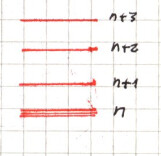
\includegraphics[width=0.15\textwidth]{images/fig_ft2_degeneracion_1.jpg}

Suponemos existe combinación lineal 
\[
	\Ket{0_N^j} = \sum_k a_k^j \Ket{\varphi_N^k}
\]
para escribir un estado degenerado en función de los otros.
\[
	(H_0 - E_N^0 )\Ket{1_N^j} + (V-E_N^{1 j})\Ket{0_N^j} = 0
\]
\[
	\underbrace{\Braket{0_N^j|H_0 - E_N^0|1_N^j}}_{=0} + \Braket{0_N^j|V-E_N^{1 j}|0_N^j} = 0
\]
\[
	\sum_k \Braket{0_N^j|(V-E_N^{1 j})a_k^j|\varphi_N^j} = 0
\]
\[
	\sum_k a_k^j\Braket{0_N^j|V-E_N^{1 j}|0_N^j} = 0
\]
\[
	\sum_k a_k^j\Braket{0_N^j|V|0_N^j} = \sum_k a_k^j\Braket{0_N^j|E_N^{1 j}|0_N^j}
\]
\[
	\sum_k a_k^j\Braket{0_N^j|V|0_N^j} = \sum_k a_k^j E_N^{1 j} \delta_{ik} = a_k^j E_N^{1 j}
\]
Esto último es una ecuación de autovalores y autovectores de la forma:
\[
	(\mathbb{V} - E_N^{1 j} \mathbb{1})\vb{a} =
	0 \qquad \mathrm{det}(\mathbb{V} - E_N^{1 j} \mathbb{1})=0
\]
que permite diagonalizar la matriz de $V$ en la base $\Ket{\vp_n^k}$. Sus autovalores serán las
correcciones $ a_k^j E_N^{1 j} $ de primer orden a la energía. 
\[
	\Braket{0_n^i|V|0_n^j} = E_N^{1 j} \delta_{ij}
\]
Los autoestados $\Ket{1_n^j}$ serán los autovectores del problema.

Hemos roto la degeneración de los estados que estaban degenerados.
Una vez diagonalizado el $V$ estamos en un problema no degenerado; podemos pasar a orden segundo.

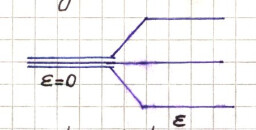
\includegraphics[width=0.4\textwidth]{images/fig_ft2_degeneracion_2.jpg}

\section{Efecto Stark}

Sea un átomo de H con $\Ket{n,\ell,m}$ sin spín y con $n=2$. 
Las soluciones son $\Ket{n,\ell,m}$ con
\[
	0 \leq \ell < n \qquad -\ell \leq m\leq \ell \qquad \ell=0,1 \quad m=-1,0,1
\]

Supongamos $n=2$ con $ E = - e^2 /(8a_0) $, lo cual me lleva a cuatro estados 
\[
	\begin{cases}
	 \Ket{200} \\
	 \Ket{211} \\
	 \Ket{210} \\
	 \Ket{21-1} \\
	\end{cases}
\]
todos con la misma energía $\epsilon_2$.
Consideremos un campo eléctrico en $\hat{z}$ y entonces $V=-ez|\vb{E}|$. 
Luego el potencial se representará por una matriz de $4\times 4$. Sus elementos
serán
\[
	\Braket{n\ell'm'|V|n\ell m} = -e|\vb{E}|\Braket{n\ell'm'|z|n\ell m}
\]
y para evaluarlos usaremos ideas de simetría.

\begin{ejemplo}{\bf refurbished}

Uso un entorno de ejemplo porque la carpeta tiene otra notación y explica más.
\[
	n=2 \to \begin{cases}
	 \ell=0 \qquad 2s \quad & m=0 \; ( 1 \text{ estado}) \\
	 \ell=1 \qquad 2p \quad & m=-1,0,1 \; ( 3 \text{ estados}) 
	\end{cases}
\]
Entonces, las ideas de simetría me llevan a que como son $2s, 2p$ pares
\[
	\Braket{2s|V|2s} = \Braket{2p|V|2p} = 0
\]
y esto son diez elementos nulos. Pero la paridad no nos autoriza a anular $\Braket{2s|V|2p}$.
Como $V \propto z$ y $z \propto T_{q=0}^{k=1}$ sabiendo que
\[
	\Braket{\a',j',m'|T_{q}^{k}|\a, j, m} \propto 
	\Braket{j,k;m,q|j,k;j',m'}
\]
con $m+q=m'$,
lo cual garantiza el teorema de Wigner-Eckart, surge que el único componente no nulo es
\[
	\Braket{2,0,0|V|2,1,0} = 3 e a_0 |E| = \gamma |E|
\]
siendo nulos
\[
	\Braket{2,0,0|V|2,1,\pm 1} = 0
\]
La matriz en la base considerada será [sigue fuera].
 
\end{ejemplo}


$\hat{z}$ es impar ante paridad y entonces vincula estados de paridad diferente,
y entonces 
\[
	\Braket{n\ell m|z|n\ell m} = 0 
\]
\[
	\Braket{n\ell m'|z|n\ell m} = 0 
\]
diagonal nula y con $m'\neq m$ a igual $\ell$ tiene la misma paridad
\[
	\Pi \Ket{2,\ell=1,m} = -\Ket{2,\ell=1,m} \quad \text{impares}
\]
\[
	\Pi \Ket{2,\ell=0,0} = -\Ket{2,\ell=0,0} \quad \text{par}
\]
Solo hay un elemento no nulo correspondiente al producto par-impar.
Se tendrá 
\[
	V = \begin{pmatrix}
	   0 & 0 & 0 & 0 \\
	   0 & 0 & 0 & 0 \\
	   0 & 0 & 0 & \gamma|\vb{E}| \\
	   0 & 0 & \gamma|\vb{E}| & 0
	  \end{pmatrix}
\]
No se podrá romper la degeneración de los estados superiores, todos con cero,
en el subbloque superior de $2\times 2$.
No obstante, se puede diagonalizar considerando estas combinaciones
\[
	\Ket{A} = \frac{1}{\sqrt{2}} \left( \Ket{2,1,0} + \Ket{2,0,0} \right)
	\qquad
	\Ket{B} = \frac{1}{\sqrt{2}} \left( \Ket{2,1,0} - \Ket{2,0,0} \right)
\]
y obtener una matriz
\[
	V = \begin{pmatrix}
	   0 & 0 & 0 & 0 \\
	   0 & 0 & 0 & 0 \\
	   0 & 0 & \gamma|\vb{E}| & 0 \\	   
	   0 & 0 & 0 & \gamma|\vb{E}| 
	  \end{pmatrix}.
\]

En este caso no se rompe la degeneración por completo.
A orden uno aún tenemos dos estados degenerados

	\includegraphics[width=0.5\textwidth]{images/teo2_20.pdf}
	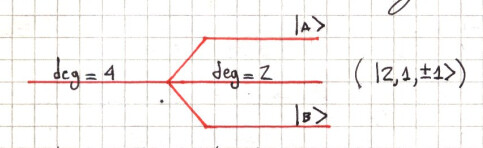
\includegraphics[width=0.5\textwidth]{images/fig_ft2_degeneracion_3.jpg}

Se ha roto parcialmente la degeneración pero si quisiéramos pasar a orden 2 debiéramos
seguir trabajando.

\subsection{Corrimiento de la energía a orden 2 (con degeneración)}

Sea que a orden uno se rompe toda la degeneración 
\[
	(H_0 - E_N^0) \Ket{2_N^j} + (V - E_N^{1 j}) \Ket{1_N^j} - E_N^{2 j} \Ket{0_N^j} = 0
\]
Entonces la corrección a segundo orden de la energía será:
\[
	\Braket{0_N^j | H_0 - E_N^0 | 2_N^j} + \Braket{ 0_N^j | V - E_N^{1 j} | 1_N^j} = E_N^{2 j}
\]
\[
	\Braket{ 0_N^j | V | 1_N^j} = E_N^{2 j}
\]
pues $\Braket{0_N^j|0_N^j}= 0$ pero 
\[
	\Ket{1_N^j} = \sum_{k,i\neq 1} b_k^i \Ket{\varphi_k^i} + \sum_i b_N^i \Ket{\varphi_N^i}
\]
\[
	\Braket{0_N^j|1_N^j} = 0 = \sum_{k,i\neq 1} b_k^i \braket{0_N^j|0_K^i} + 
		\sum_i b_N^i \braket{0_N^j|0_N^i}
\]
falta desarrollo ... [info en mis originaales]

\[
	E_N^{2j} = \sum_{p\neq N} \frac{|\Braket{0_N^j|V|0_p^i}|^2}{E_N^0 - E_p^0}
\]
donde $N$ es un estado degenerado y la suma es entre los $i$ posibles.

\section{Estructura fina del átomo de hidrógeno}

La solución tradicional del átomo de H usa el potencial coulombiano. Esto desemboca en las funciones 
$\Ket{n,\ell,m}$, sin embargo la introducción de ajuste como {\it perturbaciones} rompe algo la degeneración.
\[
	H_0=\frac{p^2}{2m} - \frac{e^2}{r} \qquad E_n = -\frac{\alpha^2m_e^2c^2}{2n^2} \qquad 
	a_0 = \hbar^2/(m_ec^2)
\]
\[
	v/c = p/(mc) = \alpha = \frac{e^2}{\hbar c} \approx 1/137
\]
donde $a_0$ es el radio de Bohr, $\alpha$ es la constante de estructura fina .
Tenemos 
a) Corrección cinemática (relativista)
\[	
	E = c \sqrt{p^2 + m_e^2c^2} = m_ec^2\sqrt{1 + p^2/(m_e^2c^2)} \approx 
	m_ec^2 \left( 1 + \frac{1}{2}\frac{p^2}{m_e^2c^2} + \frac{3}{8}\frac{p^4}{m_e^4c^4} \right)
\]
\[
	E \approx m_ec^2 + \frac{p^2}{2m_e} + \frac{3p^4}{8m_e^3c^2}
\]
y esta corrección va como $W_{mv}/H_0 \sim \alpha^2$.

b) Acoplamiento spín-órbita
Se puede pensar considerando un $e^-$ en reposo con un protón orbitando que genera un $\vb{B}_{eff}$
\[
	W_{so} = \frac{e^2}{2m_e^2c^2} \frac{\vb{L}\cdot\vb{S}}{R^3} = -\vb{\mu}\cdot\vb{B}_{eff}
\]
y la corrección va como $W_{mv}/H_0 \approx \alpha^2$.

c) Término de Darwin o de contacto
\[
	W_D = \frac{\hbar^2}{8m_e^2c^2} \nabla^2 V(r)
\]
que va como  $W_{D}/H_0 \approx \alpha^2$.

Hay otras correcciones hiperfinas que provienen del spín del electrón y del spín del protón. Pero van como 
$\alpha^2/2000$.
Si consideramos el sistema con 
\[
	n=2 \; \ell=0,1 \quad m_\ell = 1,0,-1 \quad m_s=1/2,-1/2
\]
serán ocho estados $\Braket{n,\ell,m_\ell,m_s}$ (base completa).
\[
	W = \underbrace{W_{mv}}_{\sim p^4} + \underbrace{W_{so}}_{\sim \vb{L}\cdot\vb{S}} + 
	\underbrace{W_D}_{\sim |\vb{r}|}
\]
y W es par ante $\Pi$ y sólo habrá elementos de matriz $\neq 0$ que sean de la misma paridad.
\[
	\begin{matrix}
	2s & \qquad 2p \\	 
	\end{matrix}
\]
\[
\begin{matrix}
 2s\\
 2p\\
\end{matrix}
	\begin{pmatrix}
	[2\times 2] & \\
	& [ 6\times 6 ] 
	\end{pmatrix}
\]
$\Ket{2s}$ es par ($\ell=0$) y $\Ket{2p}$ es impar ($\ell=1$) y entonces $\Ket{2s}, \Ket{2p}$
no están conectados.

De manera que hay ocho estados $\Ket{n=2,\ell,m_\ell,s,m_s}$ que al calcular esta perturbación $W$
resultan 
\begin{figure}[htb]
	\begin{center}
	\includegraphics[width=0.9\textwidth]{images/teo2_21.pdf}
	\end{center}
	\caption{}
\end{figure} 

El cálculo para las correcciones hiperfinas no condice la experiencia. Se necesita aquí mecánica cuántica 
relativista. Los dos primeros niveles tienen la misma $\Delta E$ porque en MCR se ve que 
\[
	E = E(n,j) 
\]
es decir que no depende directamente de $\ell,s$.

Un sketch de los métodos perturbativos
\[
	H_0 = \begin{pmatrix}
	       E_1 & \\
	       & E_2 & \\
	       & & E \\
	       & & & E\\
	       & & & & ...\\
	       & & & & & E\\
	       & & & & & & E_3\\
	       & & & & & & & E_4
	      \end{pmatrix}
	      \hspace*{10mm}
	      V =
		\begin{pmatrix}
		& \\
		& \\
		& & V_3 \\
		& & & V_4 \\
		& & & & ... \\
		& & & & & V_{nn} \\
		& \\
		& 
		\end{pmatrix}
\]

En $H$ tenenmos un bloque de energías degeneradas y se diagonalizará el bloque 
correspondiente en la matriz del potencial perturbativo $V$.




% \bibliographystyle{CBFT-apa-good}	% (uses file "apa-good.bst")
% \bibliography{CBFT.Referencias} % La base de datos bibliográfica

\end{document}

	
%  	\input{FT2.c11}
	
%  	\input{FT2.c12}
	
		\documentclass[10pt,oneside]{CBFT_book}
	% Algunos paquetes
	\usepackage{amssymb}
	\usepackage{amsmath}
	\usepackage{graphicx}
% 	\usepackage{libertine}
% 	\usepackage[bold-style=TeX]{unicode-math}
	\usepackage{lipsum}

	\usepackage{natbib}
	\setcitestyle{square}

	\usepackage{polyglossia}
	\setdefaultlanguage{spanish}
	



	\usepackage{CBFT.estilo} % Cargo la hoja de estilo

	% Tipografías
	% \setromanfont[Mapping=tex-text]{Linux Libertine O}
	% \setsansfont[Mapping=tex-text]{DejaVu Sans}
	% \setmonofont[Mapping=tex-text]{DejaVu Sans Mono}

	%===================================================================
	%	DOCUMENTO PROPIAMENTE DICHO
	%===================================================================

\begin{document}

% =================================================================================================
\chapter{Partículas idénticas}
% =================================================================================================

Más apropiado sería partículas indistinguibles. Si en algún punto del espacio se solapan las funciones de 
onda (interfieren) de dos partículas del mismo tipo cosa de que tengan misma masa, carga, etc. (dos 
electrones por ejemplo) no podemos distinguir cual es cual. 

Una tal situación se ilustra en la figura debajo; las dos situaciones son indistinguibles

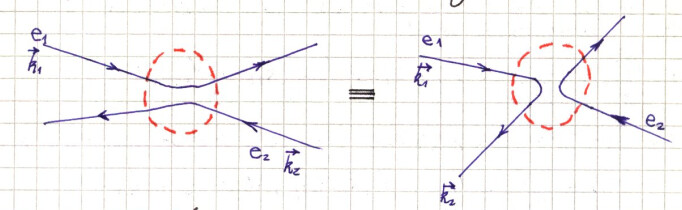
\includegraphics[width=0.65\textwidth]{images/fig_ft2_identical_particles.jpg}

Sean dos estados $\Ket{k'},\Ket{k''}$ con $k^{(i)}$ índice colectivo. 
Si las tengo en una zona común tendré como estado total a $\Ket{k'} \otimes \Ket{k''} $
pero si las partículas son del mismo tipo, 
\[
	\Ket{k'} \otimes \Ket{k''} \qquad \Ket{k''} \otimes \Ket{k'},
\]
representan el mismo sistema cuántico y son ortogonales. No se pueden distinguir estos estados.
\notamargen{No sé si reescribí esta sección diferente a la carpeta porque lo mejoré o si es
equivalente. Se verá en su momento.}

En la zona de interferencia es 
\[
	\Ket{k'}_1 \otimes \Ket{k'}_2 \quad \text{o} \quad \Ket{k''}_1 \otimes \Ket{k''}_2
\]
donde ambos estados son ortogonales y los subíndices numéricos identifican a la partícula. 

\begin{figure}[htb]
	\begin{center}
	\includegraphics[width=0.9\textwidth]{images/teo2_29.pdf}
	\end{center}
	\caption{}
\end{figure} 

	

Entonces un estado general será
\[
	\Ket{K} = c_1 \Ket{k'}_1 \otimes \Ket{k''}_2 + c_2 \Ket{k''}_1 \otimes \Ket{k'}_2
\]
con $|c_1|^2 +|c_2|^2= 1$. 
Esta es la ``degeneración de intercambio'', y la reventaremos con un postulado extra que le
añadiremos a la mecánica cuántica.

Definiremos un operador permutación $P$ que intercambia kets en un producto tensorial.
Es decir que opera según 
\[
	P_{12}( \Ket{k'}_1\otimes \Ket{k''}_2 ) = \Ket{k''}_1\otimes \Ket{k'}_2
\]
y además satisface las siguientes propiedades
\[
	P_{12} = P_{21} \qquad P_{12}^2 = \mathbb{1} \qquad P_{12}^\dagger = P_{12} \qquad 
	P_{12}P_{12}^\dagger = 1 \qquad \text{autovalores:} \; \pm 1
\]

Su función es la de intercambiar etiquetas, no el orden de las partículas.
Sean operadores $\hat{A}_1,\hat{A}_2$ que actúan sobre las partículas 1,2; es decir 
\[
	\hat{A}_1 \equiv \hat{A}_1\otimes\mathbb{1}_2, \qquad 
	\hat{A}_2 \equiv \mathbb{1}_1\otimes\hat{A}_2
\]
Veamos qué sucede sobre autoestados y operadores
\[
	\hat{A}_1 \Ket{a'} \Ket{a''} = a' \Ket{a'} \Ket{a''} \qquad 
	\hat{A}_2 \Ket{a'} \Ket{a''} = a'' \Ket{a'} \Ket{a''} 
\]
\[
	P_{12}A_1P_{12}^{-1}P_{12}\Ket{a'} \Ket{a''} = P_{12} a' \Ket{a'}_1 \Ket{a''}_2 =
	a' \Ket{a''}_1 \Ket{a'}_2
\]
\[
	= P_{12}A_1P_{12}^{-1} \Ket{a''}_1 \Ket{a'}_2 = a' \Ket{a''}_1 \Ket{a'}_2
\]
\[
	= A_2 \Ket{a''}_1 \Ket{a'}_2 = a' \Ket{a''}_1 \Ket{a'}_2
\]
y
\[
	P_{12}\hat{A}_1P_{12}^{-1} = \hat{A}_2, \qquad P_{21} A_1 - A_2 P_{12} = 0
\]
\notamargen{La idea que tenía en la carpeta era la siguiente: si el operador es
simétrico, entonces conmuta con el operador de permutación $P$, no sé si quise
decir eso en las notas de final.}


Luego $\hat{A}$ es simétrico si $[\hat{P}_{12},\hat{A}_{12}]=0$. Sea $[\hat{P}_{12},\hat{H}]=0$ entonces es 
$P_{12}$ constante de movimiento y 
\[
	P_{12} \Ket{\alpha} = \pm \Ket{\alpha}
\]

Un operador que cumple lo de arriba es el hamiltoniano.
Para dos partículas será 
\[
	H = \frac{p_1^2}{2m_1} + \frac{p_2^2}{2m_2} + v(|x_1 - x_2|) + V_e(\vb{x}_1)+ V_e(\vb{x}_2)
\]
donde si las partículas son idénticas se puede hacer $m_1=m_2\equiv m$ y veo que se cumple que
$ [ H, P_{12} ] = 0 $ y $ P_{12} \Ket{\a} = \pm \Ket{\a} $
Defino ahora dos estados, simétrico y antisimétrico
\[
	\Ket{k' k''}_s = \frac{1}{\sqrt{2}}\left( \Ket{k'}_1\Ket{k''}_2 + \Ket{k''}_1\Ket{k'}_2 \right) \qquad 
	\Ket{k' k''}_a = \frac{1}{\sqrt{2}}\left( \Ket{k'}_1\Ket{k''}_2 - \Ket{k''}_1\Ket{k'}_2 \right)
\]
con 
\[
	P_{12}\Ket{\phantom{k}}_s = + \Ket{\phantom{k}}_s \qquad \qquad 
	P_{12}\Ket{\phantom{k}}_a = - \Ket{\phantom{k}}_a
\]
Puedo introducir operadores de simetrización y antisimetrización 
\[
	\hat{S}_{12} \equiv \frac{1}{\sqrt{2}} \left( \mathbb{1} + \hat{P}_{12} \right)
\]
\[
	\hat{A}_{12} \equiv \frac{1}{\sqrt{2}} \left( \mathbb{1} - \hat{P}_{12} \right)
\]
que verifican 
\[
	S^2 = S, \quad  A^2= A, \quad SA=AS=0, \quad [S,A] = 0,
\]
es decir que no son otra cosa que proyectores, 
\[
	\hat{S}_{12} (c_1\Ket{k'}\Ket{k''} + c_2\Ket{k''}\Ket{k'} ) = \frac{1}{\sqrt{2}}(c_1+c_2)
	(\Ket{k'}\Ket{k''} + \Ket{k''}\Ket{k'} )
\]
es simétrico y 
\[
	\hat{A}_{12} (c_1\Ket{k'}\Ket{k''} + c_2\Ket{k''}\Ket{k'} ) = \frac{1}{\sqrt{2}}(c_1-c_2)
	(\Ket{k'}\Ket{k''} - \Ket{k''}\Ket{k'} )
\]
es antisimétrico.
En general se complica bastante con más de dos partículas 
\[
	P_{ij}(\Ket{k'}_1\Ket{k''}_2...\Ket{k^i}_i...\Ket{k^j}_j...) =
	(\Ket{k'}_1\Ket{k''}_2...\Ket{k^j}_i...\Ket{k^i}_j...)
\]
pués tenemos 
\[
	[P_{ij},P_{k\ell}] \neq 0 \quad \text{en general}
\]
Las permutaciones para tres partículas pueden descomponerse en permutaciones de a dos,
como por ejemplo
\[
	P_{123} = P_{12}P_{13} 
\]
\[
	P_{123}\Ket{k'}\Ket{k''}\Ket{k'''} = P_{12}\Ket{k'''}\Ket{k''}\Ket{k'} = \Ket{k''}\Ket{k'''}\Ket{k'}
\]

Con tres partículas hay $3!$ estados; uno totalmente simétrico $\Ket{\phantom{k}}_s$, uno totalmente antisimétrico 
$\Ket{\phantom{k}}_a$ y cuatro sin simetría definida.
Los estados con simetría definida serán 
\begin{align*}
	\Ket{k'k''k'''}_{s/a} = \frac{1}{\sqrt{6}}&\left( \Ket{k'k''k'''} +  \Ket{k''k'''k'} + \Ket{k'''k'k''}\right. \\
	& \left. \pm \Ket{k''k'k'''} \pm \Ket{k'k'''k''} \pm \Ket{k'''k''k'} \right)
\end{align*}
donde el $\Ket{}_a$ tiene el signo $(-)$ en las permutaciones anticíclicas y el $(+)$ en las cíclicas.
Existe un determinante de Slater como método mnemotécnico de obtener los estados $\Ket{}_a$.
\[
	\Ket{ \Psi }_a = \frac{1}{3!}\begin{vmatrix} \; \Ket{k'} & \Ket{k''} & \Ket{k'''} \\  
	\; \Ket{k'} & \Ket{k''} & \Ket{k'''} \\ \; \Ket{k'} & \Ket{k''} & \Ket{k'''} \end{vmatrix}
\]
La obtención de estos estados corresponde a aplicar 
\[
	A_{123} = \frac{1}{\sqrt{3!}}\left( \mathbb{1} + P_{231} + P_{312} - P_{212} - P_{132} - P_{321} \right)
\]
\[
	( \mathbb{1} + P_{23}P_{21} + P_{31}P_{32} - P_{21}P_{23} - P_{13}P_{12} - P_{32}P_{31} )
\]
Si dos $k^{(i)}$ coinciden ya no hay estado antisimétrico posible.

\begin{ejemplo}{\bf Ejercicio 1}

Para la parte a) considera el conjunto $ \{ \Ket{0,-}, \Ket{0,+}, \Ket{1,-}, \Ket{1,+}, ... \} $
que son los $N$ primeros.
Entonces
\[
	E = \sum_{n=0}^{[N/2]-1} \: 2 \hbar \omega \left( n + \frac 1 2 \right) + 
	\hbar \omega \left( \left[ \frac{n}{2} \right] + \frac 1 2 \right)_{\text{ N impar }}
\]

Para la parte b) considero $N=2$ y $ \Ket{0,-} \otimes \Ket{0,+} $ y para ser la función de onda
necesitaré que sea antisimétrica porque son fermiones.
Entonces
\[
	\Ket{\Psi} = \frac{1}{\sqrt{2}}( \Ket{0,-} \otimes \Ket{0,+} - \Ket{0,+} \otimes \Ket{0,-} )
\]
y
\[
	A_{12} ( \Ket{0,-} \otimes \Ket{0,+} ) = \Ket{\Psi}
\]

El hamiltoniano será
\[
	H = \frac{p_1^2}{2m} + \frac{p_2^2}{2m} + \frac{1}{2} m \omega^2 x_1^2
	+  \frac{1}{2} m \omega^2 x_2^2
\]
y entonces
\[
	\Braket{\Psi|H|\Psi} = \frac{1}{2}
	\left( 
	\Bra{0,-} \otimes \Bra{0,+} - \Bra{0,+} \otimes \Bra{0,-}
	\right) H \left( 
	\Ket{0,-} \otimes \Ket{0,+} - \Ket{0,+} \otimes \Ket{0,-}
	\right),
\]
pero com el $H$ no toca los spines entonces serán nulos el primero y el cuarto. Luego
\[
	\Braket{\Psi|H|\Psi} = \frac{1}{2}
	\left(
	\Bra{0,-} \Bra{0,+} H \Ket{0,-}\Ket{0,+} + 
	\Bra{0,+} \Bra{0,-} H \Ket{0,+} \Ket{0,-}
	\right)
\]
y como el $H=H_1+H_2$ cuentas más o menos {\it straighforward} llevan a 
\[
	\Braket{\Psi|H|\Psi} = \hbar \omega.
\]
\notamargen{En la carpeta hay una recarga extra sobre la notación de indicar con un 1 o 2 si
es la primer o segunda partícula; creo que es innecesario, sabemos que el orden de los ket y bra
en esta escritura {\it matters}.}

Ahora queremos calcular el $J^2$ para ello escribamos el estado según
\[
	\Ket{\Psi} = \frac{1}{\sqrt{2}}
	\left( 
	\Ket{0}_1 \otimes \Ket{-}_1 \otimes \Ket{0}_2 \otimes \Ket{+}_2 -
	\Ket{0}_1 \otimes \Ket{+}_1 \otimes \Ket{0}_2 \otimes \Ket{-}_2
	\right)
\]
y reacomodando un poco,
\[
	\Ket{\Psi} = \frac{1}{\sqrt{2}}
	\left( 
	\Ket{0}_1 \otimes \Ket{0}_2 \otimes 
	\left[ \Ket{-}_1  \Ket{+}_2 - \Ket{+}_1 \Ket{-}_2 \right] \right)
\]
y el spin total es nulo, entonces no tenemos dirección privilegiada.
 
\end{ejemplo}

\begin{ejemplo}{\bf Ejercicio 2}

Son dos partículas de spin $3/2$. Por teoría de suma de momentos angulares popdría tener
$3,2,1,0$

\[
	\Ket{j, m} = \sum_{m_1,m_2} \: \Ket{j_1,j_2,m_1,m_2} \Braket{j_1,j_2,m_1,m_2|j,m}
\]
y cuando le aplicamos la permutación
\begin{multline*}
	P_{12} \Ket{j, m} = \sum_{m_1,m_2} \: \Ket{j_2,j_1,m_2,m_1} \Braket{j_1,j_2,m_1,m_2|j,m} = \\
	\sum_{m_1,m_2} \: \Ket{j_1,j_2,m_1,m_2} \Braket{j_1,j_2,m_2,m_1|j,m}
\end{multline*}
vemos que el coeficientes no cambia pero que, puedo sin pérdida de generalidad intercambiar las
letras (son mudas).

Para que sea una función de ferminiones válida necesitaré
\[
	\Braket{j_1,j_2,m_2,m_1|j,m} = - \Braket{j_1,j_2,m_1,m_2|j,m} = (-1)^{j_1+j_2-J} \Braket{}
\]
donde lo último viene de propiedades de los coeficientes.
Luego será $(-1)^{j_1+j_2-J} = -1$ y $3-J$ es natural par.
La simetrización implicará que se acople solamente a spin 2 y spin 0.

\end{ejemplo}

\begin{ejemplo}{\bf Ejercicio 3}
 
Es similar a este. 
 
\end{ejemplo}

\begin{ejemplo}{\bf Ejercicio 4}
 
Misma cuenta, pero para bosones. Llegaremos a $\ell_1 + \ell_2 - L $  para $N$ pares y $2\ell - L$
para $N$ impares.
 
\end{ejemplo}

\begin{ejemplo}{\bf Ejercicio 5}

Vemos solamente la parte b). La base en la cual estamos trabajando es
\[
	\{  \Ket{-1,-1,-1}, \Ket{-1,-1,0}, \Ket{-1,-1,1}, ..., \Ket{1,1,1} \}
\]
y tiene dimensión 27. Estos componentes serán simétricos frente al intercambio de dos partículas.
Por ejemplo para $\Ket{-1,-1,-1}, \Ket{0,0,0}, \Ket{1,1,1}$ es
\[
	\frac{1}{\sqrt{3}} \left( \Ket{-1,-1,0} + \Ket{-1,0,-1} + \Ket{0,-1,-1}  \right)
\]
donde los últimos dos los incluyo para que al intercambiar 1,2 no se altere nada y lo mismo al
intercambiar 2,3.
En general, para los estados que tienen dos repetidos será
\[
	\frac{1}{\sqrt{3}} \left( \Ket{b,b,b} + \Ket{b,a,b} + \Ket{a,b,b}  \right)
\]
que para $a=-1,0,1, b=-1,0,1$ con $a\neq b$ serán seis estados.

Ahora restará cubrir los estados que tienen los tres números distintos, 
\[
	\frac{1}{\sqrt{6}} \left( 
	\Ket{-1,0,1} + \Ket{0,-1,1} + \Ket{1,0,-1} +
	\Ket{1,-1,0} + \Ket{0,1,-1} + \Ket{-1,1,0}
	\right)
\]
y vemos que hay que sumar todos los estaods que tienen una vez cada número.
Ahora tendremos en total $1+3+6$ estados que son simétricos. Los restantes 17 son o bien
antisimétricos o sin simetría definida.

\end{ejemplo}

\section{Postulado de simetrización}

Permitirá romper la degeneración de intercambio. 
Postulamos que toda partícula es de uno de dos tipos de acuerdo a su simetría 

\begin{center}
\begin{tabular}{|c|l|l|l|l|}
\multirow{2}{*}{Sistemas de N part. idénticas} & N & simetrica & BE & entero\\
& N & antisimetrica & FD & semientero
\end{tabular}
\end{center}

\begin{center}
\begin{tabular}{lll}
Función de onda & Estadística & Spin \\
\hline \\
Simétrica & Bosones $P_{ij}\Ket{ N \text{ bosones}} = 
+ \Ket{ N \text{ bosones}} $ & Entero\\
Antisimétrica & Fermiones $P_{ij}\Ket{ N \text{ fermiones}} = 
- \Ket{ N \text{ fermiones}} $ & Semi-entero
\end{tabular}
\end{center}

En la naturaleza no ocurren simetrías mixtas.

% \subsection{Principio de exclusión de Pauli}

Para fermiones, suponiendo un sistema de dos partículas idénticas, es
\[
	\Ket{ \Psi }_a = \frac{1}{\sqrt{2}}( \Ket{k'}_1\Ket{k''}_2 - \Ket{k''}_1\Ket{k'}_2)
\]
y entonces si $k'=k''$ se tiene que 
\[
	\Ket{ \Psi }_a = 0.
\]
de manera que no es posible tener dos fermiones con iguales números cuánticos.
Esto es el principio de exclusión de Pauli. 
Por el contrario los bosones sí pueden tener iguales números cuánticos.

\notamargen{En la carpeta hay un ejemplo que no entiendo en la p81 donde la moraleja
es que el hamiltoniano no tiene modo de vincular estados de bosones con estados de
fermiones. Habría que ver de entenderlo y juzgar luego si aporta introducirlo aquí.}


\subsection{Sistema de dos electrones de spin $1/2$}

Sistema de dos electrones de spin $1/2$, que son fermiones. Sea que el hamiltoniano
no depende del spin total y por ello $[H,S]=0$  con $S = S_1 + S_2$. Se tendrá 
\[
	\Ket{\Psi}^{sist} = \Ket{\Psi}^{spa} \otimes \Ket{\Psi}^{spin},
\]
pero como $\Ket{\Psi}^{sist}$ tiene que ser antisimétrica tendremos 
\[
	P_{12} \Ket{\Psi}^{sist} = - \Ket{\Psi}^{sist} 
\]
que, según la separación anterior, implica que 
\[
	P_{12} \Ket{\Psi}^{sist} = P_{12} \Ket{\Psi}^{spa} \otimes P_{12}\Ket{\Psi}^{spin} 
\]

No obstante, aún antes de saber lo de la parte espacial ya tengo información de la
parte de spin.
Para dos electrones con spin $1/2$ se tiene $j_1+j_2$ entonces $ 0 \leq j \leq 1 $ de modo que $|m_1|\leq j_1$ y
$|m_2|\leq j_2$ entonces $0 \leq S \leq 1$ y $|m_{s_1}|\leq s_1$ y $|m_{s_2}|\leq s_1$.
\[
	\left.\begin{aligned}
	& \Ket{\uparrow \uparrow} \\
	& \Ket{\downarrow \downarrow } \\
	& \frac{1}{\sqrt{2}}( \Ket{ \uparrow\downarrow }+\Ket{ \downarrow\uparrow} )
	\end{aligned}
	\right\} \; \text{triplete} \; s=1 \qquad \text{Estados simétricos}
\]
\[
	\left.\begin{aligned}
	\frac{1}{\sqrt{2}}( \Ket{\uparrow\downarrow} - \Ket{\downarrow\uparrow} )
	\end{aligned}
	\right\} \; \text{singlete} \; s=0 \qquad \text{Estados antisimétricos}
\]

Además se tiene $ [P_{12}, S_\pm] = 0 $ y obtengo los del triplete con la bajada y subida $S_\pm$,
de modo que todos están relacionados.
Luego, $ P_{12} \ket{\Psi}^{spin} $ será simétrico $S=1$ o antisimétrico $S=0$ y esto es 
independiente del hamiltoniano $H$ y viene de que pudimos separar parte espacial y spin.

Ahora bien, como simétrico por antisimétrico en $S\otimes A$ es antisimétrico
\[
	P_{12} \Ket{\Psi}_{sist} =
	P_{12}^{spa} \Ket{\Psi}_{spa} \otimes P_{12}^{spi} \Ket{\Psi}_{spin}
\]
y se tienen en cada caso $A \otimes S$ en $S=1$ o bien $S \otimes A$ en $S=0$ será
en el primer caso $\Ket{\Psi}_{spa}$ antisimétrica con $(-1)^\ell$ y $\ell$ impar 
y en el segundo caso $\Ket{\Psi}_{spa}$ simétrica con $(-1)^\ell$ y $\ell$ par. 


Entonces
\begin{gather*}
	\begin{aligned}
	s=0 \qquad \Rightarrow \; &\Ket{\Psi}^{spa} \text{es simétrica} \\
	s=1 \qquad \Rightarrow \; &\Ket{\Psi}^{spa} \text{es antisimétrica}
	\end{aligned}	
\end{gather*}	

Vistos desde el centro de masa dos electrones verifican que $ P_{12} = \Pi $ 
(el operador $P_{12}$ es paridad) y entonces
\notamargen{Dos electrones solo pueden acoplarse a impulso total par $\vb J = \vb L + \vb S$.
Acá hay un mix de explicaciones, evidentemente carpeta no coincidía con las notas.}
\[
	P_{12}\Ket{n\ell m} = (-1)^\ell \Ket{n\ell m}
\]
\[
	\ell \;\text{par} \; \rightarrow \Ket{\Psi}^{spa} = P_{12} \Ket{\Psi}^{spa} \qquad 
	\ell \;\text{impar} \; \rightarrow -\Ket{\Psi}^{spa} = P_{12} \Ket{\Psi}^{spa}
\]
Necesitaré $\ell$ par con $s=0$ entonces $\ell+s=j$ par. En cambio, si $\ell$ impar con $s=1$ entonces 
$\ell+s=j$ par. Dos electrones sólo se acoplan a momento total $j$ par.

Podemos poner los siguientes estados 
\[
	\Ket{ \Psi }_{sa} = \frac{1}{\sqrt{2}}( \Ket{k'}\Ket{k''} \pm \Ket{k''}\Ket{k'})
\]

Teniendo una relación $A\Ket{a_i} = a_i \Ket{a_i}$ para un operador $A$, 
un autoestado con una partícula con autovalor $a_1$ y otra con $a_2$ se escribe
\[
	\Ket{ \Psi_F }_{sa} = \frac{1}{\sqrt{2}}( \Ket{a'}\Ket{a''} \pm \Ket{a''}\Ket{a'}),
\]
donde habrá que simetrizar o antisimetrizar si las partículas son bosones o fermiones,
respectivamente. Usando $ \text{Prob}_{(a_1,a_2)} = | _{S/A}\Braket{\Psi_f|\Psi}_{S/A} |^2 $,
la probabilidad será
\begin{multline*}
	\text{Prob}\; = |_{sa}\Braket{\Psi|\Psi}_{sa}|^2 =  \\
	\left|\frac{1}{2}(_1\Bra{a'}_2\Bra{a''} \pm _1\Bra{a''}_2\Bra{a'})(\Ket{k'}_1\Ket{k''}_2 \pm 
	\Ket{k''}_1\Ket{k'}_2)\right|^2 =
\end{multline*}
\begin{multline*}
 	= \frac{1}{4}\left| \Bra{a'}\Bra{a''}\Ket{k'}\Ket{k''} \pm \Bra{a''}\Bra{a'}\Ket{k'}\Ket{k''} 
	\right. \pm \\
	\left. \Bra{a'}\Bra{a''}\Ket{k''}\Ket{k'} \pm \Bra{a''}\Bra{a'}\Ket{k''}_1\Ket{k'} \right|^2 \\
	= \frac{1}{4}\left| 2\Braket{a'|k'}\Braket{a''|k''} \pm 2\Braket{a''|k'}\Braket{a'|k''}\right|^2, 
\end{multline*}
que se puede escribir como
\[
	\text{Prob}\; = \left| \underbrace{\Braket{a'|k'}\Braket{a''|k''}}_{\text{término directo}} \pm 
	\underbrace{\Braket{a''|k'}\Braket{a'|k''}}_\text{término de intercambio}\right|^2
\]
donde hemos marcado un término directo y uno de intercambio, asociado con la probabilidad de que una
partícula pase al estado de la otra. El signo $+$ es para bosón y el signo $-$ para fermión. El término 
directo asocia entonces $k_1 \to a_1$ y $k_2 \to a_2$ mientras que el de intercambio $k_1 \to a_2$ y 
$k_2 \to a_1$.

Al explicitar la cuenta con el módulo al cuadrado obtenemos la interferencia (de sentido cuántico) que
aparece porque son indistinguibles las partículas
\begin{multline*}
	\text{Prob}\; = |_{sa}\Braket{\Psi|\Psi}_{sa}|^2 = \left| \Braket{a'|k'}\Braket{a''|k''} \right|^2 + 
	\left|\Braket{a''|k'}\Braket{a'|k''}\right|^2  \\
	\pm 2\mathcal{Re}\left(\underbrace{ \Braket{a'|k'}\Braket{a'|k''}^*\Braket{a''|k''}\Braket{a''|k'}^* 
	}_\text{Interferencia}\right)
\end{multline*}

Vemos que aparece una interferencia que será importante solamente si hay solapamiento. En el caso de no 
solaparse o con partículas clásicas sólo el primer término es de importancia.

Esto puede aplicarse al caso ilustrativo de la ``teleportación''.
Consideremos el ejemplo de medición de electrones en lugares apartados, como

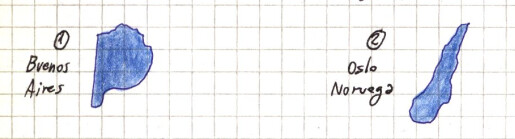
\includegraphics[width=0.6\textwidth]{images/fig_ft2_extra_identical.jpg}

En Buenos Aires tenemos $\psi_1 = \Braket{\vbx | k_1} \neq 0 $ y $\psi_2 = \Braket{\vbx | k_2} = 0 $
mientras que en Oslo $\psi_1 = 0 $ y $\psi_2 \neq 0 $ lo que significa que el electrón de Oslo en $\psi_2$
no lo puedo hallar en Buenos Aires.
Luego, $\Braket{\vbx|a_1}\neq 0 $ y $\Braket{\vbx|a_2} = 0 $ siendo la primera la variable dinámica asociada
al detector en Buenos Aires.


\section{El átomo de helio}

Posee dos protones, dos neutrones y dos electrones. La figura bajo estas líneas ilustra el sistema
coordenado

\includegraphics[width=0.4\textwidth]{images/teo2_30.pdf}

El hamiltoniano se puede escribir 
\[
	H = \frac{p_1}{2m} + \frac{p_2}{2m} - \frac{2e^2}{r_1} -  \frac{2e^2}{r_2} + \frac{e^2}{r_{12}}
\]
y si el último término es $\sim 0$ decimos que en ese caso $H$ está desacoplado y tenemos una
función de onda del tipo
\[
	\Psi = \Psi_1 \otimes \Psi_2.
\]
Dado que se verifica
\[
	[\vb{H},\vb{S}] = 0 
	\qquad 
	\vb{S} = \vb{S}_1 + \vb{S}_2 = 
	\begin{cases} 
	0 \\ 
	1 
	\end{cases}
\]
se da que $S$ es constante de movimiento y para la $\Ket{\psi_{spin}}$ se tiene 
\[
	S=0 \qquad \frac{1}{\sqrt{2}}( \Ket{ \uparrow\downarrow }-\Ket{ \downarrow\uparrow}) \quad \text{singlete}
\]
\[
	S=1 \qquad \begin{aligned}
	& \Ket{\uparrow \uparrow} \\
	& \Ket{\downarrow \downarrow } \\
	& \frac{1}{\sqrt{2}}( \Ket{ \uparrow\downarrow }+\Ket{ \downarrow\uparrow} )
	\end{aligned} \quad \text{triplete}
\]
Sea un electrón  en el estado fundamental $ \Ket{100}$ y otro en algún estado excitado $ \Ket{n\ell m}$,
se tendrán
\[
	\Ket{\Psi}_{He} = \frac{1}{\sqrt{2}}\left(  \Ket{100}\Ket{n\ell m} \pm  \Ket{n\ell m}\Ket{100}
	\right) \Ket{\Psi_{spin}}
\]
donde el signo $+$ es para $S=0$ y el signo $-$ para $S=1$ y vemos que $\Ket{\Psi_{spin}}$ tiene simetría
bien definida.
Así, con $S=0$, será
\[
	\Ket{\Psi}_{He} = \frac{1}{\sqrt{2}}\left( \Ket{100}\Ket{n\ell m} + \Ket{n\ell m}\Ket{100}\right) 
	\frac{1}{\sqrt{2}}( \Ket{ \uparrow\downarrow }-\Ket{ \downarrow\uparrow})
\]
y en cambio con $S=1$
\[
	\Ket{\Psi}_{He} = \frac{1}{\sqrt{2}}\left(  \Ket{100}\Ket{n\ell m} - \Ket{n\ell m}\Ket{100}\right) 
			\begin{cases}
	                   \Ket{\uparrow \uparrow} \\
			   \Ket{\downarrow \downarrow } \\
			   \frac{1}{\sqrt{2}}( \Ket{ \uparrow\downarrow }+\Ket{ \downarrow\uparrow} )
	                  \end{cases} .
\]
\notamargen{Lo que uno simetriza o antisimetriza son las partículas idénticas.}

Ahora introduzcamos la interacción con el término $e^2/r_{12}$. Consideremos, en teoria de perturbaciones,
que 
\[
	E_{He} = E_{100} + E_{n\ell m} + \Delta E
\]
donde 
\[
	\Delta E = \Braket{\Psi|\frac{e}{r_{12}}|\Psi}
\]
y el término en el {\it sandwich} lo considero una perturbación.
Haciendo la cuenta explícitamente
\begin{multline*}
	\Delta E = \Bra{\Psi^{spin}}^\dagger \frac{1}{2}\left(\Bra{100}\Bra{n\ell m} \pm \Bra{n\ell m}\Bra{100}
	\right) \frac{e}{r_{12}} \times \\
	\left(\Ket{100}\Ket{n\ell m} \pm \Ket{n\ell m}\Ket{100}\right)\Ket{\Psi^{spin}}
\end{multline*}
\[
	\Delta E = \Bra{100}\Bra{n\ell m}\frac{e}{r_{12}}\Ket{100}\Ket{n\ell m} \pm  
	\Bra{n\ell m}\Bra{100}\frac{e}{r_{12}}\Ket{100}\Ket{n\ell m}
\]
donde vemos que el operador es invariante antes $1 \to 2, 2 \to 1$ pués $|\vbx_1 - \vbx_2| = |\vbx_2 - \vbx_1| 
\equiv r_{12}$ y que escribiremos más resumidamente como
\[
	\Delta E = I \pm J.
\]

Para calcular necesitaremos integrar metiendo una identidad
\[
	\int d^2x_1 d^2x_2 \: \Bra{100}\Bra{n\ell m}\frac{e}{r_{12}} \left[ 
	\Ket{x_1}\Ket{x_2} \Bra{x_1}\Bra{x_2}
	\right] \Ket{100}\Ket{n\ell m}
\]
tras lo cual, luego de un amasaje veríamos que
\[
	I = \int d^2x_1 d^2x_2 \: \frac{e}{r_{12}} \:
	|\Psi_{100}(x_1)|^2 |\Psi_{n\ell m}(x_2)|^2
\]
\[
	J = \int d^2x_1 d^2x_2 \: \frac{e}{r_{12}} \: 
	\Psi_{100}(x_1) \Psi_{n\ell m}(x_2) \Psi_{100}(x_2)^* \Psi_{n\ell m}(x_1)^*
\]

En un diagrama ilustrativo sería algo como

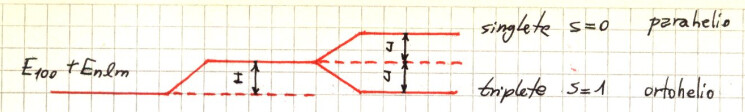
\includegraphics[width=0.8\textwidth]{images/fig_ft2_extra_identical2.jpg}

\begin{figure}[htb]
	\begin{center}
	\includegraphics[width=1.0\textwidth]{images/teo2_15.pdf}
	\end{center}
	\caption{}
\end{figure} 

Vemos un efecto debido al spin de las partículas que no está en el hamiltoniano (puesto que
el $H$ no depende del $\vb S$).
Esta separación de los niveles en $\pm J$ se debe al carácter de fermión de las partículas.
Es una consecuencia de la simetría de la función de onda.

\begin{ejemplo}{\bf Ejercicio 7}

[Este es simplemente un {\it sketchi}]

Como $S=0$ entonces son bosones y $P\Ket{m} = \Ket{m}$. Entonces
\[
	P_{(1\to 2,2\to 3, 3\to 1)} = D_R(2\pi/3,\hat{z})
\]
de manera que $D_R\Ket{m} = \Ket{m}$ lo cual lleva a que $\euler^{ - i / \hbar J_z 2\pi /3 } \Ket{m}$
que será
\[
	\euler^{ - i / \hbar J_z 2\pi /3 } \Ket{m} = \Ket{m}
\]
por lo tanto $\euler^{-i 2\pi m / 3} = 1$ que lleva a $n = m/3 \in \mathbb{Z}$ luego $m=3n$ que
son múltiplos de $n$. Los valores de $J_z$ serán $3\hbar, 6\hbar, 9\hbar, ...$.

\end{ejemplo}

\begin{ejemplo}{\bf Ejercicio 8}

Son dos fermiones, $s=1/2$ y consecuentemente $\Psi_T$ entonces como 
$\Psi_{T} = \Psi_{spa}(\vbx_1, \vbx_2, \vbx_3) \Psi_{spin}$ necesito que $\Psi_{spa}$ sea antisimétrica.

\end{ejemplo}

\begin{ejemplo}{\bf Ejercicio 9}

Consideramos tres partículas de spin 1 que son bosones. La función de onda $\Psi$ total debe ser
simétrica ante el intercambio.
Luego, como
\[
	\Psi_{T} = \Psi_{spa}(\vbx_1, \vbx_2, \vbx_3) \Psi_{spin}
\]
la función $\Psi_{spin}$ debe ser simétrica.

En el apartado i) tendremos
\[
	\begin{cases}
	 1 & \Ket{+} \\
	 2 & \Ket{+} \\
	 3 & \Ket{+} 
	\end{cases}
	\qquad 
	\Ket{+ + +} = \Psi_{spin}
\]
y el spin total es 3.

En ii) tenemos
\[
	\begin{cases}
	 1 & \Ket{+} \\
	 2 & \Ket{+} \\
	 3 & \Ket{0} 
	\end{cases}
	\qquad 
	\Ket{+ + 0}, \Ket{+0+}, \Ket{0++} \qquad 
	\Psi_{spin} = \frac{1}{\sqrt{3}}(\Ket{+ + 0} + \Ket{+0+} + \Ket{0++})
\]

Mientras que en iii) las tres partículas están con estado de spin diferente $\Ket{+}, \Ket{0} ,\Ket{-}$
de manera que hay una regla de construcción que es tipo determinante
\[
	\begin{bmatrix}
	 \Ket{+}_1 & \Ket{0}_1 & \Ket{-}_1 \\
	 \Ket{+}_2 & \Ket{0}_2 & \Ket{-}_2 \\
	 \Ket{+}_3 & \Ket{0}_3 & \Ket{-}_3 
	\end{bmatrix}
\]
pero aún hay que establecer los signos específicos.
Entonces
\[
	\Psi_{spin} = \frac{1}{\sqrt{6}} \left[ 
	\Ket{+ 0 - } + \Ket{+ - 0 } + \Ket{0 + - } + 
	\Ket{0 - +} + \Ket{- + 0} + \Ket{- 0 + }
	\right] 
\]

La parte b) nos dice que $ \Psi_{T} = \Psi_{spa}(\vbx_1, \vbx_2, \vbx_3) \Psi_{spin} $ pero ambas
son antisimétricas. Tenemos
\[
	\Psi_{spin} = \begin{cases}
	 \Ket{+ +} \\
	 \Ket{- -} \\
	 1/\sqrt{2} ( \Ket{+ -} + \Ket{- +} )
	\end{cases},
\]
que son simétricas. Consideramos un pozo de ancho $L$ de modo que $\Psi_n = A \sin( k_n x )$ para la
cual las energías correspondientes serán $E_n m^2 \hbar^2 \pi^2 /( 8^ m2 L )$ y si intercambio las
dos partículas $ \Psi_1(\vbx_1) \Psi_1(\vbx_2) $ veo que falla.
La parte espacial no puede estar en 11. Las necesitaré en estados diferentes. Entonces si $m_1, m_2$
son el 1,2 tendré
\[
	\Psi_{spa}^A = \frac{1}{\sqrt{2}}( \Psi_1(\vbx_1) \Psi_2(\vbx_2) - \Psi_1(\vbx_2) \Psi_2(\vbx_1) )
\]
que al hacer un intercambio vemos que saca un signo menos afuera de modo que es antisimétrica.

La parte b) involucra $ \Psi_T = \Psi_{spa} \Psi_{spin} $ antisimétrica y $1/\sqrt{2}(\Ket{+-} - \Ket{-+})$
que llevan a
\[
	E = E_1 + E_2 = ( 1^2 + 2^2 ) \frac{\hbar^2 \pi^2 }{ 8 m^2 L}
\]
de modo que la función total es
\[
	\Psi_T = \frac{1}{\sqrt{2}} \Psi_1(x_1) \Psi(x_2)( \Ket{+-} - \Ket{-+}).
\]

\end{ejemplo}



% \bibliographystyle{CBFT-apa-good}	% (uses file "apa-good.bst")
% \bibliography{CBFT.Referencias} % La base de datos bibliográfica

\end{document}

	
		\documentclass[10pt,oneside]{CBFT_book}
	% Algunos paquetes
	\usepackage{amssymb}
	\usepackage{amsmath}
	\usepackage{graphicx}
% 	\usepackage{libertine}
% 	\usepackage[bold-style=TeX]{unicode-math}
	\usepackage{lipsum}

	\usepackage{natbib}
	\setcitestyle{square}

	\usepackage{polyglossia}
	\setdefaultlanguage{spanish}
	



	\usepackage{CBFT.estilo} % Cargo la hoja de estilo

	% Tipografías
	% \setromanfont[Mapping=tex-text]{Linux Libertine O}
	% \setsansfont[Mapping=tex-text]{DejaVu Sans}
	% \setmonofont[Mapping=tex-text]{DejaVu Sans Mono}

	%===================================================================
	%	DOCUMENTO PROPIAMENTE DICHO
	%===================================================================

\begin{document}




% =================================================================================================
\chapter{Picture de interacción y perturbación dependiente del tiempo}
% =================================================================================================

Estudiaremos perturbaciones dependientes del tiempo 
\[
	H = H_0 + V(t), \qquad H_0 \Ket{n} = E_n \Ket{n} \; (\text{ datos})
\]
donde, no obstante, $\Ket{n}$ no dependiente del tiempo. 
La idea es que hasta $t=0$ no hay potencial $V$ y luego al {\it encenderse} el potencial el estado pasará
a otro
\[
	\Ket{i} \longrightarrow \Ket{j}.
\]

Se estudiarán transiciones entre autoestados del mismo hamiltoniano $H_0$ (que son estacionarios). 
Un autoestado permanece en el tiempo como tal pero con fase oscilante (como veremos).
\notamargen{Esta deducción está diferente de la carpeta, confío en que sea una versión depurada.
Se la analizará en la próxima fase. En la página 75 y 76 en la práctica hay un resumen de toda
la formulación.}
Usamos una representación de interacción y definimos
\[
	\Ket{\alpha,t_0,t}_s = \euler^{-iH/\hbar(t-t_0)}\Ket{\alpha,t_0}_s
\]
\[
	= \euler^{-iH/\hbar(t-t_0)} \euler^{-iV(t)/\hbar(t-t_0)} \Ket{\alpha,t_0}
\]
\[
	= \sum_n \euler^{-iH_0/\hbar \: t} \euler^{-iV(t)/\hbar \: t} \ket{n}\Braket{n|\alpha,t_0}
\]
\[
	= \sum_n \euler^{-iE_n^0/\hbar \: t }\ket{n}\euler^{-iV(t)/\hbar \: t } \Braket{n|\alpha,t_0}	
\]
\[
	\euler^{iH_0/\hbar t}\Ket{\alpha,t_0,t}_s =
	\sum_n  \underbrace{\euler^{-iV(t)/\hbar \: t} \Braket{n|\alpha,t_0}}_{C_n(t)} \ket{n} = \Ket{\alpha,t_0,t}_I	
\]
es decir que se escriben los kets como
\[
	 \Ket{\alpha,t_0,t}_I = \euler^{iH_0/\hbar t}\Ket{\alpha,t_0,t}_s.
\]
Aquí se puede pensar que 
\begin{itemize}
 \item $C_n(t)$ evoluciona por $V(t)$
 \item $\euler^{-iE_n^0 t/\hbar}$ evoluciona por $H_0$
\end{itemize}

Esto introduce la {\it picture} (o representación) de Dirac, también llamada ``de interacción'', en la 
cual los estados evolucionan con $V(t)$.
La siguiente tabla compara con las anteriores [atrasarla porque lo de los operadores aparece después]
\begin{center}
\begin{tabular}{|c|ccc|}
\hline 
& Dirac & Schrödinger & Heinsenberg \\
\hline 
% & &  & \\
estados & evolucionan & evolucionan & fijos \\
$\Ket{\alpha}$ & con $V(t)$ & con $H$ &  \\
\hline
operadores & evolucionan & fijos & evolucionan \\
 & con $H_0$ &  & con $H$ \\
\hline
base & fijos & fijos & evolucionan \\
$\Ket{a'}$ &  &  &  \\
\hline 
% & & & \\
\end{tabular}
\end{center}

\[
	i\hbar \dpar{}{t}\Ket{\alpha,t_0,t}_s = H \Ket{\alpha,t_0,t}_s
\]
\[
	i\hbar \dpar{}{t}\left( \euler^{-iH_0t/\hbar}\Ket{\alpha,t_0,t}_I \right) = 
	H \euler^{-iH_0t/\hbar} \Ket{\alpha,t_0,t}_I
\]
\[
	i\hbar \euler^{-iH_0t/\hbar}\dpar{}{t} \Ket{\alpha,t_0,t}_I = 
	V(t) \euler^{-iH_0t/\hbar} \Ket{\alpha,t_0,t}_I
\]
\[
	i\hbar \dpar{}{t} \Ket{\alpha,t_0,t}_I = V(t) \Ket{\alpha,t_0,t}_I,
\]
que es la ecuación de evolución de los kets, y es equivalente a la ecuación de Schrödinger.

La definición debe verificar asimismo que 
\[
	_s\Braket{\; A_s \;}_s = _I\Braket{\; A_I \;}_I,
\]
lo cual conduce a
\begin{multline*}
	_I\Braket{\alpha,t_0,t|A_I|\alpha,t_0,t}_I = \\
	_s\Braket{\alpha,t_0,t|\euler^{-iH_0t/\hbar}A_I\euler^{iH_0t/\hbar}|\alpha,t_0,t}_s = 
	_s\Braket{\alpha,t_0,t|A_s|\alpha,t_0,t}_s,
\end{multline*}
o bien a que los operadores evolucionan según 
\[
	A_I = \euler^{iH_0t/\hbar}A_s\euler^{-iH_0t/\hbar}
\]
\[
	\dtot{A_I}{t} = \frac{1}{i\hbar}[A_I, H_0]
\]
que es igual que la ecuación de Heisenberg pero con $\hat{H}_0$ en lugar de $H$.
Los kets base permanecen fijos, porque así lo hacen en Schrödinger, en realidad oscila su fase; entonces 
\[
	\Ket{n,t_0,t}_s = \euler^{-iHt/\hbar} \ket{n,t_0}_s
\]
\[
	\Ket{n,t_0,t}_I = \euler^{iH_0t/\hbar} \euler^{-iHt/\hbar} \ket{n,t_0}_s =
	\euler^{-iVt/\hbar} \ket{n,t_0}_s = \euler^{iH_0t/\hbar} \ket{n,t_0}_s
\]
\[
	\Ket{n,t_0,t}_I = \euler^{iE_0t/\hbar} \ket{n,t_0,t}_s
\]
\notamargen{En la carpeta está primero lo de los kets base y luego la ecuación de movimiento 
que acá aparece inmediatamente debajo de la tabla. Aquí habrá que reordenar material.}

Finalmente, resta ver qué le sucede a los coeficientes.

\[
	\Ket{\alpha,t_0,t}_I = \sum_n \Ket{n}\Braket{n|\alpha,t_0,t}_I = \sum_n C_n(t) \Ket{n}
\]
\[
	C_n(t) = \euler^{iVt/\hbar} \Braket{n|\alpha,t_0}_s
\]
\[
	\Braket{n|\alpha,t_0,t}_I = C_m(t)
\]
con $\Ket{n},\ket{m}$ autoestados de $H_0$, le pego un $\Bra{n}$ a la ecuación de evolución de kets,
\[
	i\hbar \dpar{}{t} \Braket{n|\alpha,t_0,t}_I = \Braket{n|V_I(t)|\alpha,t_0,t}_I
\]
\[
	= \sum_m \Braket{n|V_I(t)|m}\Braket{m|\alpha,t_0,t}_I
\]
\[
	i\hbar \dpar{}{t}C_n(t) = \sum_m C_m(t) \Braket{n|V_I(t)|m}
\]
\[
	i\hbar \dpar{}{t}C_n(t) = \sum_m C_m(t) \Braket{n|V_s|m} \euler^{it(E_n-E_m)/\hbar}
\]
\be
	i\hbar \dpar{}{t}C_n(t) = \sum_m C_m(t) V_{nm}(t) \euler^{i\omega_{nm}t}
	\label{solu_sistema}
\ee
donde $V_{nm}(t) \equiv \Braket{n|V(t)|m}$ y $\omega_{nm} \equiv (E_n-E_m)/\hbar$.
Esta es la ecuación que cumplen los coeficientes, donde $|C_n(t)|^2$ es la probabilidad de hallar al sistema 
en el autoestado $\Ket{n}$.
Resolver esto puede ser muy difícil, salvo en los casos en que es tan fácil que no nos
sirve de nada \footnote{Esto es un patrón que se observa a menudo en física teórica.}.
En efecto, la \eqref{soluc_sistema} es un sistema de ecuaciones diferenciales acopladas.
Esto puede ponerse en forma matricial como
\[
	i\hbar \begin{pmatrix}
	\dot{c}_1 \\ \dot{c}_2 \\ ... \\ \dot{c}_N \\
	\end{pmatrix} 
	=
	\begin{pmatrix}
	V_{11} & V_{12}\euler^{i\omega_{12}} & ... \\ 
	V_{21}\euler^{i\omega_{21}} & V_{22} & ... \\ 
	... \\ 
	... \\
	\end{pmatrix}
	\begin{pmatrix}
	c_1 \\ c_2 \\ ... \\ c_N \\
	\end{pmatrix} .
\]


\subsection{Método perturbativo (dependiente del tiempo)}

Pensaremos en una serie perturbativa 
\[
	C_n(t) = C_n(t)^{(0)} + C_n(t)^{(1)}  + C_n(t)^{(2)}  + ...
\]

El evolucionador temporal en la picture de interacción cumple 
\[
	\Ket{\alpha,t_0,t} = U_I(t,t_0)\Ket{\alpha,t_0}_I, \qquad t > t_0
\]
que viene de  
\[
	i\hbar \dtot{}{t} U_I(t,t_0) = V_I(t) U_I(t,t_0)
\]
con $U_I(t_0,t_0)=\mathbb{1}$, la cual resolviendo nos hace llegar a 
\[
	U_I(t,t_0) = \mathbb{1} - \frac{i}{\hbar}\int_{t_0}^{t} V_I(t')U_I(t',t_0) dt'.
\]

Esta ecuación debe proporcionarnos la forma de hallar $U_I$. Se puede usar una iteración sencilla
\[
	U_I(t,t_0) = \mathbb{1} - \frac{i}{\hbar} \int_{t_0}^t \: V_I(t') \left[ 
	\mathbb{1} - \frac{i}{\hbar} \int_{t_0}^t \: V_I(t'') U_I(t'',t_0) dt''
	\right] \: dt',
\]
\[
	U_I(t,t_0) = \mathbb{1} - \frac{i}{\hbar} \int_{t_0}^t \: V_I(t') \left[ 
	\mathbb{1} - \frac{i}{\hbar} \int_{t_0}^t \: V_I(t'') \left(
	\mathbb{1} - \frac{i}{\hbar} \int_{t_0}^t \: V_I(t''') \left\{ ... \right\} dt''
	\right) dt''
	\right] \: dt',
\]
y esto lleva a la serie de Dyson, casi una expresión formal,
\begin{multline*}
	U_I(t,t_0) = \mathbb{1} - \frac{i}{\hbar}\int V_I(t') dt' + \left( -\frac{i}{\hbar} \right)^2\int_{t_0}^t 
	V_I(t') \int_{t_0}^{t'}V_I(t'')dt'' + ...\\ + \left( -\frac{i}{\hbar} \right)^n 
	\int_{t_0}^t dt'\int_{t_0}^{t'}dt''\int_{t_0}^{t''}dt''' ... \int_{t_0}^{t^{n-1}}dt^{n} V_I(t') 
	V_I(t'')...V_I(t^n)	
\end{multline*}
que es una especie de exponencial $ \euler^{T[-i/\hbar \int V(t) dt ]}$.

La serie de Dyson puede verse como un desarrollo perturbativo.

\subsection{Transiciones entre autoestados del hamiltoniano $H_0$}

Veamos el detalle de las transiciones en el formalismo de Dirac.
\[
	\Ket{i,t_0=0,t}_I = U_I(t,0) \Ket{i} = \sum_n \Ket{n}\Braket{n|U_I(t)|i}
\]
y como se viera oportunamente
\[
	\Ket{i,t}_I = \sum_n C_n(t)\Ket{n} = \sum_n \left( \Braket{n|U_I(t)|i} \right) \Ket{n}.
\]
La amplitud de transición será 
\[
	C_n(t) = \Braket{n|U_I(t)|i}
\]
con $\Ket{i},\Ket{n}$ autoestados de $H_0$.
Sea $\tilde{C}_n(t)=\Braket{n|U_s(t)|i}$, donde vemos que $\tilde{C}_n(t)$ y $C_n(t)$ difieren en
una fase, y busquemos una expresión 
\[
	\Ket{\alpha, t_0, t}_I = \euler^{iH_0t/\hbar} \Ket{\alpha, t_0, t}_s
\]
\[ 
	= \euler^{iH_0t/\hbar} U_S(t,t_0)\Ket{\alpha, t_0}_s
\]
\[
	\Ket{\alpha, t_0, t}_I  = \euler^{iH_0t/\hbar} U_S(t,t_0) \euler^{-iH_0t_0/\hbar}  \Ket{\alpha, t_0}_I
	= U_I(t,t_0) \Ket{\alpha,t_0}_I
\]
\[
	\euler^{iH_0t/\hbar} \hat{U}_S \euler^{-iH_0t_0/\hbar} = \hat{U}_I
\]
y notemos que $\hat{U}$ no obedece la ley de transformación de operadores.

\[
	C_n(t) = \Braket{n|\euler^{iH_0t/\hbar} U_S(t,t_0) \euler^{-iH_0t_0/\hbar}|i}
\]
\[
	C_n(t) = \euler^{-i/\hbar[E_n^{(0)} t - E_i^{(0)} t_0]} \Braket{n| U_S(t,t_0) |i} =
		\euler^{-i/\hbar[E_n^{(0)} t - E_i^{(0)} t_0]} \tilde{C}_n(t)
\]
lo que lleva a 
\[
	|C_n(t)|^2 = |\tilde{C}_n(t)|^2.
\]
Para transiciones entre autoestados de $H_0$ los coeficientes dan la misma probabilidad 
(evaluados con el evolucionador de Dirac que con el de Schrödinger).
Debe notarse que esto se cumple siempre y cuando la transición sea entre autoestados del
hamiltoniano y la fase resulte así global.


Veamos las transiciones 
\[
	\Braket{ n | U_I(t,t_0)| i }
\]
a los diferentes órdenes en la perturbación
\begin{itemize}
 \item orden 0
 \[
	C_n^{(0)}(t) = \Braket{n|1|i} = \delta_{ni}
 \]
 \item orden 1
 \[
 	C_n^{(1)}(t) = -\frac{i}{\hbar} \int_{t_0}^t \euler^{i\omega_{ni} t'} V_{ni}(t') dt' \qquad \qquad 
 	V_{ni} \equiv \Braket{n|V(t)|i}
 \]
 \item orden 2
 \[
 	C_n^{(2)}(t) = \sum_m \left( -\frac{i}{\hbar} \right)^2  \int_{0}^t  dt'\int_{0}^t dt''
 	\euler^{it'/\hbar(E_n-E_m)} V_{nm}(t') \euler^{it''/\hbar(E_m-E_i)} V_{mi}(t'')
 \]
\end{itemize}
y entonces la probabilidad de ir desde $\ket{i} \to \Ket{n}$ con $i\neq n$, hasta orden dos, sería
\[
	P^{(2)}_{i\to n} = |C_n^{(0)}(t)+C_n^{(1)}(t)+C_n^{(2)}(t)|^2 =
	| C_n^{(1)}(t) + C_n^{(2)}(t) |^2
\]
donde debe notarse que hay interferencia entre los diversos términos.

\begin{ejemplo}{\bf Sobre observación en práctica}

Había anotado como conclusión en el resumen dado en la práctica que a primer orden solo hay transiciones
entre estados consecutivos. A segundo orden solo hay transiciones hasta el segundo consecutivo (esto se
ve claro en los diagramas de Feynmann).
Luego, aclaré que esto no es cierto en general y que hay que mirar el potencial $V(t)$.
 
\end{ejemplo}

\begin{ejemplo}{\bf Ejercicio 12}

Consideramos el siguiente
\[
	H = H_0 + F_0 x \cos (\omega t), \qquad \qquad 
	H_0 \Ket{n} = \hbar \omega \left( n + \frac 1 2 \right), \Ket{i} = \Ket{0}
\]
con $\Braket{n|V(t)|0} = F_0 \cos(\omega t) \Braket{n|x|0}$. Escribimos $x$ en función de $a,a^\dagger$
con lo cual solamente sobrevive $n=1$
\[
	\Braket{1|V(t)|0} = F_0  \cos(\omega t) \sqrt{ \frac{\hbar}{2 m \omega_0 } }
\]

Tenemos $C_0^{(0)}(t)=1$ y $C_1^{(0)}(t)=0$ que significa que no hay transición cuando estamos en un
autoestado de $H$.
Luego, $C_0^{(1)}(t)=0$ y para 
\[
	C_1^{(1)}(t) = - \frac{i}{\hbar} \int_{t_0}^t \: \euler^{i (E_1 - E_0) t' / \hbar } \:
	\sqrt{ \frac{\hbar}{2 m \omega_0 } } \: F_0 \cos(\omega t') \: dt'
\]
y esto da algo.
Escribo
\[
	\Ket{\psi(t)}_I \approx ( C_0^{(0)} + C_0^{(1)}  ) \Ket{0} + ( C_1^{(0)} + C_1^{(1)} ) \Ket{1}
	= \Ket{0} + C_1^{(0)}(t) \Ket{1}
\]
Este estado no está normalizado porque es una aproximación a orden dado donde no se han tirado los
subsiguientes términos, lo cual está bien porque es una aproximación. Si normalizase otra vez quedo
con un problema diferente. Piden calcular $\vm{x}$.
\[
	\vm{x} = _I\Braket{\psi(t)| \euler^{i H_0 t/\hbar} x \euler^{-i H_0 t/\hbar} |\psi(t)}_I
	= \Braket{\psi(t)| U_I^+ \euler^{i H_0 t/\hbar} x \euler^{-i H_0 t/\hbar} U_I |0}
\]
Resulta
\[
	C_1^{0} = \frac{i F_0 }{\sqrt{ 2 \hbar m \omega_0 } (\omega - \omega_0)}
\]
y si $\omega - \omega_0$ es cercano a cero me alejo demasiado de la normalización del estado y entonces
en realidad no tiene mucho sentido el método perturbativo.
Vale con coeficientes pequeños: si los coeficientes son grandes estaré tirando una cosa de norma grande
y no tiene sentido.

\end{ejemplo}


\subsection{Ejemplo: potencial constante encendido abruptamente}

Sea un potencial que prendemos y apagamos luego, pero constante. Es decir
\[
	V(t) = \begin{cases}
	0 	& t < 0  \\
	V(r,p,s,L,...) & t \geq 0
	\end{cases}
\]
donde $V \neq V(t)$, pero puede depender de cualquier otra cosa. La figurilla más abajo
ilustra este {\it escalón}.

\includegraphics[width=0.45\textwidth]{images/teo2_22.pdf}

A orden cero no vemos cambio pues
\[
	C^0_n(t) = 0.
\]
A orden uno es 
\[
	C^1_n(t) = -\frac{i}{\hbar} \int_0^t \euler^{i/\hbar(E_n - E_i)t'} V_{ni} \: dt'=
	\frac{V_{ni}}{(E_n - E_i)}(1-\euler^{i\omega_{ni}t})
\]
donde debemos notar que si esto revienta porque $E_n \sim E_i$ entonces la teoría de
perturbaciones no puede usarse aquí.

Evaluando la probabilidad se tiene	
\[
	|C^1_n(t)|^2 = 
	\frac{4|V_{ni}|^2}{| E_n - E_i|^2}\sin^2\left(\frac{(E_n - E_i)t}{2\hbar}\right).
\]

	\includegraphics[width=0.45\textwidth]{images/fig_ft2_potencial_abrupto.jpg}

Es máxima la probabilidad cuando $\Delta E\to 0$. 
En ese caso las transiciones son a estados de la misma energía. 
El gráfico de arriba es a un dado $t$ fijo. A medida que el tiempo transcurre el gráfico
tiende a una delta de Dirac.

A tiempo largo la probabilidad es no nula para aquellos estados 
\[
	t \sim \frac{2\pi}{|\omega_{ni}|}
\]

Hay probababilidad de transición $\Ket{i} \to \Ket{n}$ apreciable donde $\omega = \frac{2\pi}{t}
= \frac{\Delta E}{\hbar}$ dado que $\Delta t \Delta E \sim \hbar $. O bien, $\Delta E \sim 0$.

\section{Scattering}

Podemos pensarlo como el caso de un potencial que se prende y apaga, representando éste el objeto
contra el cual se hace scattering.

\includegraphics[width=0.6\textwidth]{images/fig_ft2_scattering_intro.jpg}

Este último ejemplo puede aplicarse a colisiones elásticas. Prendemos y apagamos un potencial que es el 
masacote al cual impactamos. De entrada ha partículas libres y de salida (lejos de $V$) partículas libres.
Entonces $ E_n - E_c \sim 0$ y consideraremos lo que sucede a tiempos largos. Interesará la probabilidad 
total de transicionear a estados de energía similares a $E_i$. Por ello se considera 
\be
	\sum_{\substack{n \\ E_n\sim E_i}} |C^1_n(t)|^2 
	\longrightarrow 
	\int \: \rho(E_n) \: |C^1_n(t)|^2 \: dE_n
	\label{scattering_integral}
\ee
donde el integrando es el número de estados dentro de un intervalo de energías $(E,E+dE)$ a los cuales
se puede transicionar. Esta erá la probabilidad de transición.

\begin{figure}[htb]
	\begin{center}
	\includegraphics[width=0.6\textwidth]{images/teo2_23.pdf}
	\end{center}
	\caption{}
\end{figure} 

A primer orden la probabilidad será algo como
\[
	\lim_{t\to\infty} \; \int \: \rho(E_n) \: \frac{4|V_{ni}|^2}{| E_n - E_i|^2}
	\sin^2\left(\frac{(E_n - E_i)t}{2\hbar}\right) \: dE_n,
\]
puesto que estamos considerando lo que sucede a tiempos muy largos.
En esos casos, como la probabilidad tiende a una delta de Dirac, 
\[
	\lim_{t\to\infty} \frac{1}{| E_n - E_i|^2}
	\sin^2\left(\frac{(E_n - E_i)t}{2\hbar}\right) = \frac{\pi t}{2\hbar} \delta(E_n - E_i),
\]
la integración es fácil y se obtiene
\[
	\lim_{t\to\infty} \; \int \: \rho(E_n) |C^1_n(t)|^2 \: dE = 
	\left.\left(\frac{2\pi}{\hbar}\right) \rho(E_n) |\bar{V}_{ni}|^2 \: t \: \right|_{E_n\sim E_i}
\]
donde $\bar{V}_{ni}$ es un potencial promedio. La probabilidad de transición es proporcional a $t$. 

Se suele definir una tasa de transición (probabilidad de transición por unidad de tiempo)
\[
	\dtot{}{t}\left( \sum_{\substack{n \\ E_n\sim E_i}} |C_n^{(1)}|^2 \right) =
	\left(\frac{2\pi}{\hbar}\right)	|\bar{V}_{ni}|^2 \rho(E_n) = \omega_{i\to n}^{(1)}
\]
que es la regla de oro de Fermi, y sirve para calcular cualquier transición entre estados
para potenciales que no dependen del tiempo.

[reacomodar]
La energía al final se mide con cierto error $\Delta E$ de modo que se obtendrá $E \pm \Delta E$ y 
deberá sumar [no sé bien qué se quiere decir acá]
\[
	\sum_n | C_n(t) |^2 \quad (E_n \sim E \pm \Delta E)
\]
Pero si no es discreto necesitaré integrar (la integral \eqref{scattering_integral})

\section{El método variacional}

Se puede usar para aproximar la energía del estado fundamental (el estado de energía mínima).
No conocemos $\Ket{n}$ ni $E_n$, pero $ H \Ket{n} = E_n \Ket{n}$ donde $\{ \Ket{n} \}$ es
una base.
Evaluamos
\[
	\Braket{\psi|H|\psi} = \sum_{n,m}\Braket{\psi|n}\Braket{n|H|m}\Braket{m|\psi} =
		\sum_{n,m} E_n \Braket{\psi|n}\Braket{n|m}\Braket{m|\psi} 
\]
\[
	\Braket{\psi|H|\psi} = \sum_{n,m} E_n C_n^*\Braket{n|m}C_m = \sum_{n} E_n|C_n|^2
\]
\[
	\sum_{n} E_n|C_n|^2 \geq \sum_n E_0|C_n|^2 = E_0 \sum_n |C_n|^2 = E_0 \Braket{\psi_n|\psi_n}
\]
y usamos 
\[
\Ket{\psi} = \sum_n \Braket{n|\psi}\Ket{n} \qquad \Bra{\psi} = \sum_n \Braket{\psi|n}\Bra{n} 
\]
para arribar a
\[
	\frac{\Braket{\psi_n|H|\psi_n}}{\Braket{\psi_n|\psi_n}} \geq E_0.
\]
donde $E_0$ es la energía más baja. Esto no parece ser muy iluminador que digamos.
Se considera que $\psi$ es tal que 
\[
	\Braket{x|\psi} = \psi(x)_{|x|\to\infty} \to 0
\]
lo que significa que la función de onda es {\it well behaved} (bien comportada).

\begin{ejemplo}{\bf Ejercicio 10}

A partir de $ \Braket{x|\psi} = \euler^{-\b|x|}$ se tiene, intercalando la completitud,
\[
	\Braket{\psi|\psi} = 
	\int_{-\infty}^\infty \: \Braket{\psi | x'}\Braket{x' | \psi} \: dx' = 
	2 \int_{-\infty}^\infty \: \euler^{- 2 \b |x| } \: dx = \frac{1}{\b}
\]
y del mismo modo
\begin{multline*}
	\Braket{\psi|H|\psi} = \Braket{\psi| \frac{p^2}{2 m} + \frac{m \omega^2 x^2 }{2} |\psi} = \\
	- \Frac{\hbar^2}{2m} \int_{-\infty}^\infty \: 
	\dtot[2]{}{x}\left( \Braket{\psi|x} \right)\Braket{x'|\psi} \: dx' +
	\frac{m\omega^2}{2} \int_{-\infty}^\infty \: \Braket{\psi|x^2|x'} \Braket{x'|\psi} \: dx',
\end{multline*}
para finalmente
\[
	\Braket{\psi|H|\psi} = - \Frac{\hbar^2}{2m} \int_{-\infty}^\infty \: 
	\dtot[2]{}{x}\left( \euler^{- \b |x| } \right) \euler^{- \b |x| } \: dx' +
	\frac{m\omega^2}{2} \int_{-\infty}^\infty \: \euler^{- 2 \b |x| } x^2 \: dx'
\]

Trabajaremos por partes esta cosa. Una integral con la doble derivada se convierte en
\[
	\int_{-\infty}^\infty \: u \dtot[2]{u}{x} \: dx = 
	\left. u \: \dtot{u}{x} \right|_{-\infty}^\infty - \int_{-\infty}^\infty \: \Dtot{u}{x}^2 \: dx
\]
donde el primer término es nulo porque la función de onda es bien comportada.
Con este enfoque resulta
\[
	\Braket{\psi|H|\psi} = - \frac{\hbar^2 \b}{2m} + \frac{m\omega^2}{4\b^3},
\]
y entonces \notamargen{Typo seguro.}
\[
	\mathcal{E}(\psi) = \b \left( - \frac{\hbar^2 \b}{2m} + \frac{m\omega^2}{4\b} \right) \geq E_0 
\]
y entonces desde
\[
	\left. \dpar{\mathcal E}{\b}\right|_{\b_{\text{min}}} = 0
\]

El único parámetro libre es $\b$; entonces se calcula el $\beta$ que hace minimo esta cosa y ya está
resuelto.
 
\end{ejemplo}

\begin{ejemplo}{\bf Ejercicio 11}

Tenemos la siguiente ecuación:
\[
	\dtot[2]{\psi}{x} + (\lambda -|x|)\psi = 0,
\]
con $\psi \to 0$ si $|x|\to\infty$. Se tiene
\[
	\begin{cases}
	 C(\a - |x|) & |x|\leq \a \\
	 0 & |x| > \a
	\end{cases}
\]

Para el hamiltoniano en cuestión es
\[
	\left[ \right] \Ket{\psi} = \mathcal E \Ket{\psi},
\]
que conduce a la ecuación
\[
	- \frac{\hbar^2}{2m} \dtot[2]{\psi}{x} + V(x)\psi = \mathcal E  \psi
\]
la cual reescribimos como
\[
	\dtot[2]{\psi}{x} + 
	\left[ \frac{2m}{\hbar^2} \mathcal E - \frac{2m}{\hbar^2} V(x) \right] \psi  = 0
\]
e identificamos a ojo que
\[
	V(x) = \frac{\hbar^2}{2m}|x|, \qquad \lambda = \frac{2m\mathcal E}{\hbar^2}
\]
de manera que habría que minimizar $\lambda$ haciendo mínimo $\mathcal E$ respecto de $\a$.
 
\end{ejemplo}

\begin{ejemplo}{\bf Ejercicio 7}

Estamos en el átomo de hidrógeno. Es decir $\Ket{n,\ell,m}$ donde $n \in \mathbb N$, $\ell < n$
y $-\ell \leq m \leq \ell$.

Tendremos
\begin{eqnarray*}
 n=1 \qquad & \Ket{1 0 0 } \\
 n=2 \qquad & \Ket{211}, \Ket{210}, \Ket{21-1}, \Ket{200}
\end{eqnarray*}
donde los primeros tres del orden dos son $\Ket{2p} = \Ket{21m}$ y el último es $\Ket{2s}$.
La perturbación requerirá una matriz de $5\times5$ y habrá que diagonalizar $E_2^{(1)}$, que
es el bloque inferior (ver iluscración).
La perturbación es algo del tipo $V = - e E z $

\includegraphics[width=0.5\textwidth]{images/fig_ft2_ejercicio7A.jpg}

Tenemos
\[
	\Braket{2 \ell m|-eEz|2\ell' m'} = -e E \Braket{2\ell m|z|2\ell' m'}
\]
y como el operador paridad cumple $\Pi z \Pi^{-1} = -z$ se da
\[
	\Pi \Ket{n\ell m} = (-1)^\ell \Ket{n\ell m}
\]
lo cual no es otra cosa que usar reglas de selección. Luego,
\[
	\Braket{2\ell m|-z|2\ell' m'} = (-1)^{\ell+\ell'} \Braket{2\ell m|z|2\ell' m'}
\]
y si $\ell+\ell'=L$ entonces el braket es nulo y sobreviven $\ell\neq \ell'$ de modo que
$\Braket{21m|z|200}$ es el que permanece.

Por Wigner-Eckart $z=T_0^1$ de modo que
\[
	\Braket{\a' j' m'|T_q^k|\a j m} = И \Braket{j k m q|j k j' m'}
\]
donde $И$ es una constante. Entonces
\[
	\Braket{21m|T_0^1|200} = И \Braket{0100 | 011m }
\]
desde lo cual sobreviven $\Braket{0100|011m}$ si $m=0$.

Entonces se tiene lo que ilustra la imagen

\includegraphics[width=0.5\textwidth]{images/fig_ft2_ejercicio7B.jpg}

y como es una matriz de Pauli su diagonalización es un juego de niños. Se tienen
\[
	\Ket{v_1} = \frac{1}{\sqrt{2}} \left( \Ket{200} + \Ket{210} \right)
	\qquad \qquad 
	\Ket{v_2} = \frac{1}{\sqrt{2}} \left( \Ket{200} - \Ket{210} \right)
\]

Si se cambia de base y se escribe el potencial $V$ en la base $\{ \Ket{100}, \Ket{v_1}, 
\Ket{v_2}, \Ket{211}, \Ket{21-1} \}$ se tiene

\includegraphics[width=0.5\textwidth]{images/fig_ft2_ejercicio7C.jpg}

que es una matriz diagonal por bloques. 
 
\end{ejemplo}

\subsection{Scattering a orden dos y OFPT}

Para el coeficiente a orden 1 teníamos la regla de oro de Fermi.
El coeficiente a orden dos es
\[
	C_n^{(2)} = \Frac{-i}{\hbar}^2 \sum_{m \neq i} V_{nm} V_{mi}
	\int_0^t \: dt' \: \euler^{ i \omega_{nm} t'} 
	\int_0^{t'} \: dt'' \: \euler^{ i \omega_{ni} t''}
\]
donde la integral más interna se aproxima como
\[
	\frac{i}{\omega_{mi}} \left[ 1 - \euler^{ i t' \omega_{mi} } \right]
\]
y eso nos permite considerar el siguiente límite
\[
	\lim_{t \to \infty} C_n^{(2)} = 
	\frac{i}{\hbar} \: \sum_{m \neq i} \: \frac{V_{nm} V_{mi}}{E_n - E_i}
	\int_0^t \: dt' \: ( \euler^{ i \omega_{ni} t'} - \euler^{ i \omega_{nm} t'} ),
\]
de manera que a orden dos es
\[
	\omega_{i\to n}^{(2)} = \frac{2\pi}{\hbar}\left. \left| \overline{ V_{ni} + \sum_{m\neq i} 
	\frac{V_{nm}V_{mi}}{(E_i-E_m)}} \right|^2 \rho(E_n) \right|_{E_n\sim E_i}.
\]

Para obtener los siguientes términos dentro del $\bar{||^2}$ podemos emplear un ardid gráfico conocido como 
{\it Old Fashioned Perturbation Theory}, que no es más que un artilugio diagramático mnemotécnico.

Consideramos un caso como el scattering de una zona donde existe un potencial al que bombardeamos con
partículas en estados $\Ket{i}$ y que salen partículas con estados $\Ket{n}$ de la misma energía.
Ver figura inicial en Fig siguiente.

\includegraphics[width=1.0\textwidth]{images/teo2_24.pdf}

Luego, el estado $\Ket{m}$ es un pseudoestado virtual que no conserva la energía y es un artificio surgido
del cálculo (ver figura intermedia). El segmento entre los vértices es un {\it propagador} y de alguna manera
podemos hacernos la idea de que transporta la perturbación entre vértices. Cada uno de los vértices es
un elemento de matriz.

\includegraphics[width=0.6\textwidth]{images/fig_ft2_tre_ordenes_perturbativos.jpg}

Podríamos avanzar con este grafismo y especular con lo que sucede a tercer orden. Este término será sumar
sobre todos los caminos posibles
\[
	\sum_{m,j \neq i, m \neq j} V_{nj} \frac{1}{E_j - E_m} 
	V_{jm} \frac{1}{E_m - E_i} V_{mi}.
\]

Estos diagramas son los que llevan el nombre de OFPT. Es importante notar que implica que entre los
estados intermedios estados virtuales $\Ket{m},\Ket{j}$ no se conserva la energía; son propagadores.
La energía se conserva solo en el inicial y el final. Si la energía se conservase reventarían los
denominadores.

Consideremos ahora una perturbación armónica dada en términos de un potencial escrito de forma
hermítica
\[
	V(t) = \mathbb{V} \euler^{i\omega t} + \mathbb{V}^\dagger \euler^{-i\omega t},
		\qquad \mathbb{V}\neq \mathbb{V}(t)
\]
Encendemos este potencial y queremos pasar de estados $\Ket{i} \to \Ket{n}$ viendo su probabilidad de 
transición a orden uno,
\[
	C_n^{(1)}(t) = -\frac{i}{\hbar} 
	\int_0^t ( V_{ni}\euler^{i\omega t'}+ V_{ni}^\dagger \euler^{-i\omega t'} )
	\euler^{i\omega_{ni}t'}dt'
\]
donde la diferencia con un potencial constante es el primer término del paréntesis [?]. Entonces,
\[
	C_n^{(1)}(t) = -\frac{i}{\hbar} \left[ V_{ni} \int_0^t \euler^{i(\omega +\omega_{ni})t'} dt' + 
		V_{ni}^\dagger \int_0^t \euler^{i(-\omega +\omega_{ni})t'} dt' \right]
\]
\[
	C_n^{(1)}(t) = -\frac{i}{\hbar} \left[ V_{ni} 
	\frac{\euler^{i(\omega +\omega_{ni})t} -1}{i( \omega +\omega_{ni} )}
	+ V_{ni}^\dagger \frac{\euler^{i(-\omega +\omega_{ni})t} - 1}{i(-\omega +\omega_{ni})} \right]
\]
\[
	C_n^{(1)}(t) = \frac{V_{ni}}{\hbar} \frac{1-\euler^{i(\omega +\omega_{ni})t}}{( \omega +\omega_{ni} )}
	+ \frac{V_{ni}^\dagger}{\hbar} \frac{1-\euler^{i(-\omega +\omega_{ni})t}}{(-\omega +\omega_{ni})}
\]
donde se ve que el primer término es similar a $\delta(\omega_{ni} +\omega)$ y el segundo a
$\delta(\omega_{ni} - \omega)$ de suerte que
\[
	\lim_{t\to\infty} C_n^{(1)}(t) = \frac{1}{\hbar}\left[ V_{ni}\delta(\omega_{ni}+\omega) 
		+ V_{ni}^\dagger \delta(\omega_{ni}-\omega) \right]
\]
Esto representa $E_n = E_i - \hbar \omega$ en el primer término y $E_n = E_i + \hbar \omega$ en el segundo
que pueden asociarse a la emisión de un cuanto de energía en la interacción o a la absorción, respectivamente.

\includegraphics[width=0.4\textwidth]{images/fig_ft2_perturbativos_1a.jpg}
\includegraphics[width=0.4\textwidth]{images/fig_ft2_perturbativos_1b.jpg}

Entonces todo el término representa la probabilidad de emitir o absorber fotones.
Veamos el ejemplo de emisión o absorción que ocurre en un átomo.

\includegraphics[width=0.4\textwidth]{images/fig_ft2_perturbativos_2a.jpg}
\includegraphics[width=0.4\textwidth]{images/fig_ft2_perturbativos_2b.jpg}

Los $V,V^\dagger$ se puede asociar como que aniquilan o crean fotones.
Otro asunto es que al descomponer un campo EM en Fourier tengo las frecuencias $\omega$ separadas
y debería sumar entre todas las frecuencias, pero se ve que no es necesario y la única que debo
considerar es [4] (número dentro de la figura!).

Luego será nulo sólo si 
\[
	\omega_{ni} = -\omega \qquad \longrightarrow \qquad 
		\frac{E_n - E_i}{\hbar} = -\omega \quad E_n = E_i - \hbar\omega
\]
\[
	\omega_{ni} = -\omega \qquad \longrightarrow \qquad 
		\frac{E_n - E_i}{\hbar} = \omega \quad E_n = E_i + \hbar\omega
\]

\begin{figure}[htb]
	\begin{center}
	\includegraphics[width=1.0\textwidth]{images/teo2_25.pdf}
	\end{center}
	\caption{}
\end{figure} 

Luego, $ \lim_{t\to\infty} C_n^{(1)}(t) $ representa la probababilidad de emitir o absorber 
fotones en una interacción. Se puede asociar que $V$ crea fotones y $V^\dagger$ destruye fotones. 
Para un átomo se tiene 

\begin{figure}[htb]
	\begin{center}
	\includegraphics[width=1.0\textwidth]{images/teo2_26.pdf}
	\end{center}
	\caption{}
\end{figure} 

En teoría de perturbaciones de dos partículas vemos que a orden $n$ se intercambian $n$ fotones.

\includegraphics[width=0.4\textwidth]{images/fig_ft2_perturbativos_3a.jpg}
\includegraphics[width=0.4\textwidth]{images/fig_ft2_perturbativos_3b.jpg}

En el gráfico de la izquierda a primer orden los impulsos están determinados mientras que a orden
dos, en el gráfico de la derecha, no sabemos el impulso $q$ y debiéramos integrar pero la integral
da infinito
\[
	\lim_{\Lambda \to \infty} \int_{-\Lambda}^\Lambda \: dq.
\]
Feymann desarrolló una ``renormalización'' que tapa estos infinitos considerando que hay que usar
una serie perturbativa para la carga $e$ en los vértices.

Todo este formalismo permite la aparición de partículas y antipartículas. Aquí $\Delta t = t_2 - t_1$ es
tan chico que 
\[
	\Delta t \Delta E \sim \hbar
\]

\includegraphics[width=0.4\textwidth]{images/fig_ft2_desdoblamiento_1a.jpg}

La joda es que la ``cosa de abajo'' 

\includegraphics[width=0.4\textwidth]{images/fig_ft2_desdoblamiento_1b.jpg}

es equivalente pero podemos sumarlo para obtener

\includegraphics[width=0.4\textwidth]{images/fig_ft2_desdoblamiento_2a.jpg}

que es ocurrencia de Feynmann, pero el propagador es un fotón virtual y puede tener masa.

Este formalismo se puede aplicar directamente también al electromagnetismo. Sea una corriente $j^\mu(x,t)$
que genera un potencial $A^\mu$; se puede calcular con un ``propagador''
\[
	A^\mu(x',t') = \int dx dt \: G^\mu(x,t ; x', t') j^\mu(x,t)
\]
donde la función de Green oficia de propagador para llevar la interacción de $x',t'$ a $x,t$.
Luego, $j_{2\mu}(x',t') A^\mu(x',t')$ es proporcional a la fuerza entre corrientes.
\[
	\int dx dt \: j_{2\mu}(x,t) G^\mu_\nu(x,t ; x', t') j^\nu_1(x,t)
\]

Podemos pensar en un diagramita donde a primer orden se intercambia un fotón

\includegraphics[width=0.3\textwidth]{images/fig_ft2_desdoblamiento_2b.jpg}

\subsection{Despoblamiento de estados iniciales}

Suponemos que pasamos entre estados $\Ket{i} \to \Ket{i}$ (número de estados).
Queremos ver con qué velocidad $v$ se despoblan los $\Ket{i}$. 
Para elllo me construyo un potencial {\it suave}
\[
	\lim_{\eta\to 0} V(t) = \euler^{\eta t} \mathbb{V}, \qquad  \mathbb{V} \; \text{ cte.}
\]
donde $\eta$ es un parámetro regularizador, cuyo fin es regularizar divergencias que
puedan aparecer en el denominador.

\begin{figure}[htb]
	\begin{center}
	\includegraphics[width=0.5\textwidth]{images/teo2_27.pdf}
	\includegraphics[width=0.4\textwidth]{images/fig_ft2_desdoblamiento_3.jpg}
	\end{center}
	\caption{}
\end{figure} 

Partamos de $ \Ket{i} \to \Ket{n} $
\[
	C_n^{(1)}(t) = \lim_{t\to\infty} -\frac{i}{\hbar} 
	\int_{t_0}^t V_{ni} \euler^{\eta t'} \euler^{i\omega_{ni} t'} dt' =
	-\frac{i}{\hbar} V_{ni} 
	\frac{\euler^{\eta t} \euler^{i\omega_{ni} t} }{\eta+i\omega_{ni}}
\]
y consecuentemente
\[
 	|C_n^{(1)}(t)|^2 = \frac{|V_{ni}|^2}{\hbar^2} 
 	\frac{\euler^{2\eta t} }{\eta^2 + \omega_{ni}^2 }.
\]
La variación temporal será
\[
	\dtot{}{t}|C_n^{(1)}(t)|^2 = 2 \eta \frac{|V_{ni}|^2}{\hbar^2} \frac{\euler^{2\eta t} }{\eta^2 + \omega_{ni}^2 }
\]
y tomando el límite $\eta \to 0$ 
\[
	\lim_{\eta\to 0} \dtot{}{t}|C_n^{(1)}(t)|^2 = 2 \frac{|V_{ni}|^2}{\hbar^2} 
			\frac{\eta }{\eta^2 + \omega_{ni}^2 } = \begin{cases}
	                    0 \quad \text{si}\;\; \omega_{ni}^2 \neq 0 \\
	                    \infty \quad \text{si}\;\; \omega_{ni}^2 = 0
	                   \end{cases}
\]
y llegamos a la regla de oro de Fermi,
\[
	\dtot{}{t}|C_n^{(1)}(t)|^2 = 2 \frac{|V_{ni}|^2}{\hbar^2} \delta(\omega_{ni}) \pi.
\]

Veamos ahora qué sucede cuando $n=i$. Se tienen $C_i^{(0)}(t) = 1$ y [?]
\[
	C_i^{(0)}(t) = - \frac{i}{\hbar} \lim_{t_0 \to -\infty}
	\int_{t_0}^t \: V_{ii} \euler^{\eta t '} dt' = -\frac{ i }{\hbar \eta } V_{ii}\euler^{\eta t}
\]
\[
	C_i^{(2)}(t) = \Frac{-i}{\hbar}^2 \sum_m |V_mi|^2 \lim_{t_0\to\infty}
	\int_{t_0}^t \: dt' \: \euler^{i \omega_{im} t' + \eta t' }
	\frac{\euler^{i \omega_{mi} t' + \eta t' }}{ i ( \omega_{mi} - i \eta ) }
\]
mientras que si dividimos la sumatoria en $m$ se tiene ahora
\[
	= \left( -\frac{i}{\hbar} \right)^2 \frac{|V_{ii}|^2 \euler^{2\eta t}}{2\eta^2}
	- \frac{i}{\hbar} \sum_{m\neq i} \frac{|V_{mi}|^2 \euler^{2 \eta t}}{ 2 \eta ( E_i - E_n + i \hbar \eta ) }
\]

Hasta orden dos tenemos
\[
	C_i(t) = C_i^{(0)}(t) + C_i^{(1)}(t) + C_i^{(2)}(t)
\]
y
\[
	\frac{1}{C_i(t)} \dtot{C_i(t)}{t} = 
	\frac{ 
	-\frac{i}{\hbar} V_{ii} 
	+ \left( -\frac{i}{\hbar} \right)^2 \frac{|V_{ii}|^2 \euler^{\eta t}}{\eta}
	- \frac{i}{\hbar} \sum_{m\neq i} \frac{|V_{mi}|^2 \euler^{2 \eta t}}{E_i - E_n + i \hbar \eta }
	}
	{
	1 - \frac{i}{\hbar \eta} V_{ii} \euler^{\eta t} + C_i^{(2)}(t)
	}
\]
\notamargen{Acá usamos un Taylor para dividir por $1+e$ y así multiplicar por $1-e$... Taylor, pelotudo.}
pero no necesito poner el $C_i^{(2)}(t)$ puesto que al hacer el cociente me generarán términos
cúbicos que tiraré; por ello no lo considero.
Haciendo la cuenta a segundo orden en teoría de perturbaciones de $\eta \to 0$ obtenemos un
límite finito. Tendiendo
\[
	\frac{1}{C_i(t)} \dtot{C_i(t)}{t} = -\frac{i}{\hbar}
	\left[ 
	V_{ii} + \sum_{m\neq i} \frac{|V|^2}{E_i - E_n + i \hbar \eta }
	\right] = -\frac{i}{\hbar} \Delta_i
\]
que implica la ecuación diferencial 
\[
	\dtot{C_i(t)}{t} = - \frac{i}{\hbar} \Delta_i C_i(t)
\]
cuya solución es por supuesto $ C_i(t) = \euler^{- i \Delta_t t / \hbar } $.
Ahora se tiene que la evolución temporal lleva 
\[
	\Ket{i} \longrightarrow C_i(t) \euler^{-i E_i t /\hbar} \ket{i} = 
	\euler^{i (E_i -\Delta i) t / \hbar } \Ket{i}
\]
mientras que a primer orden $ E_i \to E_i + V_{ii}$.

Analicemos el término
\[
	\frac{1}{E_i - E_n + i \hbar \eta}
\]
teniendo en cuenta que en análisis complejo se sulen separar 
\[
	\lim_{\epsilon \to 0 } \frac{1}{x + i  \epsilon} = P_p\left[ \frac{1}{x}\right] - i \pi \delta(x)
\]
y luego, la
\[
	\sum_{m\neq i} \frac{|V|^2}{E_i - E_n + i \hbar \eta }
\]
se descompondrá en una parte real y en una imaginaria, donde esta última representará la difusión con
el tiempo que cobrará importancia si $ E_i = E_n $ y entonces
\[
	C_i^{(2)}(t) = \euler^{- i/\hbar \mathfrak{Re}(\Delta_i) t  + 1/\hbar \mathfrak{Im}(\Delta_i) t}
\]

Se suelen definir el ancho de decaimiento
\[
	\frac{\Gamma_i}{\hbar} = - \frac{2}{\hbar}\mathfrak{Im}(\Delta_i)
\]
de modo que
\[
	|C_i^{(2)}(t)|^2 = \euler^{ - \Gamma_r t /\hbar} = \euler^{ - t/\tau_i}
\]
donde $\tau_i = \hbar / \Gamma_i$. La componente compleja da el decaimiento, como en electromagnetismo,
y también da información de la variación del número de estados $\Ket{i}$

\section{Scattering sección eficaz}

Emplearemos teoría de perturbaciones para hacer este cálculo; aunque este no fue el enfoque histórico original.
Consideraremos el siguiente esquema:

\includegraphics[width=0.5\textwidth]{images/fig_ft2_scattering_section.jpg}

\notamargen{Este tema está muy bien desarrollado en el libro de Sakurai.}
El potencial trabaja en una zona limitada al origen y destino de las partículas bombardeantes consideramos que
son partículas libres.

En el caso más sencillo el potencial es de manera definido como para que las bombardeantes no le transfieren
impulso $\vb k$. Tendremos conservación de la energía.
Entonces, $\Ket{k},\Ket{k}'$ son autoestados de momento (partículas libres), y consideramos
\[
	|\vb{k}| = |\vb{k}'|, 
\]
de que se conserva la energía. 

Consideraremos la aproximación al orden más bajo (aproximación de Born).
La picture es 
\[
	\Ket{\vb k} \longrightarrow \Ket{\vb k'}
\]
\[
	\omega_{\Ket{\vb k} \longrightarrow \Ket{\vb k'}} =
	\int \frac{2\pi}{\hbar} \delta( E_f - E_i ) |\Braket{\vb k'|V|\vb k}|^2 \rho(E_f) dE_f
\]

\begin{figure}[htb]
	\begin{center}
	\includegraphics[width=0.5\textwidth]{images/teo2_28.pdf}
	
	\end{center}
	\caption{}
\end{figure} 

Querríamos calcular en 3E y con extensión infinita la densidad de estados con energía entre $E +dE$.
\[
	\omega = \int \frac{2\pi}{\hbar}  \delta(E'-E) |\Braket{\vb{k}'|V|\vb{k}}|^2 \rho(E') dE'
\]
queremos calcular la densidad de estados de energía entre $(E,E+dE)$. 
Simplificamos pensando en $1D$. Pensamos en una partícula libre en una caja $1D$ de longitud $L$, que
luego haremos tender a infinito.
\[
	N \euler^{i k_x x /\hbar}, \qquad \text{con} \;\; k_x = \frac{2\pi}{L}n_x
\]
pidiendo normalización unitaria $\Braket{k|k}=1$ se tiene 
\[
	\frac{1}{\sqrt{L}} \euler^{i k_x x /\hbar}
\]
con $L\to\pm\infty$ son $n_x,k_x$ continuas.
\[
	dk_x = \frac{2\pi}{L} dn_x \quad \longrightarrow \quad  dn_x = \frac{L}{2\pi} dk_x 
\]
Esta relación me dice el número de estados que hay por entero. 
\notamargen{Tenía anotado algo como que ``tomaré parte imaginaria''.}
En realidad habría que escribir $dk$ en $dE$.
\[
	E = \frac{\hbar^2k^2}{2m} = \frac{\hbar^2}{2m} \left( \frac{2\pi}{L}\right)^2 n^2 \quad 
	\longrightarrow \quad n^2 = \frac{L^2}{(2\pi)^2}k^2
\]
\[
	dE = \frac{\hbar^2}{m} k dk \quad \longrightarrow \quad dn = \frac{L}{2\pi}\frac{m}{\hbar^2 k} dE
\]
\[
	n^2 dn d\Omega = \left( \frac{L}{2\pi} \right)^3 \frac{mk}{\hbar^2} \:dE \:d\Omega
\]
donde $n^2\:dn\:d\Omega$ es la densidad de estados de energía $(E,E+dE)$ en $d\Omega$
\[
	n^2 \: dn \: d\Omega = \rho(E') dE'.
\]
Esta última cantidad es invariante relativista (lorentziana).

Con esto sale la integral obteniéndose
\[
	\omega_{\vb{k}-\vb{k}'} = 
	\frac{L^3}{(2\pi)^2} \frac{m}{\hbar^3} \left|\Braket{\vb{k}'|V|\vb{k}}\right|^2 k'd\Omega
\]

Pasando a 3D se tiene
\[
	n^2 = n_x^2 + n_y^2 + n_z^2
\]
asociado a $k^2, k_x^2, k_y^2, k_z^2$. Podemos ponerlo en un gráfico 3D. Si hacemos tender $L \to \infty$
se aproximan los puntos y pasamos a tener una especie de membrana continua.

\includegraphics[width=0.4\textwidth]{images/fig_ft2_scattering_section_2.jpg}

Esta es la probabilidad de transición entre los impulsos $\vb{k}$, $\vb{k}'$. Es el número de partículas en 
la unidad de tiempo por unidad de área (ángulo sólido).
Definiremos la sección eficaz como:
\[
	\text{seccion eficaz} \equiv \dtot{\sigma}{\Omega}d\Omega =
	\frac{\text{\# de part en $d\Omega$ en la unidad de t}}
	{\text{\# de part incidentes en la unidad de t por unidad de área}}
\]

Para nuestra mecánica cuántica
\[
	\dtot{\sigma}{\Omega}d\Omega \equiv \frac{\omega_{k \to k'}}{\text{ flujo }}
\]
donde el flujo está relacionado con la expresión vista en física moderna, si
\[
	\Psi = \frac{ \euler^{ i \pe{k}{x} } }{ \sqrt{ L^3 } } \qquad \qquad 
	| \vb j | =  \left| \frac{\hbar}{m} \mathfrak{Im}( \Psi^* \nabla \Psi ) \right|
\]
donde este $|\vb j| = \hbar k $ m$^{-1}$L$^{-3}$ (cálculo con los dedos) pués flujo es velocidad sobre volumen.

Faltaría hallar quién es el elemento de matriz involucrado. Pensemos en un $V(\vb x)$ como caso particular.
Un elemento de matriz $\Braket{k'|V|k}$ será 
\[
	\Braket{\vb{k}'|V|\vb{k}} = \int dx'\Braket{\vb{k}'|\vb{x}'} \Braket{\vb{x}'|V|\vb{k}} =
	\int d\vb{x}' \frac{1}{L^3} \euler^{i (\vb{k}-\vb{k}')\cdot \vb{x}} \; V(\vb{x}'),
\]
con lo cual terminaríamos resolviendo una transformada de Fourier.
La transformada de Fourier del potencial es, amén de constantes, la amplitud a primer orden 
\[
	|\vb{k} - \vb{k}'| = 2k\sin(\theta/2) \qquad \text{con} \; k=k' 
\]
Entonces para cualquier potencial esféricamente simétrico se puede hacer la integral 
\[
	\dtot{\sigma}{\Omega} =
	\left|\left( \frac{2m}{4\pi\hbar}\right)^2 \int d^3x'\;V(x) \euler^{i(\vb{k}-\vb{k}')\cdot\vb{x}'}\right|^2
\]
y expresamos todo en función de $q=q(\theta)$
\[
	\dtot{\sigma}{\Omega} =
	\left| -\frac{2m}{\hbar^2} \frac{1}{q} \int_0^\infty rV(r)\sin(q) dr \right|^2.
\]

Este resultado es a primer orden (Born) y la dependencia de la sección eficaz está relacionada con el término
a primer orden del potencial.

Para el potencial de Coulomb diverge por el alcance infinito de éste. Por ello se suele utilizar otro tipo de
potenciales, como el de Yukawa,
\[
	V(r) = \frac{V_0}{r} \euler^{-\mu r} \qquad \qquad r \gg \frac{1}{\mu} \quad V \to 0
\]
este tiene la gracia de morirse más rápidamente que el de Coulomb. Definamos
\[
	\mathcal{F}_{kk'} = \Frac{2m}{4\pi\hbar^2}^2 \int d^3x \: V(x) \: \euler^{i(\vb{k}-\vb{k}')\cdot\vb{x}'}
\]
Se puede ver que 
\[
	\mathcal{F}_{kk'} = \mathcal{F}(\theta),
\]
que responde al esquema de abajo.
\includegraphics[width=0.5\textwidth]{images/teo2_31.pdf}	
Luego, como $\vb q = \vb{k} - \vb{k}'$
\[
	q = | \vb{k} - \vb{k}' | = 2 \: k \: \sin\left( \theta / 2 \right) \equiv q_r
\]
donde $\vb q$ es el desvío entre los momentos. Luego puedo realizar la integral fácilmente para
cualquier potencial simétricamente esférico.
\be
	 \mathcal{F}(\theta) = - \frac{2 m }{\hbar^2} \frac{1}{q}
	 \int_0^\infty \: r \: V(r) \: \sin( q_r ) \: dr 
	 \label{f_theta}
\ee
\be
	 \mathcal{F}(\theta) = - \frac{2 m V_0 }{ \hbar^2 } \frac{1}{q^2 + \mu^2}
	 \label{f_theta_2}
\ee
\notamargen{Esto es un mix.}
Nótese que metiendo $V(r)$ Coulomb aquí la integración \eqref{f_theta} no está bien definida.
En \eqref{f_theta_2} podemos tomar el límite que equivale a poner $V(r) = e^2/r$ (Coulomb), entonces
\[
	\mu \to 0, V_0 = e^2, \qquad \to \qquad 
	\mathcal{F}(\theta) \to - \frac{2 m e^2 }{ \hbar^2 } \frac{1}{ q^2 }
\]
Luego, la sección eficaz de Rutherford será
\[
	\dtot{\sigma}{\Omega} = \frac{ 2 m^2 e^4 }{ \hbar^4 } \frac{1}{ 16 k^4 \sin^4 (\theta / 2 ) }
\]
donde hemos detener en cuenta que la aproximación vale para un centro dispersor que no se mueve, mientras
todo el impulso cambia en las partículas bombardeantes. No vale si las masas son iguales.
Rutherford obtuvo este resultado en términos de energía
\[
	\dtot{\sigma}{\Omega} =  \frac{ e^4 }{ 16 E^2 \sin^4 (\theta / 2 ) }
\]
Este cálculo da lo mismo que en mecánica clásica de casualidad.

Utilizando un potencial de Yukawa primero y tomando el límite para llegar al de Coulomb tenemos la sección 
eficaz de Rutherford 
\[
	\dtot{\sigma}{\Omega} = \frac{2m^2e^4}{\hbar^4}\frac{1}{16k^4\sin^4(\theta/2)}
\]

hay que tomar el potencial de Yukawa y luego el límite porque el de Coulomb diverge de entrada

\subsection{Scattering con una distribución de cargas}

Ahora consideramos interacción no con un núcleo sino con una distribución normalizada
\[
	\int \: \rho(\vb x') \: d^3x' = 1
\]
y entonces
\[
	\frac{e^2}{r} \longrightarrow e^2 \int \frac{\rho(x')}{|\vb x - \vb x'|} d^3x'
\]

Ahora la sección eficaz dependerá de la distribución de cargas de forma que
\[
	\frac{ 2 m }{ 4 \pi \hbar^2 } e^2 \int d^3x \int d^3x' 
	\frac{ \rho(\vbx') \euler^{ i \pe{q}{x} } }{|\vbx - \vbx'|} = \dtot{\sigma}{\Omega}
\]
tomando el cambio de variables $\vb x \to \vb x + \vb x'$ será
\[
	\dtot{\sigma}{\Omega} = \frac{2 m e^2}{ 4 \pi \hbar^2} \left[ \int d^3x' \rho(\vbx') \euler^{i \pe{q}{x'}} \right] 
	\int d^3x \frac{\euler^{i \pe{q}{x}}}{r} = \frac{ 2 m e^2 }{\hbar^2 q^2} F(q)
\]
\notamargen{Es $4\pi/q^2$ es transformada de Fourier.}
donde $F(q)$ es el factor de forma (entre corchetes) y pudimos separar la sección eficaz en dos transformadas
de Fourier.
Luego,
\[
	\left. \dtot{\sigma}{\Omega} \right|_{\text{dist. carga}} = 
	\left. \dtot{\sigma}{\Omega} \right|_{\text{dist. carga}} |F(q)|^2
\]
el factor de forma nos da idea de la distribución de carga.

Podríamos pensar diagramáticamente la interacción como
	
	\includegraphics[width=0.5\textwidth]{images/fig_ft2_scattering_section_3.jpg}
	
donde el fotón tiene un impulso $q$ que es el que se intercambia con el blanco.
Podemos establecer un criterio de ``resolución'' como en óptica.
\begin{eqnarray*}
1 \text{eV} & 10^{-8} \; \text{ m}  \\
1 \text{KeV} & 10^{-11} \; \text{ m}  \\
1 \text{MeV} & 10^{-14} \; \text{ m}  \sim 10 \text{ Fermi } \\
1 \text{GeV} & 10^{-17} \; \text{ m}  
\end{eqnarray*}

La energía de lo incidente permite resolver detalles de la estructura atómica.
Entonces, para estudiar partículas con estructura del orden de $10^{-18}$ m ($e^-$, quarks)
necesitamos impactar con energías del orden de GeV (de ahí la necesidad de aceleradores de puta madre).


\begin{ejemplo}{\bf Ejercicio 16}
 
Parte a) 
Se tiene la situación siguiente
\[
	E_1 < E_2 \qquad \qquad 
	H_0 = E_1 \KB{1}{1} + E_2 \KB{2}{2}, \quad V_{11} = V_{22} = 0
\]
y además $V_{12} = V_{21}^* = \gamma \euler^{ i \omega t }$ con $\gamma \in \mathbb{R}$,
de manera que hay posibilidad de que transicione $\Ket{1} \to \Ket{2}$ dado
que $C_1(0)=1$ y $C_2(0)=0$.

Las probabilidades de transición serán $|C_i(t)|^2$ con $i=1,2$. 
El sistema (que será de $2\times 2$) para los coeficientes
\[
	i \hbar \begin{pmatrix}
	 \dot{C}_1 \\
	 \dot{C}_2 
	\end{pmatrix} = \begin{pmatrix}
	 V_{11} & V_{12} \euler^{ i \omega_{12} t } \\
	 V_{21} \euler^{i \omega_{21} t} & V_{22} 
	\end{pmatrix} \begin{pmatrix}
	 {C}_1 \\
	 {C}_2 
	\end{pmatrix} 
\]
\notamargen{En la carpeta tenía un sistema de tamaño genérico, aunque es un
caso de 2 por 2 aquí. No sé qué conviene más a esta altura.}
desde donde extraemos dos ecuaciones diferenciales acopladas
\[
	i \hbar \dtot{C_k}{t} = \sum_{n=1}^2
	V_{kn}(t) \: \euler^{ i \omega_{kn} t } \: C_n
\]
donde son 
\[
	\omega_{12} = \frac{E_1 - E_2}{\hbar}
	\qquad 
	-\omega_{12} = \omega_{21} = \frac{E_2 - E_1}{\hbar}
\]
tras lo cual se pueden escribir
\[
	i \hbar \dot{C}_1 = \gamma \euler^{i\Delta\omega t} C_2 
	\qquad 
	i \hbar \dot{C}_2 = \gamma \euler^{-i\Delta\omega t} C_1
\]
donde se ha definido $ \omega - \omega_{21} \equiv \Delta\omega$
y para la derivada segunda,
\[
	i \hbar \ddot{C}_1 = i \gamma \Delta\omega \euler^{i\Delta\omega t} C_2 +
	\gamma \euler^{i\Delta\omega t} \dot{C}_2
\]
Reemplazando $C_2, \dot{C}_2$ en función de $C_1, \dot{C}_1$ llegamos a
\[
	\ddot{C}_1 - i \Delta\omega \dot{C}_1 + \frac{\gamma^2}{\hbar^2} C_1 = 0,
\]
para la cual se propone una solución del tipo $C_1(t) = \euler^{\Gamma t}$
que resulta ser 
\[
	\Gamma =  i \frac{\Delta\omega}{2} \pm i 
	\sqrt{ \frac{\Delta\omega^2}{4} + \frac{\gamma^2}{\hbar^2} }
	= i \left( \frac{\Delta\omega}{2} \pm k \right)
\]
donde hemos definido $ k = \sqrt{ \Delta\omega^2 / 4 + \gamma^2 / \hbar^2 }$,
de modo que la solución general es
\[
	C_1(t) = A \euler^{ i (\Delta\omega/2 + k ) t  } + B \euler^{ i (\Delta\omega/2 - k ) t}
\]
en la cual faltaría $C_2$ para la información de las condiciones iniciales.
Para $C_2$ se tiene
\[
	C_2(t) = \frac{i\hbar}{\gamma} \euler^{-i\Delta \omega t}
	\left[ 
	i (\Delta\omega/2 + k ) A \euler^{ i (\Delta\omega/2 + k ) t  } + 
	i (\Delta\omega/2 - k ) B \euler^{ i (\Delta\omega/2 - k ) t}
	\right]
\]
desde la cual podemos obtener finalmente, usando $C_1(0) = 1$ y $C_2(0) = 0$ con 
$A+B=1$ de manera que 
\[
	A = \frac{1}{2} - \frac{\Delta\omega}{4k}
	\qquad 
	B = \frac{1}{2} + \frac{\Delta\omega}{4k}
\]
que da las soluciones
\[
	C_1^{(1)}(t) = \euler^{ i \Delta\omega t / 2}
	\left[ \cos( k t ) - \frac{i \Delta\omega }{ 2 k } \sin( k t ) \right]
\]
\[
	C_2^{(1)}(t) = - \frac{i\gamma}{\hbar k} \euler^{-i \Delta\omega t / 2} \sin( kt )
\]
con el $k$ anteriormente definido, 
que da las probabilidades
\[
	|C_2^{(1)}(t)|^2 = \frac{\gamma^2}{\hbar^2 k^2} \sin^2( k t ),
	\qquad 
	|C_1^{(1)}(t)|^2 = 1 - |C_2^{(1)}(t)|^2
\]
y este es el cálculo exacto [qué significará esto].

La parte b) implica 
\[
	 C_1^{(1)}(t) = i \delta_{ni} - \frac{i}{\hbar}
	 \int_0^t dt' V_{ni}(t') \euler^{ i \omega_{ni} t'}
	 \qquad \qquad 
	 C_1^{(1)}(t) = 1
\]
\[
	C_2^{(1)}(t) = - \frac{i}{\hbar}
	 \int_0^t dt' V_{21}(t') \euler^{ i \omega_{21} t'} =
	 - \frac{i}{\hbar}
	 \int_0^t dt' \gamma \euler^{ - i \Delta\omega t'}
\]
y esta integral es
\[
	C_2^{(1)}(t) = \frac{\gamma}{\hbar\Delta\omega}
	[ \euler^{-i\Delta\omega} - 1 ]
\]


Entonces, calculando el valor absoluto al cuadrado se tiene 
\[
	|C_2^{(1)}(t)|^2 = \frac{2\gamma^2}{\hbar^2\Delta\omega^2}
	[ 1 - \cos(\Delta\omega t) ]
\]
donde lo último corresponde a una aproximación a orden uno de $\gamma$.

Veamos qué sucede en la expresión exacta, que tiene $\gamma$ a orden dos
(al cuadrado).
Tomando $ k \approx \Delta\omega/2$ con $\gamma \ll 1$ se tiene
\[
	|C_2(t)|^2 \approx \frac{4\gamma^2}{\hbar^2\Delta\omega^2}
	\sin^2\Frac{\Delta\omega t}{2}
\]
y expresando el seno en términos del coseno (quizás llamada a apéndice)
\[
	|C_2(t)|^2 = \frac{2\gamma^2}{\hbar^2\Delta\omega^2}
	[ 1 - \cos^2(\Delta \omega t)]
\]
por lo tanto a primer orden en $\gamma$ ambos coinciden. Siempre esto es válido
si $\Delta\omega \neq 0$, es decir que no me hallo en condiciones de
resonancia.
A $t$ fijo si hay resonancia tendremos un gráfico para 
$ 4 / (\Delta\omega^2 )\sin^2(\Delta\omega t/ 2)$
que es de la pinta del gráfico de abajo

\includegraphics[width=0.5\textwidth]{images/fig_ft2_scattering_section_p1.jpg}

Si $\Delta \omega \to 0$ entonces
\[
	\lim_{\Delta \omega \to 0} \: \frac{\gamma^2}{\hbar^2}
	\frac{\sin^2(\Delta\omega/2 t)}{ (\Delta\omega)^2 / 4} =
	\frac{\gamma^2 t^2}{\hbar^2} = |C_2(t)|^2
\]

Volviendo ahora a la solución exacta tendremos 
\[
	|C_2(t)|^2 = \frac{\gamma^2}{\hbar^2 k^2}\sin^2( k t ) , 
	\qquad 
	k = \sqrt{ \frac{\Delta\omega^2}{4} + \frac{\gamma^2}{\hbar^2} } 
	= \frac{\gamma}{\hbar}
\]
que corresponde al caso resonante. Luego
\[
	|C_2(t)|^2 = \frac{\gamma^2}{\hbar^2 k^2}\sin^2\Frac{\gamma t}{\hbar} 
\]
y entonces $ |C_1(t)|^2 = 1 - |C_2(t)|^2 $.
Podemos graficar 

\includegraphics[width=0.5\textwidth]{images/fig_ft2_scattering_section_p2.jpg}
	
Vemos que está involucrado un $\Delta\omega = (E_2 - E_1)/\hbar$ de tal manera
que $\hbar\omega = E_2 - E_1$ es la energía que se absorbe o se libera para
pasar de estado. Ver grafiquete de abajo.
	
\includegraphics[width=0.5\textwidth]{images/fig_ft2_scattering_section_p3.jpg}


\end{ejemplo}


% \bibliographystyle{CBFT-apa-good}	% (uses file "apa-good.bst")
% \bibliography{CBFT.Referencias} % La base de datos bibliográfica

\end{document}

	
		\documentclass[10pt,oneside]{CBFT_book}
	% Algunos paquetes
	\usepackage{amssymb}
	\usepackage{amsmath}
	\usepackage{graphicx}
% 	\usepackage{libertine}
% 	\usepackage[bold-style=TeX]{unicode-math}
	\usepackage{lipsum}

	\usepackage{natbib}
	\setcitestyle{square}

	\usepackage{polyglossia}
	\setdefaultlanguage{spanish}
	



	\usepackage{CBFT.estilo} % Cargo la hoja de estilo

	% Tipografías
	% \setromanfont[Mapping=tex-text]{Linux Libertine O}
	% \setsansfont[Mapping=tex-text]{DejaVu Sans}
	% \setmonofont[Mapping=tex-text]{DejaVu Sans Mono}

	%===================================================================
	%	DOCUMENTO PROPIAMENTE DICHO
	%===================================================================

\begin{document}

% =================================================================================================
\chapter{Introducción a la mecánica cuántica relativista}
% =================================================================================================

Serán útiles los siguientes cuadrivectores de la relatividad especial
\[
	p^\mu = (E/c, \vb{p}) \qquad p_\mu = (E/c, -\vb{p}) 
	\qquad x_\mu = (ct, -\vbx ) \qquad x^\mu = (ct, \vb{x})
\]
\[
	\dpar{}{x^\mu} = \left( \frac{1}{c}\dpar{}{t} , \Nabla \right) \equiv \partial_\mu
	\qquad \dpar{}{x_\mu} = \left( \frac{1}{c}\dpar{}{t} , -\Nabla \right) \equiv \partial^\mu
\]
y las contracciones
\[
	p^\mu p_\mu  = \frac{E^2}{c^2} - p^2 = m^2 c^2 
	\qquad 
	x^\mu x_\mu  = c^2 t^2 - x^2 
\]
donde la última igualdad en la primera contracción es para una única partícula libre, que es lo que
consideramos por el momento.

De lo que sabemos en mecánica cuántica tenemos 
\be
	H = \frac{p^2}{2m} 
	\label{ham_libre_clasico}
\ee
\be
	E =  i\hbar \dpar{}{t} \quad \vb{p} = - i\hbar \Nabla
	\label{em_relativ}
\ee
La cuántica es de por sí covariante (susceptible de escribirse en términos de cuadrivectores)
y vemos que la siguiente ecuación
\[
	P_\mu = i \hbar \partial_\mu = i \hbar \dpar{}{x^\mu}
\]
condensa las dos en \eqref{em_relativ}.
Veremos luego que en relatividad la expresión \eqref{ham_libre_clasico} no sirve y tendremos que
usar \eqref{em_relativ}.

Paritmos de la ecuación de Schrödinger para la partícula libre, que es
\be 
	i \hbar \dpar{\psi}{t} = - \frac{\hbar^2}{2m} \nabla^2 \psi
	\label{schro_freepart}
\ee
y entonces podemos hacer la cuenta 
\[
	\psi^* \times \eqref{schro_freepart} \rightarrow  
	i \hbar \psi^*\dpar{\psi}{t} = - \frac{\hbar^2}{2m} \psi^* \nabla^2 \psi
\]
y conjugando la ecuación,
\[
	\psi \times \eqref{schro_freepart}^* \rightarrow  
	-i \hbar \psi\dpar{\psi^*}{t} = - \frac{\hbar^2}{2m} \psi \nabla^2 \psi^*
\]
y restando ambas expresiones se obtiene 
\[
	i \hbar \left( \psi^*\dpar{\psi}{t} + \psi\dpar{\psi^*}{t} \right) =
	\frac{\hbar^2}{2m} \left( \psi \nabla^2 \psi^* -\psi^* \nabla^2 \psi \right)
\]
\[
	i \hbar  \dpar{ (\psi^* \psi) }{t} + \frac{\hbar^2}{2m} 
	\Nabla \cdot \left( \psi^* \Nabla \psi - \psi \Nabla \psi^* \right) = 0
\]
la cual se puede reescribir como
\[
	\dpar{ (\psi^* \psi) }{t} +  
	\Nabla \cdot \left( \frac{\hbar}{2mi} [\psi^* \Nabla \psi - \psi \Nabla \psi^*] \right) = 0
\]
que es una analogía de la conservación de la carga en electrodinámica. 
Recordemos que la conservación de la carga era
$ \partial_t \rho + \nabla \cdot \vb{J} = 0$.
Entonces, la ecuación de Schrödinger se puede interpretar como una especie de conservación de la probabilidad
en el tiempo. Notemos que $\psi^* \psi = |\psi|^2 \geq 0$.
Todo esto parece bastante razonable y es parte del fundamento de las hipótesis básicas de la
mecáncia cuántica.

Tratando de llevar la \eqref{ham_libre_clasico} a algo relativista podemos pensar en las expresiones
correspondientes, que son
\[
	E^2 = c^2 p^2 + m^2 c^4
\]
\[
	E = \sqrt{ c^2 p^2 + m^2 c^4 } = H \qquad \text{con} \; H\psi = E\psi
\]

Pero esto se pone muy complicado debido a la raíz. Para evitarla se puede considerar directamente
el cuadrado.
Entonces,
\[
	H^2 = E^2 = c^2p^2 + m^2c^4
\]
lo cual nos lleva a la ecuación
\be 
	-\hbar \dpar[2]{\psi}{t} = - \hbar^2c^2 \Nabla^2\psi + m^2 c^4 \psi
	\label{ec_kg}
\ee
que es la llamada ecuación de Klein-Gordon.
En términos de las contracciones de cuadrivectores 
\[
	p^\mu p_\mu = m^2c^2 \qquad -\partial_\mu\partial^\mu \psi = \frac{m^2c^2}{\hbar^2}\psi,
\]
donde el operador $\Box^2 \equiv \partial_\mu\partial^\mu$ es el dalembertiano, se puede poner
como
\[
	\left( \Box^2 + \frac{m^2c^2}{\hbar^2} \right) \psi = 0.
\]
Ahora, procediendo de modo ídem al caso anterior, para construirme una corriente coservada
se tienen
\[
	\psi^* \cdot \eqref{ec_kg} = - \hbar^2 \psi^* \partial_t^2 \psi =
	- \hbar^2 c^2 \psi^* \nabla^2 \psi + m^2 c^4 \psi^*\psi
\]
\[
	\psi \cdot \eqref{ec_kg}^* = - \hbar^2 \psi \partial_t^2 \psi^* =
	- \hbar^2 c^2 \psi \nabla^2 \psi^* + m^2 c^4 \psi\psi^*
\]
y restando ambas ecuaciones tenemos
\[
	\hbar^2 \dpar{}{t}\left(  \psi^* \partial_t \psi -  \psi \partial_t \psi^* \right) =
	\hbar^2 c^2 \Nabla\cdot( \psi^* \Nabla \psi - \psi \Nabla \psi^* )
\]
\[
	\dpar{}{t}\left( \frac{i}{c^2}[ \psi^* \partial_t \psi -  \psi \partial_t \psi^* ]\right) +
	i\Nabla\cdot( \psi \Nabla \psi^* - \psi^* \Nabla \psi ) = 0
\]

El problema es que no puede asegurarse que esta $\rho \equiv i/c^2[ \psi^* \partial_t \psi -  \psi \partial_t 
\psi^* ]$ sea definida positiva, lo cual sería necesario para seguir una coherencia.
\[
	\psi = N \euler^{ i/\hbar(\pe{p}{x} - Et)}
\]
\[
	\partial_t \psi = -N \frac{iE}{\hbar} \euler^{ i/\hbar(\pe{p}{x} - Et)}
\]
\[
	\rho = \frac{i}{c^2}\left( N^*\euler^{ -i/\hbar(\pe{p}{x} - Et)}(-N)
	\frac{iE}{\hbar} \euler^{ i/\hbar(\pe{p}{x} - Et)} - 
	N \euler^{ i/\hbar(\pe{p}{x} - Et)}N^*\frac{E}{\hbar} \euler^{ i/\hbar(\pe{p}{x} - Et)}\euler^{i\pi/2}
	\right)
\]
\[
	\rho = -\frac{i}{c^2}\left( 2|N|^2 \frac{iE}{\hbar} \right) < 0 \quad \text{si} \quad E > 0
\]
para una onda plana.
Necesito considerar $E<0$ pues $E=\pm\sqrt{c^2p^2+m^2c^4}$ y la base debe ser completa.

La densidad $\rho$ es positiva si tuviese $E<0$ pero esto causa el problema de tener materia inestable, pues nunca se 
alcanza el fundamental. Acá muere en este atolladero la ecuación de Klein-Gordon.

\subsection{La ecuación de Dirac}

Dirac parte de pedir una ecuación lineal en el impulso \vb{p}
\[
	H = c \vb{\alpha} \cdot \vb{p} + \beta m c^2
\]
usando $H\psi = E\psi$ y $H^2 = E^2 = c^2p^2 + ,m^2 c^4$ y con $\beta,\vb{\alpha},\vb{p}$ operadores.
\[
	H^2 = (c \vb{\alpha} \cdot \vb{p} + \beta m c^2)(c \vb{\alpha} \cdot \vb{p} + \beta m c^2)
\]
\[
	H^2 = c^2 \alpha_i p_i \alpha_\ell p_\ell + c^3 \alpha_i p_i \beta m +
	\beta m c^3 \alpha_i p_i + \beta^2 m^2 c^4
\]
\[
	H^2 = c^2 \alpha_i \alpha_\ell p_i  p_\ell + c^3 m p_i \underbrace{( \alpha_i \beta + \beta \alpha_i )}_{=0}
	+ \beta^2 m^2 c^4
\]
\[
	H^2 = 
	c^2 \underbrace{\left( \frac{\alpha_i \alpha_\ell + \alpha_\ell\alpha_i}{2} \right)}_{\delta_{i\ell}}
	p_i p_\ell + m^2 c^4 \underbrace{\beta^2 }_{ = 1 }
\]
\[
	\alpha_i \alpha_\ell + \alpha_\ell\alpha_i = 2 \delta_{i\ell} \qquad 
	\alpha_i \beta + \beta \alpha_i= 0 \qquad
	\beta^2 = 1
\]
Como se ve, estos no pueden ser simples escalares. Dirac pide 
\begin{itemize}
 \item $\vb{\alpha},\beta$ hermíticos
 \item $\beta^2=1 \; \alpha^2=1$ autovalores $\pm 1$
 \item traza nula
 \[
	\alpha_i \beta = -\beta \alpha_i  \quad \rightarrow  \quad 
	\beta \alpha_i \beta = -\beta^2 \alpha_i = -\alpha_i
 \]
 \[
	Tr(\alpha_i) = -Tr(\beta \alpha_i \beta) = -Tr(\beta\beta\alpha_i)
 \]
 \item dimensión par 
 \[
	\vb{\alpha} = \begin{pmatrix} 0 & \vec{\sigma} \\ \vec{\sigma} & 0 \\ \end{pmatrix} \qquad 
	\beta = \begin{pmatrix} \mathbb{1} & 0 \\ 0 & -\mathbb{1} \\ \end{pmatrix}
 \]
 donde cada elemento de la matriz es de $2\times2$.
\end{itemize}

Entonces
\[
	H \vec{\psi} = i \hbar \dpar{\vec{\psi}}{t}, \qquad H \in 4\times 4, \vec{\psi} \in 4\times 1, \qquad
	\vec{\psi} = \begin{pmatrix} \psi_1 \\ \psi_2 \\ \psi_3 \\ \psi_4 \end{pmatrix}
\]
\be \label{ec_dirac}
	i \hbar \dpar{\psi}{t} = -i \hbar c \sum_k \alpha_k \dpar{\psi}{x_k} + m c^2 \beta \psi
\ee
\[
	-i \hbar \dpar{\psi^\dagger}{t} = i \hbar c \sum_k \dpar{\psi^\dagger}{x_k}\alpha_k + m c^2\psi\alpha_k\beta
\]
\[
	\psi^\dagger\cdot\eqref{ec_dirac} - \eqref{ec_dirac}^\dagger\cdot \psi \rightarrow 
	i\hbar \dpar{}{t}(\psi^\dagger psi) = -i\hbar c \sum_k \dpar{}{x_k}(\psi^\dagger \alpha_k \psi)
\]
\[
	\dpar{}{t}(\psi^\dagger psi) + c \sum_k \dpar{}{x_k}(\psi^\dagger \alpha_k \psi) = 0
\]
Y si $\rho \equiv \psi^\dagger\psi$ ahora tenemos una densidad de proababilidad como requiere la naturaleza.

\subsection{Ejemplo: partícula libre quieta}

Sea una partícula libre en reposo,
\[
	\vb{p} = 0 \qquad H=\beta m c^2
\]
\[
	i \hbar \dpar{\psi}{t} = \beta m c^2 \psi
\]
\[
	i \hbar \dpar{}{t} \begin{pmatrix} \psi_1 \\ \psi_2 \\ \psi_3 \\ \psi_4  \end{pmatrix} =
	\begin{pmatrix} mc^2 & 0 & 0 & 0 \\ 0 & mc^2 & 0 & 0 \\ 0 & 0 & -mc^2 & 0 \\ 0 & 0 & 0 & -mc^2 \end{pmatrix}
	\begin{pmatrix} \psi_1 \\ \psi_2 \\ \psi_3 \\ \psi_4  \end{pmatrix}
\]
Tenemos cuatro ecuaciones, dos con energía positiva y dos con energía negativa
\[
	i \hbar \dpar{\psi_i}{t} = mc^2 \psi_i \qquad i \hbar \dpar{\psi_i}{t} = -mc^2 \psi_i
\]
\[
	\psi_1 = \euler^{-imc^2t/\hbar}\begin{pmatrix} 1 \\ 0 \\ 0 \\ 0  \end{pmatrix} \qquad 
	\psi_3 = \euler^{imc^2t/\hbar}\begin{pmatrix} 0 \\ 0 \\ 1 \\ 0  \end{pmatrix}
\]
Como aún tenemos degeneración de orden dos, necesitaremos un operadore que conmute con el $H$
\[
	\vec{\Sigma} = \begin{pmatrix} \vec{\sigma} & 0 \\ 0 & \vec{\sigma} \\ \end{pmatrix} \qquad 
	[H,\vec{\Sigma}] = 0
\]
\[
	\Sigma_3 =  \begin{pmatrix} \sigma_3 & 0 \\ 0 & \sigma_3 \\ \end{pmatrix} = 
	\begin{pmatrix} 1 & 0 & 0 & 0 \\ 0 & -1 & 0 & 0 \\ 0 & 0 & 1 & 0 \\ 0 & 0 & 0 & -1 \end{pmatrix}
\]
\begin{align*}
	\psi_1, E=mc^2, \Sigma_3=1 \qquad  &\psi_2, E=mc^2, \Sigma_3=-1 \\
	\psi_3, -E=mc^2, \Sigma_3=1 \qquad  &\psi_4, -E=mc^2, \Sigma_3=-1
\end{align*}
Podemos identificar 
\[
	\vec{S} = \frac{\hbar}{2} \vec{\Sigma}
\]
\[
	\text{si} \; p \neq 0  \Rightarrow [H, \vb{\Sigma}] = 2ic \vb{\alpha} \times \vb{p}
\]

\subsection{Energías negativas}

Como $E = \pm  \sqrt{ c^2 p^2 + m^2 c^4 } $ hay $E<0$ y además un {\it gap} de ancho $2mc^2$ entre ellas.
Las $E<0$ harían que la materia jamás alcance un estado fundamental y por ende jamás se estabilice.
Dirac piensa que los estados de $E<0$ están todos llenos. No decaen más electrones allí dentro. Es el mar de 
Dirac. Iluminando ese vacío se lo puede excitar.

\begin{figure}[htb]
	\begin{center}
	\includegraphics[width=0.6\textwidth]{images/teo2_13.pdf}
	\end{center}
	\caption{}
\end{figure} 

Podemos hacer saltar a la zona positiva una carga $(-e)$ dejando un huevo positivo (equivalente a una carga 
$+e$). Es una creación e pares $\gamma \to e^-e^+$, sin embargo el proceso inverso $ e^-e^+ \to \gamma$ de 
aniquilación de pares ocurre prontamente.
Se observó experimentalmente.

\begin{figure}[htb]
	\begin{center}
	\includegraphics[width=0.6\textwidth]{images/teo2_14.pdf}
	\end{center}
	\caption{}
\end{figure} 

Fotos extra para el asunto de las energías negativas a continuación:

\includegraphics[width=0.6\textwidth]{images/fig_ft2_energias_negativas_1.jpg}

\includegraphics[width=0.6\textwidth]{images/fig_ft2_energias_negativas_2.jpg}

\includegraphics[width=0.6\textwidth]{images/fig_ft2_energias_negativas_3.jpg}


% \bibliographystyle{CBFT-apa-good}	% (uses file "apa-good.bst")
% \bibliography{CBFT.Referencias} % La base de datos bibliográfica

\end{document}

	
		\documentclass[10pt,oneside]{CBFT_book}
	% Algunos paquetes
	\usepackage{amssymb}
	\usepackage{amsmath}
	\usepackage{graphicx}
% % 	\usepackage{bm}
% 	\usepackage{libertine}
% 	\usepackage[bold-style=TeX]{unicode-math}
	\usepackage{lipsum}

	\usepackage{natbib}
	\setcitestyle{square}

	\usepackage{polyglossia}
	\setdefaultlanguage{spanish}


	\usepackage{CBFT.estilo} % Cargo la hoja de estilo

	% Tipografías
	% \setromanfont[Mapping=tex-text]{Linux Libertine O}
	% \setsansfont[Mapping=tex-text]{DejaVu Sans}
	% \setmonofont[Mapping=tex-text]{DejaVu Sans Mono}

	%===================================================================
	%	DOCUMENTO PROPIAMENTE DICHO
	%===================================================================

\begin{document}
 
 
\appendix

% ~~~~~~~~~~~~~~~~~~~~~~~~~~~~~~~~~~~~~~~~~~~~~~~~~~~~~~~~~~~~~~~~~~~~~~~~~~~~~~~~~~~~~~~
\chapter{Tensor de Levi-civita}\label{App.levi_civita}
% ~~~~~~~~~~~~~~~~~~~~~~~~~~~~~~~~~~~~~~~~~~~~~~~~~~~~~~~~~~~~~~~~~~~~~~~~~~~~~~~~~~~~~~~

\[
	\epsilon_{ijk} = \begin{cases}
			\pm 1 &  i,j,k \text{ diferentes } \\
	                0     &  \text{ Si algún par es igual }
	                 \end{cases}
\]
y el signo es de acuerdo a si la permutación es par o impar.


% % ~~~~~~~~~~~~~~~~~~~~~~~~~~~~~~~~~~~~~~~~~~~~~~~~~~~~~~~~~~~~~~~~~~~~~~~~~~~~~~~~~~~~~~~
% \chapter{Delta de Dirac}\label{App.delta_dirac}
% % ~~~~~~~~~~~~~~~~~~~~~~~~~~~~~~~~~~~~~~~~~~~~~~~~~~~~~~~~~~~~~~~~~~~~~~~~~~~~~~~~~~~~~~~
% 
% La delta de Dirac tiene representaciones numéricas en términos de límites. En sí, debe entenderse como un proceso límite.
% Las dos más utilizadas son las representaciones lorentziana,
% \[
% 	\delta (x) = \lim_{\epsilon \to 0} \: \frac{\epsilon }{\pi (x^2 + \epsilon^2)}
% \]
% gaussiana
% \[
% 	\delta (x) = \lim_{\epsilon \to 0} \: \frac{\euler^{-x^2/(4\epsilon)} }{ 2 \sqrt{ \pi } \sqrt{ \epsilon } }
% \]
% y la que utiliza la función sinc, [CHECK]
% \[
% 	\delta (x) = \lim_{\epsilon \to 0} \: \frac{\sin( x / \epsilon ) }{\pi x}
% \]
% 
% \notamargen{Hacer grafiquitos de estas funciones.}
% 
% La variable que tiene a cero $\epsilon$ cuantifica el ancho mientras que $1/\epsilon$ cuantifica la altura.
% 
% \[
% 	\int g(x) \delta'(x-a) \: dx = - g'(a)
% \]
% 
% % ~~~~~~~~~~~~~~~~~~~~~~~~~~~~~~~~~~~~~~~~~~~~~~~~~~~~~~~~~~~~~~~~~~~~~~~~~~~~~~~~~~~~~~~
% \chapter{Coordenadas esféricas y cilíndricas}\label{App.coord_esf_cil}
% % ~~~~~~~~~~~~~~~~~~~~~~~~~~~~~~~~~~~~~~~~~~~~~~~~~~~~~~~~~~~~~~~~~~~~~~~~~~~~~~~~~~~~~~~
% 
% Acá se condensan algunas expresiones asociadas al aspecto de los operadores diferenciales en los diferentes
% sistemas de coordenadas curvilíneos.
% 
% El prototipo de sistema curvilíneo es el esférico.
% Teníamos
% \[
% 	\dX = dr \rver + r d\theta \thetaver + r\sin\theta \phiver \qquad 
% 	dV = r^2 \sin\theta dr d\theta d\phi
% \]
% donde $r^2 \sin\theta$ es el jacobiano de la transformación.
% 
% La idea  es que en cualquier sistema curvilíneo de coordenadas $\{ q_i \}$ se tiene para el diferencial total
% de una función $f$ 
% \[
% 	df = \Nabla f \cdot \dX
% \]
% y como en coordenadas cartesianas es
% \[
% 	df = \Nabla f \cdot \dX = \sum_i \dpar{f}{q_i} dq_i,
% \]
% la idea es que tiene que valer lo mismo en todo sistema de coordenadas.
% Luego, en un sistema donde las coordenadas no son las cartesianas se tiene
% \[
% 	\dX = h_1 dq_1 \hat{e}_1 + h_2 dq_2 \hat{e}_2 + h_3 dq_3 \hat{e}_3
% \]
% donde los $ h_i $ dan la métrica del espacio coordenado. El gradiente será 
% \[
% 	\Nabla f = g_1 \hat{e}_1 + g_2 \hat{e}_2 + g_3 \hat{e}_3
% \]
% donde $g_i$ se ajusta pidiendo que el escalar $df$ sea un invariante
% \[
% 	\Nabla f \cdot \dX = \sum_i h_i g_i dq_i,
% \]
% de lo cual surge que 
% \[
% 	\Nabla \equiv \sum_i \frac{1}{h_i} \dpar{}{q_i} \hat{e}_i.
% \]
% Este es el operador gradiente en un sistema curvilíneo.
% 
% La divergencia en cartesianas es 
% \[
% 	\divem{F} = \dpar{F_x}{x} + \dpar{F_y}{y} + \dpar{F_z}{z} 
% \]
% y utilizando el teorema de la divergencia de Green,
% \[
% 	\int_\Omega \divem{F} d\Omega = \int_{\partial \Omega} \vb{F}\cdot d\vb{S}
% \]
% se arriba a 
% \[
% 	\divem{F} = \frac{1}{h_1h_2h_3} \left( 
% 	\dpar{}{q_1}\left[ h_2 h_3 F_1 \right] + \dpar{}{q_2}\left[ h_1 h_3 F_2 \right] + \dpar{}{q_3}\left[ h_1 h_2 F_3 \right]
% 	\right)
% \]
% 
% Luego, el laplaciano (que será el operador más usado en este curso) resulta de 
% \[
% 	\lapm{\vp} = \divem{\Nabla \vp},
% \]
% es decir la divergencia del gradiente de la función.
% 
% En un sistema curvilíneo la delta será algo como
% \[
% 	\delta (\vb{x} - \vb{x}') = \frac{1}{h_1 h_2 h_3 } \delta(q_1 - q_1')\delta(q_2 - q_2') \delta(q_3 - q_3').
% \]
%  
% \chapter{Rejunte} 
% 
% {\bf Simplificaciones}
% 
% Recordemos que
% \[
% 	\sqrt{ x^2 }  = |x|,
% \]
% la simplificación de las raíces cuadradas implican el módulo para tener en cuenta las dos posibilidades del signo.
% 
% {\bf Ángulo entre dos vectores}
% 
% En esféricas el ángulo entre dos vectores $\vb{v}_1$ y $\vb{v}_2$, escribiendo los versores en cartesianas resulta 
% \[
% 	\cos \gamma \equiv \frac{ \vb{v}_1 \cdot \vb{v}_2 }{ |\vb{v}_1 \cdot \vb{v}_2 |} =
% 	\cos( \theta_1 ) \cos( \theta_2 ) + \sin( \theta_1 ) \sin( \theta_2 ) \cos (\vp_1 - \vp_2 )
% \]
% 
% {\bf Cálculo diferencial e integral vectorial sobre superficies}
% 
% Hablar sobre la normal $\hat{n}$ de una superficie y versores tangenciales $\hat{t}$.
% 
% {\bf Identidades vectoriales}
% Esta,
% \[
% 	A \cdot {B \times C } = C \cdot {A \times B },
% \]
% y otras.
% 
% 
{\bf ID I X}
Siendo $\vb{A}$ un vector generico y $\phi$ un campo escalar,
\[
	\int dp \euler^{i p a (x-x')} = \frac{2\pi}{a} \delta(x-x').
\]
% {\bf ID 1b}
% \[
% 	\Nabla\times(\phi \vb{A}) = \phi \rotorm{A} - \vb{A}\times\Nabla\phi
% \]
% 
% 
% {\bf ID 2}
% \[
% 	\Nabla\times[\vb{M}\times\vb{N}] = 
% 	\vb{M} \: ( \divem{N} ) - \vb{N} \: ( \divem{M} ) +
% 	( \vb{N} \cdot \Nabla ) \: \vb{M} - ( \vb{M} \cdot \Nabla ) \: \vb{N}
% \]
% 
% {\bf ID 2b}
% \[
% 	\vb{A} \times ( \pv{B}{C}) = \vb{B}(\pe{A}{C}) - \vb{C}(\pe{A}{B})
% \]
%  
% {\bf ID 3} 
% \[
% 	\int_V \: \rotorm{R}\: dV = \int_S \: \vb{R}\times\hat{n}\: dS
% \]
% 
% {\bf ID 4} 
% \[
% 	\Nabla\cdot\pe{A}{B} = \vb{A} \times (\rotorm{B}) +
% 	\vb{B} \times (\rotorm{A}) +
% 	(\vb{B}\cdot\nabla)\vb{A}+
% 	(\vb{A}\cdot\nabla)\vb{B}
% \]
% 
% {\bf ID 5}
% \[
% 	\Nabla\cdot(\pv{A}{B}) = \vb B (\rotorm{A}) - \vb A (\rotorm{B})
% \]
% 
% 
% \subsubsection{Bessel Functions}
% \label{apendice_bessel}
% 
% \[
% 	J_0( x ) = \sum_{i=0}^{\infty} \frac{(-1)^i}{i! \Gamma(i+1)} \Frac{x}{2}^{2i}
% \]
% 
% Algunas integrales útiles
% \[
% 	\int x^n J_{n-1} dx = x^n J_n(x)
% \]
% \[
% 	\int_0^x x J_{n}^2(x) \: dx = \frac{x^2}{2} \left[ J_n(x)^2 - J_{n-1}(x) J_{n+1}(x) \right] 
% \]
%  
\end{document}

 	
	
	%###########################################################################
	%		FIN DE LOS CAPITULOS DEL CURSO
	%###########################################################################
	
	%##########################	INDICE	########################################
	
% 	La bibliografía se activará al final cuando se comente la de cada chapter
	
% 	\bibliographystyle{plain}	
%	\bibliographystyle{CBFT-apa-good} % (uses file "apa-good.bst")
% 	\bibliography{CBFT.Referencias} % La base de datos bibliográfica
	
	
	
	\end{document}
